\documentclass[]{gitbook}
\usepackage{lmodern}
\usepackage{amssymb,amsmath}
\usepackage{ifxetex,ifluatex}
\usepackage{fixltx2e} % provides \textsubscript
\ifnum 0\ifxetex 1\fi\ifluatex 1\fi=0 % if pdftex
  \usepackage[T1]{fontenc}
  \usepackage[utf8]{inputenc}
\else % if luatex or xelatex
  \ifxetex
    \usepackage{mathspec}
  \else
    \usepackage{fontspec}
  \fi
  \defaultfontfeatures{Ligatures=TeX,Scale=MatchLowercase}
\fi
% use upquote if available, for straight quotes in verbatim environments
\IfFileExists{upquote.sty}{\usepackage{upquote}}{}
% use microtype if available
\IfFileExists{microtype.sty}{%
\usepackage{microtype}
\UseMicrotypeSet[protrusion]{basicmath} % disable protrusion for tt fonts
}{}
\usepackage[margin=1in]{geometry}
\usepackage{hyperref}
\hypersetup{unicode=true,
            pdftitle={Modern R with the tidyverse},
            pdfauthor={Bruno Rodrigues},
            pdfborder={0 0 0},
            breaklinks=true}
\urlstyle{same}  % don't use monospace font for urls
\usepackage{natbib}
\bibliographystyle{apalike}
\usepackage{color}
\usepackage{fancyvrb}
\newcommand{\VerbBar}{|}
\newcommand{\VERB}{\Verb[commandchars=\\\{\}]}
\DefineVerbatimEnvironment{Highlighting}{Verbatim}{commandchars=\\\{\}}
% Add ',fontsize=\small' for more characters per line
\usepackage{framed}
\definecolor{shadecolor}{RGB}{248,248,248}
\newenvironment{Shaded}{\begin{snugshade}}{\end{snugshade}}
\newcommand{\AlertTok}[1]{\textcolor[rgb]{0.94,0.16,0.16}{#1}}
\newcommand{\AnnotationTok}[1]{\textcolor[rgb]{0.56,0.35,0.01}{\textbf{\textit{#1}}}}
\newcommand{\AttributeTok}[1]{\textcolor[rgb]{0.77,0.63,0.00}{#1}}
\newcommand{\BaseNTok}[1]{\textcolor[rgb]{0.00,0.00,0.81}{#1}}
\newcommand{\BuiltInTok}[1]{#1}
\newcommand{\CharTok}[1]{\textcolor[rgb]{0.31,0.60,0.02}{#1}}
\newcommand{\CommentTok}[1]{\textcolor[rgb]{0.56,0.35,0.01}{\textit{#1}}}
\newcommand{\CommentVarTok}[1]{\textcolor[rgb]{0.56,0.35,0.01}{\textbf{\textit{#1}}}}
\newcommand{\ConstantTok}[1]{\textcolor[rgb]{0.00,0.00,0.00}{#1}}
\newcommand{\ControlFlowTok}[1]{\textcolor[rgb]{0.13,0.29,0.53}{\textbf{#1}}}
\newcommand{\DataTypeTok}[1]{\textcolor[rgb]{0.13,0.29,0.53}{#1}}
\newcommand{\DecValTok}[1]{\textcolor[rgb]{0.00,0.00,0.81}{#1}}
\newcommand{\DocumentationTok}[1]{\textcolor[rgb]{0.56,0.35,0.01}{\textbf{\textit{#1}}}}
\newcommand{\ErrorTok}[1]{\textcolor[rgb]{0.64,0.00,0.00}{\textbf{#1}}}
\newcommand{\ExtensionTok}[1]{#1}
\newcommand{\FloatTok}[1]{\textcolor[rgb]{0.00,0.00,0.81}{#1}}
\newcommand{\FunctionTok}[1]{\textcolor[rgb]{0.00,0.00,0.00}{#1}}
\newcommand{\ImportTok}[1]{#1}
\newcommand{\InformationTok}[1]{\textcolor[rgb]{0.56,0.35,0.01}{\textbf{\textit{#1}}}}
\newcommand{\KeywordTok}[1]{\textcolor[rgb]{0.13,0.29,0.53}{\textbf{#1}}}
\newcommand{\NormalTok}[1]{#1}
\newcommand{\OperatorTok}[1]{\textcolor[rgb]{0.81,0.36,0.00}{\textbf{#1}}}
\newcommand{\OtherTok}[1]{\textcolor[rgb]{0.56,0.35,0.01}{#1}}
\newcommand{\PreprocessorTok}[1]{\textcolor[rgb]{0.56,0.35,0.01}{\textit{#1}}}
\newcommand{\RegionMarkerTok}[1]{#1}
\newcommand{\SpecialCharTok}[1]{\textcolor[rgb]{0.00,0.00,0.00}{#1}}
\newcommand{\SpecialStringTok}[1]{\textcolor[rgb]{0.31,0.60,0.02}{#1}}
\newcommand{\StringTok}[1]{\textcolor[rgb]{0.31,0.60,0.02}{#1}}
\newcommand{\VariableTok}[1]{\textcolor[rgb]{0.00,0.00,0.00}{#1}}
\newcommand{\VerbatimStringTok}[1]{\textcolor[rgb]{0.31,0.60,0.02}{#1}}
\newcommand{\WarningTok}[1]{\textcolor[rgb]{0.56,0.35,0.01}{\textbf{\textit{#1}}}}
\usepackage{longtable,booktabs}
\usepackage{graphicx,grffile}
\makeatletter
\def\maxwidth{\ifdim\Gin@nat@width>\linewidth\linewidth\else\Gin@nat@width\fi}
\def\maxheight{\ifdim\Gin@nat@height>\textheight\textheight\else\Gin@nat@height\fi}
\makeatother
% Scale images if necessary, so that they will not overflow the page
% margins by default, and it is still possible to overwrite the defaults
% using explicit options in \includegraphics[width, height, ...]{}
\setkeys{Gin}{width=\maxwidth,height=\maxheight,keepaspectratio}
\IfFileExists{parskip.sty}{%
\usepackage{parskip}
}{% else
\setlength{\parindent}{0pt}
\setlength{\parskip}{6pt plus 2pt minus 1pt}
}
\setlength{\emergencystretch}{3em}  % prevent overfull lines
\providecommand{\tightlist}{%
  \setlength{\itemsep}{0pt}\setlength{\parskip}{0pt}}
\setcounter{secnumdepth}{5}
% Redefines (sub)paragraphs to behave more like sections
\ifx\paragraph\undefined\else
\let\oldparagraph\paragraph
\renewcommand{\paragraph}[1]{\oldparagraph{#1}\mbox{}}
\fi
\ifx\subparagraph\undefined\else
\let\oldsubparagraph\subparagraph
\renewcommand{\subparagraph}[1]{\oldsubparagraph{#1}\mbox{}}
\fi

%%% Use protect on footnotes to avoid problems with footnotes in titles
\let\rmarkdownfootnote\footnote%
\def\footnote{\protect\rmarkdownfootnote}

%%% Change title format to be more compact
\usepackage{titling}

% Create subtitle command for use in maketitle
\newcommand{\subtitle}[1]{
  \posttitle{
    \begin{center}\large#1\end{center}
    }
}

\setlength{\droptitle}{-2em}

  \title{Modern R with the tidyverse}
    \pretitle{\vspace{\droptitle}\centering\huge}
  \posttitle{\par}
    \author{Bruno Rodrigues}
    \preauthor{\centering\large\emph}
  \postauthor{\par}
      \predate{\centering\large\emph}
  \postdate{\par}
    \date{2018-12-15}

\usepackage{booktabs}

\usepackage{amsthm}
\newtheorem{theorem}{Theorem}[section]
\newtheorem{lemma}{Lemma}[section]
\theoremstyle{definition}
\newtheorem{definition}{Definition}[section]
\newtheorem{corollary}{Corollary}[section]
\newtheorem{proposition}{Proposition}[section]
\theoremstyle{definition}
\newtheorem{example}{Example}[section]
\theoremstyle{definition}
\newtheorem{exercise}{Exercise}[section]
\theoremstyle{remark}
\newtheorem*{remark}{Remark}
\newtheorem*{solution}{Solution}
\begin{document}
\maketitle

{
\setcounter{tocdepth}{2}
\tableofcontents
}
\hypertarget{preface}{%
\section*{Preface}\label{preface}}
\addcontentsline{toc}{section}{Preface}

\hypertarget{note-to-the-reader}{%
\subsection*{Note to the reader}\label{note-to-the-reader}}
\addcontentsline{toc}{subsection}{Note to the reader}

This book is still being written. Chapters 1 to 6 are almost ready.
Chapter 7 is outdated, but the key messages are still useful. Chapters 8
and 9 are quite complete too. 10 and 11 are empty for now. Some
exercises might be at the wrong place too.

If you already like what you read, you can support me by
\href{https://www.buymeacoffee.com/brodriguesco}{buying me a coffee} or
\href{https://www.paypal.me/brodriguesco}{paypal.me}.

\hypertarget{what-is-r}{%
\subsection*{What is R?}\label{what-is-r}}
\addcontentsline{toc}{subsection}{What is R?}

Read R's official answer to this question
\href{https://cran.r-project.org/doc/FAQ/R-FAQ.html\#What-is-R_003f}{here}.
To make it short: R is a multi-paradigm (procedural, imperative,
object-oriented and functional)\footnote{In this book we are going to
  focus on R's functional programming capabilities} programming language
that focuses on applications in \emph{statistics}. By \emph{statistics}
I mean any field that uses statistics such as official statistics,
economics, finance, data science, machine learning, etc. For the sake of
simplicity, I will use the word ``statistics'' as a general term that
encompasses all these fields and disciplines for the remaineder of this
book.

\hypertarget{who-is-this-book-for}{%
\subsection*{Who is this book for?}\label{who-is-this-book-for}}
\addcontentsline{toc}{subsection}{Who is this book for?}

This book can be useful to different audiences. If you have never used R
in your life, and what to start, start with Chapter 1 of this book.
Chapter 1 to 3 are the very basics, and should be easy to follow up to
Chapter 9. Starting with Chapter 9, it gets more technical, and will be
harder to follow. But if I suggest you keep on going, and do not
hesitate to contact me for help if you struggle! Chapter 9 is also where
you can start if you are already familiar with R \textbf{and} the
\texttt{\{tidyverse\}}, but not functional programming. If you are
familiar with R but not the \texttt{\{tidyverse\}} (or have no clue what
the \texttt{\{tidyverse\}} is), then you can start with Chapter 4. If
you are familiar with R, the \texttt{\{tidyverse\}} and functional
programming, you might still be interested in this book, especially
Chapter 10 and 11, which deal with package development and further
advanced topics respectively.

\hypertarget{why-this-book}{%
\subsection*{Why this book?}\label{why-this-book}}
\addcontentsline{toc}{subsection}{Why this book?}

This book is first and foremost for myself. This book is the result of
years of using and teaching R at university and then at my jobs. During
my university time, I wrote some notes to help me teach R and which I
distributed to my students. These are still the basis of chapter 3.
Then, once I had left university, and continued using R~at my first
``real'' job, I wrote another book that dealt mostly with package
development and functional programming. This book is now merged to this
one and is the basis of Chapters 9 and 11. During these years at my
first job, I was also tasked with teaching R. By that time, I was
already quite familiar with the \texttt{\{tidyverse\}} so I wrote a lot
of notes that were internal and adapted for the audience of my first
job. These are now the basis of Chapters 4 to 8. Then, during all these
years, I kept blogging about R, and reading blogs and further books. All
this knowledge is condensed here, so if you are familiar with my blog,
you'll definitely recognize a lot of my blog posts in here. So this book
is first and foremost for me, because I need to write all of this down
in a central place. So because my target audience is myself, this book
is free. If you find it useful, and are in the mood of buying me a
coffee you can, but if this book is not useful to you, no harm done
(unless you paid for it before reading it, in which case, I am sorry to
have wasted your time). But I am quite sure you'll find some of the
things written here useful, regardless of your current experience level
with R.

\hypertarget{why-modern-r}{%
\subsection*{\texorpdfstring{Why \emph{modern}
R?}{Why modern R?}}\label{why-modern-r}}
\addcontentsline{toc}{subsection}{Why \emph{modern} R?}

\emph{Modern} R instead of ``just'' R because we are going to learn how
to use modern packages (mostly those from the
\href{https://www.tidyverse.org/}{tidyverse}) and concepts, such as
functional programming (which is quite an old concept actually, but one
that came into fashion recently). R is derived from S, which is a
programming language that has roots in FORTRAN and other languages too.
If you learned R at university, you've probably learned to use it as you
would have used FORTRAN; very long scripts where data are represented as
matrices and where row-wise (or column-wise) operations are implemented
with \texttt{for} loops. There's nothing wrong with that, mind you, but
R was also influenced by Scheme and Common Lisp, which are functional
programming languages. In my opinion, functional programming is a
programming paradigm that works really well when dealing with
statistical problems. This is because programming in a functional style
is just like writing math. For instance, suppose you want to sum all the
elements of a vector. In mathematical notation, you would write
something like:

\[
\sum_{i = 1}^{100} x_{i}
\]

where \(x\) is a vector of length \(i\). Solving this using a loop would
look something like this:

\begin{Shaded}
\begin{Highlighting}[]
\NormalTok{res <-}\StringTok{ }\DecValTok{0}
\ControlFlowTok{for}\NormalTok{(i }\ControlFlowTok{in} \DecValTok{1}\OperatorTok{:}\KeywordTok{length}\NormalTok{(x))\{}
\NormalTok{  res <-}\StringTok{ }\NormalTok{x[i] }\OperatorTok{+}\StringTok{ }\NormalTok{res}
\NormalTok{\}}
\end{Highlighting}
\end{Shaded}

This does not look like the math notation at all! You have to define a
variable that will hold the result outside of the loop, and then you
have to define \texttt{res} as something plus \texttt{res} inside the
body of the loop. This is really unnatural. The functional programming
approach is much easier:

\begin{Shaded}
\begin{Highlighting}[]
\KeywordTok{Reduce}\NormalTok{(}\StringTok{`}\DataTypeTok{+}\StringTok{`}\NormalTok{, x)}
\end{Highlighting}
\end{Shaded}

We will learn about \texttt{Reduce()} later (to be more precise, we will
learn about \texttt{purrr::reduce()}, the ``tidy'' version of
\texttt{Reduce()}), but already you see that the notation looks a lot
more like the mathematical notation.

At its core, functional programming uses functions, and functions are
so-called \emph{first class} objects in R, which means that there is
nothing special about them\ldots{} you can pass them to other functions,
create functions that return functions and do any kind of operation on
them just as with any other object. This means that functions in R are
extremely powerful and flexible tools. In the first part of the book, we
are going to use functions that are already available in R, and then use
those available in packages, mostly those from the \texttt{tidyverse}.
The \texttt{tidyverse} is a collection of packages developed by
\href{http://hadley.nz/}{Hadley Wickham}, and several of his colleagues
at RStudio, Inc.~By using the packages from the \texttt{tidyverse} and
R's built-in functional programming capabilities, we can write code that
is faster and easier to explain to colleagues, and also easier to
maintain. This also means that you might have to change your
expectations and what you know already from R, if you learned it at
University but haven't touched it in a long time. For example for and
while loops, are relegated to chapter 8. This does not mean that you
will have to wait for 8 chapter to know how to repeat instructions
\emph{N} times, but that for and while loops are tools that are very
useful for very specific kinds of situations that will be discussed at
that point.

In the second part of the book, we are going to move from using R to
solve statistical problems to develop with R. We are going to learn
about creating one's own package. If you do not know what packages R,
don't worry, this will be discussed just below.

\hypertarget{what-is-rstudio}{%
\subsection*{What is RStudio?}\label{what-is-rstudio}}
\addcontentsline{toc}{subsection}{What is RStudio?}

RStudio is a modern IDE that makes writing R code easier. The first
thing we are going to learn is how to use it. R and RStudio are both
open source: this means that the source code is freely available on the
internet and contributions by anyone are welcome and integrated;
provided they are meaningful and useful.

\hypertarget{what-to-expect-from-this-book}{%
\subsection*{What to expect from this
book?}\label{what-to-expect-from-this-book}}
\addcontentsline{toc}{subsection}{What to expect from this book?}

The idea of Chapters 1 to 7 is to make you efficient with R as quickly
as possible, especially if you already have prior programming knowledge.
Starting with Chapter 8 you will learn more advanced topics, especially
programming with R. R is a programming language, and you can't write
``programming language'' without ``language''. And just as you wouldn't
expect to learn French, Portuguese or Icelandic by reading a single
book, you shouldn't expect to become fluent in R by reading a single
book, not even by reading 10 books. Programming is an art which requires
a lot of practice. \href{http://www.norvig.com/21-days.html}{Teach
yourself programming in 10 years} is a blog post written by Peter Norvig
which explains that just as with any craft, mastering programming takes
time. And even if you don't need or want to become an expert in R, if
you wish to use R effectively and in a way that ultimately saves you
time, you need to have some fluency in it, and this only comes by
continuing to learn about the language, and most importantly practicing.
If you keep using R every day, you'll definitely become very fluent. To
stay informed about developments of the language, and the latest news, I
advise you read blogs, especially
\href{https://www.r-bloggers.com/}{R-bloggers} which aggregates blog
posts by more than 750 blogs discussing R.

So what you can expect from this book is that this book is not the only
one you should read (it's definitely not the only one you should read,
more talented people than me have written much better books. Why are you
reading this one, by the way?)

\hypertarget{prerequisites}{%
\subsection*{Prerequisites}\label{prerequisites}}
\addcontentsline{toc}{subsection}{Prerequisites}

R and RStudio are the two main pieces of software that we are going to
use. R is the programming language and RStudio is a modern IDE for it.
You can use R without RStudio; but you cannot use RStudio without R.

If you wish to install R and RStudio at home to follow the examples in
this book you can do it as both pieces of software are available free of
charge (paid options for RStudio exist, for companies that need
technical support). Installation is simple, but operating system
dependent. To download and install R for Windows, follow
\href{https://cloud.r-project.org/bin/windows/base/}{this link}. For
macOS, follow \href{https://cloud.r-project.org/bin/macosx/}{this one}.
If you run a GNU+Linux distribution, you can install R using the
system's package manager. On Ubuntu, install \texttt{r-base}.

For RStudio, look for your operating system
\href{https://www.rstudio.com/products/rstudio/download/\#download}{here}.

\hypertarget{what-are-packages}{%
\subsection*{What are packages?}\label{what-are-packages}}
\addcontentsline{toc}{subsection}{What are packages?}

There is one more step; we are going to install some packages. Packages
are additional pieces of code that can be installed from within R with
the following function: \texttt{install.packages()}. These packages
extend R's capabilities significantly, and are probably one of the main
reasons R is so popular. As of November 2018, R has over 13000 packages.

To install the packages we need, first open RStudio and then copy and
paste this line in the console:

\begin{Shaded}
\begin{Highlighting}[]
\KeywordTok{install.packages}\NormalTok{(}\KeywordTok{c}\NormalTok{(}\StringTok{"tidyverse"}\NormalTok{, }\StringTok{"plm"}\NormalTok{, }\StringTok{"pwt9"}\NormalTok{, }\StringTok{"checkpoint"}\NormalTok{, }\StringTok{"Ecdat"}\NormalTok{, }\StringTok{"ggthemes"}\NormalTok{, }\StringTok{"janitor"}\NormalTok{, }\StringTok{"rio"}\NormalTok{, }\StringTok{"colourpicker"}\NormalTok{))}
\end{Highlighting}
\end{Shaded}

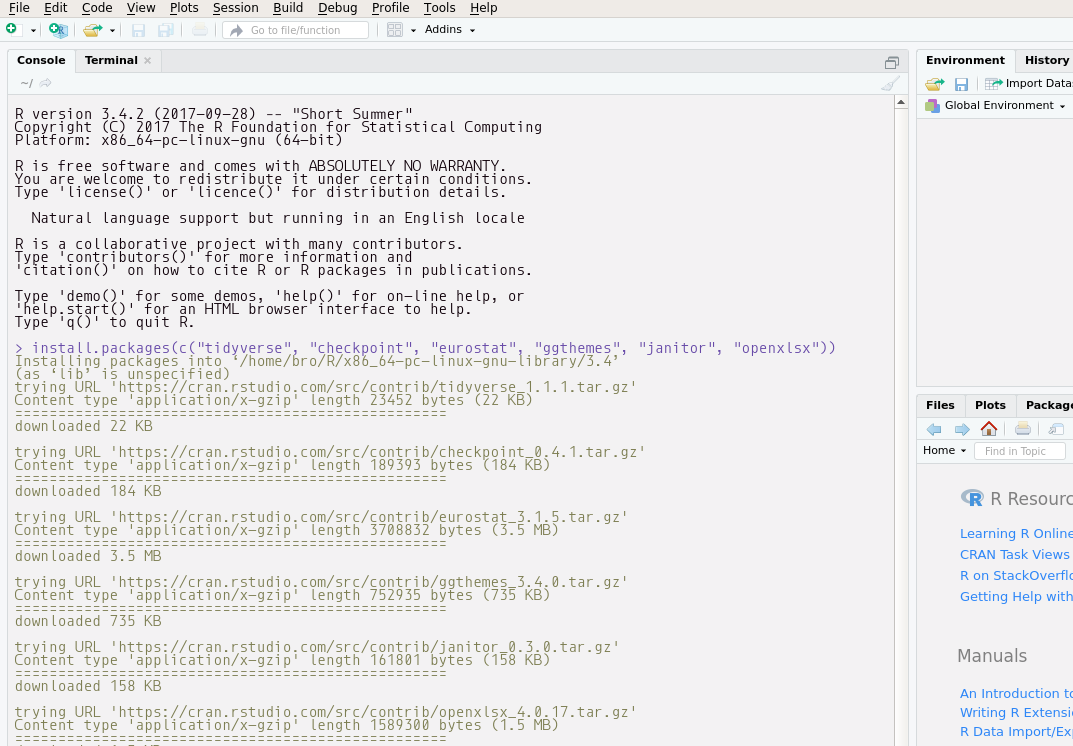
\includegraphics[width=14.9in]{pics/install_packages}

or go to the \textbf{Packages} pane and then click on \emph{Install}:

\includegraphics{pics/rstudio_install_packages.gif}

\hypertarget{the-author}{%
\subsection*{The author}\label{the-author}}
\addcontentsline{toc}{subsection}{The author}

My name is Bruno Rodrigues and I program almost exclusively in R and
have been teaching some R courses for a few years now (first started
teaching for students at the Université of Strasbourg). These notes are
an update of those I used at the time, plus a lot of things I've learned
about R In my free time I like cooking, working out and
\href{https://www.brodrigues.co}{blogging}, while listening to
\href{http://www.fipradio.fr/player}{Fip}. I also like to get my butt
handed to me by playing roguelikes such as
\href{http://nethack.wikia.com/wiki/NetHack}{NetHack}, for which I wrote
a \href{https://github.com/b-rodrigues/nethack}{package} that contains
functions to analyze the data that is saved on your computer after you
win or lose (it will be lose 99\% of the time) the game.

You can follow me on
\href{https://www.twitter.com/brodriguesco}{twitter}, I tweet mostly
about R or what's happening in Luxembourg.

\hypertarget{getting-to-know-rstudio}{%
\section{Getting to know RStudio}\label{getting-to-know-rstudio}}

\hypertarget{panes}{%
\subsection{Panes}\label{panes}}

RStudio is divided into different panes. Each pane has a specific
function. The gif below shows some of these panes:

\includegraphics{pics/rstudio_panes.gif}

Take some time to look around what each pane shows you. Some panes are
empty; for example the \emph{Plots} pane or the \emph{Viewer} pane.
\emph{Plots} shows you the plots you make. You can browse the plots and
save them. We will see this in more detail in a later chapter.
\emph{Viewer} shows you previews of documents that you generate with R.
More on this later.

\hypertarget{console}{%
\subsection{Console}\label{console}}

The \emph{Console} pane is where you can execute R code. Write the
following in the console:

\begin{Shaded}
\begin{Highlighting}[]
\DecValTok{2} \OperatorTok{+}\StringTok{ }\DecValTok{3}
\end{Highlighting}
\end{Shaded}

and you'll get the answer, \texttt{5}. However, do not write a lot of
lines in the console. It is better write your code inside a script.

\hypertarget{scripts}{%
\subsection{Scripts}\label{scripts}}

Look at the gif below:

\includegraphics{pics/rstudio_new_script.gif}

In this gif, we see the user creating a new R script. R scripts are
simple text files that hold R code. Think of \texttt{.do} files in STATA
or \texttt{.c} files for C. R scripts have the extension \texttt{.r} or
\texttt{.R}.

It is possible to create a lot of other files. We'll take a look at
\texttt{R\ Markdown} files later.

\hypertarget{the-help-pane}{%
\subsubsection{The help pane}\label{the-help-pane}}

The \emph{Help} pane allows you to consult documentation for functions
or packages. The gif below shows how it works:

\includegraphics{pics/rstudio_help.gif}

you can also access help using the following syntax: \texttt{?lm}. This
will bring up the documentation for the function \texttt{lm()}. You can
also type \texttt{??lm} which will look for the string \texttt{lm} in
every package.

\hypertarget{the-environment-pane}{%
\subsubsection{The Environment pane}\label{the-environment-pane}}

The \emph{Environment} pane shows every object created in the current
section. It is especially useful if you have defined lists or have
loaded data into R as it makes it easy to explore these more complex
objects.

\hypertarget{options}{%
\subsection{Options}\label{options}}

It is also possible to customize RStudio's look and feel:

\includegraphics{pics/rstudio_options.gif}

Take some time to go through the options.

\hypertarget{keyboard-shortcuts}{%
\subsection{Keyboard shortcuts}\label{keyboard-shortcuts}}

It is a good idea to familiarize yourself with at least some keyboard
shortcuts. This is more convenient than having to move the mouse around:

\includegraphics{pics/rstudio_shortcuts.gif}

If there is only one keyboard shortcut you need to know, it's
\texttt{Ctrl-Enter} that executes a line of code from your script.
However, these other shortcuts are also worth knowing:

\begin{itemize}
\tightlist
\item
  \texttt{CTRL-ALT-R}: run entire script
\item
  \texttt{CTRL-ALT-UP\ or\ DOWN}: make cursor taller or shorter,
  allowing you to edit multiple lines at the same time
\item
  \texttt{CTRL-F}: Search and replace
\item
  \texttt{ALT-UP\ or\ DOWN}: Move line up or down
\item
  \texttt{CTRL-SHIFT-C}: Comment/uncomment line
\item
  \texttt{ALT-SHIFT-K}: Bring up the list of keyboard shortcuts
\item
  \texttt{CTRL-SHIFT-M}: Insert the pipe operator
  (\texttt{\%\textgreater{}\%}, more on this later)
\item
  \texttt{CTRL-S}: Save script
\end{itemize}

This is just a few keyboard shortcuts that I personally find useful.
However, I strongly advise you to learn and use whatever shortcuts are
useful to you!

\hypertarget{projects}{%
\subsection{Projects}\label{projects}}

One of the best features of RStudio are projects. Creating a project is
simple; the gif below shows how you can create a project and how you can
switch between projects.

\includegraphics{pics/rstudio_projects.gif}

Projects make a lot of things easier, such as managing paths. More on
this in the chapter about reading data. Another useful feature of
projects is that the scripts you open in project A will stay open even
if you switch to another project B, and then switch back to the project
A again.

You can also use version control (with git) inside a project. Version
control is very useful, but I won't discuss it here. You can find a lot
of resources online to get you started with git.

\hypertarget{history}{%
\subsection{History}\label{history}}

The \emph{History} pane saves all the previous lines you executed. You
can then select these lines and send them back to the console or the
script.

\includegraphics{pics/rstudio_history.gif}

\hypertarget{plots}{%
\subsection{Plots}\label{plots}}

All the plots you make during a session are visible in the \emph{Plots}
pane. From there, you can export them in different formats.

\includegraphics{pics/rstudio_plots.gif}

The plots shown in the gif are made using basic R functions. Later, we
will learn how to make nicer looking plots using the package
\texttt{ggplot2}.

\hypertarget{addins}{%
\subsection{Addins}\label{addins}}

Some packages install addins, which are accessible through the addins
button:

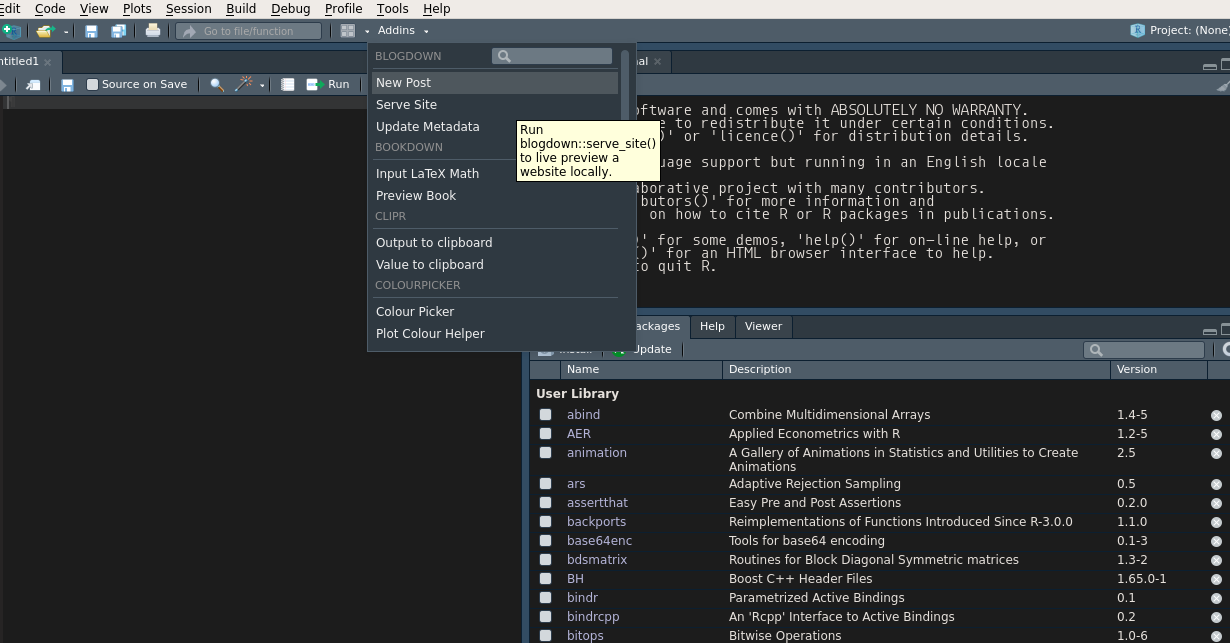
\includegraphics[width=17.08in]{pics/rstudio_addins}

This addins make it easier to use some functions and you can read more
about them
\href{https://rstudio.github.io/rstudioaddins/\#overview}{here}.

My favorite addins are the ones you get when installing the
\texttt{\{datapasta\}} package. Read more about it
\href{https://github.com/MilesMcBain/datapasta}{here}.

\hypertarget{exercises}{%
\subsection{Exercises}\label{exercises}}

\hypertarget{exercise-1}{%
\subsubsection*{Exercise 1}\label{exercise-1}}
\addcontentsline{toc}{subsubsection}{Exercise 1}

Change the look and feel of RStudio to suit your tastes! I personally
like to move the console to the right and use a dark theme. Take some 5
minutes to customize it and browse through all the options.

\hypertarget{packages}{%
\section{Packages}\label{packages}}

You can think of packages as addons that extend R's core functionality.
You can browse all available packages on
\href{https://cloud.r-project.org/}{CRAN}. To make it easier to find
what you might be interested in, you can also browse the
\href{https://cloud.r-project.org/web/views/}{CRAN Task Views}. Each
package has a landing page that summarises its dependencies, version
number etc. For example, for the \texttt{dplyr} package:
\url{https://cran.r-project.org/web/packages/dplyr/index.html}. Take a
look at the \emph{Downloads} section, and especially at the Reference
Manual and Vignettes:

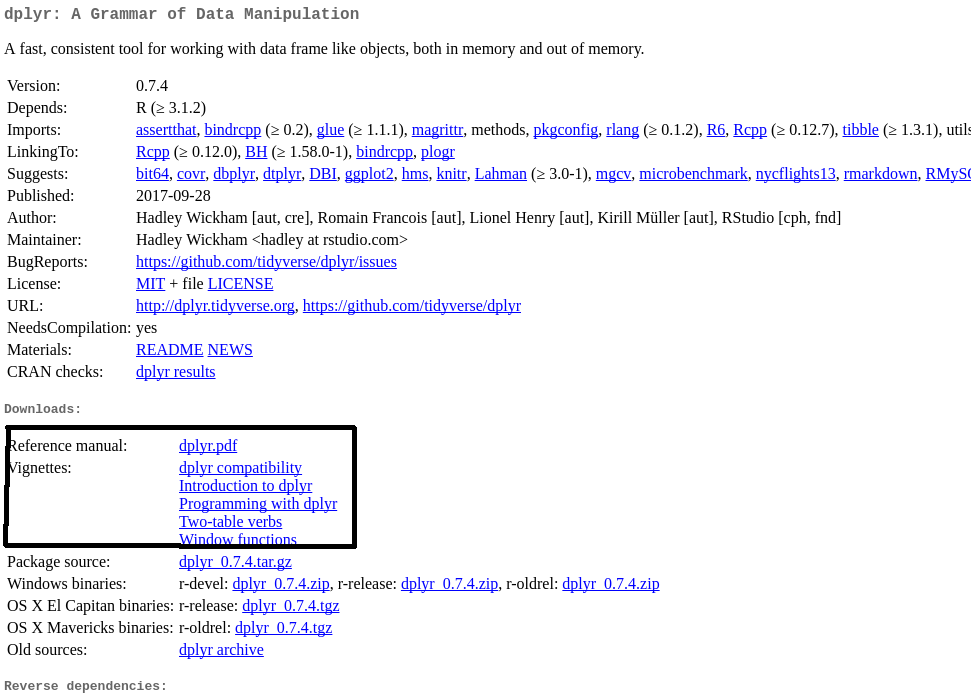
\includegraphics[width=13.49in]{pics/packages_vignette}

Vignettes are valuable documents; inside vignettes, the purpose of the
package is explained in plain English, usually with accompanying
examples. The reference manuals list the available functions inside the
packages. You can also find vignettes from within Rstudio:

\includegraphics{pics/rstudio_vignette.gif}

Go to the \emph{Packages} pane and click on the package you're
interested in. Then you can consult the help for the functions that come
with the package as well as the package's vignettes.

Once you installed a package, you have to load it before you can use it.
To load packages you use the \texttt{library()} function:

\begin{Shaded}
\begin{Highlighting}[]
\KeywordTok{library}\NormalTok{(dplyr)}
\KeywordTok{library}\NormalTok{(janitor)}
\CommentTok{# and so on...}
\end{Highlighting}
\end{Shaded}

If you only need to use one single function once, you don't need to load
an entire package. You can write the following:

\begin{Shaded}
\begin{Highlighting}[]
\NormalTok{dplyr}\OperatorTok{::}\KeywordTok{full_join}\NormalTok{(A, B)}
\end{Highlighting}
\end{Shaded}

using the \texttt{::} operator, you can access functions from packages
without having to load the whole package beforehand.

It is possible and easy to create your own packages. This is useful if
you have to write a lot of functions that you use daily. We will lean
about that, in Chapter 11.

\hypertarget{data-types-and-objects}{%
\section{Data types and objects}\label{data-types-and-objects}}

All objects in R have a given \emph{type}. You already know most of
them, as these types are also used in mathematics. Integers, floating
point numbers, or floats, matrices, etc, are all objects you are already
familiar with. But R has other, maybe lesser known data types (that you
can find in a lot of other programming languages) that you need to
become familiar with. But first, we need to learn how to assign a value
to a variable. This can be done in two ways:

\begin{Shaded}
\begin{Highlighting}[]
\NormalTok{a <-}\StringTok{ }\DecValTok{3}
\end{Highlighting}
\end{Shaded}

or

\begin{Shaded}
\begin{Highlighting}[]
\NormalTok{a <-}\StringTok{ }\DecValTok{3}
\end{Highlighting}
\end{Shaded}

there is almost no difference between these two approaches. You would
need to pay attention to this, and use \texttt{\textless{}-} in very
specific situations to which you will very likely never be confronted
to.

Another thing you must know before going further is that you can convert
from one type to another using functions that start with \texttt{as.()},
such as \texttt{as.character()}, \texttt{as.numeric()},
\texttt{as.logical()}, etc\ldots{} For example, \texttt{as.character(1)}
converts the number \texttt{1} to the character (or string) ``1''. There
are also \texttt{is.character()}, \texttt{is.numeric()} and so on that
test if the object is of the required class. These functions exist for
each object type, and are very useful. Make sure you remember them!

\hypertarget{the-numeric-class}{%
\subsection{\texorpdfstring{The \texttt{numeric}
class}{The numeric class}}\label{the-numeric-class}}

To define single numbers, you can do the following:

\begin{Shaded}
\begin{Highlighting}[]
\NormalTok{a <-}\StringTok{ }\DecValTok{3}
\end{Highlighting}
\end{Shaded}

The \texttt{class()} function allows you to check the class of an
object:

\begin{Shaded}
\begin{Highlighting}[]
\KeywordTok{class}\NormalTok{(a)}
\end{Highlighting}
\end{Shaded}

\begin{verbatim}
## [1] "numeric"
\end{verbatim}

Decimals are defined with the character \texttt{.}:

\begin{Shaded}
\begin{Highlighting}[]
\NormalTok{a <-}\StringTok{ }\FloatTok{3.14}
\end{Highlighting}
\end{Shaded}

\hypertarget{the-character-class}{%
\subsection{\texorpdfstring{The \texttt{character}
class}{The character class}}\label{the-character-class}}

Use \texttt{"\ "} to define characters (called strings in other
programming languages):

\begin{Shaded}
\begin{Highlighting}[]
\NormalTok{a <-}\StringTok{ "this is a string"}
\end{Highlighting}
\end{Shaded}

\begin{Shaded}
\begin{Highlighting}[]
\KeywordTok{class}\NormalTok{(a)}
\end{Highlighting}
\end{Shaded}

\begin{verbatim}
## [1] "character"
\end{verbatim}

A very nice package to work with characters is \texttt{\{stringr\}},
which is also part of the \texttt{\{tidyverse\}}.

\hypertarget{the-factor-class}{%
\subsection{\texorpdfstring{The \texttt{factor}
class}{The factor class}}\label{the-factor-class}}

Factors look like characters, but are very different. They are the
representation of categorical variables. A \texttt{\{tidyverse\}}
package to work with factors is \texttt{\{forcats\}}. You would rarely
use factor variables outside of datasets, so for now, it is enough to
know that this class exists. We are going to manipulate factor variables
in the next chatper 5.

\hypertarget{the-date-class}{%
\subsection{\texorpdfstring{The \texttt{Date}
class}{The Date class}}\label{the-date-class}}

Dates also look like characters, but are very different too:

\begin{Shaded}
\begin{Highlighting}[]
\KeywordTok{as.Date}\NormalTok{(}\StringTok{"2019/03/19"}\NormalTok{)}
\end{Highlighting}
\end{Shaded}

\begin{verbatim}
## [1] "2019-03-19"
\end{verbatim}

\begin{Shaded}
\begin{Highlighting}[]
\KeywordTok{class}\NormalTok{(}\KeywordTok{as.Date}\NormalTok{(}\StringTok{"2019/03/19"}\NormalTok{))}
\end{Highlighting}
\end{Shaded}

\begin{verbatim}
## [1] "Date"
\end{verbatim}

Manipulating dates and time can be tricky, but thankfully there's a
\texttt{\{tidyverse\}} package for that, called \texttt{\{lubridate\}}.
We are going to go over this package in Chapter 5.

\hypertarget{vectors-and-matrices}{%
\subsection{Vectors and matrices}\label{vectors-and-matrices}}

You can create a vector in different ways. But first of all, it is
important to understand that a vector in most programming languages is
nothing more than a list of things. These things can be numbers (either
integers or floats), strings, or even other vectors.

\hypertarget{the-c-function}{%
\subsubsection{\texorpdfstring{The \texttt{c()}
function}{The c() function}}\label{the-c-function}}

A very important function that allows you to build a vector is
\texttt{c()}:

\begin{Shaded}
\begin{Highlighting}[]
\NormalTok{a <-}\StringTok{ }\KeywordTok{c}\NormalTok{(}\DecValTok{1}\NormalTok{,}\DecValTok{2}\NormalTok{,}\DecValTok{3}\NormalTok{,}\DecValTok{4}\NormalTok{,}\DecValTok{5}\NormalTok{)}
\end{Highlighting}
\end{Shaded}

This creates a vector with elements 1, 2, 3, 4, 5. If you check its
class:

\begin{Shaded}
\begin{Highlighting}[]
\KeywordTok{class}\NormalTok{(a)}
\end{Highlighting}
\end{Shaded}

\begin{verbatim}
## [1] "numeric"
\end{verbatim}

This can be confusing: you where probably expecting a to be of class
\emph{vector} or something similar. This is not the case if you use
\texttt{c()} to create the vector, because \texttt{c()} doesn't build a
vector in the mathematical sense, but rather a list with numbers.
Checking its dimension:

\begin{Shaded}
\begin{Highlighting}[]
\KeywordTok{dim}\NormalTok{(a)}
\end{Highlighting}
\end{Shaded}

\begin{verbatim}
## NULL
\end{verbatim}

returns \texttt{NULL} because a list doesn't have a dimension, that's
why the \texttt{dim()} function returns \texttt{NULL}. If you want to
create a true vector, you need to use \texttt{cbind()} or
\texttt{rbind()}.

\hypertarget{cbind-and-rbind}{%
\subsubsection{\texorpdfstring{\texttt{cbind()} and
\texttt{rbind()}}{cbind() and rbind()}}\label{cbind-and-rbind}}

You can create a \emph{true} vector with \texttt{cbind()}:

\begin{Shaded}
\begin{Highlighting}[]
\NormalTok{a <-}\StringTok{ }\KeywordTok{cbind}\NormalTok{(}\DecValTok{1}\NormalTok{,}\DecValTok{2}\NormalTok{,}\DecValTok{3}\NormalTok{,}\DecValTok{4}\NormalTok{,}\DecValTok{5}\NormalTok{)}
\end{Highlighting}
\end{Shaded}

Check its class now:

\begin{Shaded}
\begin{Highlighting}[]
\KeywordTok{class}\NormalTok{(a)}
\end{Highlighting}
\end{Shaded}

\begin{verbatim}
## [1] "matrix"
\end{verbatim}

This is exactly what we expected. Let's check its dimension:

\begin{Shaded}
\begin{Highlighting}[]
\KeywordTok{dim}\NormalTok{(a)}
\end{Highlighting}
\end{Shaded}

\begin{verbatim}
## [1] 1 5
\end{verbatim}

This returns the dimension of \texttt{a} using the LICO notation (number
of LInes first, the number of COlumns).

It is also possible to bind vectors together to create a matrix.

\begin{Shaded}
\begin{Highlighting}[]
\NormalTok{b <-}\StringTok{ }\KeywordTok{cbind}\NormalTok{(}\DecValTok{6}\NormalTok{,}\DecValTok{7}\NormalTok{,}\DecValTok{8}\NormalTok{,}\DecValTok{9}\NormalTok{,}\DecValTok{10}\NormalTok{)}
\end{Highlighting}
\end{Shaded}

Now let's put vector \texttt{a} and \texttt{b} into a matrix called
\texttt{matrix\_c} using \texttt{rbind()}. \texttt{rbind()} functions
the same way as \texttt{cbind()} but glues the vectors together by rows
and not by columns.

\begin{Shaded}
\begin{Highlighting}[]
\NormalTok{matrix_c <-}\StringTok{ }\KeywordTok{rbind}\NormalTok{(a,b)}
\KeywordTok{print}\NormalTok{(matrix_c)}
\end{Highlighting}
\end{Shaded}

\begin{verbatim}
##      [,1] [,2] [,3] [,4] [,5]
## [1,]    1    2    3    4    5
## [2,]    6    7    8    9   10
\end{verbatim}

\hypertarget{the-matrix-class}{%
\subsubsection{\texorpdfstring{The \texttt{matrix}
class}{The matrix class}}\label{the-matrix-class}}

R also has support for matrices. For example, you can create a matrix of
dimension (5,5) filled with 0's with the \texttt{matrix()} function:

\begin{Shaded}
\begin{Highlighting}[]
\NormalTok{matrix_a <-}\StringTok{ }\KeywordTok{matrix}\NormalTok{(}\DecValTok{0}\NormalTok{, nrow <-}\StringTok{ }\DecValTok{5}\NormalTok{, ncol <-}\StringTok{ }\DecValTok{5}\NormalTok{)}
\end{Highlighting}
\end{Shaded}

If you want to create the following matrix:

\[
B <- \left(
\begin{array}{ccc}
 2 & 4 & 3 \\
 1 & 5 & 7
\end{array} \right)
\]

you would do it like this:

\begin{Shaded}
\begin{Highlighting}[]
\NormalTok{B <-}\StringTok{ }\KeywordTok{matrix}\NormalTok{(}\KeywordTok{c}\NormalTok{(}\DecValTok{2}\NormalTok{, }\DecValTok{4}\NormalTok{, }\DecValTok{3}\NormalTok{, }\DecValTok{1}\NormalTok{, }\DecValTok{5}\NormalTok{, }\DecValTok{7}\NormalTok{), nrow <-}\StringTok{ }\DecValTok{2}\NormalTok{, byrow <-}\StringTok{ }\OtherTok{TRUE}\NormalTok{)}
\end{Highlighting}
\end{Shaded}

The option \texttt{byrow\ \textless{}-\ TRUE} means that the rows of the
matrix will be filled first.

You can access individual elements of \texttt{matrix\_a} like so:

\begin{Shaded}
\begin{Highlighting}[]
\NormalTok{matrix_a[}\DecValTok{2}\NormalTok{, }\DecValTok{3}\NormalTok{]}
\end{Highlighting}
\end{Shaded}

\begin{verbatim}
## [1] 0
\end{verbatim}

and R returns its value, 0. We can assign a new value to this element if
we want. Try:

\begin{Shaded}
\begin{Highlighting}[]
\NormalTok{matrix_a[}\DecValTok{2}\NormalTok{, }\DecValTok{3}\NormalTok{] <-}\StringTok{ }\DecValTok{7}
\end{Highlighting}
\end{Shaded}

and now take a look at \texttt{matrix\_a} again.

\begin{Shaded}
\begin{Highlighting}[]
\KeywordTok{print}\NormalTok{(matrix_a)}
\end{Highlighting}
\end{Shaded}

\begin{verbatim}
##      [,1] [,2] [,3] [,4] [,5]
## [1,]    0    0    0    0    0
## [2,]    0    0    7    0    0
## [3,]    0    0    0    0    0
## [4,]    0    0    0    0    0
## [5,]    0    0    0    0    0
\end{verbatim}

Recall our vector \texttt{b}:

\begin{Shaded}
\begin{Highlighting}[]
\NormalTok{b <-}\StringTok{ }\KeywordTok{cbind}\NormalTok{(}\DecValTok{6}\NormalTok{,}\DecValTok{7}\NormalTok{,}\DecValTok{8}\NormalTok{,}\DecValTok{9}\NormalTok{,}\DecValTok{10}\NormalTok{)}
\end{Highlighting}
\end{Shaded}

To access its third element, you can simply write:

\begin{Shaded}
\begin{Highlighting}[]
\NormalTok{b[}\DecValTok{3}\NormalTok{]}
\end{Highlighting}
\end{Shaded}

\begin{verbatim}
## [1] 8
\end{verbatim}

\hypertarget{the-logical-class}{%
\subsection{\texorpdfstring{The \texttt{logical}
class}{The logical class}}\label{the-logical-class}}

This class is the result of logical comparisons, for example, if you
type:

\begin{Shaded}
\begin{Highlighting}[]
\DecValTok{4} \OperatorTok{>}\StringTok{ }\DecValTok{3}
\end{Highlighting}
\end{Shaded}

\begin{verbatim}
## [1] TRUE
\end{verbatim}

R returns true. If we save this in a variable \texttt{k}:

\begin{Shaded}
\begin{Highlighting}[]
\NormalTok{k <-}\StringTok{ }\DecValTok{4} \OperatorTok{>}\StringTok{ }\DecValTok{3}
\end{Highlighting}
\end{Shaded}

and check \texttt{k}'s class:

\begin{Shaded}
\begin{Highlighting}[]
\KeywordTok{class}\NormalTok{(k)}
\end{Highlighting}
\end{Shaded}

\begin{verbatim}
## [1] "logical"
\end{verbatim}

R returns \texttt{logical}. In other programming languages,
\texttt{logical}s are often called \texttt{bool}s.

A \texttt{logical} variable can only have two values, either
\texttt{TRUE} or \texttt{FALSE}.

\hypertarget{the-list-class}{%
\subsection{\texorpdfstring{The \texttt{list}
class}{The list class}}\label{the-list-class}}

The \texttt{list} class is a very flexible class, and thus, very useful.
You can put anything inside a list, such as numbers:

\begin{Shaded}
\begin{Highlighting}[]
\NormalTok{list1 <-}\StringTok{ }\KeywordTok{list}\NormalTok{(}\DecValTok{3}\NormalTok{, }\DecValTok{2}\NormalTok{)}
\end{Highlighting}
\end{Shaded}

or other lists constructed with \texttt{c()}:

\begin{Shaded}
\begin{Highlighting}[]
\NormalTok{list2 <-}\StringTok{ }\KeywordTok{list}\NormalTok{(}\KeywordTok{c}\NormalTok{(}\DecValTok{1}\NormalTok{, }\DecValTok{2}\NormalTok{), }\KeywordTok{c}\NormalTok{(}\DecValTok{3}\NormalTok{, }\DecValTok{4}\NormalTok{))}
\end{Highlighting}
\end{Shaded}

you can also put objects of different classes in the same list:

\begin{Shaded}
\begin{Highlighting}[]
\NormalTok{list3 <-}\StringTok{ }\KeywordTok{list}\NormalTok{(}\DecValTok{3}\NormalTok{, }\KeywordTok{c}\NormalTok{(}\DecValTok{1}\NormalTok{, }\DecValTok{2}\NormalTok{), }\StringTok{"lists are amazing!"}\NormalTok{)}
\end{Highlighting}
\end{Shaded}

and of course create list of lists:

\begin{Shaded}
\begin{Highlighting}[]
\NormalTok{my_lists <-}\StringTok{ }\KeywordTok{list}\NormalTok{(list1, list2, list3)}
\end{Highlighting}
\end{Shaded}

To check the contents of a list, you can use the structure function
\texttt{str()}:

\begin{Shaded}
\begin{Highlighting}[]
\KeywordTok{str}\NormalTok{(my_lists)}
\end{Highlighting}
\end{Shaded}

\begin{verbatim}
## List of 3
##  $ :List of 2
##   ..$ : num 3
##   ..$ : num 2
##  $ :List of 2
##   ..$ : num [1:2] 1 2
##   ..$ : num [1:2] 3 4
##  $ :List of 3
##   ..$ : num 3
##   ..$ : num [1:2] 1 2
##   ..$ : chr "lists are amazing!"
\end{verbatim}

or you can use RStudio's \emph{Environment} pane:

\includegraphics{pics/rstudio_environment_list.gif}

You can also create named lists:

\begin{Shaded}
\begin{Highlighting}[]
\NormalTok{list4 <-}\StringTok{ }\KeywordTok{list}\NormalTok{(}\StringTok{"a"}\NormalTok{ =}\StringTok{ }\DecValTok{2}\NormalTok{, }\StringTok{"b"}\NormalTok{ =}\StringTok{ }\DecValTok{8}\NormalTok{, }\StringTok{"c"}\NormalTok{ =}\StringTok{ "this is a named list"}\NormalTok{)}
\end{Highlighting}
\end{Shaded}

and you can access the elements in two ways:

\begin{Shaded}
\begin{Highlighting}[]
\NormalTok{list4[[}\DecValTok{1}\NormalTok{]]}
\end{Highlighting}
\end{Shaded}

\begin{verbatim}
## [1] 2
\end{verbatim}

or, for named lists:

\begin{Shaded}
\begin{Highlighting}[]
\NormalTok{list4}\OperatorTok{$}\NormalTok{c}
\end{Highlighting}
\end{Shaded}

\begin{verbatim}
## [1] "this is a named list"
\end{verbatim}

Lists are used extensively because they are so flexible. You can build
lists of datasets and apply functions to all the datasets at once, build
lists of models, lists of plots, etc\ldots{} In the later chapters we
are going to learn all about them. Actually, I use lists very often, but
never vectors or matrices. Lists are much more flexible and in R,
datasets behave like lists.

\hypertarget{the-data.frame-and-tibble-classes}{%
\subsection{\texorpdfstring{The \texttt{data.frame} and \texttt{tibble}
classes}{The data.frame and tibble classes}}\label{the-data.frame-and-tibble-classes}}

In the next chapter we are going to learn how to import datasets into R.
Once you import data, the resulting object is either a
\texttt{data.frame} or a \texttt{tibble} depending on which package you
used to import the data. \texttt{tibble}s extend \texttt{data.frame}s so
if you know about \texttt{data.frame} objects already, working with
\texttt{tibble}s will be very easy. \texttt{tibble}s have a better
\texttt{print()} method, and some other niceties. If you want to know
more, I go into more detail in my
\href{https://b-rodrigues.github.io/fput/tidyverse.html\#getting-data-into-r-with-readr-readxl-haven-and-what-are-tibbles}{other
book} but for our purposes, there's not much you need to know about
\texttt{data.frame} and \texttt{tibble} objects, apart that this is the
representation of a dataset when loaded into R.

However, I want to stress that these objects are central to R and are
thus very important. There are different ways to print a
\texttt{data.frame} or a \texttt{tibble} if you wish to inspect it. You
can use \texttt{View(my\_data)} to show the \texttt{my\_data}
\texttt{data.frame} in the \emph{View} pane of RStudio:

\includegraphics{pics/rstudio_view_data.gif}

You can also use the \texttt{str()} function:

\begin{Shaded}
\begin{Highlighting}[]
\KeywordTok{str}\NormalTok{(my_data)}
\end{Highlighting}
\end{Shaded}

And if you need to access an individual column, you can use the
\texttt{\$} sign, same as for a list:

\begin{Shaded}
\begin{Highlighting}[]
\NormalTok{my_data}\OperatorTok{$}\NormalTok{col1}
\end{Highlighting}
\end{Shaded}

\hypertarget{formulas}{%
\subsection{Formulas}\label{formulas}}

We will learn more about formulas later, but because it is an important
object, it is useful if you already know about them early on. A formula
is defined in the following way:

\begin{Shaded}
\begin{Highlighting}[]
\NormalTok{my_formula <-}\StringTok{ }\ErrorTok{~}\NormalTok{x}

\KeywordTok{class}\NormalTok{(my_formula)}
\end{Highlighting}
\end{Shaded}

\begin{verbatim}
## [1] "formula"
\end{verbatim}

Formula objects are defined using the \texttt{\textasciitilde{}} symbol.
Formulas are useful to define statistical models, for example for a
linear regression:

\begin{Shaded}
\begin{Highlighting}[]
\KeywordTok{lm}\NormalTok{(y }\OperatorTok{~}\StringTok{ }\NormalTok{x)}
\end{Highlighting}
\end{Shaded}

or also to define anonymous functions, but more on this later.

\hypertarget{models}{%
\subsection{Models}\label{models}}

A statistical model is an object like any other in R:

\begin{Shaded}
\begin{Highlighting}[]
\KeywordTok{data}\NormalTok{(mtcars)}

\NormalTok{my_model <-}\StringTok{ }\KeywordTok{lm}\NormalTok{(mpg }\OperatorTok{~}\StringTok{ }\NormalTok{hp, mtcars)}

\KeywordTok{class}\NormalTok{(my_model)}
\end{Highlighting}
\end{Shaded}

\begin{verbatim}
## [1] "lm"
\end{verbatim}

\texttt{my\_model} is an object of class \texttt{lm}. You can apply
different functions to a model object:

\begin{Shaded}
\begin{Highlighting}[]
\KeywordTok{summary}\NormalTok{(my_model)}
\end{Highlighting}
\end{Shaded}

\begin{verbatim}
## 
## Call:
## lm(formula = mpg ~ hp, data = mtcars)
## 
## Residuals:
##     Min      1Q  Median      3Q     Max 
## -5.7121 -2.1122 -0.8854  1.5819  8.2360 
## 
## Coefficients:
##             Estimate Std. Error t value Pr(>|t|)    
## (Intercept) 30.09886    1.63392  18.421  < 2e-16 ***
## hp          -0.06823    0.01012  -6.742 1.79e-07 ***
## ---
## Signif. codes:  0 '***' 0.001 '**' 0.01 '*' 0.05 '.' 0.1 ' ' 1
## 
## Residual standard error: 3.863 on 30 degrees of freedom
## Multiple R-squared:  0.6024, Adjusted R-squared:  0.5892 
## F-statistic: 45.46 on 1 and 30 DF,  p-value: 1.788e-07
\end{verbatim}

This class will be explored in later chapters.

\hypertarget{the-is.-and-as.-functions}{%
\subsection{\texorpdfstring{The \texttt{is.*()} and \texttt{as.*()}
functions}{The is.*() and as.*() functions}}\label{the-is.-and-as.-functions}}

\texttt{is.*()} and \texttt{as.*()} are very powerful, and this is the
right moment to introduce them. \texttt{is.*()} test the class of an
object:

\begin{Shaded}
\begin{Highlighting}[]
\KeywordTok{is.integer}\NormalTok{(}\DecValTok{5}\NormalTok{)}
\end{Highlighting}
\end{Shaded}

\begin{verbatim}
## [1] FALSE
\end{verbatim}

\begin{Shaded}
\begin{Highlighting}[]
\KeywordTok{is.character}\NormalTok{(}\DecValTok{198}\NormalTok{)}
\end{Highlighting}
\end{Shaded}

\begin{verbatim}
## [1] FALSE
\end{verbatim}

\texttt{as.*()} functions convert from one type to another:

\begin{Shaded}
\begin{Highlighting}[]
\KeywordTok{as.character}\NormalTok{(}\DecValTok{7}\NormalTok{)}
\end{Highlighting}
\end{Shaded}

\begin{verbatim}
## [1] "7"
\end{verbatim}

\begin{Shaded}
\begin{Highlighting}[]
\KeywordTok{as.numeric}\NormalTok{(}\StringTok{"23.12"}\NormalTok{)}
\end{Highlighting}
\end{Shaded}

\begin{verbatim}
## [1] 23.12
\end{verbatim}

but only if it makes sense:

\begin{Shaded}
\begin{Highlighting}[]
\KeywordTok{as.numeric}\NormalTok{(}\StringTok{"This will return NA"}\NormalTok{)}
\end{Highlighting}
\end{Shaded}

\begin{verbatim}
## Warning: NAs introduced by coercion
\end{verbatim}

\begin{verbatim}
## [1] NA
\end{verbatim}

Keep these in mind, because they are going to be very useful. The
\texttt{\{purrr\}} package introduces similar functions,
\texttt{is\_*()} and \texttt{as\_*()}. We will explore them in Chapter
9.

\hypertarget{exercises-1}{%
\subsection{Exercises}\label{exercises-1}}

\hypertarget{exercise-1-1}{%
\subsubsection*{Exercise 1}\label{exercise-1-1}}
\addcontentsline{toc}{subsubsection}{Exercise 1}

Try to create the following vector:

\[a = (6,3,8,9)\]

and add it this other vector:

\[b = (9,1,3,5)\]

and save the result to a new variable called \texttt{result}.

\hypertarget{exercise-2}{%
\subsubsection*{Exercise 2}\label{exercise-2}}
\addcontentsline{toc}{subsubsection}{Exercise 2}

Using \texttt{a} and \texttt{b} from before, try to get their dot
product.

Try with \texttt{a\ *\ b} in the R console. What happened? Try to find
the right function to get the dot product. Don't hesitate to google the
answer!

\hypertarget{exercise-3}{%
\subsubsection*{Exercise 3}\label{exercise-3}}
\addcontentsline{toc}{subsubsection}{Exercise 3}

How can you create a matrix of dimension (30,30) filled with 2's by only
using the function \texttt{matrix()}?

\hypertarget{exercise-4}{%
\subsubsection*{Exercise 4}\label{exercise-4}}
\addcontentsline{toc}{subsubsection}{Exercise 4}

Save your first name in a variable \texttt{a} and your surname in a
variable \texttt{b}. What does the function:

\begin{Shaded}
\begin{Highlighting}[]
\KeywordTok{paste}\NormalTok{(a, b)}
\end{Highlighting}
\end{Shaded}

do? Look at the help for \texttt{paste()} with \texttt{?paste} or using
the \emph{Help} pane in RStudio. What does the optional argument
\texttt{sep} do?

\hypertarget{exercise-5}{%
\subsubsection*{Exercise 5}\label{exercise-5}}
\addcontentsline{toc}{subsubsection}{Exercise 5}

Define the following variables: \texttt{a\ \textless{}-\ 8},
\texttt{b\ \textless{}-\ 3}, \texttt{c\ \textless{}-\ 19}. What do the
following lines check? What do they return?

\begin{Shaded}
\begin{Highlighting}[]
\NormalTok{a }\OperatorTok{>}\StringTok{ }\NormalTok{b}
\NormalTok{a }\OperatorTok{==}\StringTok{ }\NormalTok{b}
\NormalTok{a }\OperatorTok{!=}\StringTok{ }\NormalTok{b}
\NormalTok{a }\OperatorTok{<}\StringTok{ }\NormalTok{b}
\NormalTok{(a }\OperatorTok{>}\StringTok{ }\NormalTok{b) }\OperatorTok{&&}\StringTok{ }\NormalTok{(a }\OperatorTok{<}\StringTok{ }\NormalTok{c)}
\NormalTok{(a }\OperatorTok{>}\StringTok{ }\NormalTok{b) }\OperatorTok{&&}\StringTok{ }\NormalTok{(a }\OperatorTok{>}\StringTok{ }\NormalTok{c)}
\NormalTok{(a }\OperatorTok{>}\StringTok{ }\NormalTok{b) }\OperatorTok{||}\StringTok{ }\NormalTok{(a }\OperatorTok{<}\StringTok{ }\NormalTok{b)}
\end{Highlighting}
\end{Shaded}

\hypertarget{exercise-6}{%
\subsubsection*{Exercise 6}\label{exercise-6}}
\addcontentsline{toc}{subsubsection}{Exercise 6}

Define the following matrix:

\[
\text{matrix_a} = \left(
\begin{array}{ccc}
 9 & 4 & 12 \\
 5 & 0 & 7 \\
 2 & 6 & 8 \\
 9 & 2 & 9
\end{array} \right)
\]

\begin{itemize}
\tightlist
\item
  What does \texttt{matrix\_a\ \textgreater{}=\ 5} do?
\item
  What does \texttt{matrix\_a{[}\ ,\ 2{]}} do?
\item
  Can you find which function gives you the transpose of this matrix?
\end{itemize}

\hypertarget{exercise-7}{%
\subsubsection*{Exercise 7}\label{exercise-7}}
\addcontentsline{toc}{subsubsection}{Exercise 7}

Solve the following system of equations using the \texttt{solve()}
function:

\[
\left(
\begin{array}{cccc}
 9 & 4 & 12 & 2 \\
 5 & 0 & 7 & 9\\
 2 & 6 & 8 & 0\\
 9 & 2 & 9 & 11
\end{array} \right) \times \left(
\begin{array}{ccc}
 x \\
 y \\
 z \\
 t \\
\end{array}\right) =
\left(
\begin{array}{ccc}
7\\
18\\
1\\
0
\end{array}
\right)
\]

\hypertarget{exercise-8}{%
\subsubsection*{Exercise 8}\label{exercise-8}}
\addcontentsline{toc}{subsubsection}{Exercise 8}

Load the \texttt{mtcars} data (\texttt{mtcars} is include in R, so you
only need to use the \texttt{data()} function to load the data):

\begin{Shaded}
\begin{Highlighting}[]
\KeywordTok{data}\NormalTok{(mtcars)}
\end{Highlighting}
\end{Shaded}

if you run \texttt{class(mtcars)}, you get ``data.frame''. Try now with
\texttt{typeof(mtcars)}. The answer is now ``list''! This is because the
class of an object is an attribute of that object, which can even be
assigned by the user:

\begin{Shaded}
\begin{Highlighting}[]
\KeywordTok{class}\NormalTok{(mtcars) <-}\StringTok{ "don't do this"}

\KeywordTok{class}\NormalTok{(mtcars)}
\end{Highlighting}
\end{Shaded}

\begin{verbatim}
## [1] "don't do this"
\end{verbatim}

The type of an object is R's internal type of that object, which cannot
be manipulated by the user. It is always useful to know the type of an
object (not just its class). For example, in the particular case of data
frames, because the type of a data frame is a list, you can use all that
you learned about lists to manipulate data frames! Recall that
\texttt{\$} allowed you to select the element of a list for instance:

\begin{Shaded}
\begin{Highlighting}[]
\NormalTok{my_list <-}\StringTok{ }\KeywordTok{list}\NormalTok{(}\StringTok{"one"}\NormalTok{ =}\StringTok{ }\DecValTok{1}\NormalTok{, }\StringTok{"two"}\NormalTok{ =}\StringTok{ }\DecValTok{2}\NormalTok{, }\StringTok{"three"}\NormalTok{ =}\StringTok{ }\DecValTok{3}\NormalTok{)}

\NormalTok{my_list}\OperatorTok{$}\NormalTok{one}
\end{Highlighting}
\end{Shaded}

\begin{verbatim}
## [1] 1
\end{verbatim}

Because data frames are nothing but fancy lists, this is why you can
access columns the same way:

\begin{Shaded}
\begin{Highlighting}[]
\NormalTok{mtcars}\OperatorTok{$}\NormalTok{mpg}
\end{Highlighting}
\end{Shaded}

\begin{verbatim}
##  [1] 21.0 21.0 22.8 21.4 18.7 18.1 14.3 24.4 22.8 19.2 17.8 16.4 17.3 15.2
## [15] 10.4 10.4 14.7 32.4 30.4 33.9 21.5 15.5 15.2 13.3 19.2 27.3 26.0 30.4
## [29] 15.8 19.7 15.0 21.4
\end{verbatim}

\hypertarget{reading-and-writing-data}{%
\section{Reading and writing data}\label{reading-and-writing-data}}

In this chapter, we are going to import example datasets that are
available in R, \texttt{mtcars} and \texttt{iris}. I have converted
these datasets into several formats. Download those datasets
\href{https://github.com/b-rodrigues/modern_R/tree/master/datasets}{here}
if you want to follow the examples below. R can import some formats
without the need of external packages, such as the \texttt{.csv} format.
However, for other formats, you will need to use different packages.
Because there are a lot of different formats available I suggest you use
the \texttt{\{rio\}} package. \texttt{\{rio\}} is a wrapper around
different packages that import/export data in different formats. This
package is nice because you don't need to remember which package to use
to import, say, STATA datasets and then you need to remember which one
for SAS datasets, and so on. Read \texttt{\{rio\}}'s
\href{https://cran.r-project.org/web/packages/rio/vignettes/rio.html}{vignette}
for more details. Below I show some of \texttt{\{rio\}}'s functions
presented in the vignette. It is also possible to import data from
other, less ``traditional'' sources, such as your clipboard. Also note
that it is possible to import more than one dataset at once. There are
two ways of doing that, either by importing all the datasets, binding
their rows together and add a new variable with the name of the data, or
import all the datasets into a list, where each element of that list is
a data frame. We are going to explore this second option later.

\hypertarget{the-swiss-army-knife-of-data-import-and-export-rio}{%
\subsection{\texorpdfstring{The swiss army knife of data import and
export:
\texttt{\{rio\}}}{The swiss army knife of data import and export: \{rio\}}}\label{the-swiss-army-knife-of-data-import-and-export-rio}}

To import data with \texttt{\{rio\}}, \texttt{import()} is all you need:

\begin{Shaded}
\begin{Highlighting}[]
\KeywordTok{library}\NormalTok{(rio)}

\NormalTok{mtcars <-}\StringTok{ }\KeywordTok{import}\NormalTok{(}\StringTok{"datasets/mtcars.csv"}\NormalTok{)}
\end{Highlighting}
\end{Shaded}

\begin{Shaded}
\begin{Highlighting}[]
\KeywordTok{head}\NormalTok{(mtcars)}
\end{Highlighting}
\end{Shaded}

\begin{verbatim}
##    mpg cyl disp  hp drat    wt  qsec vs am gear carb
## 1 21.0   6  160 110 3.90 2.620 16.46  0  1    4    4
## 2 21.0   6  160 110 3.90 2.875 17.02  0  1    4    4
## 3 22.8   4  108  93 3.85 2.320 18.61  1  1    4    1
## 4 21.4   6  258 110 3.08 3.215 19.44  1  0    3    1
## 5 18.7   8  360 175 3.15 3.440 17.02  0  0    3    2
## 6 18.1   6  225 105 2.76 3.460 20.22  1  0    3    1
\end{verbatim}

\texttt{import()} needs the path to the data, and you can specify
additional options if needed. On a Windows computer, you have to pay
attention to the path; you cannot simply copy and paste it, because
paths in Windows use the \texttt{\textbackslash{}} symbol whereas R uses
\texttt{/} (just like on Linux or macOS). Importing a STATA or a SAS
file is done just the same:

\begin{Shaded}
\begin{Highlighting}[]
\NormalTok{mtcars_stata <-}\StringTok{ }\KeywordTok{import}\NormalTok{(}\StringTok{"datasets/mtcars.dta"}\NormalTok{)}
\KeywordTok{head}\NormalTok{(mtcars_stata)}
\end{Highlighting}
\end{Shaded}

\begin{verbatim}
##    mpg cyl disp  hp drat    wt  qsec vs am gear carb
## 1 21.0   6  160 110 3.90 2.620 16.46  0  1    4    4
## 2 21.0   6  160 110 3.90 2.875 17.02  0  1    4    4
## 3 22.8   4  108  93 3.85 2.320 18.61  1  1    4    1
## 4 21.4   6  258 110 3.08 3.215 19.44  1  0    3    1
## 5 18.7   8  360 175 3.15 3.440 17.02  0  0    3    2
## 6 18.1   6  225 105 2.76 3.460 20.22  1  0    3    1
\end{verbatim}

\begin{Shaded}
\begin{Highlighting}[]
\NormalTok{mtcars_sas <-}\StringTok{ }\KeywordTok{import}\NormalTok{(}\StringTok{"datasets/mtcars.sas7bdat"}\NormalTok{)}
\KeywordTok{head}\NormalTok{(mtcars_sas)}
\end{Highlighting}
\end{Shaded}

\begin{verbatim}
##    mpg cyl disp  hp drat    wt  qsec vs am gear carb
## 1 21.0   6  160 110 3.90 2.620 16.46  0  1    4    4
## 2 21.0   6  160 110 3.90 2.875 17.02  0  1    4    4
## 3 22.8   4  108  93 3.85 2.320 18.61  1  1    4    1
## 4 21.4   6  258 110 3.08 3.215 19.44  1  0    3    1
## 5 18.7   8  360 175 3.15 3.440 17.02  0  0    3    2
## 6 18.1   6  225 105 2.76 3.460 20.22  1  0    3    1
\end{verbatim}

It is also possible to import Excel files where each sheet is a single
table, but you will need \texttt{import\_list()} for that. The file
\texttt{multi.xlsx} has two sheets, each with a table in it:

\begin{Shaded}
\begin{Highlighting}[]
\NormalTok{multi <-}\StringTok{ }\KeywordTok{import_list}\NormalTok{(}\StringTok{"datasets/multi.xlsx"}\NormalTok{)}
\KeywordTok{str}\NormalTok{(multi)}
\end{Highlighting}
\end{Shaded}

\begin{verbatim}
## List of 2
##  $ mtcars:'data.frame':  32 obs. of  11 variables:
##   ..$ mpg : num [1:32] 21 21 22.8 21.4 18.7 18.1 14.3 24.4 22.8 19.2 ...
##   ..$ cyl : num [1:32] 6 6 4 6 8 6 8 4 4 6 ...
##   ..$ disp: num [1:32] 160 160 108 258 360 ...
##   ..$ hp  : num [1:32] 110 110 93 110 175 105 245 62 95 123 ...
##   ..$ drat: num [1:32] 3.9 3.9 3.85 3.08 3.15 2.76 3.21 3.69 3.92 3.92 ...
##   ..$ wt  : num [1:32] 2.62 2.88 2.32 3.21 3.44 ...
##   ..$ qsec: num [1:32] 16.5 17 18.6 19.4 17 ...
##   ..$ vs  : num [1:32] 0 0 1 1 0 1 0 1 1 1 ...
##   ..$ am  : num [1:32] 1 1 1 0 0 0 0 0 0 0 ...
##   ..$ gear: num [1:32] 4 4 4 3 3 3 3 4 4 4 ...
##   ..$ carb: num [1:32] 4 4 1 1 2 1 4 2 2 4 ...
##  $ iris  :'data.frame':  150 obs. of  5 variables:
##   ..$ Sepal.Length: num [1:150] 5.1 4.9 4.7 4.6 5 5.4 4.6 5 4.4 4.9 ...
##   ..$ Sepal.Width : num [1:150] 3.5 3 3.2 3.1 3.6 3.9 3.4 3.4 2.9 3.1 ...
##   ..$ Petal.Length: num [1:150] 1.4 1.4 1.3 1.5 1.4 1.7 1.4 1.5 1.4 1.5 ...
##   ..$ Petal.Width : num [1:150] 0.2 0.2 0.2 0.2 0.2 0.4 0.3 0.2 0.2 0.1 ...
##   ..$ Species     : chr [1:150] "setosa" "setosa" "setosa" "setosa" ...
\end{verbatim}

As you can see \texttt{multi} is a list of datasets. Told you lists were
very flexible! It is also possible to import all the datasets in a
single directory at once. For this, you first need a vector of paths:

\begin{Shaded}
\begin{Highlighting}[]
\NormalTok{paths <-}\StringTok{ }\KeywordTok{Sys.glob}\NormalTok{(}\StringTok{"datasets/unemployment/*.csv"}\NormalTok{)}
\end{Highlighting}
\end{Shaded}

\texttt{Sys.glob()} allows you to find files using a regular expression.
"datasets/unemployment/*.csv" matches all the \texttt{.csv} files inside
the ``datasets/unemployment/'' folder.

\begin{Shaded}
\begin{Highlighting}[]
\NormalTok{all_data <-}\StringTok{ }\KeywordTok{import_list}\NormalTok{(paths)}

\KeywordTok{str}\NormalTok{(all_data)}
\end{Highlighting}
\end{Shaded}

\begin{verbatim}
## List of 4
##  $ unemp_2013:'data.frame':  118 obs. of  8 variables:
##   ..$ Commune                   : chr [1:118] "Grand-Duche de Luxembourg" "Canton Capellen" "Dippach" "Garnich" ...
##   ..$ Total employed population : int [1:118] 223407 17802 1703 844 1431 4094 2146 971 1218 3002 ...
##   ..$ of which: Wage-earners    : int [1:118] 203535 15993 1535 750 1315 3800 1874 858 1029 2664 ...
##   ..$ of which: Non-wage-earners: int [1:118] 19872 1809 168 94 116 294 272 113 189 338 ...
##   ..$ Unemployed                : int [1:118] 19287 1071 114 25 74 261 98 45 66 207 ...
##   ..$ Active population         : int [1:118] 242694 18873 1817 869 1505 4355 2244 1016 1284 3209 ...
##   ..$ Unemployment rate (in %)  : num [1:118] 7.95 5.67 6.27 2.88 4.92 ...
##   ..$ Year                      : int [1:118] 2013 2013 2013 2013 2013 2013 2013 2013 2013 2013 ...
##  $ unemp_2014:'data.frame':  118 obs. of  8 variables:
##   ..$ Commune                   : chr [1:118] "Grand-Duche de Luxembourg" "Canton Capellen" "Dippach" "Garnich" ...
##   ..$ Total employed population : int [1:118] 228423 18166 1767 845 1505 4129 2172 1007 1268 3124 ...
##   ..$ of which: Wage-earners    : int [1:118] 208238 16366 1606 757 1390 3840 1897 887 1082 2782 ...
##   ..$ of which: Non-wage-earners: int [1:118] 20185 1800 161 88 115 289 275 120 186 342 ...
##   ..$ Unemployed                : int [1:118] 19362 1066 122 19 66 287 91 38 61 202 ...
##   ..$ Active population         : int [1:118] 247785 19232 1889 864 1571 4416 2263 1045 1329 3326 ...
##   ..$ Unemployment rate (in %)  : num [1:118] 7.81 5.54 6.46 2.2 4.2 ...
##   ..$ Year                      : int [1:118] 2014 2014 2014 2014 2014 2014 2014 2014 2014 2014 ...
##  $ unemp_2015:'data.frame':  118 obs. of  8 variables:
##   ..$ Commune                   : chr [1:118] "Grand-Duche de Luxembourg" "Canton Capellen" "Dippach" "Garnich" ...
##   ..$ Total employed population : int [1:118] 233130 18310 1780 870 1470 4130 2170 1050 1300 3140 ...
##   ..$ of which: Wage-earners    : int [1:118] 212530 16430 1620 780 1350 3820 1910 920 1100 2770 ...
##   ..$ of which: Non-wage-earners: int [1:118] 20600 1880 160 90 120 310 260 130 200 370 ...
##   ..$ Unemployed                : int [1:118] 18806 988 106 29 73 260 80 41 72 169 ...
##   ..$ Active population         : int [1:118] 251936 19298 1886 899 1543 4390 2250 1091 1372 3309 ...
##   ..$ Unemployment rate (in %)  : num [1:118] 7.46 5.12 5.62 3.23 4.73 ...
##   ..$ Year                      : int [1:118] 2015 2015 2015 2015 2015 2015 2015 2015 2015 2015 ...
##  $ unemp_2016:'data.frame':  118 obs. of  8 variables:
##   ..$ Commune                   : chr [1:118] "Grand-Duche de Luxembourg" "Canton Capellen" "Dippach" "Garnich" ...
##   ..$ Total employed population : int [1:118] 236100 18380 1790 870 1470 4160 2160 1030 1330 3150 ...
##   ..$ of which: Wage-earners    : int [1:118] 215430 16500 1640 780 1350 3840 1900 900 1130 2780 ...
##   ..$ of which: Non-wage-earners: int [1:118] 20670 1880 150 90 120 320 260 130 200 370 ...
##   ..$ Unemployed                : int [1:118] 18185 975 91 27 66 246 76 35 70 206 ...
##   ..$ Active population         : int [1:118] 254285 19355 1881 897 1536 4406 2236 1065 1400 3356 ...
##   ..$ Unemployment rate (in %)  : num [1:118] 7.15 5.04 4.84 3.01 4.3 ...
##   ..$ Year                      : int [1:118] 2016 2016 2016 2016 2016 2016 2016 2016 2016 2016 ...
\end{verbatim}

in a subsequent chapter we will learn how to actually use these lists of
datasets.

If you know that each dataset in each file has the same colmuns, you can
also import them directly into a single dataset by binding each dataset
together using \texttt{rbind\ =\ TRUE}:

\begin{Shaded}
\begin{Highlighting}[]
\NormalTok{bind_data <-}\StringTok{ }\KeywordTok{import_list}\NormalTok{(paths, }\DataTypeTok{rbind =} \OtherTok{TRUE}\NormalTok{)}
\KeywordTok{str}\NormalTok{(bind_data)}
\end{Highlighting}
\end{Shaded}

\begin{verbatim}
## 'data.frame':    472 obs. of  9 variables:
##  $ Commune                   : chr  "Grand-Duche de Luxembourg" "Canton Capellen" "Dippach" "Garnich" ...
##  $ Total employed population : int  223407 17802 1703 844 1431 4094 2146 971 1218 3002 ...
##  $ of which: Wage-earners    : int  203535 15993 1535 750 1315 3800 1874 858 1029 2664 ...
##  $ of which: Non-wage-earners: int  19872 1809 168 94 116 294 272 113 189 338 ...
##  $ Unemployed                : int  19287 1071 114 25 74 261 98 45 66 207 ...
##  $ Active population         : int  242694 18873 1817 869 1505 4355 2244 1016 1284 3209 ...
##  $ Unemployment rate (in %)  : num  7.95 5.67 6.27 2.88 4.92 ...
##  $ Year                      : int  2013 2013 2013 2013 2013 2013 2013 2013 2013 2013 ...
##  $ _file                     : chr  "datasets/unemployment/unemp_2013.csv" "datasets/unemployment/unemp_2013.csv" "datasets/unemployment/unemp_2013.csv" "datasets/unemployment/unemp_2013.csv" ...
##  - attr(*, ".internal.selfref")=<externalptr>
\end{verbatim}

This also add a further column called \texttt{\_file} indicating the
name of the file that contained the original data.

If something goes wrong, you might need to take a look at the underlying
function \texttt{\{rio\}} is actually using to import the file. Let's
look at the following example:

\begin{Shaded}
\begin{Highlighting}[]
\NormalTok{testdata <-}\StringTok{ }\KeywordTok{import}\NormalTok{(}\StringTok{"datasets/problems/mtcars.csv"}\NormalTok{)}

\KeywordTok{head}\NormalTok{(testdata)}
\end{Highlighting}
\end{Shaded}

\begin{verbatim}
##   mpg&cyl&disp&hp&drat&wt&qsec&vs&am&gear&carb
## 1          21&6&160&110&3.9&2.62&16.46&0&1&4&4
## 2         21&6&160&110&3.9&2.875&17.02&0&1&4&4
## 3        22.8&4&108&93&3.85&2.32&18.61&1&1&4&1
## 4      21.4&6&258&110&3.08&3.215&19.44&1&0&3&1
## 5       18.7&8&360&175&3.15&3.44&17.02&0&0&3&2
## 6       18.1&6&225&105&2.76&3.46&20.22&1&0&3&1
\end{verbatim}

as you can see, the import didn't work quite well! This is because the
separator is the \texttt{\&} for some reason. Because we are trying to
read a \texttt{.csv} file, \texttt{rio::import()} is using
\texttt{data.table::fread()} under the hood (you can read this in
\texttt{import()}'s help). If you then read
\texttt{data.table::fread()}'s help, you see that the \texttt{fread()}
function has an optional \texttt{sep\ =} argument that you can use to
specify the separator. You can use this argument in \texttt{import()}
too, and it will be passed down to \texttt{data.table::fread()}:

\begin{Shaded}
\begin{Highlighting}[]
\NormalTok{testdata <-}\StringTok{ }\KeywordTok{import}\NormalTok{(}\StringTok{"datasets/problems/mtcars.csv"}\NormalTok{, }\DataTypeTok{sep =} \StringTok{"&"}\NormalTok{)}

\KeywordTok{head}\NormalTok{(testdata)}
\end{Highlighting}
\end{Shaded}

\begin{verbatim}
##    mpg cyl disp  hp drat    wt  qsec vs am gear carb
## 1   21   6  160 110  3.9  2.62 16.46  0  1    4    4
## 2   21   6  160 110  3.9 2.875 17.02  0  1    4    4
## 3 22.8   4  108  93 3.85  2.32 18.61  1  1    4    1
## 4 21.4   6  258 110 3.08 3.215 19.44  1  0    3    1
## 5 18.7   8  360 175 3.15  3.44 17.02  0  0    3    2
## 6 18.1   6  225 105 2.76  3.46 20.22  1  0    3    1
\end{verbatim}

\texttt{export()} allows you to write data to disk, by simply providing
the path and name of the file you wish to save.

\begin{Shaded}
\begin{Highlighting}[]
\KeywordTok{export}\NormalTok{(testdata, }\StringTok{"path/where/to/save/testdata.csv"}\NormalTok{)}
\end{Highlighting}
\end{Shaded}

If you end the name with \texttt{.csv} the file is exported to the csv
format, if instead you write \texttt{.dta} the data will be exported to
the STATA format, and so on.

If you wish to export to Excel, this is possible, but it may require
that you change a file on your computer (you only have to do this once).
Try running:

\begin{Shaded}
\begin{Highlighting}[]
\KeywordTok{export}\NormalTok{(testdata, }\StringTok{"path/where/to/save/testdata.xlsx"}\NormalTok{)}
\end{Highlighting}
\end{Shaded}

if this results in an error, try the following:

\begin{itemize}
\tightlist
\item
  Run the following lines in Rstudio:
\end{itemize}

\begin{Shaded}
\begin{Highlighting}[]
\ControlFlowTok{if}\NormalTok{(}\OperatorTok{!}\KeywordTok{file.exists}\NormalTok{(}\StringTok{"~/.Rprofile"}\NormalTok{)) }\CommentTok{# only create if not already there}
    \KeywordTok{file.create}\NormalTok{(}\StringTok{"~/.Rprofile"}\NormalTok{)    }\CommentTok{# (don't overwrite it)}
\KeywordTok{file.edit}\NormalTok{(}\StringTok{"~/.Rprofile"}\NormalTok{)}
\end{Highlighting}
\end{Shaded}

These lines, taken shamelessly from
\href{https://csgillespie.github.io/efficientR/3-3-r-startup.html\#rprofile}{Efficient
R programming} (go read it, it's a very great resource) look for and
open the \texttt{.Rprofile} file which is a file that is run every time
you open Rstudio. This means that you can put any line of code there
that will always be executed whenever you launch Rstudio.

\begin{itemize}
\tightlist
\item
  Add this line to the file:
\end{itemize}

\begin{Shaded}
\begin{Highlighting}[]
\KeywordTok{Sys.setenv}\NormalTok{(}\StringTok{"R_ZIPCMD"}\NormalTok{ =}\StringTok{ "C:/Program Files (x86)/Rtools/zip.exe"}\NormalTok{)}
\end{Highlighting}
\end{Shaded}

This tells Rstudio to use \texttt{zip.exe} as the default zip tool,
which is needed to export files to the Excel format. Try it out by
restarting Rstudio, and then running the following lines:

\begin{Shaded}
\begin{Highlighting}[]
\KeywordTok{library}\NormalTok{(rio)}

\KeywordTok{data}\NormalTok{(mtcars)}

\KeywordTok{export}\NormalTok{(mtcars, }\StringTok{"mtcars.xlsx"}\NormalTok{)}
\end{Highlighting}
\end{Shaded}

You should find the \texttt{mtcars.xlsx} inside your working directory.
You can check what is your working directory with \texttt{getwd()}.

\texttt{\{rio\}} should cover all your needs, but if not, there is very
likely a package out there that will import the data you need.

\hypertarget{writing-any-object-to-disk}{%
\subsection{Writing any object to
disk}\label{writing-any-object-to-disk}}

\texttt{\{rio\}} is an amazing package, but is only able to write
tabular representations of data. What if you would like to save, say, a
list containing any arbitrary object? This is possible with the
\texttt{saveRDS()} function. Literally anything can be saved with
\texttt{saveRDS()}:

\begin{Shaded}
\begin{Highlighting}[]
\NormalTok{my_list <-}\StringTok{ }\KeywordTok{list}\NormalTok{(}\StringTok{"this is a list"}\NormalTok{, }\KeywordTok{list}\NormalTok{(}\StringTok{"which contains a list"}\NormalTok{, }\DecValTok{12}\NormalTok{), }\KeywordTok{c}\NormalTok{(}\DecValTok{1}\NormalTok{, }\DecValTok{2}\NormalTok{, }\DecValTok{3}\NormalTok{, }\DecValTok{4}\NormalTok{), }\KeywordTok{matrix}\NormalTok{(}\KeywordTok{c}\NormalTok{(}\DecValTok{2}\NormalTok{, }\DecValTok{4}\NormalTok{,}
\DecValTok{3}\NormalTok{, }\DecValTok{1}\NormalTok{, }\DecValTok{5}\NormalTok{, }\DecValTok{7}\NormalTok{), }\DataTypeTok{nrow =} \DecValTok{2}\NormalTok{))}

\KeywordTok{str}\NormalTok{(my_list)}
\end{Highlighting}
\end{Shaded}

\begin{verbatim}
## List of 4
##  $ : chr "this is a list"
##  $ :List of 2
##   ..$ : chr "which contains a list"
##   ..$ : num 12
##  $ : num [1:4] 1 2 3 4
##  $ : num [1:2, 1:3] 2 4 3 1 5 7
\end{verbatim}

\texttt{my\_list} is a list containing a string, a list which contains a
string and a number, a vector and a matrix\ldots{} Now suppose that
computing this list takes a very long time. For example, imagine that
each element of the list is the result of estimating a very complex
model on a simulated dataset, which takes hours to simulate. Because
this takes so long to compute, you'd want to save it to disk. This is
possible with \texttt{saveRDS()}:

\begin{Shaded}
\begin{Highlighting}[]
\KeywordTok{saveRDS}\NormalTok{(my_list, }\StringTok{"my_list.RDS"}\NormalTok{)}
\end{Highlighting}
\end{Shaded}

The next day, after having freshly started your computer and launched
RStudio, it is possible to retrieve the object exactly like it was using
\texttt{readRDS()}:

\begin{Shaded}
\begin{Highlighting}[]
\NormalTok{my_list <-}\StringTok{ }\KeywordTok{readRDS}\NormalTok{(}\StringTok{"my_list.RDS"}\NormalTok{)}

\KeywordTok{str}\NormalTok{(my_list)}
\end{Highlighting}
\end{Shaded}

\begin{verbatim}
## List of 4
##  $ : chr "this is a list"
##  $ :List of 2
##   ..$ : chr "which contains a list"
##   ..$ : num 12
##  $ : num [1:4] 1 2 3 4
##  $ : num [1:2, 1:3] 2 4 3 1 5 7
\end{verbatim}

Even if you want to save a regular dataset, using \texttt{saveRDS()}
might be a good idea because the data gets compressed if you add the
option \texttt{compress\ =\ TRUE} to \texttt{saveRDS()}. However keep in
mind that this will only be readable by R, so if you need to share this
data with colleagues that use another tool, save it in another format.

\hypertarget{using-rstudio-projects-to-manage-paths}{%
\subsection{Using RStudio projects to manage
paths}\label{using-rstudio-projects-to-manage-paths}}

Managing paths can be painful, especially if you're collaborating with a
colleague and both of you saved the data in paths that are different.
Whenever one of you wants to work on the script, the path will need to
be adapted first. The best way to avoid that is to use projects with
RStudio.

\includegraphics{pics/rstudio_projects.gif}

Imagine that you are working on a project entitled ``housing''. You will
create a folder called ``housing'' somewhere on your computer and inside
this folder have another folder called ``data'', then a bunch of other
folders containing different files or the outputs of your analysis. What
matters here is that you have a folder called ``data'' which contains
the datasets you will ananlyze. When you are inside an RStudio project,
granted that you chose your ``housing'' folder as the folder to host the
project, you can read the data by simply specifying the path like so:

\begin{Shaded}
\begin{Highlighting}[]
\NormalTok{my_data <-}\StringTok{ }\KeywordTok{import}\NormalTok{(}\StringTok{"/data/data.csv"}\NormalTok{)}
\end{Highlighting}
\end{Shaded}

Constrast this to what you would need to write if you were not using a
project:

\begin{Shaded}
\begin{Highlighting}[]
\NormalTok{my_data <-}\StringTok{ }\KeywordTok{import}\NormalTok{(}\StringTok{"C:/My Documents/Castor/Work/Projects/Housing/data/data.csv"}\NormalTok{)}
\end{Highlighting}
\end{Shaded}

Not only is that longer, but if Castor is working on this project with
Pollux, Pollux would need to change the above line to this:

\begin{Shaded}
\begin{Highlighting}[]
\NormalTok{my_data <-}\StringTok{ }\KeywordTok{import}\NormalTok{(}\StringTok{"C:/My Documents/Pollux/Work/Projects/Housing/data/data.csv"}\NormalTok{)}
\end{Highlighting}
\end{Shaded}

whenever Pollux needs to work on it. Another, similar issue, is that if
you need to write something to disk, such as a dataset or a plot, you
would also need to specify the whole path:

\begin{Shaded}
\begin{Highlighting}[]
\KeywordTok{export}\NormalTok{(my_data, }\StringTok{"C:/My Documents/Pollux/Work/Projects/Housing/data/data.csv"}\NormalTok{)}
\end{Highlighting}
\end{Shaded}

If you forget to write the whole path, then the dataset will be saved in
the standard working directory, which is your ``My Documents'' folder on
Windows, and ``Home'' on GNU+Linux or macOS. You can check what is the
working directory with the \texttt{getwd()} function:

\begin{Shaded}
\begin{Highlighting}[]
\KeywordTok{getwd}\NormalTok{()}
\end{Highlighting}
\end{Shaded}

On a fresh session on my computer this returns:

\begin{verbatim}
"/home/bruno"
\end{verbatim}

or, on Windows:

\begin{verbatim}
"C:/Users/Bruno/Documents"
\end{verbatim}

but if you call this function inside a project, it will return the path
to your project. It is also possible to set the working directory with
\texttt{setwd()}, so you don't need to always write the full path,
meaning that you can this:

\begin{Shaded}
\begin{Highlighting}[]
\KeywordTok{setwd}\NormalTok{(}\StringTok{"the/path/I/want/"}\NormalTok{)}

\KeywordTok{import}\NormalTok{(}\StringTok{"data/my_data.csv"}\NormalTok{)}

\KeywordTok{export}\NormalTok{(processed_data, }\StringTok{"processed_data.xlsx"}\NormalTok{)}
\end{Highlighting}
\end{Shaded}

instead of:

\begin{Shaded}
\begin{Highlighting}[]
\KeywordTok{import}\NormalTok{(}\StringTok{"the/path/I/want/data/my_data.csv"}\NormalTok{)}

\KeywordTok{export}\NormalTok{(processed_data, }\StringTok{"the/path/I/want/processed_data.xlsx"}\NormalTok{)}
\end{Highlighting}
\end{Shaded}

However, I really, really, really urge you never to use
\texttt{setwd()}. Use projects instead! Using projects saves a lot of
pain in the long run.

\hypertarget{descriptive-statistics-and-data-manipulation}{%
\section{Descriptive statistics and data
manipulation}\label{descriptive-statistics-and-data-manipulation}}

Now that we are familiar with some R objects and know how to import
data, it is time to write some code. In this chapter, we are going to
compute descriptive statistics for a single dataset, but also for a list
of datasets. However, I will not give a list of functions to compute
descriptive statistics; if you need a specific function you can find
easily in the \emph{Help} pane in Rstudio or using any modern internet
search engine. What I will do is show you a workflow that allows you to
compute the descripitive statisics you need fast. R has a lot of
built-in functions for descriptive statistics; however, if you want to
compute statistics by, say, gender, some more complex manipulations are
needed. At least this was true in the past. Nowadays, thanks to the
packages from the \texttt{tidyverse}, it is very easy and fast to
compute descriptive statistics by any stratifying variable(s). The
package we are going to use for this is called \texttt{dplyr}.
\texttt{dplyr} contains a lot of functions that make manipulating data
and computing descriptive statistics very easy. To make things easier
for now, we are going to use example data included with \texttt{dplyr}.
So no need to import an external dataset; this does not change anything
to the example that we are going to study here; the source of the data
does not matter for this. Using \texttt{dplyr} is possible only if the
data you are working with is already in a useful shape. When data is
more messy, you will need to first manipulate it to bring it a
\emph{tidy} format. For this, we will use \texttt{tidyr}, which is very
useful package to reshape data and to do advanced cleaning of your data.
All these tidyverse functions are also called \emph{verbs}. However,
before getting to know these verbs, let's do an analysis using standard,
or \emph{base} R functions. This will be the benchmark against which we
are going to measure a \texttt{\{tidyverse\}} workflow.

\hypertarget{a-data-exploration-exercice-using-base-r}{%
\subsection{\texorpdfstring{A data exploration exercice using
\emph{base}
R}{A data exploration exercice using base R}}\label{a-data-exploration-exercice-using-base-r}}

Let's first load the \texttt{starwars} data set, included in the
\texttt{\{dplyr\}} package:

\begin{Shaded}
\begin{Highlighting}[]
\KeywordTok{library}\NormalTok{(dplyr)}
\KeywordTok{data}\NormalTok{(starwars)}
\end{Highlighting}
\end{Shaded}

Let's first take a look at the data:

\begin{Shaded}
\begin{Highlighting}[]
\KeywordTok{head}\NormalTok{(starwars)}
\end{Highlighting}
\end{Shaded}

\begin{verbatim}
## # A tibble: 6 x 13
##   name  height  mass hair_color skin_color eye_color birth_year gender
##   <chr>  <int> <dbl> <chr>      <chr>      <chr>          <dbl> <chr> 
## 1 Luke~    172    77 blond      fair       blue            19   male  
## 2 C-3PO    167    75 <NA>       gold       yellow         112   <NA>  
## 3 R2-D2     96    32 <NA>       white, bl~ red             33   <NA>  
## 4 Dart~    202   136 none       white      yellow          41.9 male  
## 5 Leia~    150    49 brown      light      brown           19   female
## 6 Owen~    178   120 brown, gr~ light      blue            52   male  
## # ... with 5 more variables: homeworld <chr>, species <chr>, films <list>,
## #   vehicles <list>, starships <list>
\end{verbatim}

This data contains information on Star Wars characters. The first
question you have to answer is to find the average height of the
characters:

\begin{Shaded}
\begin{Highlighting}[]
\KeywordTok{mean}\NormalTok{(starwars}\OperatorTok{$}\NormalTok{height)}
\end{Highlighting}
\end{Shaded}

\begin{verbatim}
## [1] NA
\end{verbatim}

Let's also take a look at the standard deviation:

\begin{Shaded}
\begin{Highlighting}[]
\KeywordTok{sd}\NormalTok{(starwars}\OperatorTok{$}\NormalTok{height)}
\end{Highlighting}
\end{Shaded}

\begin{verbatim}
## [1] NA
\end{verbatim}

It might be more informative to compute these two statistics by species,
so for this, we are going to use \texttt{aggregate()}:

\begin{Shaded}
\begin{Highlighting}[]
\KeywordTok{aggregate}\NormalTok{(starwars}\OperatorTok{$}\NormalTok{height,}
          \DataTypeTok{by =} \KeywordTok{list}\NormalTok{(}\DataTypeTok{Species =}\NormalTok{ starwars}\OperatorTok{$}\NormalTok{species),}
\NormalTok{          mean)}
\end{Highlighting}
\end{Shaded}

\begin{verbatim}
##           Species        x
## 1          Aleena  79.0000
## 2        Besalisk 198.0000
## 3          Cerean 198.0000
## 4        Chagrian 196.0000
## 5        Clawdite 168.0000
## 6           Droid       NA
## 7             Dug 112.0000
## 8            Ewok  88.0000
## 9       Geonosian 183.0000
## 10         Gungan 208.6667
## 11          Human       NA
## 12           Hutt 175.0000
## 13       Iktotchi 188.0000
## 14        Kaleesh 216.0000
## 15       Kaminoan 221.0000
## 16        Kel Dor 188.0000
## 17       Mirialan 168.0000
## 18   Mon Calamari 180.0000
## 19           Muun 191.0000
## 20       Nautolan 196.0000
## 21      Neimodian 191.0000
## 22         Pau'an 206.0000
## 23       Quermian 264.0000
## 24         Rodian 173.0000
## 25        Skakoan 193.0000
## 26      Sullustan 160.0000
## 27     Tholothian 184.0000
## 28        Togruta 178.0000
## 29          Toong 163.0000
## 30      Toydarian 137.0000
## 31     Trandoshan 190.0000
## 32        Twi'lek 179.0000
## 33     Vulptereen  94.0000
## 34        Wookiee 231.0000
## 35          Xexto 122.0000
## 36 Yoda's species  66.0000
## 37         Zabrak 173.0000
\end{verbatim}

Even if you are not familiar with \texttt{aggregate()}, I believe the
above lines are quite self-explanatory. You need to provide
\texttt{aggregate()} with 3 things; the variable you want to summarize
(or only the data frame, if you want to summarize all variables), a list
of grouping variables and then the function that will be applied to each
subset. You can easily add another grouping variable:

\begin{Shaded}
\begin{Highlighting}[]
\KeywordTok{aggregate}\NormalTok{(starwars}\OperatorTok{$}\NormalTok{height,}
          \DataTypeTok{by =} \KeywordTok{list}\NormalTok{(}\DataTypeTok{Species =}\NormalTok{ starwars}\OperatorTok{$}\NormalTok{species,}
                    \DataTypeTok{Homeworld =}\NormalTok{ starwars}\OperatorTok{$}\NormalTok{homeworld),}
\NormalTok{          mean)}
\end{Highlighting}
\end{Shaded}

\begin{verbatim}
##         Species      Homeworld        x
## 1         Human       Alderaan 176.3333
## 2        Aleena    Aleen Minor  79.0000
## 3         Human         Bespin 175.0000
## 4         Human     Bestine IV 180.0000
## 5     Neimodian Cato Neimoidia 191.0000
## 6        Cerean          Cerea 198.0000
## 7      Chagrian       Champala 196.0000
## 8         Human      Chandrila 150.0000
## 9         Human   Concord Dawn 183.0000
## 10        Human       Corellia 175.0000
## 11        Human      Coruscant 168.5000
## 12   Tholothian      Coruscant 184.0000
## 13       Zabrak       Dathomir 175.0000
## 14      Kel Dor          Dorin 188.0000
## 15         Ewok          Endor  88.0000
## 16        Human         Eriadu 180.0000
## 17    Geonosian       Geonosis 183.0000
## 18     Nautolan    Glee Anselm 196.0000
## 19        Human     Haruun Kal 188.0000
## 20     Iktotchi        Iktotch 188.0000
## 21       Zabrak       Iridonia 171.0000
## 22      Kaleesh          Kalee 216.0000
## 23        Human         Kamino 183.0000
## 24     Kaminoan         Kamino 221.0000
## 25      Wookiee       Kashyyyk 231.0000
## 26          Dug      Malastare 112.0000
## 27     Mirialan         Mirial 168.0000
## 28 Mon Calamari       Mon Cala 180.0000
## 29         Muun     Muunilinst 191.0000
## 30        Droid          Naboo  96.0000
## 31       Gungan          Naboo 208.6667
## 32        Human          Naboo 168.4000
## 33         Hutt      Nal Hutta 175.0000
## 34     Besalisk           Ojom 198.0000
## 35     Quermian        Quermia 264.0000
## 36       Rodian          Rodia 173.0000
## 37      Twi'lek         Ryloth 179.0000
## 38        Human        Serenno 193.0000
## 39      Togruta          Shili 178.0000
## 40      Skakoan          Skako 193.0000
## 41        Human        Socorro 177.0000
## 42        Human        Stewjon 182.0000
## 43    Sullustan        Sullust 160.0000
## 44        Droid       Tatooine 132.0000
## 45        Human       Tatooine 179.2500
## 46    Toydarian       Toydaria 137.0000
## 47   Trandoshan      Trandosha 190.0000
## 48        Xexto        Troiken 122.0000
## 49        Toong           Tund 163.0000
## 50       Pau'an         Utapau 206.0000
## 51   Vulptereen        Vulpter  94.0000
## 52     Clawdite          Zolan 168.0000
\end{verbatim}

or use another function:

\begin{Shaded}
\begin{Highlighting}[]
\KeywordTok{aggregate}\NormalTok{(starwars}\OperatorTok{$}\NormalTok{height,}
          \DataTypeTok{by =} \KeywordTok{list}\NormalTok{(}\DataTypeTok{Species =}\NormalTok{ starwars}\OperatorTok{$}\NormalTok{species),}
\NormalTok{          sd)}
\end{Highlighting}
\end{Shaded}

\begin{verbatim}
##           Species         x
## 1          Aleena        NA
## 2        Besalisk        NA
## 3          Cerean        NA
## 4        Chagrian        NA
## 5        Clawdite        NA
## 6           Droid        NA
## 7             Dug        NA
## 8            Ewok        NA
## 9       Geonosian        NA
## 10         Gungan 14.189198
## 11          Human        NA
## 12           Hutt        NA
## 13       Iktotchi        NA
## 14        Kaleesh        NA
## 15       Kaminoan 11.313708
## 16        Kel Dor        NA
## 17       Mirialan  2.828427
## 18   Mon Calamari        NA
## 19           Muun        NA
## 20       Nautolan        NA
## 21      Neimodian        NA
## 22         Pau'an        NA
## 23       Quermian        NA
## 24         Rodian        NA
## 25        Skakoan        NA
## 26      Sullustan        NA
## 27     Tholothian        NA
## 28        Togruta        NA
## 29          Toong        NA
## 30      Toydarian        NA
## 31     Trandoshan        NA
## 32        Twi'lek  1.414214
## 33     Vulptereen        NA
## 34        Wookiee  4.242641
## 35          Xexto        NA
## 36 Yoda's species        NA
## 37         Zabrak  2.828427
\end{verbatim}

\texttt{aggregate()} returns a \texttt{data.frame} object:

\begin{Shaded}
\begin{Highlighting}[]
\KeywordTok{class}\NormalTok{(}\KeywordTok{aggregate}\NormalTok{(starwars}\OperatorTok{$}\NormalTok{height, }\DataTypeTok{by =} \KeywordTok{list}\NormalTok{(}\DataTypeTok{Species =}\NormalTok{ starwars}\OperatorTok{$}\NormalTok{species), mean))}
\end{Highlighting}
\end{Shaded}

\begin{verbatim}
## [1] "data.frame"
\end{verbatim}

\texttt{tapply()} is another \emph{base} R alternative:

\begin{Shaded}
\begin{Highlighting}[]
\KeywordTok{tapply}\NormalTok{(starwars}\OperatorTok{$}\NormalTok{height, }\KeywordTok{list}\NormalTok{(starwars}\OperatorTok{$}\NormalTok{species), mean)}
\end{Highlighting}
\end{Shaded}

\begin{verbatim}
##         Aleena       Besalisk         Cerean       Chagrian       Clawdite 
##        79.0000       198.0000       198.0000       196.0000       168.0000 
##          Droid            Dug           Ewok      Geonosian         Gungan 
##             NA       112.0000        88.0000       183.0000       208.6667 
##          Human           Hutt       Iktotchi        Kaleesh       Kaminoan 
##             NA       175.0000       188.0000       216.0000       221.0000 
##        Kel Dor       Mirialan   Mon Calamari           Muun       Nautolan 
##       188.0000       168.0000       180.0000       191.0000       196.0000 
##      Neimodian         Pau'an       Quermian         Rodian        Skakoan 
##       191.0000       206.0000       264.0000       173.0000       193.0000 
##      Sullustan     Tholothian        Togruta          Toong      Toydarian 
##       160.0000       184.0000       178.0000       163.0000       137.0000 
##     Trandoshan        Twi'lek     Vulptereen        Wookiee          Xexto 
##       190.0000       179.0000        94.0000       231.0000       122.0000 
## Yoda's species         Zabrak 
##        66.0000       173.0000
\end{verbatim}

which returns an \texttt{array} object, which is similar to a vector.

However, \texttt{tapply()} does not work if you want the mean by species
for all the variables in the data frame:

\begin{Shaded}
\begin{Highlighting}[]
\KeywordTok{tapply}\NormalTok{(starwars, }\KeywordTok{list}\NormalTok{(starwars}\OperatorTok{$}\NormalTok{species), mean)}
\end{Highlighting}
\end{Shaded}

\begin{verbatim}
Error in tapply(starwars, list(starwars$species), mean) :
  arguments must have same length
\end{verbatim}

In both cases, you can only specify one function. So if you need the
average and the standard deviation you have to do it in two steps.

Let's continue now, by only computing the average height by species, but
for males:

\begin{Shaded}
\begin{Highlighting}[]
\NormalTok{starwars_males <-}\StringTok{ }\KeywordTok{subset}\NormalTok{(starwars, gender }\OperatorTok{==}\StringTok{ "male"}\NormalTok{)}

\KeywordTok{aggregate}\NormalTok{(starwars_males}\OperatorTok{$}\NormalTok{height,}
          \DataTypeTok{by =} \KeywordTok{list}\NormalTok{(}\DataTypeTok{Species =}\NormalTok{ starwars_males}\OperatorTok{$}\NormalTok{species),}
\NormalTok{          mean)}
\end{Highlighting}
\end{Shaded}

\begin{verbatim}
##           Species        x
## 1          Aleena  79.0000
## 2        Besalisk 198.0000
## 3          Cerean 198.0000
## 4        Chagrian 196.0000
## 5             Dug 112.0000
## 6            Ewok  88.0000
## 7       Geonosian 183.0000
## 8          Gungan 208.6667
## 9           Human       NA
## 10       Iktotchi 188.0000
## 11        Kaleesh 216.0000
## 12       Kaminoan 229.0000
## 13        Kel Dor 188.0000
## 14   Mon Calamari 180.0000
## 15           Muun 191.0000
## 16       Nautolan 196.0000
## 17      Neimodian 191.0000
## 18         Pau'an 206.0000
## 19       Quermian 264.0000
## 20         Rodian 173.0000
## 21        Skakoan 193.0000
## 22      Sullustan 160.0000
## 23          Toong 163.0000
## 24      Toydarian 137.0000
## 25     Trandoshan 190.0000
## 26        Twi'lek 180.0000
## 27     Vulptereen  94.0000
## 28        Wookiee 231.0000
## 29          Xexto 122.0000
## 30 Yoda's species  66.0000
## 31         Zabrak 173.0000
\end{verbatim}

I first use \texttt{subset()} to create a subset of the data in which I
only kept males. Then, I rerun the analysis from before again.
\texttt{subset()} can also be used to select columns. So if you want the
average of the height and mass for males, you could do something like
this:

\begin{Shaded}
\begin{Highlighting}[]
\NormalTok{starwars_males_height_mass <-}\StringTok{ }\KeywordTok{subset}\NormalTok{(starwars, gender }\OperatorTok{==}\StringTok{ "male"}\NormalTok{, }\DataTypeTok{select =} \KeywordTok{c}\NormalTok{(height, mass, species))}

\KeywordTok{aggregate}\NormalTok{(starwars_males_height_mass,}
          \DataTypeTok{by =} \KeywordTok{list}\NormalTok{(}\DataTypeTok{Species =}\NormalTok{ starwars_males_height_mass}\OperatorTok{$}\NormalTok{species),}
\NormalTok{          mean)}
\end{Highlighting}
\end{Shaded}

\begin{verbatim}
## Warning in mean.default(X[[i]], ...): argument is not numeric or logical:
## returning NA

## Warning in mean.default(X[[i]], ...): argument is not numeric or logical:
## returning NA

## Warning in mean.default(X[[i]], ...): argument is not numeric or logical:
## returning NA

## Warning in mean.default(X[[i]], ...): argument is not numeric or logical:
## returning NA

## Warning in mean.default(X[[i]], ...): argument is not numeric or logical:
## returning NA

## Warning in mean.default(X[[i]], ...): argument is not numeric or logical:
## returning NA

## Warning in mean.default(X[[i]], ...): argument is not numeric or logical:
## returning NA

## Warning in mean.default(X[[i]], ...): argument is not numeric or logical:
## returning NA

## Warning in mean.default(X[[i]], ...): argument is not numeric or logical:
## returning NA

## Warning in mean.default(X[[i]], ...): argument is not numeric or logical:
## returning NA

## Warning in mean.default(X[[i]], ...): argument is not numeric or logical:
## returning NA

## Warning in mean.default(X[[i]], ...): argument is not numeric or logical:
## returning NA

## Warning in mean.default(X[[i]], ...): argument is not numeric or logical:
## returning NA

## Warning in mean.default(X[[i]], ...): argument is not numeric or logical:
## returning NA

## Warning in mean.default(X[[i]], ...): argument is not numeric or logical:
## returning NA

## Warning in mean.default(X[[i]], ...): argument is not numeric or logical:
## returning NA

## Warning in mean.default(X[[i]], ...): argument is not numeric or logical:
## returning NA

## Warning in mean.default(X[[i]], ...): argument is not numeric or logical:
## returning NA

## Warning in mean.default(X[[i]], ...): argument is not numeric or logical:
## returning NA

## Warning in mean.default(X[[i]], ...): argument is not numeric or logical:
## returning NA

## Warning in mean.default(X[[i]], ...): argument is not numeric or logical:
## returning NA

## Warning in mean.default(X[[i]], ...): argument is not numeric or logical:
## returning NA

## Warning in mean.default(X[[i]], ...): argument is not numeric or logical:
## returning NA

## Warning in mean.default(X[[i]], ...): argument is not numeric or logical:
## returning NA

## Warning in mean.default(X[[i]], ...): argument is not numeric or logical:
## returning NA

## Warning in mean.default(X[[i]], ...): argument is not numeric or logical:
## returning NA

## Warning in mean.default(X[[i]], ...): argument is not numeric or logical:
## returning NA

## Warning in mean.default(X[[i]], ...): argument is not numeric or logical:
## returning NA

## Warning in mean.default(X[[i]], ...): argument is not numeric or logical:
## returning NA

## Warning in mean.default(X[[i]], ...): argument is not numeric or logical:
## returning NA

## Warning in mean.default(X[[i]], ...): argument is not numeric or logical:
## returning NA
\end{verbatim}

\begin{verbatim}
##           Species   height mass species
## 1          Aleena  79.0000   15      NA
## 2        Besalisk 198.0000  102      NA
## 3          Cerean 198.0000   82      NA
## 4        Chagrian 196.0000   NA      NA
## 5             Dug 112.0000   40      NA
## 6            Ewok  88.0000   20      NA
## 7       Geonosian 183.0000   80      NA
## 8          Gungan 208.6667   NA      NA
## 9           Human       NA   NA      NA
## 10       Iktotchi 188.0000   NA      NA
## 11        Kaleesh 216.0000  159      NA
## 12       Kaminoan 229.0000   88      NA
## 13        Kel Dor 188.0000   80      NA
## 14   Mon Calamari 180.0000   83      NA
## 15           Muun 191.0000   NA      NA
## 16       Nautolan 196.0000   87      NA
## 17      Neimodian 191.0000   90      NA
## 18         Pau'an 206.0000   80      NA
## 19       Quermian 264.0000   NA      NA
## 20         Rodian 173.0000   74      NA
## 21        Skakoan 193.0000   48      NA
## 22      Sullustan 160.0000   68      NA
## 23          Toong 163.0000   65      NA
## 24      Toydarian 137.0000   NA      NA
## 25     Trandoshan 190.0000  113      NA
## 26        Twi'lek 180.0000   NA      NA
## 27     Vulptereen  94.0000   45      NA
## 28        Wookiee 231.0000  124      NA
## 29          Xexto 122.0000   NA      NA
## 30 Yoda's species  66.0000   17      NA
## 31         Zabrak 173.0000   NA      NA
\end{verbatim}

This is starting to get a bit verbose, but it is quite easy to follow
and very powerful. It certainly beats having to write loops to achieve
the same thing.

Let's now consider this new dataset:

\begin{Shaded}
\begin{Highlighting}[]
\NormalTok{survey_data_base}
\end{Highlighting}
\end{Shaded}

\begin{verbatim}
##   id var1 var2 var3
## 1  1  1.0  0.2  0.3
## 2  2  1.4  1.9  4.1
## 3  3  0.1  2.8  8.9
## 4  4  1.7  1.9  7.6
\end{verbatim}

I will explain later where this comes from. Depending on what you want
to do with this data, it is not in the right shape. So let's reshape it,
using the aptly-called \texttt{reshape()} command:

\begin{Shaded}
\begin{Highlighting}[]
\NormalTok{survey_data_long <-}\StringTok{ }\KeywordTok{reshape}\NormalTok{(survey_data_base,}
        \DataTypeTok{varying =} \KeywordTok{list}\NormalTok{(}\DecValTok{2}\OperatorTok{:}\DecValTok{4}\NormalTok{), }\DataTypeTok{v.names =} \StringTok{"variable"}\NormalTok{, }\DataTypeTok{direction =} \StringTok{"long"}\NormalTok{)}
\end{Highlighting}
\end{Shaded}

We can now easily compute the average of \texttt{variable} for each
\texttt{id}:

\begin{Shaded}
\begin{Highlighting}[]
\KeywordTok{aggregate}\NormalTok{(survey_data_long}\OperatorTok{$}\NormalTok{variable,}
          \DataTypeTok{by =} \KeywordTok{list}\NormalTok{(}\DataTypeTok{Id =}\NormalTok{ survey_data_long}\OperatorTok{$}\NormalTok{id),}
\NormalTok{          mean)}
\end{Highlighting}
\end{Shaded}

\begin{verbatim}
##   Id        x
## 1  1 0.500000
## 2  2 2.466667
## 3  3 3.933333
## 4  4 3.733333
\end{verbatim}

There is also the possiblity to merge two datasets with
\texttt{merge()}. I won't go into that however. As you can see, R comes
with very powerful functions right out of the box, ready to use. When I
was studying, unfortunately, my professors had been brought up on
FORTRAN loops, so we had to do to all this using loops (not reshaping,
thankfully), which was not so easy. Now that we have seen how
\emph{base} R works, let's redo the analysis using
\texttt{\{tidyverse\}} verbs. But before deep diving into the
\texttt{\{tidyverse\}}, let's take a moment to discuss about our lord
and saviour, \texttt{\%\textgreater{}\%}.

\hypertarget{smoking-is-bad-for-you-but-pipes-are-your-friend}{%
\subsection{Smoking is bad for you, but pipes are your
friend}\label{smoking-is-bad-for-you-but-pipes-are-your-friend}}

The title of this section might sound weird at first, but by the end of
it, you'll get this (terrible) pun.

You probably know the following painting by René Magritte, \emph{La
trahison des images}:


\includegraphics[width=9.72in]{assets/pas_une_pipe}

It turns out there's an R package from the \texttt{tidyverse} that is
called \texttt{magrittr}. What does this package do? It brings
\emph{pipes} to R. Pipes are a concept from the Unix operating system;
if you're using a GNU+Linux distribution or macOS, you're basically
using a \emph{modern} unix (that's an oversimplification, but I'm an
economist by training, and outrageously oversimplifying things is what
we do, deal with it).

The idea of pipes is to take the output of a command, and \emph{feed} it
as the input of another command. The \texttt{magrittr} package brings
pipes to R, by using the weird looking \texttt{\%\textgreater{}\%}. Try
the following:

\begin{Shaded}
\begin{Highlighting}[]
\KeywordTok{library}\NormalTok{(magrittr)}
\end{Highlighting}
\end{Shaded}

\begin{Shaded}
\begin{Highlighting}[]
\DecValTok{16} \OperatorTok\StringTok{ }\NormalTok{sqrt}
\end{Highlighting}
\end{Shaded}

\begin{verbatim}
## [1] 4
\end{verbatim}

This looks quite weird, but you probably understand what happened;
\texttt{16} got \emph{fed} as the first argument of the function
\texttt{sqrt()}. You can chain multiple functions:

\begin{Shaded}
\begin{Highlighting}[]
\DecValTok{16} \OperatorTok\StringTok{ }\NormalTok{sqrt }\OperatorTok\StringTok{ `}\DataTypeTok{+}\StringTok{`}\NormalTok{(}\DecValTok{18}\NormalTok{)}
\end{Highlighting}
\end{Shaded}

\begin{verbatim}
## [1] 22
\end{verbatim}

The output of \texttt{16} (\texttt{16}) got fed to \texttt{sqrt()}, and
the output of \texttt{sqrt(16)} (4) got fed to \texttt{+(18)} (22).
Without \texttt{\%\textgreater{}\%} you'd write the line just above like
this:

\begin{Shaded}
\begin{Highlighting}[]
\KeywordTok{sqrt}\NormalTok{(}\DecValTok{16}\NormalTok{) }\OperatorTok{+}\StringTok{ }\DecValTok{18}
\end{Highlighting}
\end{Shaded}

\begin{verbatim}
## [1] 22
\end{verbatim}

It might not be very clear right now why this is useful, but the
\texttt{\%\textgreater{}\%} is probably one of the most useful infix
operators, because when using packages from the \texttt{tidyverse}, you
will naturally want to chain a lot of functions together. Without the
\texttt{\%\textgreater{}\%} it would become messy very fast.

\texttt{\%\textgreater{}\%} is not the only pipe operator in
\texttt{magrittr}. There's \texttt{\%T\%},
\texttt{\%\textless{}\textgreater{}\%} and \texttt{\%\$\%}. All have
their uses, but are basically shortcuts to some common tasks with
\texttt{\%\textgreater{}\%} plus another function. Which means that you
can live without them, and because of this, I will not discuss them.

\hypertarget{the-tidyverses-enfant-prodige-dplyr}{%
\subsection{\texorpdfstring{The \texttt{\{tidyverse\}}'s \emph{enfant
prodige}:
\texttt{\{dplyr\}}}{The \{tidyverse\}'s enfant prodige: \{dplyr\}}}\label{the-tidyverses-enfant-prodige-dplyr}}

The best way to get started with the tidyverse packages is to get to
know \texttt{\{dplyr\}}. \texttt{\{dplyr\}} prodives a lot of very
useful functions that makes it very easy to get discriptive statistics
or add new columns to your data.

\hypertarget{a-first-taste-of-data-manipulation-with-dplyr}{%
\subsubsection{\texorpdfstring{A first taste of data manipulation with
\texttt{\{dplyr\}}}{A first taste of data manipulation with \{dplyr\}}}\label{a-first-taste-of-data-manipulation-with-dplyr}}

This section will walk you through a typical analysis using
\texttt{\{dplyr\}} funcitons. Just go with it; I will give more details
in the next sections.

First, let's load \texttt{dplyr} and the included \texttt{starwars}
dataset. Let's also take a look at the first 5 lines of the dataset:

\begin{Shaded}
\begin{Highlighting}[]
\KeywordTok{library}\NormalTok{(dplyr)}

\KeywordTok{data}\NormalTok{(starwars)}

\KeywordTok{head}\NormalTok{(starwars)}
\end{Highlighting}
\end{Shaded}

\begin{verbatim}
## # A tibble: 6 x 13
##   name  height  mass hair_color skin_color eye_color birth_year gender
##   <chr>  <int> <dbl> <chr>      <chr>      <chr>          <dbl> <chr> 
## 1 Luke~    172    77 blond      fair       blue            19   male  
## 2 C-3PO    167    75 <NA>       gold       yellow         112   <NA>  
## 3 R2-D2     96    32 <NA>       white, bl~ red             33   <NA>  
## 4 Dart~    202   136 none       white      yellow          41.9 male  
## 5 Leia~    150    49 brown      light      brown           19   female
## 6 Owen~    178   120 brown, gr~ light      blue            52   male  
## # ... with 5 more variables: homeworld <chr>, species <chr>, films <list>,
## #   vehicles <list>, starships <list>
\end{verbatim}

\texttt{data(starwars)} loads the example dataset called
\texttt{starwars} that is included in the package \texttt{dplyr}. As I
said earlier, this is just an example; you could have loaded an external
dataset, from a \texttt{.csv} file for instance. This does not matter
for what comes next.

R includes a lot of functions for descriptive statistics, such as
\texttt{mean()}, \texttt{sd()}, \texttt{cov()}, and many more. What
\texttt{dplyr} brings to the table (among other niceties) is the
possibility to apply these functions to the dataset easily. For example,
imagine you want the average height of everyone in the dataset. Using
the basic R functions, you could write this:

\begin{Shaded}
\begin{Highlighting}[]
\KeywordTok{mean}\NormalTok{(starwars}\OperatorTok{$}\NormalTok{height)}
\end{Highlighting}
\end{Shaded}

\begin{verbatim}
## [1] NA
\end{verbatim}

\texttt{starwars\$height} means that the user wants to access the column
called \texttt{height} from the dataset \texttt{starwars}. Remember that
the \texttt{\$} symbol is how you access elements of a named list. This
is the same for columns of datasets as you can see. This is then given
as an argument to the function \texttt{mean()}. But what if the user
wants the average height by species? Before \texttt{dplyr}, a solution
to this simple problem would have required more than a single command.
Now this is as easy as:

\begin{Shaded}
\begin{Highlighting}[]
\NormalTok{starwars }\OperatorTok
\StringTok{  }\KeywordTok{group_by}\NormalTok{(species) }\OperatorTok
\StringTok{  }\KeywordTok{summarise}\NormalTok{(}\KeywordTok{mean}\NormalTok{(height))}
\end{Highlighting}
\end{Shaded}

\begin{verbatim}
## # A tibble: 38 x 2
##    species   `mean(height)`
##    <chr>              <dbl>
##  1 Aleena               79 
##  2 Besalisk            198 
##  3 Cerean              198 
##  4 Chagrian            196 
##  5 Clawdite            168 
##  6 Droid                NA 
##  7 Dug                 112 
##  8 Ewok                 88 
##  9 Geonosian           183 
## 10 Gungan              209.
## # ... with 28 more rows
\end{verbatim}

The usefulness of the \texttt{\%\textgreater{}\%} (pipe operator)
becomes apparent now. Without it, one would write instead:

\begin{Shaded}
\begin{Highlighting}[]
\KeywordTok{summarise}\NormalTok{(}\KeywordTok{group_by}\NormalTok{(starwars, species), }\KeywordTok{mean}\NormalTok{(height))}
\end{Highlighting}
\end{Shaded}

\begin{verbatim}
## # A tibble: 38 x 2
##    species   `mean(height)`
##    <chr>              <dbl>
##  1 Aleena               79 
##  2 Besalisk            198 
##  3 Cerean              198 
##  4 Chagrian            196 
##  5 Clawdite            168 
##  6 Droid                NA 
##  7 Dug                 112 
##  8 Ewok                 88 
##  9 Geonosian           183 
## 10 Gungan              209.
## # ... with 28 more rows
\end{verbatim}

as you can clearly see, it is much more difficult to read. Imagine now
that I want the average height by species, but only for males. Again,
this is very easy using \texttt{\%\textgreater{}\%}:

\begin{Shaded}
\begin{Highlighting}[]
\NormalTok{starwars }\OperatorTok
\StringTok{  }\KeywordTok{filter}\NormalTok{(gender }\OperatorTok{==}\StringTok{ "male"}\NormalTok{) }\OperatorTok
\StringTok{  }\KeywordTok{group_by}\NormalTok{(species) }\OperatorTok
\StringTok{  }\KeywordTok{summarise}\NormalTok{(}\KeywordTok{mean}\NormalTok{(height))}
\end{Highlighting}
\end{Shaded}

\begin{verbatim}
## # A tibble: 32 x 2
##    species   `mean(height)`
##    <chr>              <dbl>
##  1 Aleena               79 
##  2 Besalisk            198 
##  3 Cerean              198 
##  4 Chagrian            196 
##  5 Dug                 112 
##  6 Ewok                 88 
##  7 Geonosian           183 
##  8 Gungan              209.
##  9 Human                NA 
## 10 Iktotchi            188 
## # ... with 22 more rows
\end{verbatim}

Again, the \texttt{\%\textgreater{}\%} makes the above lines of code
very easy to read. Without it, one would need to write:

\begin{Shaded}
\begin{Highlighting}[]
\KeywordTok{summarise}\NormalTok{(}\KeywordTok{group_by}\NormalTok{(}\KeywordTok{filter}\NormalTok{(starwars, gender }\OperatorTok{==}\StringTok{ "male"}\NormalTok{), species), }\KeywordTok{mean}\NormalTok{(height))}
\end{Highlighting}
\end{Shaded}

\begin{verbatim}
## # A tibble: 32 x 2
##    species   `mean(height)`
##    <chr>              <dbl>
##  1 Aleena               79 
##  2 Besalisk            198 
##  3 Cerean              198 
##  4 Chagrian            196 
##  5 Dug                 112 
##  6 Ewok                 88 
##  7 Geonosian           183 
##  8 Gungan              209.
##  9 Human                NA 
## 10 Iktotchi            188 
## # ... with 22 more rows
\end{verbatim}

I think you agree with me that this is not very readable. One way to
make it more readable would be to save intermediary variables:

\begin{Shaded}
\begin{Highlighting}[]
\NormalTok{filtered_data <-}\StringTok{ }\KeywordTok{filter}\NormalTok{(starwars, gender }\OperatorTok{==}\StringTok{ "male"}\NormalTok{)}

\NormalTok{grouped_data <-}\StringTok{ }\KeywordTok{group_by}\NormalTok{(}\KeywordTok{filter}\NormalTok{(starwars, gender }\OperatorTok{==}\StringTok{ "male"}\NormalTok{), species)}

\KeywordTok{summarise}\NormalTok{(grouped_data, }\KeywordTok{mean}\NormalTok{(height))}
\end{Highlighting}
\end{Shaded}

\begin{verbatim}
## # A tibble: 32 x 2
##    species   `mean(height)`
##    <chr>              <dbl>
##  1 Aleena               79 
##  2 Besalisk            198 
##  3 Cerean              198 
##  4 Chagrian            196 
##  5 Dug                 112 
##  6 Ewok                 88 
##  7 Geonosian           183 
##  8 Gungan              209.
##  9 Human                NA 
## 10 Iktotchi            188 
## # ... with 22 more rows
\end{verbatim}

But this can get very tedious. Once you're used to
\texttt{\%\textgreater{}\%}, you won't go back to not use it.

Before continuing and to make things clearer; \texttt{filter()},
\texttt{group\_by()} and \texttt{summarise()} are functions that are
included in \texttt{dplyr}. \texttt{\%\textgreater{}\%} is actually a
function from \texttt{magrittr}, but this package gets loaded on the fly
when you load \texttt{dplyr}, so you do not need to worry about it.
\texttt{mean()} is a function \emph{native} to R.

The result of all these operations that use \texttt{dplyr} functions are
actually other datasets, or \texttt{tibbles}. This means that you can
save them in variable, and then work with these as any other datasets.

\begin{Shaded}
\begin{Highlighting}[]
\NormalTok{mean_height <-}\StringTok{ }\NormalTok{starwars }\OperatorTok
\StringTok{  }\KeywordTok{group_by}\NormalTok{(species) }\OperatorTok
\StringTok{  }\KeywordTok{summarise}\NormalTok{(}\KeywordTok{mean}\NormalTok{(height))}

\KeywordTok{class}\NormalTok{(mean_height)}
\end{Highlighting}
\end{Shaded}

\begin{verbatim}
## [1] "tbl_df"     "tbl"        "data.frame"
\end{verbatim}

\begin{Shaded}
\begin{Highlighting}[]
\KeywordTok{head}\NormalTok{(mean_height)}
\end{Highlighting}
\end{Shaded}

\begin{verbatim}
## # A tibble: 6 x 2
##   species  `mean(height)`
##   <chr>             <dbl>
## 1 Aleena               79
## 2 Besalisk            198
## 3 Cerean              198
## 4 Chagrian            196
## 5 Clawdite            168
## 6 Droid                NA
\end{verbatim}

You could then write this data to disk using \texttt{rio::export()} for
instance. If you need more than the mean of the height, you can keep
adding as many functions as needed:

\begin{Shaded}
\begin{Highlighting}[]
\NormalTok{summary_table <-}\StringTok{ }\NormalTok{starwars }\OperatorTok
\StringTok{  }\KeywordTok{group_by}\NormalTok{(species) }\OperatorTok
\StringTok{  }\KeywordTok{summarise}\NormalTok{(}\DataTypeTok{ave_height =} \KeywordTok{mean}\NormalTok{(height), }\DataTypeTok{var_height =} \KeywordTok{var}\NormalTok{(height), }\DataTypeTok{n_obs =} \KeywordTok{n}\NormalTok{())}

\KeywordTok{print}\NormalTok{(summary_table)}
\end{Highlighting}
\end{Shaded}

\begin{verbatim}
## # A tibble: 38 x 4
##    species   ave_height var_height n_obs
##    <chr>          <dbl>      <dbl> <int>
##  1 Aleena           79         NA      1
##  2 Besalisk        198         NA      1
##  3 Cerean          198         NA      1
##  4 Chagrian        196         NA      1
##  5 Clawdite        168         NA      1
##  6 Droid            NA         NA      5
##  7 Dug             112         NA      1
##  8 Ewok             88         NA      1
##  9 Geonosian       183         NA      1
## 10 Gungan          209.       201.     3
## # ... with 28 more rows
\end{verbatim}

I've added more functions, namely \texttt{var()}, to get the variance of
height, and \texttt{n()}, which is a function from \texttt{dplyr}, not
base R, to get the number of observations. This is quite useful, because
we see that for a lot of species we only have one single individual!
Let's focus on the species for which we have more than 1 individual.
Since we save all the previous operations (which produce a
\texttt{tibble}) in a variable, we can keep going from there:

\begin{Shaded}
\begin{Highlighting}[]
\NormalTok{summary_table2 <-}\StringTok{ }\NormalTok{summary_table }\OperatorTok
\StringTok{  }\KeywordTok{filter}\NormalTok{(n_obs }\OperatorTok{>}\StringTok{ }\DecValTok{1}\NormalTok{)}

\KeywordTok{print}\NormalTok{(summary_table2)}
\end{Highlighting}
\end{Shaded}

\begin{verbatim}
## # A tibble: 9 x 4
##   species  ave_height var_height n_obs
##   <chr>         <dbl>      <dbl> <int>
## 1 Droid           NA         NA      5
## 2 Gungan         209.       201.     3
## 3 Human           NA         NA     35
## 4 Kaminoan       221        128      2
## 5 Mirialan       168          8      2
## 6 Twi'lek        179          2      2
## 7 Wookiee        231         18      2
## 8 Zabrak         173          8      2
## 9 <NA>            NA         NA      5
\end{verbatim}

There's a lot of \texttt{NA}s; this is because by default,
\texttt{mean()} and \texttt{var()} return \texttt{NA} if even one single
observation is \texttt{NA}. This is good, because it forces you to look
at the data to see what is going on. If you would get a number, even if
there were \texttt{NA}s you could very easily miss these missing values.
It is better for functions to fail early and often than the opposite.
\texttt{mean()} and \texttt{var()} have a \texttt{na.rm} option that the
user can set to \texttt{TRUE} to get the result by ignoring the
\texttt{NA}s:

\begin{Shaded}
\begin{Highlighting}[]
\NormalTok{starwars }\OperatorTok
\StringTok{  }\KeywordTok{group_by}\NormalTok{(species) }\OperatorTok
\StringTok{  }\KeywordTok{summarise}\NormalTok{(}\DataTypeTok{ave_height =} \KeywordTok{mean}\NormalTok{(height, }\DataTypeTok{na.rm =} \OtherTok{TRUE}\NormalTok{), }\DataTypeTok{var_height =} \KeywordTok{var}\NormalTok{(height, }\DataTypeTok{na.rm =} \OtherTok{TRUE}\NormalTok{), }\DataTypeTok{n_obs =} \KeywordTok{n}\NormalTok{()) }\OperatorTok
\StringTok{  }\KeywordTok{filter}\NormalTok{(n_obs }\OperatorTok{>}\StringTok{ }\DecValTok{1}\NormalTok{)}
\end{Highlighting}
\end{Shaded}

\begin{verbatim}
## # A tibble: 9 x 4
##   species  ave_height var_height n_obs
##   <chr>         <dbl>      <dbl> <int>
## 1 Droid          140       2705.     5
## 2 Gungan         209.       201.     3
## 3 Human          177.       157.    35
## 4 Kaminoan       221        128      2
## 5 Mirialan       168          8      2
## 6 Twi'lek        179          2      2
## 7 Wookiee        231         18      2
## 8 Zabrak         173          8      2
## 9 <NA>           160       1826      5
\end{verbatim}

In the code above, I have combined the two previous steps to get the
result I'm interested in. There's a line in the final output that says
\texttt{NA} for the species. Let's go back to the raw data and find
these lines:

\begin{Shaded}
\begin{Highlighting}[]
\NormalTok{starwars }\OperatorTok
\StringTok{  }\KeywordTok{filter}\NormalTok{(}\KeywordTok{is.na}\NormalTok{(species))}
\end{Highlighting}
\end{Shaded}

\begin{verbatim}
## # A tibble: 5 x 13
##   name  height  mass hair_color skin_color eye_color birth_year gender
##   <chr>  <int> <dbl> <chr>      <chr>      <chr>          <dbl> <chr> 
## 1 Ric ~    183    NA brown      fair       blue              NA male  
## 2 Quar~    183    NA black      dark       brown             62 male  
## 3 R4-P~     96    NA none       silver, r~ red, blue         NA female
## 4 Sly ~    178    48 none       pale       white             NA female
## 5 Capt~     NA    NA unknown    unknown    unknown           NA female
## # ... with 5 more variables: homeworld <chr>, species <chr>, films <list>,
## #   vehicles <list>, starships <list>
\end{verbatim}

To test for \texttt{NA}, one uses the function \texttt{is.na()} not
something like \texttt{species\ ==\ "NA"} or anything like that.
\texttt{!is.na()} does the opposite:

\begin{Shaded}
\begin{Highlighting}[]
\NormalTok{starwars }\OperatorTok
\StringTok{  }\KeywordTok{filter}\NormalTok{(}\OperatorTok{!}\KeywordTok{is.na}\NormalTok{(species))}
\end{Highlighting}
\end{Shaded}

\begin{verbatim}
## # A tibble: 82 x 13
##    name  height  mass hair_color skin_color eye_color birth_year gender
##    <chr>  <int> <dbl> <chr>      <chr>      <chr>          <dbl> <chr> 
##  1 Luke~    172    77 blond      fair       blue            19   male  
##  2 C-3PO    167    75 <NA>       gold       yellow         112   <NA>  
##  3 R2-D2     96    32 <NA>       white, bl~ red             33   <NA>  
##  4 Dart~    202   136 none       white      yellow          41.9 male  
##  5 Leia~    150    49 brown      light      brown           19   female
##  6 Owen~    178   120 brown, gr~ light      blue            52   male  
##  7 Beru~    165    75 brown      light      blue            47   female
##  8 R5-D4     97    32 <NA>       white, red red             NA   <NA>  
##  9 Bigg~    183    84 black      light      brown           24   male  
## 10 Obi-~    182    77 auburn, w~ fair       blue-gray       57   male  
## # ... with 72 more rows, and 5 more variables: homeworld <chr>,
## #   species <chr>, films <list>, vehicles <list>, starships <list>
\end{verbatim}

The \texttt{!} function negates a predicate function (a predicate
function is a function that returns \texttt{TRUE} or \texttt{FALSE}). We
can then rerun our analysis from before:

\begin{Shaded}
\begin{Highlighting}[]
\NormalTok{starwars }\OperatorTok
\StringTok{  }\KeywordTok{filter}\NormalTok{(}\OperatorTok{!}\KeywordTok{is.na}\NormalTok{(species)) }\OperatorTok
\StringTok{  }\KeywordTok{group_by}\NormalTok{(species) }\OperatorTok
\StringTok{  }\KeywordTok{summarise}\NormalTok{(}\DataTypeTok{ave_height =} \KeywordTok{mean}\NormalTok{(height, }\DataTypeTok{na.rm =} \OtherTok{TRUE}\NormalTok{), }\DataTypeTok{var_height =} \KeywordTok{var}\NormalTok{(height, }\DataTypeTok{na.rm =} \OtherTok{TRUE}\NormalTok{), }\DataTypeTok{n_obs =} \KeywordTok{n}\NormalTok{()) }\OperatorTok
\StringTok{  }\KeywordTok{filter}\NormalTok{(n_obs }\OperatorTok{>}\StringTok{ }\DecValTok{1}\NormalTok{)}
\end{Highlighting}
\end{Shaded}

\begin{verbatim}
## # A tibble: 8 x 4
##   species  ave_height var_height n_obs
##   <chr>         <dbl>      <dbl> <int>
## 1 Droid          140       2705.     5
## 2 Gungan         209.       201.     3
## 3 Human          177.       157.    35
## 4 Kaminoan       221        128      2
## 5 Mirialan       168          8      2
## 6 Twi'lek        179          2      2
## 7 Wookiee        231         18      2
## 8 Zabrak         173          8      2
\end{verbatim}

And why not compute the same table, but first add another stratifying
variable?

\begin{Shaded}
\begin{Highlighting}[]
\NormalTok{starwars }\OperatorTok
\StringTok{  }\KeywordTok{filter}\NormalTok{(}\OperatorTok{!}\KeywordTok{is.na}\NormalTok{(species)) }\OperatorTok
\StringTok{  }\KeywordTok{group_by}\NormalTok{(species, gender) }\OperatorTok
\StringTok{  }\KeywordTok{summarise}\NormalTok{(}\DataTypeTok{ave_height =} \KeywordTok{mean}\NormalTok{(height, }\DataTypeTok{na.rm =} \OtherTok{TRUE}\NormalTok{), }\DataTypeTok{var_height =} \KeywordTok{var}\NormalTok{(height, }\DataTypeTok{na.rm =} \OtherTok{TRUE}\NormalTok{), }\DataTypeTok{n_obs =} \KeywordTok{n}\NormalTok{()) }\OperatorTok
\StringTok{  }\KeywordTok{filter}\NormalTok{(n_obs }\OperatorTok{>}\StringTok{ }\DecValTok{1}\NormalTok{)}
\end{Highlighting}
\end{Shaded}

\begin{verbatim}
## # A tibble: 8 x 5
## # Groups:   species [6]
##   species  gender ave_height var_height n_obs
##   <chr>    <chr>       <dbl>      <dbl> <int>
## 1 Droid    none         200        NA       2
## 2 Droid    <NA>         120      1657       3
## 3 Gungan   male         209.      201.      3
## 4 Human    female       160.       48.8     9
## 5 Human    male         182.       67.1    26
## 6 Mirialan female       168         8       2
## 7 Wookiee  male         231        18       2
## 8 Zabrak   male         173         8       2
\end{verbatim}

Ok, that's it for a first taste. We have already discovered some very
useful \texttt{\{dplyr\}} functions, \texttt{filter()},
\texttt{group\_by()} and summarise \texttt{summarise()}.

Now, we are going to learn more about these functions in more detail.

\hypertarget{filter-the-rows-of-a-dataset-with-filter}{%
\subsubsection{\texorpdfstring{Filter the rows of a dataset with
\texttt{filter()}}{Filter the rows of a dataset with filter()}}\label{filter-the-rows-of-a-dataset-with-filter}}

We're going to use the \texttt{Gasoline} dataset from the \texttt{plm}
package, so install that first:

\begin{Shaded}
\begin{Highlighting}[]
\KeywordTok{install.packages}\NormalTok{(}\StringTok{"plm"}\NormalTok{)}
\end{Highlighting}
\end{Shaded}

Then load the required data:

\begin{Shaded}
\begin{Highlighting}[]
\KeywordTok{data}\NormalTok{(Gasoline, }\DataTypeTok{package =} \StringTok{"plm"}\NormalTok{)}
\end{Highlighting}
\end{Shaded}

and load dplyr:

\begin{Shaded}
\begin{Highlighting}[]
\KeywordTok{library}\NormalTok{(dplyr)}
\end{Highlighting}
\end{Shaded}

This dataset gives the consumption of gasoline for 18 countries from
1960 to 1978. When you load the data like this, it is a standard
\texttt{data.frame}. \texttt{dplyr} functions can be used on standard
\texttt{data.frame} objects, but also on \texttt{tibble}s.
\texttt{tibble}s are just like data frame, but with a better print
method (and other niceties). I'll discuss the \texttt{\{tibble\}}
package later, but for now, let's convert the data to a \texttt{tibble}
and change its name:

\begin{Shaded}
\begin{Highlighting}[]
\NormalTok{gasoline <-}\StringTok{ }\KeywordTok{as_tibble}\NormalTok{(Gasoline)}
\end{Highlighting}
\end{Shaded}

\texttt{filter()} is pretty straightforward. What if you would like to
subset the data to focus on the year 1969? Simple:

\begin{Shaded}
\begin{Highlighting}[]
\KeywordTok{filter}\NormalTok{(gasoline, year }\OperatorTok{==}\StringTok{ }\DecValTok{1969}\NormalTok{)}
\end{Highlighting}
\end{Shaded}

\begin{verbatim}
## # A tibble: 18 x 6
##    country   year lgaspcar lincomep  lrpmg lcarpcap
##    <fct>    <int>    <dbl>    <dbl>  <dbl>    <dbl>
##  1 AUSTRIA   1969     4.05    -6.15 -0.559    -8.79
##  2 BELGIUM   1969     3.85    -5.86 -0.355    -8.52
##  3 CANADA    1969     4.86    -5.56 -1.04     -8.10
##  4 DENMARK   1969     4.17    -5.72 -0.407    -8.47
##  5 FRANCE    1969     3.77    -5.84 -0.315    -8.37
##  6 GERMANY   1969     3.90    -5.83 -0.589    -8.44
##  7 GREECE    1969     4.89    -6.59 -0.180   -10.7 
##  8 IRELAND   1969     4.21    -6.38 -0.272    -8.95
##  9 ITALY     1969     3.74    -6.28 -0.248    -8.67
## 10 JAPAN     1969     4.52    -6.16 -0.417    -9.61
## 11 NETHERLA  1969     3.99    -5.88 -0.417    -8.63
## 12 NORWAY    1969     4.09    -5.74 -0.338    -8.69
## 13 SPAIN     1969     3.99    -5.60  0.669    -9.72
## 14 SWEDEN    1969     3.99    -7.77 -2.73     -8.20
## 15 SWITZERL  1969     4.21    -5.91 -0.918    -8.47
## 16 TURKEY    1969     5.72    -7.39 -0.298   -12.5 
## 17 U.K.      1969     3.95    -6.03 -0.383    -8.47
## 18 U.S.A.    1969     4.84    -5.41 -1.22     -7.79
\end{verbatim}

Let's use \texttt{\%\textgreater{}\%}, since we're familiar with it now:

\begin{Shaded}
\begin{Highlighting}[]
\NormalTok{gasoline }\OperatorTok\StringTok{ }\KeywordTok{filter}\NormalTok{(year }\OperatorTok{==}\StringTok{ }\DecValTok{1969}\NormalTok{)}
\end{Highlighting}
\end{Shaded}

\begin{verbatim}
## # A tibble: 18 x 6
##    country   year lgaspcar lincomep  lrpmg lcarpcap
##    <fct>    <int>    <dbl>    <dbl>  <dbl>    <dbl>
##  1 AUSTRIA   1969     4.05    -6.15 -0.559    -8.79
##  2 BELGIUM   1969     3.85    -5.86 -0.355    -8.52
##  3 CANADA    1969     4.86    -5.56 -1.04     -8.10
##  4 DENMARK   1969     4.17    -5.72 -0.407    -8.47
##  5 FRANCE    1969     3.77    -5.84 -0.315    -8.37
##  6 GERMANY   1969     3.90    -5.83 -0.589    -8.44
##  7 GREECE    1969     4.89    -6.59 -0.180   -10.7 
##  8 IRELAND   1969     4.21    -6.38 -0.272    -8.95
##  9 ITALY     1969     3.74    -6.28 -0.248    -8.67
## 10 JAPAN     1969     4.52    -6.16 -0.417    -9.61
## 11 NETHERLA  1969     3.99    -5.88 -0.417    -8.63
## 12 NORWAY    1969     4.09    -5.74 -0.338    -8.69
## 13 SPAIN     1969     3.99    -5.60  0.669    -9.72
## 14 SWEDEN    1969     3.99    -7.77 -2.73     -8.20
## 15 SWITZERL  1969     4.21    -5.91 -0.918    -8.47
## 16 TURKEY    1969     5.72    -7.39 -0.298   -12.5 
## 17 U.K.      1969     3.95    -6.03 -0.383    -8.47
## 18 U.S.A.    1969     4.84    -5.41 -1.22     -7.79
\end{verbatim}

You can also filter more than just one year, by using the
\texttt{\%in\%} operator:

\begin{Shaded}
\begin{Highlighting}[]
\NormalTok{gasoline }\OperatorTok\StringTok{ }\KeywordTok{filter}\NormalTok{(year }\OperatorTok\StringTok{ }\KeywordTok{seq}\NormalTok{(}\DecValTok{1969}\NormalTok{, }\DecValTok{1973}\NormalTok{))}
\end{Highlighting}
\end{Shaded}

\begin{verbatim}
## # A tibble: 90 x 6
##    country  year lgaspcar lincomep  lrpmg lcarpcap
##    <fct>   <int>    <dbl>    <dbl>  <dbl>    <dbl>
##  1 AUSTRIA  1969     4.05    -6.15 -0.559    -8.79
##  2 AUSTRIA  1970     4.08    -6.08 -0.597    -8.73
##  3 AUSTRIA  1971     4.11    -6.04 -0.654    -8.64
##  4 AUSTRIA  1972     4.13    -5.98 -0.596    -8.54
##  5 AUSTRIA  1973     4.20    -5.90 -0.594    -8.49
##  6 BELGIUM  1969     3.85    -5.86 -0.355    -8.52
##  7 BELGIUM  1970     3.87    -5.80 -0.378    -8.45
##  8 BELGIUM  1971     3.87    -5.76 -0.399    -8.41
##  9 BELGIUM  1972     3.91    -5.71 -0.311    -8.36
## 10 BELGIUM  1973     3.90    -5.64 -0.373    -8.31
## # ... with 80 more rows
\end{verbatim}

It is also possible use \texttt{between()}, a helper function:

\begin{Shaded}
\begin{Highlighting}[]
\NormalTok{gasoline }\OperatorTok\StringTok{ }\KeywordTok{filter}\NormalTok{(}\KeywordTok{between}\NormalTok{(year, }\DecValTok{1969}\NormalTok{, }\DecValTok{1973}\NormalTok{))}
\end{Highlighting}
\end{Shaded}

\begin{verbatim}
## # A tibble: 90 x 6
##    country  year lgaspcar lincomep  lrpmg lcarpcap
##    <fct>   <int>    <dbl>    <dbl>  <dbl>    <dbl>
##  1 AUSTRIA  1969     4.05    -6.15 -0.559    -8.79
##  2 AUSTRIA  1970     4.08    -6.08 -0.597    -8.73
##  3 AUSTRIA  1971     4.11    -6.04 -0.654    -8.64
##  4 AUSTRIA  1972     4.13    -5.98 -0.596    -8.54
##  5 AUSTRIA  1973     4.20    -5.90 -0.594    -8.49
##  6 BELGIUM  1969     3.85    -5.86 -0.355    -8.52
##  7 BELGIUM  1970     3.87    -5.80 -0.378    -8.45
##  8 BELGIUM  1971     3.87    -5.76 -0.399    -8.41
##  9 BELGIUM  1972     3.91    -5.71 -0.311    -8.36
## 10 BELGIUM  1973     3.90    -5.64 -0.373    -8.31
## # ... with 80 more rows
\end{verbatim}

To select non-consecutive years:

\begin{Shaded}
\begin{Highlighting}[]
\NormalTok{gasoline }\OperatorTok\StringTok{ }\KeywordTok{filter}\NormalTok{(year }\OperatorTok\StringTok{ }\KeywordTok{c}\NormalTok{(}\DecValTok{1969}\NormalTok{, }\DecValTok{1973}\NormalTok{, }\DecValTok{1977}\NormalTok{))}
\end{Highlighting}
\end{Shaded}

\begin{verbatim}
## # A tibble: 54 x 6
##    country  year lgaspcar lincomep  lrpmg lcarpcap
##    <fct>   <int>    <dbl>    <dbl>  <dbl>    <dbl>
##  1 AUSTRIA  1969     4.05    -6.15 -0.559    -8.79
##  2 AUSTRIA  1973     4.20    -5.90 -0.594    -8.49
##  3 AUSTRIA  1977     3.93    -5.83 -0.422    -8.25
##  4 BELGIUM  1969     3.85    -5.86 -0.355    -8.52
##  5 BELGIUM  1973     3.90    -5.64 -0.373    -8.31
##  6 BELGIUM  1977     3.85    -5.56 -0.432    -8.14
##  7 CANADA   1969     4.86    -5.56 -1.04     -8.10
##  8 CANADA   1973     4.90    -5.41 -1.13     -7.94
##  9 CANADA   1977     4.81    -5.34 -1.07     -7.77
## 10 DENMARK  1969     4.17    -5.72 -0.407    -8.47
## # ... with 44 more rows
\end{verbatim}

\texttt{\%in\%} tests if an object is part of a set.

\hypertarget{select-columns-with-select}{%
\subsubsection{\texorpdfstring{Select columns with
\texttt{select()}}{Select columns with select()}}\label{select-columns-with-select}}

While \texttt{filter()} allows you to keep or discard rows of data,
\texttt{select()} allows you to keep or discard entire columns. To keep
columns:

\begin{Shaded}
\begin{Highlighting}[]
\NormalTok{gasoline }\OperatorTok\StringTok{ }\KeywordTok{select}\NormalTok{(country, year, lrpmg)}
\end{Highlighting}
\end{Shaded}

\begin{verbatim}
## # A tibble: 342 x 3
##    country  year  lrpmg
##  * <fct>   <int>  <dbl>
##  1 AUSTRIA  1960 -0.335
##  2 AUSTRIA  1961 -0.351
##  3 AUSTRIA  1962 -0.380
##  4 AUSTRIA  1963 -0.414
##  5 AUSTRIA  1964 -0.445
##  6 AUSTRIA  1965 -0.497
##  7 AUSTRIA  1966 -0.467
##  8 AUSTRIA  1967 -0.506
##  9 AUSTRIA  1968 -0.522
## 10 AUSTRIA  1969 -0.559
## # ... with 332 more rows
\end{verbatim}

To discard them:

\begin{Shaded}
\begin{Highlighting}[]
\NormalTok{gasoline }\OperatorTok\StringTok{ }\KeywordTok{select}\NormalTok{(}\OperatorTok{-}\NormalTok{country, }\OperatorTok{-}\NormalTok{year, }\OperatorTok{-}\NormalTok{lrpmg)}
\end{Highlighting}
\end{Shaded}

\begin{verbatim}
## # A tibble: 342 x 3
##    lgaspcar lincomep lcarpcap
##  *    <dbl>    <dbl>    <dbl>
##  1     4.17    -6.47    -9.77
##  2     4.10    -6.43    -9.61
##  3     4.07    -6.41    -9.46
##  4     4.06    -6.37    -9.34
##  5     4.04    -6.32    -9.24
##  6     4.03    -6.29    -9.12
##  7     4.05    -6.25    -9.02
##  8     4.05    -6.23    -8.93
##  9     4.05    -6.21    -8.85
## 10     4.05    -6.15    -8.79
## # ... with 332 more rows
\end{verbatim}

To rename them:

\begin{Shaded}
\begin{Highlighting}[]
\NormalTok{gasoline }\OperatorTok\StringTok{ }\KeywordTok{select}\NormalTok{(country, }\DataTypeTok{date =}\NormalTok{ year, lrpmg)}
\end{Highlighting}
\end{Shaded}

\begin{verbatim}
## # A tibble: 342 x 3
##    country  date  lrpmg
##  * <fct>   <int>  <dbl>
##  1 AUSTRIA  1960 -0.335
##  2 AUSTRIA  1961 -0.351
##  3 AUSTRIA  1962 -0.380
##  4 AUSTRIA  1963 -0.414
##  5 AUSTRIA  1964 -0.445
##  6 AUSTRIA  1965 -0.497
##  7 AUSTRIA  1966 -0.467
##  8 AUSTRIA  1967 -0.506
##  9 AUSTRIA  1968 -0.522
## 10 AUSTRIA  1969 -0.559
## # ... with 332 more rows
\end{verbatim}

There's also \texttt{rename()}:

\begin{Shaded}
\begin{Highlighting}[]
\NormalTok{gasoline }\OperatorTok\StringTok{ }\KeywordTok{rename}\NormalTok{(}\DataTypeTok{date =}\NormalTok{ year)}
\end{Highlighting}
\end{Shaded}

\begin{verbatim}
## # A tibble: 342 x 6
##    country  date lgaspcar lincomep  lrpmg lcarpcap
##  * <fct>   <int>    <dbl>    <dbl>  <dbl>    <dbl>
##  1 AUSTRIA  1960     4.17    -6.47 -0.335    -9.77
##  2 AUSTRIA  1961     4.10    -6.43 -0.351    -9.61
##  3 AUSTRIA  1962     4.07    -6.41 -0.380    -9.46
##  4 AUSTRIA  1963     4.06    -6.37 -0.414    -9.34
##  5 AUSTRIA  1964     4.04    -6.32 -0.445    -9.24
##  6 AUSTRIA  1965     4.03    -6.29 -0.497    -9.12
##  7 AUSTRIA  1966     4.05    -6.25 -0.467    -9.02
##  8 AUSTRIA  1967     4.05    -6.23 -0.506    -8.93
##  9 AUSTRIA  1968     4.05    -6.21 -0.522    -8.85
## 10 AUSTRIA  1969     4.05    -6.15 -0.559    -8.79
## # ... with 332 more rows
\end{verbatim}

\texttt{rename()} does not do any kind of selection, but just renames.

You can also use \texttt{select()} to re-order columns:

\begin{Shaded}
\begin{Highlighting}[]
\NormalTok{gasoline }\OperatorTok\StringTok{ }\KeywordTok{select}\NormalTok{(year, country, lrpmg, }\KeywordTok{everything}\NormalTok{())}
\end{Highlighting}
\end{Shaded}

\begin{verbatim}
## # A tibble: 342 x 6
##     year country  lrpmg lgaspcar lincomep lcarpcap
##  * <int> <fct>    <dbl>    <dbl>    <dbl>    <dbl>
##  1  1960 AUSTRIA -0.335     4.17    -6.47    -9.77
##  2  1961 AUSTRIA -0.351     4.10    -6.43    -9.61
##  3  1962 AUSTRIA -0.380     4.07    -6.41    -9.46
##  4  1963 AUSTRIA -0.414     4.06    -6.37    -9.34
##  5  1964 AUSTRIA -0.445     4.04    -6.32    -9.24
##  6  1965 AUSTRIA -0.497     4.03    -6.29    -9.12
##  7  1966 AUSTRIA -0.467     4.05    -6.25    -9.02
##  8  1967 AUSTRIA -0.506     4.05    -6.23    -8.93
##  9  1968 AUSTRIA -0.522     4.05    -6.21    -8.85
## 10  1969 AUSTRIA -0.559     4.05    -6.15    -8.79
## # ... with 332 more rows
\end{verbatim}

\texttt{everything()} is a helper function, and there's also
\texttt{starts\_with()}, and \texttt{ends\_with()}. For example, what if
we are only interested in columns whose name start with ``l''?

\begin{Shaded}
\begin{Highlighting}[]
\NormalTok{gasoline }\OperatorTok\StringTok{ }\KeywordTok{select}\NormalTok{(}\KeywordTok{starts_with}\NormalTok{(}\StringTok{"l"}\NormalTok{))}
\end{Highlighting}
\end{Shaded}

\begin{verbatim}
## # A tibble: 342 x 4
##    lgaspcar lincomep  lrpmg lcarpcap
##  *    <dbl>    <dbl>  <dbl>    <dbl>
##  1     4.17    -6.47 -0.335    -9.77
##  2     4.10    -6.43 -0.351    -9.61
##  3     4.07    -6.41 -0.380    -9.46
##  4     4.06    -6.37 -0.414    -9.34
##  5     4.04    -6.32 -0.445    -9.24
##  6     4.03    -6.29 -0.497    -9.12
##  7     4.05    -6.25 -0.467    -9.02
##  8     4.05    -6.23 -0.506    -8.93
##  9     4.05    -6.21 -0.522    -8.85
## 10     4.05    -6.15 -0.559    -8.79
## # ... with 332 more rows
\end{verbatim}

\texttt{ends\_with()} works in a similar fashion. There is also
\texttt{contains()}:

\begin{Shaded}
\begin{Highlighting}[]
\NormalTok{gasoline }\OperatorTok\StringTok{ }\KeywordTok{select}\NormalTok{(country, year, }\KeywordTok{contains}\NormalTok{(}\StringTok{"car"}\NormalTok{))}
\end{Highlighting}
\end{Shaded}

\begin{verbatim}
## # A tibble: 342 x 4
##    country  year lgaspcar lcarpcap
##  * <fct>   <int>    <dbl>    <dbl>
##  1 AUSTRIA  1960     4.17    -9.77
##  2 AUSTRIA  1961     4.10    -9.61
##  3 AUSTRIA  1962     4.07    -9.46
##  4 AUSTRIA  1963     4.06    -9.34
##  5 AUSTRIA  1964     4.04    -9.24
##  6 AUSTRIA  1965     4.03    -9.12
##  7 AUSTRIA  1966     4.05    -9.02
##  8 AUSTRIA  1967     4.05    -8.93
##  9 AUSTRIA  1968     4.05    -8.85
## 10 AUSTRIA  1969     4.05    -8.79
## # ... with 332 more rows
\end{verbatim}

Another verb, similar to \texttt{select()}, is \texttt{pull()}. Let's
compare the two:

\begin{Shaded}
\begin{Highlighting}[]
\NormalTok{gasoline }\OperatorTok\StringTok{ }\KeywordTok{select}\NormalTok{(lrpmg)}
\end{Highlighting}
\end{Shaded}

\begin{verbatim}
## # A tibble: 342 x 1
##     lrpmg
##  *  <dbl>
##  1 -0.335
##  2 -0.351
##  3 -0.380
##  4 -0.414
##  5 -0.445
##  6 -0.497
##  7 -0.467
##  8 -0.506
##  9 -0.522
## 10 -0.559
## # ... with 332 more rows
\end{verbatim}

\begin{Shaded}
\begin{Highlighting}[]
\NormalTok{gasoline }\OperatorTok\StringTok{ }\KeywordTok{pull}\NormalTok{(lrpmg)}
\end{Highlighting}
\end{Shaded}

\begin{verbatim}
##   [1] -0.33454761 -0.35132761 -0.37951769 -0.41425139 -0.44533536
##   [6] -0.49706066 -0.46683773 -0.50588340 -0.52241255 -0.55911051
##  [11] -0.59656122 -0.65445914 -0.59633184 -0.59444681 -0.46602693
##  [16] -0.45414221 -0.50008372 -0.42191563 -0.46960312 -0.16570961
##  [21] -0.17173098 -0.22229138 -0.25046225 -0.27591057 -0.34493695
##  [26] -0.23639770 -0.26699499 -0.31116076 -0.35480852 -0.37794044
##  [31] -0.39922992 -0.31064584 -0.37309192 -0.36223563 -0.36430848
##  [36] -0.37896584 -0.43164133 -0.59094964 -0.97210650 -0.97229024
##  [41] -0.97860756 -1.01904791 -1.00285696 -1.01712549 -1.01694436
##  [46] -1.02359713 -1.01984524 -1.03686389 -1.06733308 -1.05803676
##  [51] -1.09966703 -1.13316142 -1.12379997 -1.18568427 -1.06179659
##  [56] -1.07084448 -1.07495073 -0.19570260 -0.25361844 -0.21875400
##  [61] -0.24800936 -0.30654923 -0.32701542 -0.39618846 -0.44257369
##  [66] -0.35204752 -0.40687922 -0.44046082 -0.45473954 -0.49918863
##  [71] -0.43257185 -0.42517720 -0.39395431 -0.35361534 -0.35690917
##  [76] -0.29068135 -0.01959833 -0.02386000 -0.06892022 -0.13792900
##  [81] -0.19784646 -0.23365325 -0.26427164 -0.29405795 -0.32316179
##  [86] -0.31519087 -0.33384616 -0.37945667 -0.40781642 -0.47503429
##  [91] -0.21698191 -0.25838174 -0.24651309 -0.22550681 -0.38075942
##  [96] -0.18591078 -0.23095384 -0.34384171 -0.37464672 -0.39965256
## [101] -0.43987825 -0.54000197 -0.54998139 -0.43824222 -0.58923137
## [106] -0.63329520 -0.67176311 -0.71797458 -0.72587521 -0.56982876
## [111] -0.56482380 -0.62481298 -0.59761210 -0.62817279 -0.08354740
## [116] -0.10421997 -0.13320751 -0.15653576 -0.18051772 -0.07793999
## [121] -0.11491900 -0.13775849 -0.15375883 -0.17986997 -0.20252426
## [126] -0.06761078 -0.11973059 -0.05191029  0.31625351  0.20631574
## [131]  0.19319312  0.23502961  0.16896037 -0.07648118 -0.12040874
## [136] -0.14160039 -0.15232915 -0.24428212 -0.16899366 -0.21071901
## [141] -0.17383533 -0.21339314 -0.27162842 -0.32069023 -0.36041067
## [146] -0.42393131 -0.64567297 -0.55343875 -0.64126416 -0.66134256
## [151] -0.56011483 -0.66277808  0.16507708 -0.08559038 -0.18351291
## [156] -0.26541405 -0.42609643 -0.32712637 -0.24887418 -0.19160048
## [161] -0.20616656 -0.24756681 -0.23271512 -0.14822267 -0.21508857
## [166] -0.32508487 -0.22290860 -0.03270913  0.10292798  0.16418805
## [171]  0.03482212 -0.14532271 -0.14874940 -0.18731459 -0.19996473
## [176] -0.20386433 -0.23786571 -0.27411537 -0.33167240 -0.35126918
## [181] -0.41685019 -0.46203546 -0.43941354 -0.52100094 -0.46270739
## [186] -0.19090636 -0.15948473 -0.20726559 -0.21904447 -0.28707638
## [191] -0.20148480 -0.21599265 -0.25968008 -0.29718661 -0.36929389
## [196] -0.34197503 -0.34809007 -0.31232019 -0.44450431 -0.41694955
## [201] -0.39954544 -0.43393029 -0.31903240 -0.42728193 -0.35253685
## [206] -0.43426178 -0.42908393 -0.46474195 -0.55791459 -0.13968957
## [211] -0.15790514 -0.19908809 -0.23263318 -0.26374731 -0.31593124
## [216] -0.25011726 -0.26555763 -0.30036775 -0.33823045 -0.39072560
## [221] -0.30127223 -0.26023925 -0.33880765 -0.15100924 -0.32726757
## [226] -0.35308752 -0.38255762 -0.30765935  1.12531070  1.10956235
## [231]  1.05700394  0.97683534  0.91532254  0.81666055  0.75671751
## [236]  0.74130811  0.70386453  0.66948950  0.61217208  0.60699563
## [241]  0.53716844  0.43377166  0.52492096  0.62955545  0.68385409
## [246]  0.52627167  0.62141374 -2.52041588 -2.57148340 -2.53448158
## [251] -2.60511224 -2.65801626 -2.64476790 -2.63901460 -2.65609762
## [256] -2.67918662 -2.73190414 -2.73359211 -2.77884554 -2.77467537
## [261] -2.84142900 -2.79840677 -2.76731461 -2.82294480 -2.82005896
## [266] -2.89649671 -0.82321833 -0.86558473 -0.82218510 -0.86012004
## [271] -0.86767682 -0.90528668 -0.85956665 -0.90656671 -0.87232520
## [276] -0.91812162 -0.96344188 -1.03746081 -0.94015345 -0.86722756
## [281] -0.88692306 -0.88475790 -0.90736205 -0.91147285 -1.03208811
## [286] -0.25340821 -0.34252375 -0.40820484 -0.22499174 -0.25219448
## [291] -0.29347614 -0.35640491 -0.33515022 -0.36507386 -0.29845417
## [296] -0.39882648 -0.30461880 -0.54637424 -0.69162023 -0.33965308
## [301] -0.53794675 -0.75141027 -0.95552413 -0.35290961 -0.39108581
## [306] -0.45185308 -0.42287690 -0.46335147 -0.49577430 -0.42654915
## [311] -0.47068145 -0.44118786 -0.46245080 -0.38332457 -0.41899030
## [316] -0.46135978 -0.52777246 -0.56529718 -0.56641296 -0.20867428
## [321] -0.27354010 -0.50886285 -0.78652911 -1.12111489 -1.14624034
## [326] -1.16187449 -1.17991524 -1.20026222 -1.19428750 -1.19026054
## [331] -1.18991215 -1.20730059 -1.22314272 -1.25176347 -1.28131560
## [336] -1.33116930 -1.29066967 -1.23146686 -1.20037697 -1.15468197
## [341] -1.17590974 -1.21206183
\end{verbatim}

\texttt{pull()}, unlike \texttt{select()}, does not return a
\texttt{tibble}, but only the column you want.

\hypertarget{group-the-observations-of-your-dataset-with-group_by}{%
\subsubsection{\texorpdfstring{Group the observations of your dataset
with
\texttt{group\_by()}}{Group the observations of your dataset with group\_by()}}\label{group-the-observations-of-your-dataset-with-group_by}}

\texttt{group\_by()} is a very useful verb; as the name implies, it
allows you to create groups and then, for example, compute descriptive
statistics by groups. For example, let's group our data by country:

\begin{Shaded}
\begin{Highlighting}[]
\NormalTok{gasoline }\OperatorTok\StringTok{ }\KeywordTok{group_by}\NormalTok{(country)}
\end{Highlighting}
\end{Shaded}

\begin{verbatim}
## # A tibble: 342 x 6
## # Groups:   country [18]
##    country  year lgaspcar lincomep  lrpmg lcarpcap
##  * <fct>   <int>    <dbl>    <dbl>  <dbl>    <dbl>
##  1 AUSTRIA  1960     4.17    -6.47 -0.335    -9.77
##  2 AUSTRIA  1961     4.10    -6.43 -0.351    -9.61
##  3 AUSTRIA  1962     4.07    -6.41 -0.380    -9.46
##  4 AUSTRIA  1963     4.06    -6.37 -0.414    -9.34
##  5 AUSTRIA  1964     4.04    -6.32 -0.445    -9.24
##  6 AUSTRIA  1965     4.03    -6.29 -0.497    -9.12
##  7 AUSTRIA  1966     4.05    -6.25 -0.467    -9.02
##  8 AUSTRIA  1967     4.05    -6.23 -0.506    -8.93
##  9 AUSTRIA  1968     4.05    -6.21 -0.522    -8.85
## 10 AUSTRIA  1969     4.05    -6.15 -0.559    -8.79
## # ... with 332 more rows
\end{verbatim}

It looks like nothing much happened, but if you look at the second line
of the output you can read the following:

\begin{Shaded}
\begin{Highlighting}[]
\CommentTok{## # Groups:   country [18]}
\end{Highlighting}
\end{Shaded}

this means that the data is grouped, and every computation you will do
now will take these groups into account. It is also possible to group by
more than one variable:

\begin{Shaded}
\begin{Highlighting}[]
\NormalTok{gasoline }\OperatorTok\StringTok{ }\KeywordTok{group_by}\NormalTok{(country, year)}
\end{Highlighting}
\end{Shaded}

\begin{verbatim}
## # A tibble: 342 x 6
## # Groups:   country, year [342]
##    country  year lgaspcar lincomep  lrpmg lcarpcap
##  * <fct>   <int>    <dbl>    <dbl>  <dbl>    <dbl>
##  1 AUSTRIA  1960     4.17    -6.47 -0.335    -9.77
##  2 AUSTRIA  1961     4.10    -6.43 -0.351    -9.61
##  3 AUSTRIA  1962     4.07    -6.41 -0.380    -9.46
##  4 AUSTRIA  1963     4.06    -6.37 -0.414    -9.34
##  5 AUSTRIA  1964     4.04    -6.32 -0.445    -9.24
##  6 AUSTRIA  1965     4.03    -6.29 -0.497    -9.12
##  7 AUSTRIA  1966     4.05    -6.25 -0.467    -9.02
##  8 AUSTRIA  1967     4.05    -6.23 -0.506    -8.93
##  9 AUSTRIA  1968     4.05    -6.21 -0.522    -8.85
## 10 AUSTRIA  1969     4.05    -6.15 -0.559    -8.79
## # ... with 332 more rows
\end{verbatim}

and so on. You can then also ungroup:

\begin{Shaded}
\begin{Highlighting}[]
\NormalTok{gasoline }\OperatorTok\StringTok{ }\KeywordTok{group_by}\NormalTok{(country, year) }\OperatorTok\StringTok{ }\KeywordTok{ungroup}\NormalTok{()}
\end{Highlighting}
\end{Shaded}

\begin{verbatim}
## # A tibble: 342 x 6
##    country  year lgaspcar lincomep  lrpmg lcarpcap
##  * <fct>   <int>    <dbl>    <dbl>  <dbl>    <dbl>
##  1 AUSTRIA  1960     4.17    -6.47 -0.335    -9.77
##  2 AUSTRIA  1961     4.10    -6.43 -0.351    -9.61
##  3 AUSTRIA  1962     4.07    -6.41 -0.380    -9.46
##  4 AUSTRIA  1963     4.06    -6.37 -0.414    -9.34
##  5 AUSTRIA  1964     4.04    -6.32 -0.445    -9.24
##  6 AUSTRIA  1965     4.03    -6.29 -0.497    -9.12
##  7 AUSTRIA  1966     4.05    -6.25 -0.467    -9.02
##  8 AUSTRIA  1967     4.05    -6.23 -0.506    -8.93
##  9 AUSTRIA  1968     4.05    -6.21 -0.522    -8.85
## 10 AUSTRIA  1969     4.05    -6.15 -0.559    -8.79
## # ... with 332 more rows
\end{verbatim}

Once your data is grouped, the operations that will follow will be
executed inside each group.

\hypertarget{get-summary-statistics-with-summarise}{%
\subsubsection{\texorpdfstring{Get summary statistics with
\texttt{summarise()}}{Get summary statistics with summarise()}}\label{get-summary-statistics-with-summarise}}

Ok, now that we have learned the basic verbs, we can start to do more
interesting stuff. For example, one might want to compute the average
gasoline consumption in each country, for the whole period:

\begin{Shaded}
\begin{Highlighting}[]
\NormalTok{gasoline }\OperatorTok
\StringTok{  }\KeywordTok{group_by}\NormalTok{(country) }\OperatorTok
\StringTok{  }\KeywordTok{summarise}\NormalTok{(}\KeywordTok{mean}\NormalTok{(lgaspcar))}
\end{Highlighting}
\end{Shaded}

\begin{verbatim}
## # A tibble: 18 x 2
##    country  `mean(lgaspcar)`
##    <fct>               <dbl>
##  1 AUSTRIA              4.06
##  2 BELGIUM              3.92
##  3 CANADA               4.86
##  4 DENMARK              4.19
##  5 FRANCE               3.82
##  6 GERMANY              3.89
##  7 GREECE               4.88
##  8 IRELAND              4.23
##  9 ITALY                3.73
## 10 JAPAN                4.70
## 11 NETHERLA             4.08
## 12 NORWAY               4.11
## 13 SPAIN                4.06
## 14 SWEDEN               4.01
## 15 SWITZERL             4.24
## 16 TURKEY               5.77
## 17 U.K.                 3.98
## 18 U.S.A.               4.82
\end{verbatim}

\texttt{mean()} was given as an argument to \texttt{summarise()}, which
is a \texttt{dplyr} verb. What we get is another tibble, that contains
the variable we used to group, as well as the average per country. We
can also rename this column:

\begin{Shaded}
\begin{Highlighting}[]
\NormalTok{gasoline }\OperatorTok
\StringTok{  }\KeywordTok{group_by}\NormalTok{(country) }\OperatorTok
\StringTok{  }\KeywordTok{summarise}\NormalTok{(}\DataTypeTok{mean_gaspcar =} \KeywordTok{mean}\NormalTok{(lgaspcar))}
\end{Highlighting}
\end{Shaded}

\begin{verbatim}
## # A tibble: 18 x 2
##    country  mean_gaspcar
##    <fct>           <dbl>
##  1 AUSTRIA          4.06
##  2 BELGIUM          3.92
##  3 CANADA           4.86
##  4 DENMARK          4.19
##  5 FRANCE           3.82
##  6 GERMANY          3.89
##  7 GREECE           4.88
##  8 IRELAND          4.23
##  9 ITALY            3.73
## 10 JAPAN            4.70
## 11 NETHERLA         4.08
## 12 NORWAY           4.11
## 13 SPAIN            4.06
## 14 SWEDEN           4.01
## 15 SWITZERL         4.24
## 16 TURKEY           5.77
## 17 U.K.             3.98
## 18 U.S.A.           4.82
\end{verbatim}

and because the output is a \texttt{tibble}, we can continue to use
\texttt{dplyr} verbs on it:

\begin{Shaded}
\begin{Highlighting}[]
\NormalTok{gasoline }\OperatorTok
\StringTok{  }\KeywordTok{group_by}\NormalTok{(country) }\OperatorTok
\StringTok{  }\KeywordTok{summarise}\NormalTok{(}\DataTypeTok{mean_gaspcar =} \KeywordTok{mean}\NormalTok{(lgaspcar)) }\OperatorTok
\StringTok{  }\KeywordTok{filter}\NormalTok{(country }\OperatorTok{==}\StringTok{ "france"}\NormalTok{)}
\end{Highlighting}
\end{Shaded}

\begin{verbatim}
## # A tibble: 0 x 2
## # ... with 2 variables: country <fct>, mean_gaspcar <dbl>
\end{verbatim}

\texttt{summarise()} is a very useful verb. For example, we can compute
several descriptive statistics at once:

\begin{Shaded}
\begin{Highlighting}[]
\NormalTok{gasoline }\OperatorTok
\StringTok{  }\KeywordTok{group_by}\NormalTok{(country) }\OperatorTok
\StringTok{  }\KeywordTok{summarise}\NormalTok{(}\DataTypeTok{mean_gaspcar =} \KeywordTok{mean}\NormalTok{(lgaspcar),}
            \DataTypeTok{sd_gaspcar =} \KeywordTok{sd}\NormalTok{(lgaspcar),}
            \DataTypeTok{max_gaspcar =} \KeywordTok{max}\NormalTok{(lgaspcar),}
            \DataTypeTok{min_gaspcar =} \KeywordTok{min}\NormalTok{(lgaspcar))}
\end{Highlighting}
\end{Shaded}

\begin{verbatim}
## # A tibble: 18 x 5
##    country  mean_gaspcar sd_gaspcar max_gaspcar min_gaspcar
##    <fct>           <dbl>      <dbl>       <dbl>       <dbl>
##  1 AUSTRIA          4.06     0.0693        4.20        3.92
##  2 BELGIUM          3.92     0.103         4.16        3.82
##  3 CANADA           4.86     0.0262        4.90        4.81
##  4 DENMARK          4.19     0.158         4.50        4.00
##  5 FRANCE           3.82     0.0499        3.91        3.75
##  6 GERMANY          3.89     0.0239        3.93        3.85
##  7 GREECE           4.88     0.255         5.38        4.48
##  8 IRELAND          4.23     0.0437        4.33        4.16
##  9 ITALY            3.73     0.220         4.05        3.38
## 10 JAPAN            4.70     0.684         6.00        3.95
## 11 NETHERLA         4.08     0.286         4.65        3.71
## 12 NORWAY           4.11     0.123         4.44        3.96
## 13 SPAIN            4.06     0.317         4.75        3.62
## 14 SWEDEN           4.01     0.0364        4.07        3.91
## 15 SWITZERL         4.24     0.102         4.44        4.05
## 16 TURKEY           5.77     0.329         6.16        5.14
## 17 U.K.             3.98     0.0479        4.10        3.91
## 18 U.S.A.           4.82     0.0219        4.86        4.79
\end{verbatim}

Because the output is a \texttt{tibble}, you can save it in a variable
of course:

\begin{Shaded}
\begin{Highlighting}[]
\NormalTok{desc_gasoline <-}\StringTok{ }\NormalTok{gasoline }\OperatorTok
\StringTok{  }\KeywordTok{group_by}\NormalTok{(country) }\OperatorTok
\StringTok{  }\KeywordTok{summarise}\NormalTok{(}\DataTypeTok{mean_gaspcar =} \KeywordTok{mean}\NormalTok{(lgaspcar),}
            \DataTypeTok{sd_gaspcar =} \KeywordTok{sd}\NormalTok{(lgaspcar),}
            \DataTypeTok{max_gaspcar =} \KeywordTok{max}\NormalTok{(lgaspcar),}
            \DataTypeTok{min_gaspcar =} \KeywordTok{min}\NormalTok{(lgaspcar))}
\end{Highlighting}
\end{Shaded}

And then you can answer questions such as, \emph{which country has the
maximum average gasoline consumption?}:

\begin{Shaded}
\begin{Highlighting}[]
\NormalTok{desc_gasoline }\OperatorTok
\StringTok{  }\KeywordTok{filter}\NormalTok{(}\KeywordTok{max}\NormalTok{(mean_gaspcar) }\OperatorTok{==}\StringTok{ }\NormalTok{mean_gaspcar)}
\end{Highlighting}
\end{Shaded}

\begin{verbatim}
## # A tibble: 1 x 5
##   country mean_gaspcar sd_gaspcar max_gaspcar min_gaspcar
##   <fct>          <dbl>      <dbl>       <dbl>       <dbl>
## 1 TURKEY          5.77      0.329        6.16        5.14
\end{verbatim}

Turns out it's Turkey. What about the minimum consumption?

\begin{Shaded}
\begin{Highlighting}[]
\NormalTok{desc_gasoline }\OperatorTok
\StringTok{  }\KeywordTok{filter}\NormalTok{(}\KeywordTok{min}\NormalTok{(mean_gaspcar) }\OperatorTok{==}\StringTok{ }\NormalTok{mean_gaspcar)}
\end{Highlighting}
\end{Shaded}

\begin{verbatim}
## # A tibble: 1 x 5
##   country mean_gaspcar sd_gaspcar max_gaspcar min_gaspcar
##   <fct>          <dbl>      <dbl>       <dbl>       <dbl>
## 1 ITALY           3.73      0.220        4.05        3.38
\end{verbatim}

Because the output of \texttt{dplyr} verbs is a tibble, it is possible
to continue working with it. This is one shortcoming of using the base
\texttt{summary()} function. The object returned by that function is not
very easy to manipulate.

\hypertarget{adding-columns-with-mutate-and-transmute}{%
\subsubsection{\texorpdfstring{Adding columns with \texttt{mutate()} and
\texttt{transmute()}}{Adding columns with mutate() and transmute()}}\label{adding-columns-with-mutate-and-transmute}}

\texttt{mutate()} adds a column to the \texttt{tibble}, which can
contain any transformation of any other variable:

\begin{Shaded}
\begin{Highlighting}[]
\NormalTok{gasoline }\OperatorTok
\StringTok{  }\KeywordTok{group_by}\NormalTok{(country) }\OperatorTok
\StringTok{  }\KeywordTok{mutate}\NormalTok{(}\KeywordTok{n}\NormalTok{())}
\end{Highlighting}
\end{Shaded}

\begin{verbatim}
## # A tibble: 342 x 7
## # Groups:   country [18]
##    country  year lgaspcar lincomep  lrpmg lcarpcap `n()`
##    <fct>   <int>    <dbl>    <dbl>  <dbl>    <dbl> <int>
##  1 AUSTRIA  1960     4.17    -6.47 -0.335    -9.77    19
##  2 AUSTRIA  1961     4.10    -6.43 -0.351    -9.61    19
##  3 AUSTRIA  1962     4.07    -6.41 -0.380    -9.46    19
##  4 AUSTRIA  1963     4.06    -6.37 -0.414    -9.34    19
##  5 AUSTRIA  1964     4.04    -6.32 -0.445    -9.24    19
##  6 AUSTRIA  1965     4.03    -6.29 -0.497    -9.12    19
##  7 AUSTRIA  1966     4.05    -6.25 -0.467    -9.02    19
##  8 AUSTRIA  1967     4.05    -6.23 -0.506    -8.93    19
##  9 AUSTRIA  1968     4.05    -6.21 -0.522    -8.85    19
## 10 AUSTRIA  1969     4.05    -6.15 -0.559    -8.79    19
## # ... with 332 more rows
\end{verbatim}

Using \texttt{mutate()} I've added a column that counts how many times
the country appears in the \texttt{tibble}, using \texttt{n()}, another
\texttt{dplyr} function. There's also \texttt{count()} and
\texttt{tally()}, which we are going to see further down. It is also
possible to rename the column on the fly:

\begin{Shaded}
\begin{Highlighting}[]
\NormalTok{gasoline }\OperatorTok
\StringTok{  }\KeywordTok{group_by}\NormalTok{(country) }\OperatorTok
\StringTok{  }\KeywordTok{mutate}\NormalTok{(}\DataTypeTok{count =} \KeywordTok{n}\NormalTok{())}
\end{Highlighting}
\end{Shaded}

\begin{verbatim}
## # A tibble: 342 x 7
## # Groups:   country [18]
##    country  year lgaspcar lincomep  lrpmg lcarpcap count
##    <fct>   <int>    <dbl>    <dbl>  <dbl>    <dbl> <int>
##  1 AUSTRIA  1960     4.17    -6.47 -0.335    -9.77    19
##  2 AUSTRIA  1961     4.10    -6.43 -0.351    -9.61    19
##  3 AUSTRIA  1962     4.07    -6.41 -0.380    -9.46    19
##  4 AUSTRIA  1963     4.06    -6.37 -0.414    -9.34    19
##  5 AUSTRIA  1964     4.04    -6.32 -0.445    -9.24    19
##  6 AUSTRIA  1965     4.03    -6.29 -0.497    -9.12    19
##  7 AUSTRIA  1966     4.05    -6.25 -0.467    -9.02    19
##  8 AUSTRIA  1967     4.05    -6.23 -0.506    -8.93    19
##  9 AUSTRIA  1968     4.05    -6.21 -0.522    -8.85    19
## 10 AUSTRIA  1969     4.05    -6.15 -0.559    -8.79    19
## # ... with 332 more rows
\end{verbatim}

It is possible to do any arbitrary operation:

\begin{Shaded}
\begin{Highlighting}[]
\NormalTok{gasoline }\OperatorTok
\StringTok{  }\KeywordTok{group_by}\NormalTok{(country) }\OperatorTok
\StringTok{  }\KeywordTok{mutate}\NormalTok{(}\DataTypeTok{spam =} \KeywordTok{exp}\NormalTok{(lgaspcar }\OperatorTok{+}\StringTok{ }\NormalTok{lincomep))}
\end{Highlighting}
\end{Shaded}

\begin{verbatim}
## # A tibble: 342 x 7
## # Groups:   country [18]
##    country  year lgaspcar lincomep  lrpmg lcarpcap   spam
##    <fct>   <int>    <dbl>    <dbl>  <dbl>    <dbl>  <dbl>
##  1 AUSTRIA  1960     4.17    -6.47 -0.335    -9.77 0.100 
##  2 AUSTRIA  1961     4.10    -6.43 -0.351    -9.61 0.0978
##  3 AUSTRIA  1962     4.07    -6.41 -0.380    -9.46 0.0969
##  4 AUSTRIA  1963     4.06    -6.37 -0.414    -9.34 0.0991
##  5 AUSTRIA  1964     4.04    -6.32 -0.445    -9.24 0.102 
##  6 AUSTRIA  1965     4.03    -6.29 -0.497    -9.12 0.104 
##  7 AUSTRIA  1966     4.05    -6.25 -0.467    -9.02 0.110 
##  8 AUSTRIA  1967     4.05    -6.23 -0.506    -8.93 0.113 
##  9 AUSTRIA  1968     4.05    -6.21 -0.522    -8.85 0.115 
## 10 AUSTRIA  1969     4.05    -6.15 -0.559    -8.79 0.122 
## # ... with 332 more rows
\end{verbatim}

\texttt{transmute()} is the same as \texttt{mutate()}, but only returns
the created variable:

\begin{Shaded}
\begin{Highlighting}[]
\NormalTok{gasoline }\OperatorTok
\StringTok{  }\KeywordTok{group_by}\NormalTok{(country) }\OperatorTok
\StringTok{  }\KeywordTok{transmute}\NormalTok{(}\DataTypeTok{spam =} \KeywordTok{exp}\NormalTok{(lgaspcar }\OperatorTok{+}\StringTok{ }\NormalTok{lincomep))}
\end{Highlighting}
\end{Shaded}

\begin{verbatim}
## # A tibble: 342 x 2
## # Groups:   country [18]
##    country   spam
##    <fct>    <dbl>
##  1 AUSTRIA 0.100 
##  2 AUSTRIA 0.0978
##  3 AUSTRIA 0.0969
##  4 AUSTRIA 0.0991
##  5 AUSTRIA 0.102 
##  6 AUSTRIA 0.104 
##  7 AUSTRIA 0.110 
##  8 AUSTRIA 0.113 
##  9 AUSTRIA 0.115 
## 10 AUSTRIA 0.122 
## # ... with 332 more rows
\end{verbatim}

\hypertarget{joining-tibbles-with-full_join-left_join-right_join-and-all-the-others}{%
\subsubsection{\texorpdfstring{Joining \texttt{tibble}s with
\texttt{full\_join()}, \texttt{left\_join()}, \texttt{right\_join()} and
all the
others}{Joining tibbles with full\_join(), left\_join(), right\_join() and all the others}}\label{joining-tibbles-with-full_join-left_join-right_join-and-all-the-others}}

I will end this section on \texttt{dplyr} with the very useful verbs:
the \texttt{*\_join()} verbs. Let's first start by loading another
dataset from the \texttt{plm} package. \texttt{SumHes} and let's convert
it to \texttt{tibble} and rename it:

\begin{Shaded}
\begin{Highlighting}[]
\KeywordTok{data}\NormalTok{(SumHes, }\DataTypeTok{package =} \StringTok{"plm"}\NormalTok{)}

\NormalTok{pwt <-}\StringTok{ }\NormalTok{SumHes }\OperatorTok
\StringTok{  }\KeywordTok{as_tibble}\NormalTok{() }\OperatorTok
\StringTok{  }\KeywordTok{mutate}\NormalTok{(}\DataTypeTok{country =} \KeywordTok{tolower}\NormalTok{(country))}
\end{Highlighting}
\end{Shaded}

Let's take a quick look at the data:

\begin{Shaded}
\begin{Highlighting}[]
\KeywordTok{glimpse}\NormalTok{(pwt)}
\end{Highlighting}
\end{Shaded}

\begin{verbatim}
## Observations: 3,250
## Variables: 7
## $ year    <int> 1960, 1961, 1962, 1963, 1964, 1965, 1966, 1967, 1968, ...
## $ country <chr> "algeria", "algeria", "algeria", "algeria", "algeria",...
## $ opec    <fct> no, no, no, no, no, no, no, no, no, no, no, no, no, no...
## $ com     <fct> no, no, no, no, no, no, no, no, no, no, no, no, no, no...
## $ pop     <int> 10800, 11016, 11236, 11460, 11690, 11923, 12267, 12622...
## $ gdp     <int> 1723, 1599, 1275, 1517, 1589, 1584, 1548, 1600, 1758, ...
## $ sr      <dbl> 19.9, 21.1, 15.0, 13.9, 10.6, 11.0, 8.3, 11.3, 15.1, 1...
\end{verbatim}

We can merge both \texttt{gasoline} and \texttt{pwt} by country and
year, as these two variables are common to both datasets. There are more
countries and years in the \texttt{pwt} dataset, so when merging both,
and depending on which function you use, you will either have
\texttt{NA}'s for the variables where there is no match, or rows that
will be dropped. Let's start with \texttt{full\_join}:

\begin{Shaded}
\begin{Highlighting}[]
\NormalTok{gas_pwt_full <-}\StringTok{ }\NormalTok{gasoline }\OperatorTok
\StringTok{  }\KeywordTok{full_join}\NormalTok{(pwt, }\DataTypeTok{by =} \KeywordTok{c}\NormalTok{(}\StringTok{"country"}\NormalTok{, }\StringTok{"year"}\NormalTok{))}
\end{Highlighting}
\end{Shaded}

\begin{verbatim}
## Warning: Column `country` joining factor and character vector, coercing
## into character vector
\end{verbatim}

Let's see which countries and years are included:

\begin{Shaded}
\begin{Highlighting}[]
\NormalTok{gas_pwt_full }\OperatorTok
\StringTok{  }\KeywordTok{count}\NormalTok{(country, year)}
\end{Highlighting}
\end{Shaded}

\begin{verbatim}
## # A tibble: 3,592 x 3
##    country  year     n
##    <chr>   <int> <int>
##  1 algeria  1960     1
##  2 algeria  1961     1
##  3 algeria  1962     1
##  4 algeria  1963     1
##  5 algeria  1964     1
##  6 algeria  1965     1
##  7 algeria  1966     1
##  8 algeria  1967     1
##  9 algeria  1968     1
## 10 algeria  1969     1
## # ... with 3,582 more rows
\end{verbatim}

As you see, every country and year was included, but what happened for,
say, the U.S.S.R? This country is in \texttt{pwt} but not in
\texttt{gasoline} at all:

\begin{Shaded}
\begin{Highlighting}[]
\NormalTok{gas_pwt_full }\OperatorTok
\StringTok{  }\KeywordTok{filter}\NormalTok{(country }\OperatorTok{==}\StringTok{ "u.s.s.r."}\NormalTok{)}
\end{Highlighting}
\end{Shaded}

\begin{verbatim}
## # A tibble: 26 x 11
##    country  year lgaspcar lincomep lrpmg lcarpcap opec  com      pop   gdp
##    <chr>   <int>    <dbl>    <dbl> <dbl>    <dbl> <fct> <fct>  <int> <int>
##  1 u.s.s.~  1960       NA       NA    NA       NA no    yes   214400  2397
##  2 u.s.s.~  1961       NA       NA    NA       NA no    yes   217896  2542
##  3 u.s.s.~  1962       NA       NA    NA       NA no    yes   221449  2656
##  4 u.s.s.~  1963       NA       NA    NA       NA no    yes   225060  2681
##  5 u.s.s.~  1964       NA       NA    NA       NA no    yes   227571  2854
##  6 u.s.s.~  1965       NA       NA    NA       NA no    yes   230109  3049
##  7 u.s.s.~  1966       NA       NA    NA       NA no    yes   232676  3247
##  8 u.s.s.~  1967       NA       NA    NA       NA no    yes   235272  3454
##  9 u.s.s.~  1968       NA       NA    NA       NA no    yes   237896  3730
## 10 u.s.s.~  1969       NA       NA    NA       NA no    yes   240550  3808
## # ... with 16 more rows, and 1 more variable: sr <dbl>
\end{verbatim}

As you probably guessed, the variables from \texttt{gasoline} that are
not included in \texttt{pwt} are filled with \texttt{NA}s. One could
remove all these lines and only keep countries for which these variables
are not \texttt{NA} everywhere with \texttt{filter()}, but there is a
simpler solution:

\begin{Shaded}
\begin{Highlighting}[]
\NormalTok{gas_pwt_inner <-}\StringTok{ }\NormalTok{gasoline }\OperatorTok
\StringTok{  }\KeywordTok{inner_join}\NormalTok{(pwt, }\DataTypeTok{by =} \KeywordTok{c}\NormalTok{(}\StringTok{"country"}\NormalTok{, }\StringTok{"year"}\NormalTok{))}
\end{Highlighting}
\end{Shaded}

\begin{verbatim}
## Warning: Column `country` joining factor and character vector, coercing
## into character vector
\end{verbatim}

Let's use the \texttt{tabyl()} from the \texttt{janitor} packages which
is a very nice alternative to the \texttt{table()} function from base R:

\begin{Shaded}
\begin{Highlighting}[]
\KeywordTok{library}\NormalTok{(janitor)}

\NormalTok{gas_pwt_inner }\OperatorTok
\StringTok{  }\KeywordTok{tabyl}\NormalTok{(country)}
\end{Highlighting}
\end{Shaded}

\begin{verbatim}
## [1] country n       percent
## <0 rows> (or 0-length row.names)
\end{verbatim}

Only countries with values in both datasets were returned. It's almost
every country from \texttt{gasoline}, apart from Germany (called
``germany west'' in \texttt{pwt} and ``germany'' in \texttt{gasoline}. I
left it as is to provide an example of a country not in \texttt{pwt}).
Let's also look at the variables:

\begin{Shaded}
\begin{Highlighting}[]
\KeywordTok{glimpse}\NormalTok{(gas_pwt_inner)}
\end{Highlighting}
\end{Shaded}

\begin{verbatim}
## Observations: 0
## Variables: 11
## $ country  <chr> 
## $ year     <int> 
## $ lgaspcar <dbl> 
## $ lincomep <dbl> 
## $ lrpmg    <dbl> 
## $ lcarpcap <dbl> 
## $ opec     <fct> 
## $ com      <fct> 
## $ pop      <int> 
## $ gdp      <int> 
## $ sr       <dbl>
\end{verbatim}

The variables from both datasets are in the joined data.

Contrast this to \texttt{semi\_join()}:

\begin{Shaded}
\begin{Highlighting}[]
\NormalTok{gas_pwt_semi <-}\StringTok{ }\NormalTok{gasoline }\OperatorTok
\StringTok{  }\KeywordTok{semi_join}\NormalTok{(pwt, }\DataTypeTok{by =} \KeywordTok{c}\NormalTok{(}\StringTok{"country"}\NormalTok{, }\StringTok{"year"}\NormalTok{))}
\end{Highlighting}
\end{Shaded}

\begin{verbatim}
## Warning: Column `country` joining factor and character vector, coercing
## into character vector
\end{verbatim}

\begin{Shaded}
\begin{Highlighting}[]
\KeywordTok{glimpse}\NormalTok{(gas_pwt_semi)}
\end{Highlighting}
\end{Shaded}

\begin{verbatim}
## Observations: 0
## Variables: 6
## $ country  <fct> 
## $ year     <int> 
## $ lgaspcar <dbl> 
## $ lincomep <dbl> 
## $ lrpmg    <dbl> 
## $ lcarpcap <dbl>
\end{verbatim}

\begin{Shaded}
\begin{Highlighting}[]
\NormalTok{gas_pwt_semi }\OperatorTok
\StringTok{  }\KeywordTok{tabyl}\NormalTok{(country)}
\end{Highlighting}
\end{Shaded}

\begin{verbatim}
##   country n percent
##   AUSTRIA 0     NaN
##   BELGIUM 0     NaN
##    CANADA 0     NaN
##   DENMARK 0     NaN
##    FRANCE 0     NaN
##   GERMANY 0     NaN
##    GREECE 0     NaN
##   IRELAND 0     NaN
##     ITALY 0     NaN
##     JAPAN 0     NaN
##  NETHERLA 0     NaN
##    NORWAY 0     NaN
##     SPAIN 0     NaN
##    SWEDEN 0     NaN
##  SWITZERL 0     NaN
##    TURKEY 0     NaN
##      U.K. 0     NaN
##    U.S.A. 0     NaN
\end{verbatim}

Only columns of \texttt{gasoline} are returned, and only rows of
\texttt{gasoline} that were matched with rows from \texttt{pwt}.
\texttt{semi\_join()} is not a commutative operation:

\begin{Shaded}
\begin{Highlighting}[]
\NormalTok{pwt_gas_semi <-}\StringTok{ }\NormalTok{pwt }\OperatorTok
\StringTok{  }\KeywordTok{semi_join}\NormalTok{(gasoline, }\DataTypeTok{by =} \KeywordTok{c}\NormalTok{(}\StringTok{"country"}\NormalTok{, }\StringTok{"year"}\NormalTok{))}
\end{Highlighting}
\end{Shaded}

\begin{verbatim}
## Warning: Column `country` joining character vector and factor, coercing
## into character vector
\end{verbatim}

\begin{Shaded}
\begin{Highlighting}[]
\KeywordTok{glimpse}\NormalTok{(pwt_gas_semi)}
\end{Highlighting}
\end{Shaded}

\begin{verbatim}
## Observations: 0
## Variables: 7
## $ year    <int> 
## $ country <chr> 
## $ opec    <fct> 
## $ com     <fct> 
## $ pop     <int> 
## $ gdp     <int> 
## $ sr      <dbl>
\end{verbatim}

\begin{Shaded}
\begin{Highlighting}[]
\NormalTok{gas_pwt_semi }\OperatorTok
\StringTok{  }\KeywordTok{tabyl}\NormalTok{(country)}
\end{Highlighting}
\end{Shaded}

\begin{verbatim}
##   country n percent
##   AUSTRIA 0     NaN
##   BELGIUM 0     NaN
##    CANADA 0     NaN
##   DENMARK 0     NaN
##    FRANCE 0     NaN
##   GERMANY 0     NaN
##    GREECE 0     NaN
##   IRELAND 0     NaN
##     ITALY 0     NaN
##     JAPAN 0     NaN
##  NETHERLA 0     NaN
##    NORWAY 0     NaN
##     SPAIN 0     NaN
##    SWEDEN 0     NaN
##  SWITZERL 0     NaN
##    TURKEY 0     NaN
##      U.K. 0     NaN
##    U.S.A. 0     NaN
\end{verbatim}

The rows are the same, but not the columns.

\texttt{left\_join()} and \texttt{right\_join()} return all the rows
from either the dataset that is on the ``left'' (the first argument of
the fonction) or on the ``right'' (the second argument of the function)
but all columns from both datasets. So depending on which countries
you're interested in, you're going to use either one of these functions:

\begin{Shaded}
\begin{Highlighting}[]
\NormalTok{gas_pwt_left <-}\StringTok{ }\NormalTok{gasoline }\OperatorTok
\StringTok{  }\KeywordTok{left_join}\NormalTok{(pwt, }\DataTypeTok{by =} \KeywordTok{c}\NormalTok{(}\StringTok{"country"}\NormalTok{, }\StringTok{"year"}\NormalTok{))}
\end{Highlighting}
\end{Shaded}

\begin{verbatim}
## Warning: Column `country` joining factor and character vector, coercing
## into character vector
\end{verbatim}

\begin{Shaded}
\begin{Highlighting}[]
\NormalTok{gas_pwt_left }\OperatorTok
\StringTok{  }\KeywordTok{tabyl}\NormalTok{(country)}
\end{Highlighting}
\end{Shaded}

\begin{verbatim}
##   country  n    percent
##   AUSTRIA 19 0.05555556
##   BELGIUM 19 0.05555556
##    CANADA 19 0.05555556
##   DENMARK 19 0.05555556
##    FRANCE 19 0.05555556
##   GERMANY 19 0.05555556
##    GREECE 19 0.05555556
##   IRELAND 19 0.05555556
##     ITALY 19 0.05555556
##     JAPAN 19 0.05555556
##  NETHERLA 19 0.05555556
##    NORWAY 19 0.05555556
##     SPAIN 19 0.05555556
##    SWEDEN 19 0.05555556
##  SWITZERL 19 0.05555556
##    TURKEY 19 0.05555556
##      U.K. 19 0.05555556
##    U.S.A. 19 0.05555556
\end{verbatim}

\begin{Shaded}
\begin{Highlighting}[]
\NormalTok{gas_pwt_right <-}\StringTok{ }\NormalTok{gasoline }\OperatorTok
\StringTok{  }\KeywordTok{right_join}\NormalTok{(pwt, }\DataTypeTok{by =} \KeywordTok{c}\NormalTok{(}\StringTok{"country"}\NormalTok{, }\StringTok{"year"}\NormalTok{))}
\end{Highlighting}
\end{Shaded}

\begin{verbatim}
## Warning: Column `country` joining factor and character vector, coercing
## into character vector
\end{verbatim}

\begin{Shaded}
\begin{Highlighting}[]
\NormalTok{gas_pwt_right }\OperatorTok
\StringTok{  }\KeywordTok{tabyl}\NormalTok{(country)}
\end{Highlighting}
\end{Shaded}

\begin{verbatim}
##          country  n percent
##          algeria 26   0.008
##           angola 26   0.008
##        argentina 26   0.008
##        australia 26   0.008
##          austria 26   0.008
##       bangladesh 26   0.008
##         barbados 26   0.008
##          belgium 26   0.008
##            benin 26   0.008
##          bolivia 26   0.008
##         botswana 26   0.008
##           brazil 26   0.008
##     burkina faso 26   0.008
##          burundi 26   0.008
##         cameroon 26   0.008
##           canada 26   0.008
##   cape verde is. 26   0.008
##   central afr.r. 26   0.008
##             chad 26   0.008
##            chile 26   0.008
##            china 26   0.008
##         colombia 26   0.008
##          comoros 26   0.008
##            congo 26   0.008
##       costa rica 26   0.008
##           cyprus 26   0.008
##   czechoslovakia 26   0.008
##          denmark 26   0.008
##   dominican rep. 26   0.008
##          ecuador 26   0.008
##            egypt 26   0.008
##      el salvador 26   0.008
##         ethiopia 26   0.008
##             fiji 26   0.008
##          finland 26   0.008
##           france 26   0.008
##            gabon 26   0.008
##           gambia 26   0.008
##     germany west 26   0.008
##            ghana 26   0.008
##           greece 26   0.008
##        guatemala 26   0.008
##           guinea 26   0.008
##      guinea-biss 26   0.008
##           guyana 26   0.008
##            haiti 26   0.008
##         honduras 26   0.008
##        hong kong 26   0.008
##          iceland 26   0.008
##            india 26   0.008
##        indonesia 26   0.008
##             iran 26   0.008
##             iraq 26   0.008
##          ireland 26   0.008
##           israel 26   0.008
##            italy 26   0.008
##      ivory coast 26   0.008
##          jamaica 26   0.008
##            japan 26   0.008
##           jordan 26   0.008
##            kenya 26   0.008
##            korea 26   0.008
##          lesotho 26   0.008
##          liberia 26   0.008
##       luxembourg 26   0.008
##       madagascar 26   0.008
##           malawi 26   0.008
##         malaysia 26   0.008
##             mali 26   0.008
##            malta 26   0.008
##       mauritania 26   0.008
##        mauritius 26   0.008
##           mexico 26   0.008
##          morocco 26   0.008
##       mozambique 26   0.008
##          myanmar 26   0.008
##          namibia 26   0.008
##            nepal 26   0.008
##      netherlands 26   0.008
##      new zealand 26   0.008
##        nicaragua 26   0.008
##            niger 26   0.008
##          nigeria 26   0.008
##           norway 26   0.008
##         pakistan 26   0.008
##           panama 26   0.008
##  papua n.guinea  26   0.008
##         paraguay 26   0.008
##             peru 26   0.008
##      philippines 26   0.008
##         portugal 26   0.008
##      puerto rico 26   0.008
##          reunion 26   0.008
##          romania 26   0.008
##           rwanda 26   0.008
##     saudi arabia 26   0.008
##          senegal 26   0.008
##       seychelles 26   0.008
##        singapore 26   0.008
##          somalia 26   0.008
##     south africa 26   0.008
##            spain 26   0.008
##        sri lanka 26   0.008
##         suriname 26   0.008
##        swaziland 26   0.008
##           sweden 26   0.008
##      switzerland 26   0.008
##            syria 26   0.008
##           taiwan 26   0.008
##         tanzania 26   0.008
##         thailand 26   0.008
##             togo 26   0.008
##  trinidad&tobago 26   0.008
##          tunisia 26   0.008
##           turkey 26   0.008
##             u.k. 26   0.008
##           u.s.a. 26   0.008
##         u.s.s.r. 26   0.008
##           uganda 26   0.008
##          uruguay 26   0.008
##        venezuela 26   0.008
##       yugoslavia 26   0.008
##            zaire 26   0.008
##           zambia 26   0.008
##         zimbabwe 26   0.008
\end{verbatim}

The last merge function is \texttt{anti\_join()}:

\begin{Shaded}
\begin{Highlighting}[]
\NormalTok{gas_pwt_anti <-}\StringTok{ }\NormalTok{gasoline }\OperatorTok
\StringTok{  }\KeywordTok{anti_join}\NormalTok{(pwt, }\DataTypeTok{by =} \KeywordTok{c}\NormalTok{(}\StringTok{"country"}\NormalTok{, }\StringTok{"year"}\NormalTok{))}
\end{Highlighting}
\end{Shaded}

\begin{verbatim}
## Warning: Column `country` joining factor and character vector, coercing
## into character vector
\end{verbatim}

\begin{Shaded}
\begin{Highlighting}[]
\KeywordTok{glimpse}\NormalTok{(gas_pwt_anti)}
\end{Highlighting}
\end{Shaded}

\begin{verbatim}
## Observations: 342
## Variables: 6
## $ country  <fct> AUSTRIA, AUSTRIA, AUSTRIA, AUSTRIA, AUSTRIA, AUSTRIA,...
## $ year     <int> 1960, 1961, 1962, 1963, 1964, 1965, 1966, 1967, 1968,...
## $ lgaspcar <dbl> 4.173244, 4.100989, 4.073177, 4.059509, 4.037689, 4.0...
## $ lincomep <dbl> -6.474277, -6.426006, -6.407308, -6.370679, -6.322247...
## $ lrpmg    <dbl> -0.3345476, -0.3513276, -0.3795177, -0.4142514, -0.44...
## $ lcarpcap <dbl> -9.766840, -9.608622, -9.457257, -9.343155, -9.237739...
\end{verbatim}

\begin{Shaded}
\begin{Highlighting}[]
\NormalTok{gas_pwt_anti }\OperatorTok
\StringTok{  }\KeywordTok{tabyl}\NormalTok{(country)}
\end{Highlighting}
\end{Shaded}

\begin{verbatim}
##   country  n    percent
##   AUSTRIA 19 0.05555556
##   BELGIUM 19 0.05555556
##    CANADA 19 0.05555556
##   DENMARK 19 0.05555556
##    FRANCE 19 0.05555556
##   GERMANY 19 0.05555556
##    GREECE 19 0.05555556
##   IRELAND 19 0.05555556
##     ITALY 19 0.05555556
##     JAPAN 19 0.05555556
##  NETHERLA 19 0.05555556
##    NORWAY 19 0.05555556
##     SPAIN 19 0.05555556
##    SWEDEN 19 0.05555556
##  SWITZERL 19 0.05555556
##    TURKEY 19 0.05555556
##      U.K. 19 0.05555556
##    U.S.A. 19 0.05555556
\end{verbatim}

\texttt{gas\_pwt\_anti} has the columns the \texttt{gasoline} dataset as
well as the only country from \texttt{gasoline} that is not in
\texttt{pwt}: ``germany''.

That was it for the basic \texttt{\{dplyr\}} verbs. Next, we're going to
learn about \texttt{\{tidyr\}}.

\hypertarget{reshaping-data-with-tidyr}{%
\subsection{\texorpdfstring{Reshaping data with
\texttt{tidyr}}{Reshaping data with tidyr}}\label{reshaping-data-with-tidyr}}

Another important package from the \texttt{tidyverse} that goes hand in
hand with \texttt{dplyr} is \texttt{tidyr}. \texttt{tidyr} is the
package you need when it's time to reshape data. The basic functions
from \texttt{tidyr}, \texttt{spread()} and \texttt{gather()} make it
possible to go from long to wide datasets respectively.

\hypertarget{spread-and-gather}{%
\subsubsection{\texorpdfstring{\texttt{spread()} and
\texttt{gather()}}{spread() and gather()}}\label{spread-and-gather}}

Let's first create a fake dataset:

\begin{Shaded}
\begin{Highlighting}[]
\KeywordTok{library}\NormalTok{(tidyr)}
\end{Highlighting}
\end{Shaded}

\begin{Shaded}
\begin{Highlighting}[]
\NormalTok{survey_data <-}\StringTok{ }\KeywordTok{tribble}\NormalTok{(}
  \OperatorTok{~}\NormalTok{id, }\OperatorTok{~}\NormalTok{variable, }\OperatorTok{~}\NormalTok{value,}
  \DecValTok{1}\NormalTok{, }\StringTok{"var1"}\NormalTok{, }\DecValTok{1}\NormalTok{,}
  \DecValTok{1}\NormalTok{, }\StringTok{"var2"}\NormalTok{, }\FloatTok{0.2}\NormalTok{,}
  \OtherTok{NA}\NormalTok{, }\StringTok{"var3"}\NormalTok{, }\FloatTok{0.3}\NormalTok{,}
  \DecValTok{2}\NormalTok{, }\StringTok{"var1"}\NormalTok{, }\FloatTok{1.4}\NormalTok{,}
  \DecValTok{2}\NormalTok{, }\StringTok{"var2"}\NormalTok{, }\FloatTok{1.9}\NormalTok{,}
  \DecValTok{2}\NormalTok{, }\StringTok{"var3"}\NormalTok{, }\FloatTok{4.1}\NormalTok{,}
  \DecValTok{3}\NormalTok{, }\StringTok{"var1"}\NormalTok{, }\FloatTok{0.1}\NormalTok{,}
  \DecValTok{3}\NormalTok{, }\StringTok{"var2"}\NormalTok{, }\FloatTok{2.8}\NormalTok{,}
  \DecValTok{3}\NormalTok{, }\StringTok{"var3"}\NormalTok{, }\FloatTok{8.9}\NormalTok{,}
  \DecValTok{4}\NormalTok{, }\StringTok{"var1"}\NormalTok{, }\FloatTok{1.7}\NormalTok{,}
  \OtherTok{NA}\NormalTok{, }\StringTok{"var2"}\NormalTok{, }\FloatTok{1.9}\NormalTok{,}
  \DecValTok{4}\NormalTok{, }\StringTok{"var3"}\NormalTok{, }\FloatTok{7.6}
\NormalTok{)}

\KeywordTok{head}\NormalTok{(survey_data)}
\end{Highlighting}
\end{Shaded}

\begin{verbatim}
## # A tibble: 6 x 3
##      id variable value
##   <dbl> <chr>    <dbl>
## 1     1 var1       1  
## 2     1 var2       0.2
## 3    NA var3       0.3
## 4     2 var1       1.4
## 5     2 var2       1.9
## 6     2 var3       4.1
\end{verbatim}

I used the \texttt{tribble()} function from the \texttt{\{tibble\}}
package to create this fake dataset. I'll discuss this package later,
for now, let's focus on \texttt{\{tidyr\}.}

\texttt{survey\_data} is a long dataset. We can reshape it to be wide
using the \texttt{spread()} function:

\begin{Shaded}
\begin{Highlighting}[]
\NormalTok{wide_data <-}\StringTok{ }\NormalTok{survey_data }\OperatorTok
\StringTok{  }\KeywordTok{spread}\NormalTok{(variable, value)}

\KeywordTok{head}\NormalTok{(wide_data)}
\end{Highlighting}
\end{Shaded}

\begin{verbatim}
## # A tibble: 5 x 4
##      id  var1  var2  var3
##   <dbl> <dbl> <dbl> <dbl>
## 1     1   1     0.2  NA  
## 2     2   1.4   1.9   4.1
## 3     3   0.1   2.8   8.9
## 4     4   1.7  NA     7.6
## 5    NA  NA     1.9   0.3
\end{verbatim}

This means that we spread the column called ``variable'', which will
produce one column per category of ``variable''. Then we fill in the
rows with the data contained in the column ``value''.

To go from a wide dataset to a long one, we use \texttt{gather()}:

\begin{Shaded}
\begin{Highlighting}[]
\NormalTok{long_data <-}\StringTok{ }\NormalTok{wide_data }\OperatorTok
\StringTok{  }\KeywordTok{gather}\NormalTok{(variable, value, var1, var2)}

\KeywordTok{print}\NormalTok{(long_data)}
\end{Highlighting}
\end{Shaded}

\begin{verbatim}
## # A tibble: 10 x 4
##       id  var3 variable value
##    <dbl> <dbl> <chr>    <dbl>
##  1     1  NA   var1       1  
##  2     2   4.1 var1       1.4
##  3     3   8.9 var1       0.1
##  4     4   7.6 var1       1.7
##  5    NA   0.3 var1      NA  
##  6     1  NA   var2       0.2
##  7     2   4.1 var2       1.9
##  8     3   8.9 var2       2.8
##  9     4   7.6 var2      NA  
## 10    NA   0.3 var2       1.9
\end{verbatim}

\texttt{long\_data} and \texttt{survey\_data} are the same datasets, but
in a different order.

In the \texttt{wide\_data} \texttt{tibble}, we had 3 columns:
\texttt{id}, \texttt{var1} and \texttt{var2}. We want to stack `var1'
and `var2' in a new column, that we choose to call ``variable''. This is
the ``key''. For the value, we are using the values contained in
\texttt{var1} and \texttt{var2}. Sometimes using \texttt{spread()} or
\texttt{gather()} requires some trial and error. I advise you play
around with the examples above to really grasp how these powerful
functions work.

\hypertarget{fill-and-full_seq}{%
\subsubsection{\texorpdfstring{\texttt{fill()} and
\texttt{full\_seq()}}{fill() and full\_seq()}}\label{fill-and-full_seq}}

\texttt{fill()} is pretty useful to\ldots{} fill in missing values. For
instance, in \texttt{survey\_data}, some ``id''s are missing:

\begin{Shaded}
\begin{Highlighting}[]
\NormalTok{survey_data}
\end{Highlighting}
\end{Shaded}

\begin{verbatim}
## # A tibble: 12 x 3
##       id variable value
##    <dbl> <chr>    <dbl>
##  1     1 var1       1  
##  2     1 var2       0.2
##  3    NA var3       0.3
##  4     2 var1       1.4
##  5     2 var2       1.9
##  6     2 var3       4.1
##  7     3 var1       0.1
##  8     3 var2       2.8
##  9     3 var3       8.9
## 10     4 var1       1.7
## 11    NA var2       1.9
## 12     4 var3       7.6
\end{verbatim}

It seems pretty obvious that the first \texttt{NA} is supposed to be
\texttt{1} and the second missing is supposed to be \texttt{4}. With
\texttt{fill()}, this is pretty easy to achieve:

\begin{Shaded}
\begin{Highlighting}[]
\NormalTok{survey_data }\OperatorTok
\StringTok{    }\KeywordTok{fill}\NormalTok{(}\DataTypeTok{.direction =} \StringTok{"down"}\NormalTok{, }\DataTypeTok{variable =} \StringTok{"id"}\NormalTok{)}
\end{Highlighting}
\end{Shaded}

\texttt{full\_seq()} is similar:

\begin{Shaded}
\begin{Highlighting}[]
\KeywordTok{full_seq}\NormalTok{(}\KeywordTok{c}\NormalTok{(}\KeywordTok{as.Date}\NormalTok{(}\StringTok{"2018-08-01"}\NormalTok{), }\KeywordTok{as.Date}\NormalTok{(}\StringTok{"2018-08-03"}\NormalTok{)), }\DecValTok{1}\NormalTok{)}
\end{Highlighting}
\end{Shaded}

\begin{verbatim}
## [1] "2018-08-01" "2018-08-02" "2018-08-03"
\end{verbatim}

We can add this as the date column to our survey data:

\begin{Shaded}
\begin{Highlighting}[]
\NormalTok{survey_data }\OperatorTok
\StringTok{    }\KeywordTok{mutate}\NormalTok{(}\DataTypeTok{date =} \KeywordTok{rep}\NormalTok{(}\KeywordTok{full_seq}\NormalTok{(}\KeywordTok{c}\NormalTok{(}\KeywordTok{as.Date}\NormalTok{(}\StringTok{"2018-08-01"}\NormalTok{), }\KeywordTok{as.Date}\NormalTok{(}\StringTok{"2018-08-03"}\NormalTok{)), }\DecValTok{1}\NormalTok{), }\DecValTok{4}\NormalTok{))}
\end{Highlighting}
\end{Shaded}

\begin{verbatim}
## # A tibble: 12 x 4
##       id variable value date      
##    <dbl> <chr>    <dbl> <date>    
##  1     1 var1       1   2018-08-01
##  2     1 var2       0.2 2018-08-02
##  3    NA var3       0.3 2018-08-03
##  4     2 var1       1.4 2018-08-01
##  5     2 var2       1.9 2018-08-02
##  6     2 var3       4.1 2018-08-03
##  7     3 var1       0.1 2018-08-01
##  8     3 var2       2.8 2018-08-02
##  9     3 var3       8.9 2018-08-03
## 10     4 var1       1.7 2018-08-01
## 11    NA var2       1.9 2018-08-02
## 12     4 var3       7.6 2018-08-03
\end{verbatim}

I use the base \texttt{rep()} function to repeat the date 4 times and
then using \texttt{mutate()} I have added it the data frame.

Putting all these operations together:

\begin{Shaded}
\begin{Highlighting}[]
\NormalTok{survey_data }\OperatorTok
\StringTok{    }\KeywordTok{fill}\NormalTok{(}\DataTypeTok{.direction =} \StringTok{"down"}\NormalTok{, }\DataTypeTok{variable =} \StringTok{"id"}\NormalTok{) }\OperatorTok
\StringTok{    }\KeywordTok{mutate}\NormalTok{(}\DataTypeTok{date =} \KeywordTok{rep}\NormalTok{(}\KeywordTok{full_seq}\NormalTok{(}\KeywordTok{c}\NormalTok{(}\KeywordTok{as.Date}\NormalTok{(}\StringTok{"2018-08-01"}\NormalTok{), }\KeywordTok{as.Date}\NormalTok{(}\StringTok{"2018-08-03"}\NormalTok{)), }\DecValTok{1}\NormalTok{), }\DecValTok{4}\NormalTok{)) }\OperatorTok
\StringTok{    }\KeywordTok{spread}\NormalTok{(variable, value)}
\end{Highlighting}
\end{Shaded}

As you can see, this creates a lot of explicit \texttt{NA} values. The
best would be to fill in the missing values and add the date column, and
then work with that format. For example, to get the average of the
values by date:

\begin{Shaded}
\begin{Highlighting}[]
\NormalTok{survey_data }\OperatorTok
\StringTok{    }\KeywordTok{fill}\NormalTok{(}\DataTypeTok{.direction =} \StringTok{"down"}\NormalTok{, }\DataTypeTok{variable =} \StringTok{"id"}\NormalTok{) }\OperatorTok
\StringTok{    }\KeywordTok{mutate}\NormalTok{(}\DataTypeTok{date =} \KeywordTok{rep}\NormalTok{(}\KeywordTok{full_seq}\NormalTok{(}\KeywordTok{c}\NormalTok{(}\KeywordTok{as.Date}\NormalTok{(}\StringTok{"2018-08-01"}\NormalTok{), }\KeywordTok{as.Date}\NormalTok{(}\StringTok{"2018-08-03"}\NormalTok{)), }\DecValTok{1}\NormalTok{), }\DecValTok{4}\NormalTok{)) }\OperatorTok
\StringTok{    }\KeywordTok{group_by}\NormalTok{(date) }\OperatorTok
\StringTok{    }\KeywordTok{summarise}\NormalTok{(}\KeywordTok{mean}\NormalTok{(value))}
\end{Highlighting}
\end{Shaded}

Or by \texttt{date} and \texttt{variable}:

\begin{Shaded}
\begin{Highlighting}[]
\NormalTok{survey_data }\OperatorTok
\StringTok{    }\KeywordTok{fill}\NormalTok{(}\DataTypeTok{.direction =} \StringTok{"down"}\NormalTok{, }\DataTypeTok{variable =} \StringTok{"id"}\NormalTok{) }\OperatorTok
\StringTok{    }\KeywordTok{mutate}\NormalTok{(}\DataTypeTok{date =} \KeywordTok{rep}\NormalTok{(}\KeywordTok{full_seq}\NormalTok{(}\KeywordTok{c}\NormalTok{(}\KeywordTok{as.Date}\NormalTok{(}\StringTok{"2018-08-01"}\NormalTok{), }\KeywordTok{as.Date}\NormalTok{(}\StringTok{"2018-08-03"}\NormalTok{)), }\DecValTok{1}\NormalTok{), }\DecValTok{4}\NormalTok{)) }\OperatorTok
\StringTok{    }\KeywordTok{group_by}\NormalTok{(date, variable) }\OperatorTok
\StringTok{    }\KeywordTok{summarise}\NormalTok{(}\KeywordTok{mean}\NormalTok{(value))}
\end{Highlighting}
\end{Shaded}

As you can see, you can chain any \texttt{\{tidyverse\}} verbs, wether
they come from \texttt{\{dplyr\}} or \texttt{\{tidyr\}}.

\hypertarget{put-order-in-your-columns-with-separate-unite-and-in-your-rows-with-separate_rows}{%
\subsubsection{\texorpdfstring{Put order in your columns with
\texttt{separate()}, \texttt{unite()}, and in your rows with
\texttt{separate\_rows()}}{Put order in your columns with separate(), unite(), and in your rows with separate\_rows()}}\label{put-order-in-your-columns-with-separate-unite-and-in-your-rows-with-separate_rows}}

Sometimes, data can be in a format that makes working with it needlessly
painful. For example, you get this:

\begin{Shaded}
\begin{Highlighting}[]
\NormalTok{survey_data_not_tidy}
\end{Highlighting}
\end{Shaded}

\begin{verbatim}
## # A tibble: 12 x 3
##       id variable_date   value
##    <dbl> <chr>           <dbl>
##  1     1 var1/2018-08-01   1  
##  2     1 var2/2018-08-02   0.2
##  3     1 var3/2018-08-03   0.3
##  4     2 var1/2018-08-01   1.4
##  5     2 var2/2018-08-02   1.9
##  6     2 var3/2018-08-03   4.1
##  7     3 var1/2018-08-01   0.1
##  8     3 var2/2018-08-02   2.8
##  9     3 var3/2018-08-03   8.9
## 10     4 var1/2018-08-01   1.7
## 11     4 var2/2018-08-02   1.9
## 12     4 var3/2018-08-03   7.6
\end{verbatim}

Dealing with this is simple, thanks to \texttt{separate()}:

\begin{Shaded}
\begin{Highlighting}[]
\NormalTok{survey_data_not_tidy }\OperatorTok
\StringTok{    }\KeywordTok{separate}\NormalTok{(variable_date, }\DataTypeTok{into =} \KeywordTok{c}\NormalTok{(}\StringTok{"variable"}\NormalTok{, }\StringTok{"date"}\NormalTok{), }\DataTypeTok{sep =} \StringTok{"/"}\NormalTok{)}
\end{Highlighting}
\end{Shaded}

\begin{verbatim}
## # A tibble: 12 x 4
##       id variable date       value
##    <dbl> <chr>    <chr>      <dbl>
##  1     1 var1     2018-08-01   1  
##  2     1 var2     2018-08-02   0.2
##  3     1 var3     2018-08-03   0.3
##  4     2 var1     2018-08-01   1.4
##  5     2 var2     2018-08-02   1.9
##  6     2 var3     2018-08-03   4.1
##  7     3 var1     2018-08-01   0.1
##  8     3 var2     2018-08-02   2.8
##  9     3 var3     2018-08-03   8.9
## 10     4 var1     2018-08-01   1.7
## 11     4 var2     2018-08-02   1.9
## 12     4 var3     2018-08-03   7.6
\end{verbatim}

The \texttt{variable\_date} column gets separated into two columns,
\texttt{variable} and \texttt{date}. One also needs to specify the
separator, in this case ``/''.

\texttt{unite()} is the reverse operation, which can be useful when you
are confronted to this situation:

\begin{Shaded}
\begin{Highlighting}[]
\NormalTok{survey_data2}
\end{Highlighting}
\end{Shaded}

\begin{verbatim}
## # A tibble: 12 x 6
##       id variable year  month day   value
##    <dbl> <chr>    <chr> <chr> <chr> <dbl>
##  1     1 var1     2018  08    01      1  
##  2     1 var2     2018  08    02      0.2
##  3     1 var3     2018  08    03      0.3
##  4     2 var1     2018  08    01      1.4
##  5     2 var2     2018  08    02      1.9
##  6     2 var3     2018  08    03      4.1
##  7     3 var1     2018  08    01      0.1
##  8     3 var2     2018  08    02      2.8
##  9     3 var3     2018  08    03      8.9
## 10     4 var1     2018  08    01      1.7
## 11     4 var2     2018  08    02      1.9
## 12     4 var3     2018  08    03      7.6
\end{verbatim}

In some situation, it is better to have the date as a single column:

\begin{Shaded}
\begin{Highlighting}[]
\NormalTok{survey_data2 }\OperatorTok
\StringTok{    }\KeywordTok{unite}\NormalTok{(date, year, month, day, }\DataTypeTok{sep =} \StringTok{"-"}\NormalTok{)}
\end{Highlighting}
\end{Shaded}

\begin{verbatim}
## # A tibble: 12 x 4
##       id variable date       value
##    <dbl> <chr>    <chr>      <dbl>
##  1     1 var1     2018-08-01   1  
##  2     1 var2     2018-08-02   0.2
##  3     1 var3     2018-08-03   0.3
##  4     2 var1     2018-08-01   1.4
##  5     2 var2     2018-08-02   1.9
##  6     2 var3     2018-08-03   4.1
##  7     3 var1     2018-08-01   0.1
##  8     3 var2     2018-08-02   2.8
##  9     3 var3     2018-08-03   8.9
## 10     4 var1     2018-08-01   1.7
## 11     4 var2     2018-08-02   1.9
## 12     4 var3     2018-08-03   7.6
\end{verbatim}

Another awful situation is the following:

\begin{Shaded}
\begin{Highlighting}[]
\NormalTok{survey_data_from_hell}
\end{Highlighting}
\end{Shaded}

\begin{verbatim}
##   id         variable         value
## 1  1             var1             1
## 2  1             var2           0.2
## 3 NA             var3           0.3
## 4  2 var1, var2, var3 1.4, 1.9, 4.1
## 5  3       var1, var2      0.1, 2.8
## 6  3             var3           8.9
## 7  4             var1           1.7
## 8 NA             var2           1.9
## 9  4             var3           7.6
\end{verbatim}

\texttt{separate\_rows()} saves the day:

\begin{Shaded}
\begin{Highlighting}[]
\NormalTok{survey_data_from_hell }\OperatorTok
\StringTok{    }\KeywordTok{separate_rows}\NormalTok{(variable, value)}
\end{Highlighting}
\end{Shaded}

\begin{verbatim}
##    id variable value
## 1   1     var1     1
## 2   1     var2   0.2
## 3  NA     var3   0.3
## 4   2     var1   1.4
## 5   2     var2   1.9
## 6   2     var3   4.1
## 7   3     var1   0.1
## 8   3     var2   2.8
## 9   3     var3   8.9
## 10  4     var1   1.7
## 11 NA     var2   1.9
## 12  4     var3   7.6
\end{verbatim}

So to summarise\ldots{} you can go from this:

\begin{Shaded}
\begin{Highlighting}[]
\NormalTok{survey_data_from_hell}
\end{Highlighting}
\end{Shaded}

\begin{verbatim}
##   id         variable         value
## 1  1             var1             1
## 2  1             var2           0.2
## 3 NA             var3           0.3
## 4  2 var1, var2, var3 1.4, 1.9, 4.1
## 5  3       var1, var2      0.1, 2.8
## 6  3             var3           8.9
## 7  4             var1           1.7
## 8 NA             var2           1.9
## 9  4             var3           7.6
\end{verbatim}

to this:

\begin{Shaded}
\begin{Highlighting}[]
\NormalTok{survey_data_clean}
\end{Highlighting}
\end{Shaded}

\begin{verbatim}
## # A tibble: 12 x 4
##       id variable date       value
##    <dbl> <chr>    <chr>      <dbl>
##  1     1 var1     2018-08-01   1  
##  2     1 var2     2018-08-02   0.2
##  3     1 var3     2018-08-03   0.3
##  4     2 var1     2018-08-01   1.4
##  5     2 var2     2018-08-02   1.9
##  6     2 var3     2018-08-03   4.1
##  7     3 var1     2018-08-01   0.1
##  8     3 var2     2018-08-02   2.8
##  9     3 var3     2018-08-03   8.9
## 10     4 var1     2018-08-01   1.7
## 11     4 var2     2018-08-02   1.9
## 12     4 var3     2018-08-03   7.6
\end{verbatim}

quite easily:

\begin{Shaded}
\begin{Highlighting}[]
\NormalTok{survey_data_from_hell }\OperatorTok
\StringTok{    }\KeywordTok{separate_rows}\NormalTok{(variable, value, }\DataTypeTok{convert =} \OtherTok{TRUE}\NormalTok{) }\OperatorTok
\StringTok{    }\KeywordTok{fill}\NormalTok{(}\DataTypeTok{.direction =} \StringTok{"down"}\NormalTok{, }\DataTypeTok{variable =} \StringTok{"id"}\NormalTok{) }\OperatorTok
\StringTok{    }\KeywordTok{mutate}\NormalTok{(}\DataTypeTok{date =} \KeywordTok{rep}\NormalTok{(}\KeywordTok{full_seq}\NormalTok{(}\KeywordTok{c}\NormalTok{(}\KeywordTok{as.Date}\NormalTok{(}\StringTok{"2018-08-01"}\NormalTok{), }\KeywordTok{as.Date}\NormalTok{(}\StringTok{"2018-08-03"}\NormalTok{)), }\DecValTok{1}\NormalTok{), }\DecValTok{4}\NormalTok{))}
\end{Highlighting}
\end{Shaded}

\hypertarget{a-sneak-peek-to-chapter-9-nest}{%
\subsubsection{\texorpdfstring{A sneak peek to Chapter 9;
\texttt{nest()}}{A sneak peek to Chapter 9; nest()}}\label{a-sneak-peek-to-chapter-9-nest}}

Let's take a look at our clean survey data:

\begin{Shaded}
\begin{Highlighting}[]
\NormalTok{survey_data_clean}
\end{Highlighting}
\end{Shaded}

\begin{verbatim}
## # A tibble: 12 x 4
##       id variable date       value
##    <dbl> <chr>    <chr>      <dbl>
##  1     1 var1     2018-08-01   1  
##  2     1 var2     2018-08-02   0.2
##  3     1 var3     2018-08-03   0.3
##  4     2 var1     2018-08-01   1.4
##  5     2 var2     2018-08-02   1.9
##  6     2 var3     2018-08-03   4.1
##  7     3 var1     2018-08-01   0.1
##  8     3 var2     2018-08-02   2.8
##  9     3 var3     2018-08-03   8.9
## 10     4 var1     2018-08-01   1.7
## 11     4 var2     2018-08-02   1.9
## 12     4 var3     2018-08-03   7.6
\end{verbatim}

\texttt{\{tidyr\}} has another very useful function, called
\texttt{nest()}:

\begin{Shaded}
\begin{Highlighting}[]
\NormalTok{survey_data_clean }\OperatorTok
\StringTok{    }\KeywordTok{nest}\NormalTok{(}\OperatorTok{-}\NormalTok{id)}
\end{Highlighting}
\end{Shaded}

\begin{verbatim}
## # A tibble: 4 x 2
##      id data            
##   <dbl> <list>          
## 1     1 <tibble [3 x 3]>
## 2     2 <tibble [3 x 3]>
## 3     3 <tibble [3 x 3]>
## 4     4 <tibble [3 x 3]>
\end{verbatim}

You can achieve the same result by using \texttt{group\_by()} first:

\begin{Shaded}
\begin{Highlighting}[]
\NormalTok{survey_data_clean }\OperatorTok
\StringTok{    }\KeywordTok{group_by}\NormalTok{(id) }\OperatorTok
\StringTok{    }\KeywordTok{nest}\NormalTok{()}
\end{Highlighting}
\end{Shaded}

\begin{verbatim}
## # A tibble: 4 x 2
##      id data            
##   <dbl> <list>          
## 1     1 <tibble [3 x 3]>
## 2     2 <tibble [3 x 3]>
## 3     3 <tibble [3 x 3]>
## 4     4 <tibble [3 x 3]>
\end{verbatim}

This cerates a new tibble object, whith two columns, one with the
\texttt{id} column, and a new one called \texttt{data}. Let's take a
look at the first element of this column:

\begin{Shaded}
\begin{Highlighting}[]
\NormalTok{nested_survey_data <-}\StringTok{ }\NormalTok{survey_data_clean }\OperatorTok
\StringTok{    }\KeywordTok{group_by}\NormalTok{(id) }\OperatorTok
\StringTok{    }\KeywordTok{nest}\NormalTok{()}

\NormalTok{nested_survey_data}\OperatorTok{$}\NormalTok{data[}\DecValTok{1}\NormalTok{]}
\end{Highlighting}
\end{Shaded}

\begin{verbatim}
## [[1]]
## # A tibble: 3 x 3
##   variable date       value
##   <chr>    <chr>      <dbl>
## 1 var1     2018-08-01   1  
## 2 var2     2018-08-02   0.2
## 3 var3     2018-08-03   0.3
\end{verbatim}

As you can see, the first element of the \texttt{data} is also a tibble!
You may wonder why this is useful; I~will give you a small taste of
what's waiting in chapter 9. Imagine that you want to create a barplot
for each \texttt{id}. For instance, for the first \texttt{id} (we are
going to learn about making plots with \texttt{\{ggplot2\}} in the next
chapter. For now, just follow along, even if you don't understand
everything I~write):

\begin{Shaded}
\begin{Highlighting}[]
\NormalTok{survey_data_id1 <-}\StringTok{ }\NormalTok{survey_data_clean }\OperatorTok
\StringTok{    }\KeywordTok{filter}\NormalTok{(id }\OperatorTok{==}\StringTok{ }\DecValTok{1}\NormalTok{)}
\end{Highlighting}
\end{Shaded}

Now, let's create the plot:

\begin{Shaded}
\begin{Highlighting}[]
\KeywordTok{ggplot}\NormalTok{(}\DataTypeTok{data =}\NormalTok{ survey_data_id1) }\OperatorTok{+}
\StringTok{    }\KeywordTok{geom_bar}\NormalTok{(}\KeywordTok{aes}\NormalTok{(}\DataTypeTok{y =}\NormalTok{ value, }\DataTypeTok{x =}\NormalTok{ date, }\DataTypeTok{fill =}\NormalTok{ variable), }\DataTypeTok{stat =} \StringTok{"identity"}\NormalTok{) }\OperatorTok{+}
\StringTok{    }\KeywordTok{ggtitle}\NormalTok{(}\StringTok{"id 1"}\NormalTok{)}
\end{Highlighting}
\end{Shaded}

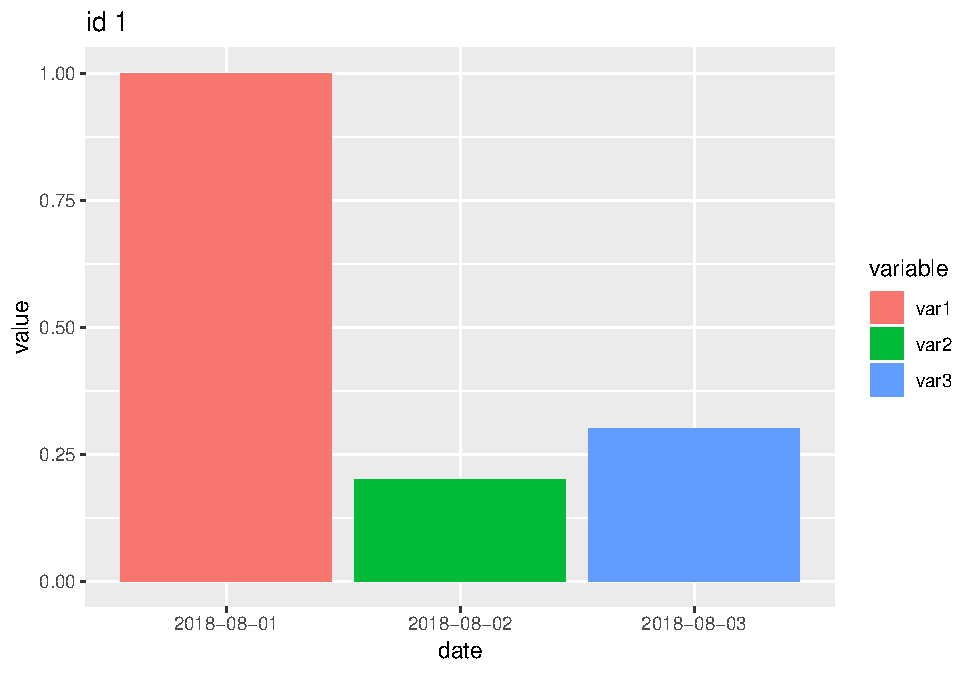
\includegraphics{modern_R_files/figure-latex/unnamed-chunk-219-1.pdf}

Ok great. But now I want to create this plot for each
\texttt{id}\ldots{} so I have to copy paste this 3 times. But
copy-pasting is error prone. So there are two alternatives; I either
write a function that takes as argument the data and the \texttt{id}
I~want to plot and run it for each \texttt{id} (we will learn to do this
in Chapter 8), or I can use \texttt{tidyr::nest()}, combined with
\texttt{purrr::map()}. \texttt{\{purrr\}} is another very useful
\texttt{\{tidevyrse\}} package, and we are going to learn about it in
Chapter 9. Again, just follow along for now:

\begin{Shaded}
\begin{Highlighting}[]
\NormalTok{my_plots <-}\StringTok{ }\NormalTok{nested_survey_data }\OperatorTok
\StringTok{    }\KeywordTok{mutate}\NormalTok{(}\DataTypeTok{plot =} \KeywordTok{map2}\NormalTok{(}\DataTypeTok{.x =}\NormalTok{ id,}
                       \DataTypeTok{.y =}\NormalTok{ data,}
                       \OperatorTok{~}\KeywordTok{ggplot}\NormalTok{(}\DataTypeTok{data =}\NormalTok{ .y) }\OperatorTok{+}
\StringTok{                           }\KeywordTok{geom_bar}\NormalTok{(}\KeywordTok{aes}\NormalTok{(}\DataTypeTok{y =}\NormalTok{ value, }\DataTypeTok{x =}\NormalTok{ date, }\DataTypeTok{fill =}\NormalTok{ variable), }\DataTypeTok{stat =} \StringTok{"identity"}\NormalTok{) }\OperatorTok{+}
\StringTok{                           }\KeywordTok{ggtitle}\NormalTok{(}\KeywordTok{paste0}\NormalTok{(}\StringTok{"id"}\NormalTok{, .x))))}
\end{Highlighting}
\end{Shaded}

This is some very advanced stuff, and again, do not worry if you don't
understand everything now. We are going to learn about this in detail in
Chapter 9. Let's go through each line. In the first line, I have started
from my clean data \texttt{nested\_survey\_data} and then, using the
\texttt{\%\textgreater{}\%} and \texttt{mutate()} I create a new column
called \texttt{plot}. Inside the \texttt{mutate()} function, I called
\texttt{map2}. \texttt{map2} is a \texttt{\{purrr\}} function that takes
three inputs: \texttt{.x}, \texttt{.y} and a function. \texttt{.x} is
the \texttt{id} column from my data, and \texttt{.y} is the
\texttt{data} column from \texttt{nested\_survey\_data}. The function is
the ggplot I created before. Think of \texttt{map2()} has a loop over
two lists, all while applying a function.

The following illustration, taken from \citet{vaudor_purrr_2018} by
\href{https://twitter.com/LVaudor}{Lise Vaudor}, illustrates this
perfectly:

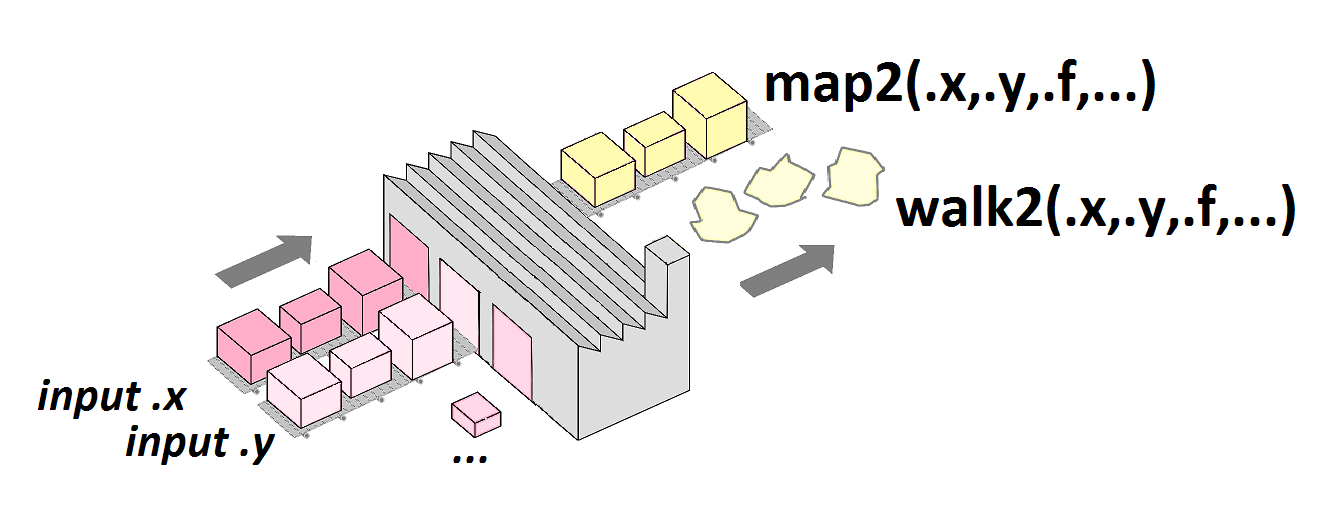
\includegraphics[width=18.42in]{assets/purrr3}

Two inputs go in at the same type, the factory, your function, does what
it has to do, and an output comes out. Forget about the factory's
chimney, which represents \texttt{walk2()} for now. We'll learn about it
in due time. By the way, you really should read Lise's blog, her posts
are really great and informative. It's in French, but that's not a
problem, you know how to read R code, right? Here's a link to
\href{http://perso.ens-lyon.fr/lise.vaudor/}{her blog}.

Now, let's take a look at the result:

\begin{Shaded}
\begin{Highlighting}[]
\NormalTok{my_plots}
\end{Highlighting}
\end{Shaded}

\begin{verbatim}
## # A tibble: 4 x 3
##      id data             plot    
##   <dbl> <list>           <list>  
## 1     1 <tibble [3 x 3]> <S3: gg>
## 2     2 <tibble [3 x 3]> <S3: gg>
## 3     3 <tibble [3 x 3]> <S3: gg>
## 4     4 <tibble [3 x 3]> <S3: gg>
\end{verbatim}

\texttt{my\_plots} is a tibble with three columns: \texttt{id},
\texttt{data} and.. \texttt{plot}! \texttt{plot} is a very interesting
column. It is a list, where each element is of type \texttt{S3:\ gg}.
Yes, you guessed it, each element of that list-column is a ggplot! If
you now want to take a look at the plots, it is enough to do this:

\begin{Shaded}
\begin{Highlighting}[]
\NormalTok{my_plots}\OperatorTok{$}\NormalTok{plot}
\end{Highlighting}
\end{Shaded}

\begin{verbatim}
## [[1]]
\end{verbatim}

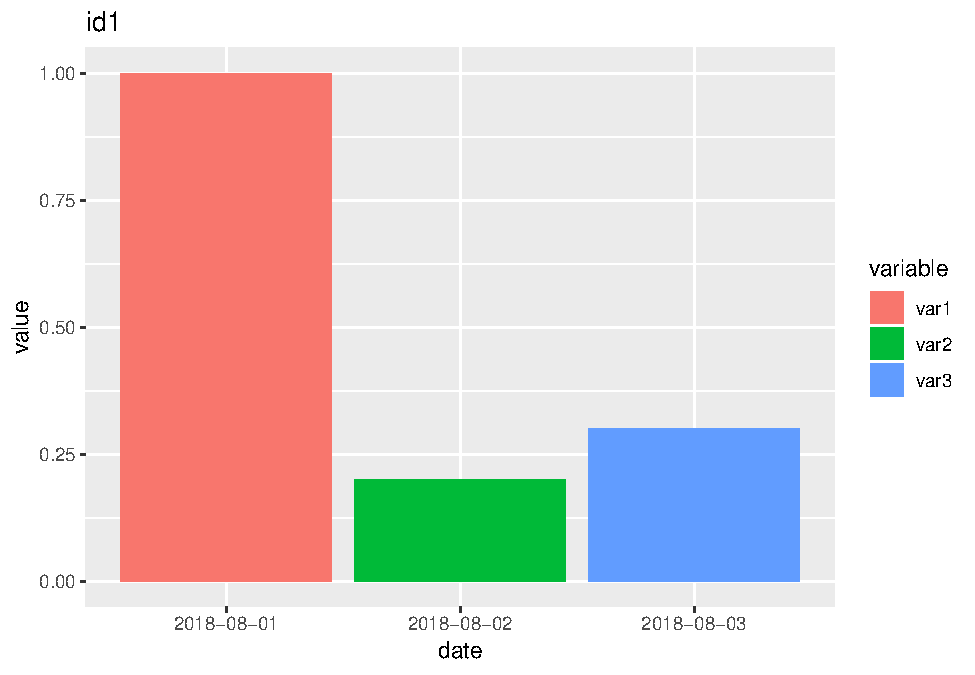
\includegraphics{modern_R_files/figure-latex/unnamed-chunk-223-1.pdf}

\begin{verbatim}
## 
## [[2]]
\end{verbatim}

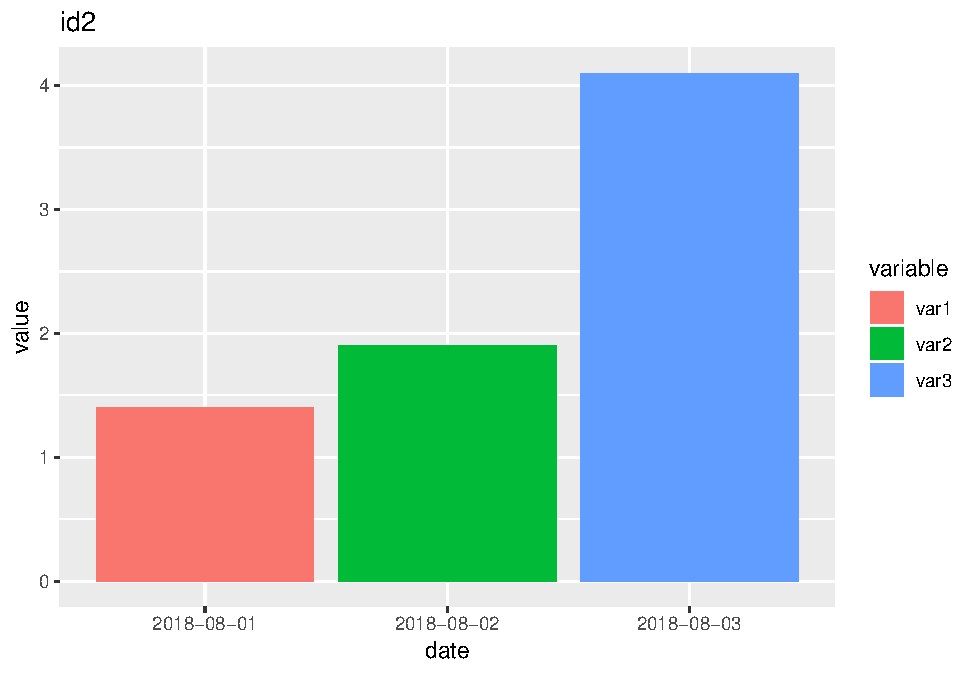
\includegraphics{modern_R_files/figure-latex/unnamed-chunk-223-2.pdf}

\begin{verbatim}
## 
## [[3]]
\end{verbatim}

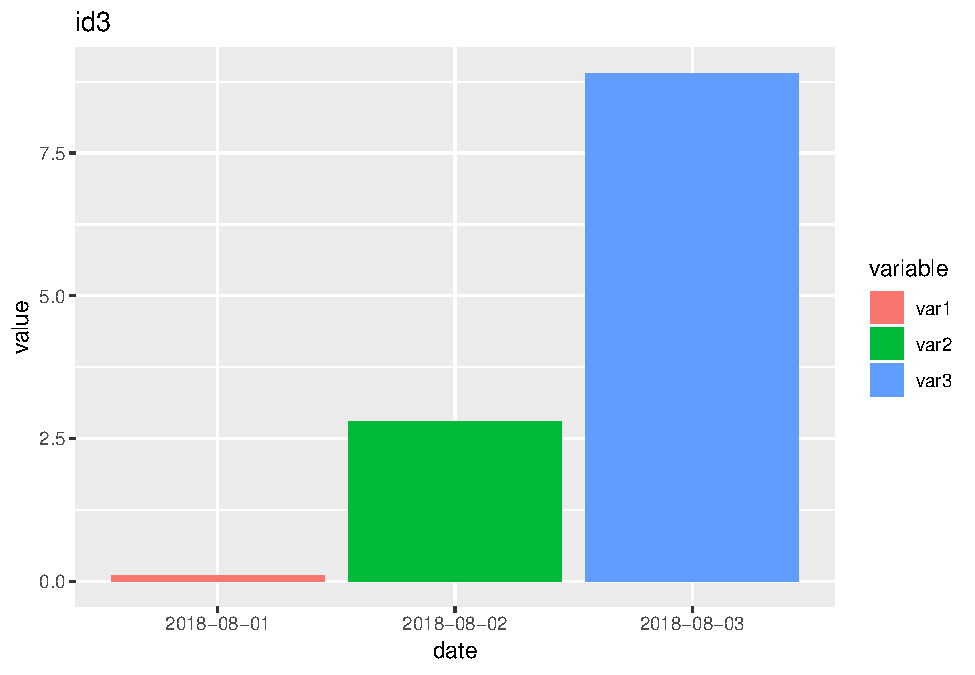
\includegraphics{modern_R_files/figure-latex/unnamed-chunk-223-3.pdf}

\begin{verbatim}
## 
## [[4]]
\end{verbatim}

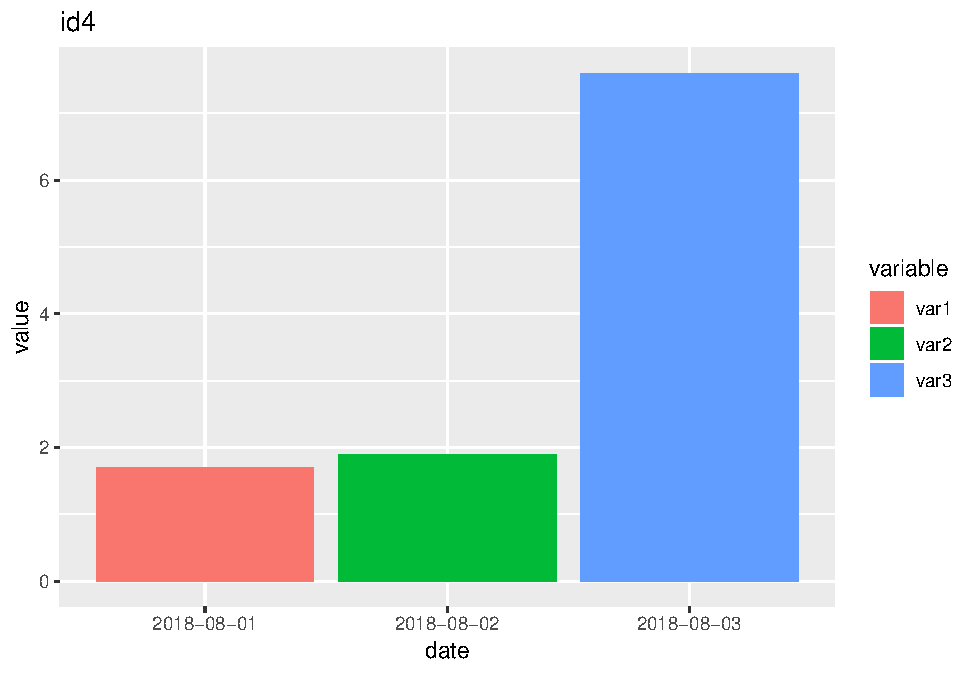
\includegraphics{modern_R_files/figure-latex/unnamed-chunk-223-4.pdf}

Ok, that was quite complicated, but again, this was only to introduce
\texttt{nest()} and give you a taste of the power of the
\texttt{\{tidyverse\}}. By the end of Chapter 9, you'll be used to this.

That was it for a first introduction to \texttt{\{tidyr\}}. Now, it's
time to learn about \emph{scoped} verbs.

\hypertarget{scoped-tidyverse-verbs}{%
\subsection{\texorpdfstring{Scoped \texttt{\{tidyverse\}}
verbs}{Scoped \{tidyverse\} verbs}}\label{scoped-tidyverse-verbs}}

Scoped verbs are special versions of the verbs you are now familiar
with.

\hypertarget{filter_}{%
\subsubsection{filter\_*()}\label{filter_}}

Let's go back to the \texttt{gasoline} data from the \texttt{\{plm\}}
package.

\texttt{filter()} is not the only \emph{filtering} verb there is.
Suppose that we have a condition that we want to use to filter out a lot
of columns at once. For example, for every column that is of type
\texttt{numeric}, keep only the lines where the condition \emph{value
\textgreater{} -8} is satisfied. The next line does that:

\begin{Shaded}
\begin{Highlighting}[]
\NormalTok{gasoline }\OperatorTok\StringTok{ }\KeywordTok{filter_if}\NormalTok{( }\OperatorTok{~}\KeywordTok{all}\NormalTok{(}\KeywordTok{is.numeric}\NormalTok{(.)), }\KeywordTok{all_vars}\NormalTok{(. }\OperatorTok{>}\StringTok{ }\DecValTok{-8}\NormalTok{))}
\end{Highlighting}
\end{Shaded}

\begin{verbatim}
## # A tibble: 30 x 6
##    country  year lgaspcar lincomep  lrpmg lcarpcap
##    <fct>   <int>    <dbl>    <dbl>  <dbl>    <dbl>
##  1 CANADA   1972     4.89    -5.44 -1.10     -7.99
##  2 CANADA   1973     4.90    -5.41 -1.13     -7.94
##  3 CANADA   1974     4.89    -5.42 -1.12     -7.90
##  4 CANADA   1975     4.89    -5.38 -1.19     -7.87
##  5 CANADA   1976     4.84    -5.36 -1.06     -7.81
##  6 CANADA   1977     4.81    -5.34 -1.07     -7.77
##  7 CANADA   1978     4.86    -5.31 -1.07     -7.79
##  8 GERMANY  1978     3.88    -5.56 -0.628    -7.95
##  9 SWEDEN   1975     3.97    -7.68 -2.77     -7.99
## 10 SWEDEN   1976     3.98    -7.67 -2.82     -7.96
## # ... with 20 more rows
\end{verbatim}

This is a bit more complicated than before, but let's go through it,
step by step. \texttt{filter\_if()} needs 3 arguments to work; the data,
a predicate function (a function that returns \texttt{TRUE}, or
\texttt{FALSE}) which will select the columns we want to work on, and
then the condition. The condition can be applied to \emph{all} the
columns that were selected by the predicate function (hence the
\texttt{all\_vars()}) or only to at least one (you'd use
\texttt{any\_vars()} then). Try to change the condition, or the
predicate function, to figure out how \texttt{filter\_if()} works. The
dot is a placeholder that stands for whatever columns where selected.

Another scoped \texttt{filter()} verb is \texttt{filter\_at()}; it
allows the user to filter columns by position:

\begin{Shaded}
\begin{Highlighting}[]
\NormalTok{gasoline }\OperatorTok\StringTok{ }\KeywordTok{filter_at}\NormalTok{(}\KeywordTok{vars}\NormalTok{(}\KeywordTok{ends_with}\NormalTok{(}\StringTok{"p"}\NormalTok{)), }\KeywordTok{all_vars}\NormalTok{(. }\OperatorTok{>}\StringTok{ }\DecValTok{-8}\NormalTok{))}
\end{Highlighting}
\end{Shaded}

\begin{verbatim}
## # A tibble: 30 x 6
##    country  year lgaspcar lincomep  lrpmg lcarpcap
##    <fct>   <int>    <dbl>    <dbl>  <dbl>    <dbl>
##  1 CANADA   1972     4.89    -5.44 -1.10     -7.99
##  2 CANADA   1973     4.90    -5.41 -1.13     -7.94
##  3 CANADA   1974     4.89    -5.42 -1.12     -7.90
##  4 CANADA   1975     4.89    -5.38 -1.19     -7.87
##  5 CANADA   1976     4.84    -5.36 -1.06     -7.81
##  6 CANADA   1977     4.81    -5.34 -1.07     -7.77
##  7 CANADA   1978     4.86    -5.31 -1.07     -7.79
##  8 GERMANY  1978     3.88    -5.56 -0.628    -7.95
##  9 SWEDEN   1975     3.97    -7.68 -2.77     -7.99
## 10 SWEDEN   1976     3.98    -7.67 -2.82     -7.96
## # ... with 20 more rows
\end{verbatim}

we already know about \texttt{ends\_with()} and \texttt{starts\_with()}.
So the above line means ``for the columns whose name end with a `p' only
keep the lines where, for all the selected columns, the values are
strictly superior to \texttt{-8}''. Again, this is not very easy the
first time you deal with that, so play around with it for a bit.

Finally, there is also \texttt{filter\_all()} which, as the name
implies, uses all the variables for the filtering step.

\texttt{filter\_if()} and \texttt{filter\_at()} are very useful when you
have very large datasets with a lot of variables and you want to apply a
filtering function only to a subset of them. \texttt{filter\_all()} is
useful if, for example, you only want to keep the positive values for
all the columns.

\hypertarget{select_-and-rename_}{%
\subsubsection{select\_*() and rename\_*()}\label{select_-and-rename_}}

Just as with \texttt{filter()}, \texttt{select()} also has scoped
versions. \texttt{select\_if()} makes it easy to select columns that
satisfy a criterium:

\begin{Shaded}
\begin{Highlighting}[]
\NormalTok{gasoline }\OperatorTok\StringTok{ }\KeywordTok{select_if}\NormalTok{(is.numeric)}
\end{Highlighting}
\end{Shaded}

\begin{verbatim}
## # A tibble: 342 x 5
##     year lgaspcar lincomep  lrpmg lcarpcap
##  * <int>    <dbl>    <dbl>  <dbl>    <dbl>
##  1  1960     4.17    -6.47 -0.335    -9.77
##  2  1961     4.10    -6.43 -0.351    -9.61
##  3  1962     4.07    -6.41 -0.380    -9.46
##  4  1963     4.06    -6.37 -0.414    -9.34
##  5  1964     4.04    -6.32 -0.445    -9.24
##  6  1965     4.03    -6.29 -0.497    -9.12
##  7  1966     4.05    -6.25 -0.467    -9.02
##  8  1967     4.05    -6.23 -0.506    -8.93
##  9  1968     4.05    -6.21 -0.522    -8.85
## 10  1969     4.05    -6.15 -0.559    -8.79
## # ... with 332 more rows
\end{verbatim}

You can even pass a further function to \texttt{select\_if()} that will
be applied to the selected columns:

\begin{Shaded}
\begin{Highlighting}[]
\NormalTok{gasoline }\OperatorTok\StringTok{ }\KeywordTok{select_if}\NormalTok{(is.numeric, toupper)}
\end{Highlighting}
\end{Shaded}

\begin{verbatim}
## # A tibble: 342 x 5
##     YEAR LGASPCAR LINCOMEP  LRPMG LCARPCAP
##  * <int>    <dbl>    <dbl>  <dbl>    <dbl>
##  1  1960     4.17    -6.47 -0.335    -9.77
##  2  1961     4.10    -6.43 -0.351    -9.61
##  3  1962     4.07    -6.41 -0.380    -9.46
##  4  1963     4.06    -6.37 -0.414    -9.34
##  5  1964     4.04    -6.32 -0.445    -9.24
##  6  1965     4.03    -6.29 -0.497    -9.12
##  7  1966     4.05    -6.25 -0.467    -9.02
##  8  1967     4.05    -6.23 -0.506    -8.93
##  9  1968     4.05    -6.21 -0.522    -8.85
## 10  1969     4.05    -6.15 -0.559    -8.79
## # ... with 332 more rows
\end{verbatim}

\texttt{select\_at()} makes it easy to select all the variables that
start with ``l'' for example:

\begin{Shaded}
\begin{Highlighting}[]
\NormalTok{gasoline }\OperatorTok\StringTok{ }\KeywordTok{select_at}\NormalTok{(}\KeywordTok{vars}\NormalTok{(}\KeywordTok{starts_with}\NormalTok{(}\StringTok{"l"}\NormalTok{)))}
\end{Highlighting}
\end{Shaded}

\begin{verbatim}
## # A tibble: 342 x 4
##    lgaspcar lincomep  lrpmg lcarpcap
##  *    <dbl>    <dbl>  <dbl>    <dbl>
##  1     4.17    -6.47 -0.335    -9.77
##  2     4.10    -6.43 -0.351    -9.61
##  3     4.07    -6.41 -0.380    -9.46
##  4     4.06    -6.37 -0.414    -9.34
##  5     4.04    -6.32 -0.445    -9.24
##  6     4.03    -6.29 -0.497    -9.12
##  7     4.05    -6.25 -0.467    -9.02
##  8     4.05    -6.23 -0.506    -8.93
##  9     4.05    -6.21 -0.522    -8.85
## 10     4.05    -6.15 -0.559    -8.79
## # ... with 332 more rows
\end{verbatim}

\texttt{select\_at()} also works if you specify the position of the
columns you're interested in:

\begin{Shaded}
\begin{Highlighting}[]
\NormalTok{gasoline }\OperatorTok\StringTok{ }\KeywordTok{select_at}\NormalTok{(}\KeywordTok{vars}\NormalTok{(}\KeywordTok{c}\NormalTok{(}\DecValTok{1}\NormalTok{,}\DecValTok{2}\NormalTok{,}\DecValTok{5}\NormalTok{)))}
\end{Highlighting}
\end{Shaded}

\begin{verbatim}
## # A tibble: 342 x 3
##    country  year  lrpmg
##  * <fct>   <int>  <dbl>
##  1 AUSTRIA  1960 -0.335
##  2 AUSTRIA  1961 -0.351
##  3 AUSTRIA  1962 -0.380
##  4 AUSTRIA  1963 -0.414
##  5 AUSTRIA  1964 -0.445
##  6 AUSTRIA  1965 -0.497
##  7 AUSTRIA  1966 -0.467
##  8 AUSTRIA  1967 -0.506
##  9 AUSTRIA  1968 -0.522
## 10 AUSTRIA  1969 -0.559
## # ... with 332 more rows
\end{verbatim}

Notice that I use a new helper function, \texttt{vars()}, which allows
me to specify which variables I want to select. This is similar to the
helper functions we have seen before, \texttt{all\_vars()} and
\texttt{any\_vars()}. So the way to read the above line would be
something like ``Start with the gasoline data, then select the variables
at position 1, 2, 5''. Knowing how to read your code makes it even
easier to write.

There is also a \texttt{select\_all()}, and you might be wondering why
it is useful:

\begin{Shaded}
\begin{Highlighting}[]
\NormalTok{gasoline }\OperatorTok\StringTok{ }\KeywordTok{select_all}\NormalTok{()}
\end{Highlighting}
\end{Shaded}

\begin{verbatim}
## # A tibble: 342 x 6
##    country  year lgaspcar lincomep  lrpmg lcarpcap
##  * <fct>   <int>    <dbl>    <dbl>  <dbl>    <dbl>
##  1 AUSTRIA  1960     4.17    -6.47 -0.335    -9.77
##  2 AUSTRIA  1961     4.10    -6.43 -0.351    -9.61
##  3 AUSTRIA  1962     4.07    -6.41 -0.380    -9.46
##  4 AUSTRIA  1963     4.06    -6.37 -0.414    -9.34
##  5 AUSTRIA  1964     4.04    -6.32 -0.445    -9.24
##  6 AUSTRIA  1965     4.03    -6.29 -0.497    -9.12
##  7 AUSTRIA  1966     4.05    -6.25 -0.467    -9.02
##  8 AUSTRIA  1967     4.05    -6.23 -0.506    -8.93
##  9 AUSTRIA  1968     4.05    -6.21 -0.522    -8.85
## 10 AUSTRIA  1969     4.05    -6.15 -0.559    -8.79
## # ... with 332 more rows
\end{verbatim}

This simply returns all the columns of the data frame\ldots{} but wait,
\texttt{selec\_all()} allows you to do something very useful, which is
rename all the columns in bulk:

\begin{Shaded}
\begin{Highlighting}[]
\NormalTok{gasoline }\OperatorTok\StringTok{ }\KeywordTok{select_all}\NormalTok{(toupper)}
\end{Highlighting}
\end{Shaded}

\begin{verbatim}
## # A tibble: 342 x 6
##    COUNTRY  YEAR LGASPCAR LINCOMEP  LRPMG LCARPCAP
##  * <fct>   <int>    <dbl>    <dbl>  <dbl>    <dbl>
##  1 AUSTRIA  1960     4.17    -6.47 -0.335    -9.77
##  2 AUSTRIA  1961     4.10    -6.43 -0.351    -9.61
##  3 AUSTRIA  1962     4.07    -6.41 -0.380    -9.46
##  4 AUSTRIA  1963     4.06    -6.37 -0.414    -9.34
##  5 AUSTRIA  1964     4.04    -6.32 -0.445    -9.24
##  6 AUSTRIA  1965     4.03    -6.29 -0.497    -9.12
##  7 AUSTRIA  1966     4.05    -6.25 -0.467    -9.02
##  8 AUSTRIA  1967     4.05    -6.23 -0.506    -8.93
##  9 AUSTRIA  1968     4.05    -6.21 -0.522    -8.85
## 10 AUSTRIA  1969     4.05    -6.15 -0.559    -8.79
## # ... with 332 more rows
\end{verbatim}

You can apply any arbitrary function:

\begin{Shaded}
\begin{Highlighting}[]
\NormalTok{gasoline }\OperatorTok\StringTok{ }\KeywordTok{select_all}\NormalTok{(}\KeywordTok{funs}\NormalTok{(}\KeywordTok{paste0}\NormalTok{(}\StringTok{"hello_"}\NormalTok{, .)))}
\end{Highlighting}
\end{Shaded}

\begin{verbatim}
## # A tibble: 342 x 6
##    hello_country hello_year hello_lgaspcar hello_lincomep hello_lrpmg
##  * <fct>              <int>          <dbl>          <dbl>       <dbl>
##  1 AUSTRIA             1960           4.17          -6.47      -0.335
##  2 AUSTRIA             1961           4.10          -6.43      -0.351
##  3 AUSTRIA             1962           4.07          -6.41      -0.380
##  4 AUSTRIA             1963           4.06          -6.37      -0.414
##  5 AUSTRIA             1964           4.04          -6.32      -0.445
##  6 AUSTRIA             1965           4.03          -6.29      -0.497
##  7 AUSTRIA             1966           4.05          -6.25      -0.467
##  8 AUSTRIA             1967           4.05          -6.23      -0.506
##  9 AUSTRIA             1968           4.05          -6.21      -0.522
## 10 AUSTRIA             1969           4.05          -6.15      -0.559
## # ... with 332 more rows, and 1 more variable: hello_lcarpcap <dbl>
\end{verbatim}

I have passed the \texttt{paste0()} function to the \texttt{funs()}
helper function of \texttt{select\_all()}. \texttt{funs()} is used a lot
with scoped verbs, just like \texttt{vars()}, which we have already
seen.

The scoped version of \texttt{rename()} work just as you expect. But
I'll leave these for the exercices down below.

\hypertarget{group_by_}{%
\subsubsection{group\_by\_*()}\label{group_by_}}

To illustrate \texttt{group\_by\_*()} I have to first modify the
\texttt{gasoline} data a little bit. As you can see below, the data
column is of type integer:

\begin{Shaded}
\begin{Highlighting}[]
\NormalTok{gasoline}
\end{Highlighting}
\end{Shaded}

\begin{verbatim}
## # A tibble: 342 x 6
##    country  year lgaspcar lincomep  lrpmg lcarpcap
##  * <fct>   <int>    <dbl>    <dbl>  <dbl>    <dbl>
##  1 AUSTRIA  1960     4.17    -6.47 -0.335    -9.77
##  2 AUSTRIA  1961     4.10    -6.43 -0.351    -9.61
##  3 AUSTRIA  1962     4.07    -6.41 -0.380    -9.46
##  4 AUSTRIA  1963     4.06    -6.37 -0.414    -9.34
##  5 AUSTRIA  1964     4.04    -6.32 -0.445    -9.24
##  6 AUSTRIA  1965     4.03    -6.29 -0.497    -9.12
##  7 AUSTRIA  1966     4.05    -6.25 -0.467    -9.02
##  8 AUSTRIA  1967     4.05    -6.23 -0.506    -8.93
##  9 AUSTRIA  1968     4.05    -6.21 -0.522    -8.85
## 10 AUSTRIA  1969     4.05    -6.15 -0.559    -8.79
## # ... with 332 more rows
\end{verbatim}

Let's change that to character:

\begin{Shaded}
\begin{Highlighting}[]
\NormalTok{gasoline <-}\StringTok{ }\NormalTok{gasoline }\OperatorTok
\StringTok{    }\KeywordTok{mutate}\NormalTok{(}\DataTypeTok{year =} \KeywordTok{as.character}\NormalTok{(year))}
\end{Highlighting}
\end{Shaded}

Now, this allows me to do the following:

\begin{Shaded}
\begin{Highlighting}[]
\NormalTok{gasoline }\OperatorTok
\StringTok{    }\KeywordTok{group_by_if}\NormalTok{(is.character) }\OperatorTok
\StringTok{    }\KeywordTok{summarise}\NormalTok{(}\KeywordTok{mean}\NormalTok{(lincomep))}
\end{Highlighting}
\end{Shaded}

\begin{verbatim}
## # A tibble: 19 x 2
##    year  `mean(lincomep)`
##    <chr>            <dbl>
##  1 1960             -6.50
##  2 1961             -6.46
##  3 1962             -6.42
##  4 1963             -6.37
##  5 1964             -6.33
##  6 1965             -6.29
##  7 1966             -6.25
##  8 1967             -6.21
##  9 1968             -6.18
## 10 1969             -6.12
## 11 1970             -6.07
## 12 1971             -6.04
## 13 1972             -5.99
## 14 1973             -5.94
## 15 1974             -5.93
## 16 1975             -5.93
## 17 1976             -5.89
## 18 1977             -5.87
## 19 1978             -5.84
\end{verbatim}

This is faster than having to write:

\begin{Shaded}
\begin{Highlighting}[]
\NormalTok{gasoline }\OperatorTok
\StringTok{    }\KeywordTok{group_by}\NormalTok{(country, year) }\OperatorTok
\StringTok{    }\KeywordTok{summarise}\NormalTok{(}\KeywordTok{mean}\NormalTok{(lincomep))}
\end{Highlighting}
\end{Shaded}

\begin{verbatim}
## # A tibble: 342 x 3
## # Groups:   country [?]
##    country year  `mean(lincomep)`
##    <fct>   <chr>            <dbl>
##  1 AUSTRIA 1960             -6.47
##  2 AUSTRIA 1961             -6.43
##  3 AUSTRIA 1962             -6.41
##  4 AUSTRIA 1963             -6.37
##  5 AUSTRIA 1964             -6.32
##  6 AUSTRIA 1965             -6.29
##  7 AUSTRIA 1966             -6.25
##  8 AUSTRIA 1967             -6.23
##  9 AUSTRIA 1968             -6.21
## 10 AUSTRIA 1969             -6.15
## # ... with 332 more rows
\end{verbatim}

You may think that having two write the name of two variables is not a
huge hassle, which is true. But imagine that you have dozens of
character columns that you want to group by. This is the kind of
situation where \texttt{group\_by\_if()} is very useful. If you prefer,
you can specify the position of the columns instead of the name of the
columns, with \texttt{group\_by\_at()}:

\begin{Shaded}
\begin{Highlighting}[]
\NormalTok{gasoline }\OperatorTok
\StringTok{    }\KeywordTok{group_by_at}\NormalTok{(}\KeywordTok{vars}\NormalTok{(}\DecValTok{1}\NormalTok{, }\DecValTok{2}\NormalTok{)) }\OperatorTok
\StringTok{    }\KeywordTok{summarise}\NormalTok{(}\KeywordTok{mean}\NormalTok{(lincomep))}
\end{Highlighting}
\end{Shaded}

\begin{verbatim}
## # A tibble: 342 x 3
## # Groups:   country [?]
##    country year  `mean(lincomep)`
##    <fct>   <chr>            <dbl>
##  1 AUSTRIA 1960             -6.47
##  2 AUSTRIA 1961             -6.43
##  3 AUSTRIA 1962             -6.41
##  4 AUSTRIA 1963             -6.37
##  5 AUSTRIA 1964             -6.32
##  6 AUSTRIA 1965             -6.29
##  7 AUSTRIA 1966             -6.25
##  8 AUSTRIA 1967             -6.23
##  9 AUSTRIA 1968             -6.21
## 10 AUSTRIA 1969             -6.15
## # ... with 332 more rows
\end{verbatim}

There is also a \texttt{group\_by\_all()}, but I fail to see the use
case\ldots{}

\hypertarget{summarise_}{%
\subsubsection{summarise\_()}\label{summarise_}}

Just like for \texttt{filter()}, \texttt{select()}, and
\texttt{group\_by()}, summarise()` comes with scoped versions:

\begin{Shaded}
\begin{Highlighting}[]
\NormalTok{gasoline }\OperatorTok
\StringTok{  }\KeywordTok{group_by}\NormalTok{(country) }\OperatorTok
\StringTok{  }\KeywordTok{summarise_at}\NormalTok{(}\KeywordTok{vars}\NormalTok{(}\KeywordTok{starts_with}\NormalTok{(}\StringTok{"l"}\NormalTok{)), mean)}
\end{Highlighting}
\end{Shaded}

\begin{verbatim}
## # A tibble: 18 x 5
##    country  lgaspcar lincomep   lrpmg lcarpcap
##    <fct>       <dbl>    <dbl>   <dbl>    <dbl>
##  1 AUSTRIA      4.06    -6.12 -0.486     -8.85
##  2 BELGIUM      3.92    -5.85 -0.326     -8.63
##  3 CANADA       4.86    -5.58 -1.05      -8.08
##  4 DENMARK      4.19    -5.76 -0.358     -8.58
##  5 FRANCE       3.82    -5.87 -0.253     -8.45
##  6 GERMANY      3.89    -5.85 -0.517     -8.51
##  7 GREECE       4.88    -6.61 -0.0339   -10.8 
##  8 IRELAND      4.23    -6.44 -0.348     -9.04
##  9 ITALY        3.73    -6.35 -0.152     -8.83
## 10 JAPAN        4.70    -6.25 -0.287     -9.95
## 11 NETHERLA     4.08    -5.92 -0.370     -8.82
## 12 NORWAY       4.11    -5.75 -0.278     -8.77
## 13 SPAIN        4.06    -5.63  0.739     -9.90
## 14 SWEDEN       4.01    -7.82 -2.71      -8.25
## 15 SWITZERL     4.24    -5.93 -0.902     -8.54
## 16 TURKEY       5.77    -7.34 -0.422    -12.5 
## 17 U.K.         3.98    -6.02 -0.459     -8.55
## 18 U.S.A.       4.82    -5.45 -1.21      -7.78
\end{verbatim}

See how I managed to summarise every variable in one simple call to
\texttt{summarise\_at()}? Simply by using \texttt{vars()} and specifying
that I was interested in the ones that started with ``l'' and then I
specified the function I wanted. But what if I wanted to use more than
one function to summarise the data? Very easy:

\begin{Shaded}
\begin{Highlighting}[]
\NormalTok{gasoline }\OperatorTok
\StringTok{  }\KeywordTok{group_by}\NormalTok{(country) }\OperatorTok
\StringTok{  }\KeywordTok{summarise_at}\NormalTok{(}\KeywordTok{vars}\NormalTok{(}\KeywordTok{starts_with}\NormalTok{(}\StringTok{"l"}\NormalTok{)), }\KeywordTok{funs}\NormalTok{(mean, sd, max, min))}
\end{Highlighting}
\end{Shaded}

\begin{verbatim}
## # A tibble: 18 x 17
##    country lgaspcar_mean lincomep_mean lrpmg_mean lcarpcap_mean lgaspcar_sd
##    <fct>           <dbl>         <dbl>      <dbl>         <dbl>       <dbl>
##  1 AUSTRIA          4.06         -6.12    -0.486          -8.85      0.0693
##  2 BELGIUM          3.92         -5.85    -0.326          -8.63      0.103 
##  3 CANADA           4.86         -5.58    -1.05           -8.08      0.0262
##  4 DENMARK          4.19         -5.76    -0.358          -8.58      0.158 
##  5 FRANCE           3.82         -5.87    -0.253          -8.45      0.0499
##  6 GERMANY          3.89         -5.85    -0.517          -8.51      0.0239
##  7 GREECE           4.88         -6.61    -0.0339        -10.8       0.255 
##  8 IRELAND          4.23         -6.44    -0.348          -9.04      0.0437
##  9 ITALY            3.73         -6.35    -0.152          -8.83      0.220 
## 10 JAPAN            4.70         -6.25    -0.287          -9.95      0.684 
## 11 NETHER~          4.08         -5.92    -0.370          -8.82      0.286 
## 12 NORWAY           4.11         -5.75    -0.278          -8.77      0.123 
## 13 SPAIN            4.06         -5.63     0.739          -9.90      0.317 
## 14 SWEDEN           4.01         -7.82    -2.71           -8.25      0.0364
## 15 SWITZE~          4.24         -5.93    -0.902          -8.54      0.102 
## 16 TURKEY           5.77         -7.34    -0.422         -12.5       0.329 
## 17 U.K.             3.98         -6.02    -0.459          -8.55      0.0479
## 18 U.S.A.           4.82         -5.45    -1.21           -7.78      0.0219
## # ... with 11 more variables: lincomep_sd <dbl>, lrpmg_sd <dbl>,
## #   lcarpcap_sd <dbl>, lgaspcar_max <dbl>, lincomep_max <dbl>,
## #   lrpmg_max <dbl>, lcarpcap_max <dbl>, lgaspcar_min <dbl>,
## #   lincomep_min <dbl>, lrpmg_min <dbl>, lcarpcap_min <dbl>
\end{verbatim}

Just use \texttt{vars()} to specify the variables you want to summarise,
and then \texttt{funs()} to list all the functions you want to use on
each of the columns.

But maybe you're just interested in descriptive statistics for some
variables, but not all those that start with ``l''? What if you want to
use another pattern? Easy to do with the \texttt{contains()} helper:

\begin{Shaded}
\begin{Highlighting}[]
\NormalTok{gasoline }\OperatorTok
\StringTok{  }\KeywordTok{group_by}\NormalTok{(country) }\OperatorTok
\StringTok{  }\KeywordTok{summarise_at}\NormalTok{(}\KeywordTok{vars}\NormalTok{(dplyr}\OperatorTok{::}\KeywordTok{contains}\NormalTok{(}\StringTok{"car"}\NormalTok{)), }\KeywordTok{funs}\NormalTok{(mean, sd, max, min))}
\end{Highlighting}
\end{Shaded}

\begin{verbatim}
## # A tibble: 18 x 9
##    country lgaspcar_mean lcarpcap_mean lgaspcar_sd lcarpcap_sd lgaspcar_max
##    <fct>           <dbl>         <dbl>       <dbl>       <dbl>        <dbl>
##  1 AUSTRIA          4.06         -8.85      0.0693       0.473         4.20
##  2 BELGIUM          3.92         -8.63      0.103        0.417         4.16
##  3 CANADA           4.86         -8.08      0.0262       0.195         4.90
##  4 DENMARK          4.19         -8.58      0.158        0.349         4.50
##  5 FRANCE           3.82         -8.45      0.0499       0.344         3.91
##  6 GERMANY          3.89         -8.51      0.0239       0.406         3.93
##  7 GREECE           4.88        -10.8       0.255        0.839         5.38
##  8 IRELAND          4.23         -9.04      0.0437       0.345         4.33
##  9 ITALY            3.73         -8.83      0.220        0.639         4.05
## 10 JAPAN            4.70         -9.95      0.684        1.20          6.00
## 11 NETHER~          4.08         -8.82      0.286        0.617         4.65
## 12 NORWAY           4.11         -8.77      0.123        0.438         4.44
## 13 SPAIN            4.06         -9.90      0.317        0.960         4.75
## 14 SWEDEN           4.01         -8.25      0.0364       0.242         4.07
## 15 SWITZE~          4.24         -8.54      0.102        0.378         4.44
## 16 TURKEY           5.77        -12.5       0.329        0.751         6.16
## 17 U.K.             3.98         -8.55      0.0479       0.281         4.10
## 18 U.S.A.           4.82         -7.78      0.0219       0.162         4.86
## # ... with 3 more variables: lcarpcap_max <dbl>, lgaspcar_min <dbl>,
## #   lcarpcap_min <dbl>
\end{verbatim}

I used \texttt{dplyr::contains()} instead of simply \texttt{contains()}
because there's also a \texttt{purrr::contains()}. If you load
\texttt{purrr} after \texttt{dplyr}, \texttt{contains()} will actually
be \texttt{purrr::contains()} and not \texttt{dplyr::contains()} which
causes the above code to fail.

There's also \texttt{summarise\_if()}:

\begin{Shaded}
\begin{Highlighting}[]
\NormalTok{gasoline }\OperatorTok
\StringTok{  }\KeywordTok{group_by}\NormalTok{(country) }\OperatorTok
\StringTok{  }\KeywordTok{summarise_if}\NormalTok{(is.double, }\KeywordTok{funs}\NormalTok{(mean, sd, min, max))}
\end{Highlighting}
\end{Shaded}

\begin{verbatim}
## # A tibble: 18 x 17
##    country lgaspcar_mean lincomep_mean lrpmg_mean lcarpcap_mean lgaspcar_sd
##    <fct>           <dbl>         <dbl>      <dbl>         <dbl>       <dbl>
##  1 AUSTRIA          4.06         -6.12    -0.486          -8.85      0.0693
##  2 BELGIUM          3.92         -5.85    -0.326          -8.63      0.103 
##  3 CANADA           4.86         -5.58    -1.05           -8.08      0.0262
##  4 DENMARK          4.19         -5.76    -0.358          -8.58      0.158 
##  5 FRANCE           3.82         -5.87    -0.253          -8.45      0.0499
##  6 GERMANY          3.89         -5.85    -0.517          -8.51      0.0239
##  7 GREECE           4.88         -6.61    -0.0339        -10.8       0.255 
##  8 IRELAND          4.23         -6.44    -0.348          -9.04      0.0437
##  9 ITALY            3.73         -6.35    -0.152          -8.83      0.220 
## 10 JAPAN            4.70         -6.25    -0.287          -9.95      0.684 
## 11 NETHER~          4.08         -5.92    -0.370          -8.82      0.286 
## 12 NORWAY           4.11         -5.75    -0.278          -8.77      0.123 
## 13 SPAIN            4.06         -5.63     0.739          -9.90      0.317 
## 14 SWEDEN           4.01         -7.82    -2.71           -8.25      0.0364
## 15 SWITZE~          4.24         -5.93    -0.902          -8.54      0.102 
## 16 TURKEY           5.77         -7.34    -0.422         -12.5       0.329 
## 17 U.K.             3.98         -6.02    -0.459          -8.55      0.0479
## 18 U.S.A.           4.82         -5.45    -1.21           -7.78      0.0219
## # ... with 11 more variables: lincomep_sd <dbl>, lrpmg_sd <dbl>,
## #   lcarpcap_sd <dbl>, lgaspcar_min <dbl>, lincomep_min <dbl>,
## #   lrpmg_min <dbl>, lcarpcap_min <dbl>, lgaspcar_max <dbl>,
## #   lincomep_max <dbl>, lrpmg_max <dbl>, lcarpcap_max <dbl>
\end{verbatim}

This allows you to summarise every column that contain real numbers. The
difference between \texttt{is.double()} and \texttt{is.numeric()} is
that \texttt{is.numeric()} returns \texttt{TRUE} for integers too,
whereas \texttt{is.double()} returns \texttt{TRUE} for real numbers only
(integers are real numbers too, but you know what I mean). To go faster,
you can also use \texttt{summarise\_all()}:

\begin{Shaded}
\begin{Highlighting}[]
\NormalTok{gasoline }\OperatorTok
\StringTok{  }\KeywordTok{select}\NormalTok{(}\OperatorTok{-}\NormalTok{year) }\OperatorTok
\StringTok{  }\KeywordTok{group_by}\NormalTok{(country) }\OperatorTok
\StringTok{  }\KeywordTok{summarise_all}\NormalTok{(}\KeywordTok{funs}\NormalTok{(mean, sd, min, max))}
\end{Highlighting}
\end{Shaded}

\begin{verbatim}
## # A tibble: 18 x 17
##    country lgaspcar_mean lincomep_mean lrpmg_mean lcarpcap_mean lgaspcar_sd
##    <fct>           <dbl>         <dbl>      <dbl>         <dbl>       <dbl>
##  1 AUSTRIA          4.06         -6.12    -0.486          -8.85      0.0693
##  2 BELGIUM          3.92         -5.85    -0.326          -8.63      0.103 
##  3 CANADA           4.86         -5.58    -1.05           -8.08      0.0262
##  4 DENMARK          4.19         -5.76    -0.358          -8.58      0.158 
##  5 FRANCE           3.82         -5.87    -0.253          -8.45      0.0499
##  6 GERMANY          3.89         -5.85    -0.517          -8.51      0.0239
##  7 GREECE           4.88         -6.61    -0.0339        -10.8       0.255 
##  8 IRELAND          4.23         -6.44    -0.348          -9.04      0.0437
##  9 ITALY            3.73         -6.35    -0.152          -8.83      0.220 
## 10 JAPAN            4.70         -6.25    -0.287          -9.95      0.684 
## 11 NETHER~          4.08         -5.92    -0.370          -8.82      0.286 
## 12 NORWAY           4.11         -5.75    -0.278          -8.77      0.123 
## 13 SPAIN            4.06         -5.63     0.739          -9.90      0.317 
## 14 SWEDEN           4.01         -7.82    -2.71           -8.25      0.0364
## 15 SWITZE~          4.24         -5.93    -0.902          -8.54      0.102 
## 16 TURKEY           5.77         -7.34    -0.422         -12.5       0.329 
## 17 U.K.             3.98         -6.02    -0.459          -8.55      0.0479
## 18 U.S.A.           4.82         -5.45    -1.21           -7.78      0.0219
## # ... with 11 more variables: lincomep_sd <dbl>, lrpmg_sd <dbl>,
## #   lcarpcap_sd <dbl>, lgaspcar_min <dbl>, lincomep_min <dbl>,
## #   lrpmg_min <dbl>, lcarpcap_min <dbl>, lgaspcar_max <dbl>,
## #   lincomep_max <dbl>, lrpmg_max <dbl>, lcarpcap_max <dbl>
\end{verbatim}

I removed the \texttt{year} variable because it's not a variable for
which we want to have descriptive statistics.

\hypertarget{mutate_}{%
\subsubsection{mutate\_*()}\label{mutate_}}

Of course, \texttt{mutate()} and \texttt{transmute()} also come with
scoped versions:

\begin{Shaded}
\begin{Highlighting}[]
\NormalTok{gasoline }\OperatorTok
\StringTok{  }\KeywordTok{mutate_if}\NormalTok{(is.double, exp)}
\end{Highlighting}
\end{Shaded}

\begin{verbatim}
## # A tibble: 342 x 6
##    country year  lgaspcar lincomep lrpmg  lcarpcap
##    <fct>   <chr>    <dbl>    <dbl> <dbl>     <dbl>
##  1 AUSTRIA 1960      64.9  0.00154 0.716 0.0000573
##  2 AUSTRIA 1961      60.4  0.00162 0.704 0.0000671
##  3 AUSTRIA 1962      58.7  0.00165 0.684 0.0000781
##  4 AUSTRIA 1963      57.9  0.00171 0.661 0.0000876
##  5 AUSTRIA 1964      56.7  0.00180 0.641 0.0000973
##  6 AUSTRIA 1965      56.5  0.00185 0.608 0.000109 
##  7 AUSTRIA 1966      57.3  0.00193 0.627 0.000121 
##  8 AUSTRIA 1967      57.6  0.00196 0.603 0.000132 
##  9 AUSTRIA 1968      57.1  0.00202 0.593 0.000144 
## 10 AUSTRIA 1969      57.2  0.00213 0.572 0.000152 
## # ... with 332 more rows
\end{verbatim}

\begin{Shaded}
\begin{Highlighting}[]
\NormalTok{gasoline }\OperatorTok
\StringTok{  }\KeywordTok{mutate_at}\NormalTok{(}\KeywordTok{vars}\NormalTok{(}\KeywordTok{starts_with}\NormalTok{(}\StringTok{"l"}\NormalTok{)), exp)}
\end{Highlighting}
\end{Shaded}

\begin{verbatim}
## # A tibble: 342 x 6
##    country year  lgaspcar lincomep lrpmg  lcarpcap
##    <fct>   <chr>    <dbl>    <dbl> <dbl>     <dbl>
##  1 AUSTRIA 1960      64.9  0.00154 0.716 0.0000573
##  2 AUSTRIA 1961      60.4  0.00162 0.704 0.0000671
##  3 AUSTRIA 1962      58.7  0.00165 0.684 0.0000781
##  4 AUSTRIA 1963      57.9  0.00171 0.661 0.0000876
##  5 AUSTRIA 1964      56.7  0.00180 0.641 0.0000973
##  6 AUSTRIA 1965      56.5  0.00185 0.608 0.000109 
##  7 AUSTRIA 1966      57.3  0.00193 0.627 0.000121 
##  8 AUSTRIA 1967      57.6  0.00196 0.603 0.000132 
##  9 AUSTRIA 1968      57.1  0.00202 0.593 0.000144 
## 10 AUSTRIA 1969      57.2  0.00213 0.572 0.000152 
## # ... with 332 more rows
\end{verbatim}

\begin{Shaded}
\begin{Highlighting}[]
\NormalTok{gasoline }\OperatorTok
\StringTok{  }\KeywordTok{mutate_all}\NormalTok{(as.character)}
\end{Highlighting}
\end{Shaded}

\begin{verbatim}
## # A tibble: 342 x 6
##    country year  lgaspcar     lincomep     lrpmg        lcarpcap    
##    <chr>   <chr> <chr>        <chr>        <chr>        <chr>       
##  1 AUSTRIA 1960  4.173244195  -6.474277179 -0.334547613 -9.766839569
##  2 AUSTRIA 1961  4.1009891049 -6.426005835 -0.351327614 -9.608621845
##  3 AUSTRIA 1962  4.0731765511 -6.407308295 -0.379517692 -9.457256552
##  4 AUSTRIA 1963  4.0595091239 -6.370678539 -0.414251392 -9.343154947
##  5 AUSTRIA 1964  4.037688787  -6.322246805 -0.445335362 -9.237739346
##  6 AUSTRIA 1965  4.033983285  -6.294667914 -0.497060662 -9.123903477
##  7 AUSTRIA 1966  4.0475365589 -6.252545451 -0.466837731 -9.019822048
##  8 AUSTRIA 1967  4.0529106939 -6.234580709 -0.505883405 -8.934402537
##  9 AUSTRIA 1968  4.045507048  -6.206894403 -0.522412545 -8.847967407
## 10 AUSTRIA 1969  4.0463547891 -6.153139668 -0.559110514 -8.788686207
## # ... with 332 more rows
\end{verbatim}

I think that by now, you are able to understand the above lines quite
easily. If not, try some other functions, or mutating other variables
and you'll see that it is not that complicated!

\hypertarget{other-useful-tidyverse-functions}{%
\subsection{\texorpdfstring{Other useful \texttt{\{tidyverse\}}
functions}{Other useful \{tidyverse\} functions}}\label{other-useful-tidyverse-functions}}

\hypertarget{if_else-case_when-and-recode}{%
\subsubsection{\texorpdfstring{\texttt{if\_else()},
\texttt{case\_when()} and
\texttt{recode()}}{if\_else(), case\_when() and recode()}}\label{if_else-case_when-and-recode}}

Some other very useful \texttt{\{tidyverse\}} functions are
\texttt{if\_else()} and \texttt{case\_when}. These two functions,
combined with \texttt{mutate()} make it easy to create a new variable
whose values must respect certain conditions. For instance, we might
want to have a dummy that equals \texttt{1} if a country in the European
Union (to simplify, say as of 2017) and \texttt{0} if not. First let's
create a list of countries that are in the EU:

\begin{Shaded}
\begin{Highlighting}[]
\NormalTok{eu_countries <-}\StringTok{ }\KeywordTok{c}\NormalTok{(}\StringTok{"austria"}\NormalTok{, }\StringTok{"belgium"}\NormalTok{, }\StringTok{"bulgaria"}\NormalTok{, }\StringTok{"croatia"}\NormalTok{, }\StringTok{"republic of cyprus"}\NormalTok{,}
                  \StringTok{"czech republic"}\NormalTok{, }\StringTok{"denmark"}\NormalTok{, }\StringTok{"estonia"}\NormalTok{, }\StringTok{"finland"}\NormalTok{, }\StringTok{"france"}\NormalTok{, }\StringTok{"germany"}\NormalTok{,}
                  \StringTok{"greece"}\NormalTok{, }\StringTok{"hungary"}\NormalTok{, }\StringTok{"ireland"}\NormalTok{, }\StringTok{"italy"}\NormalTok{, }\StringTok{"latvia"}\NormalTok{, }\StringTok{"lithuania"}\NormalTok{, }\StringTok{"luxembourg"}\NormalTok{,}
                  \StringTok{"malta"}\NormalTok{, }\StringTok{"netherla"}\NormalTok{, }\StringTok{"poland"}\NormalTok{, }\StringTok{"portugal"}\NormalTok{, }\StringTok{"romania"}\NormalTok{, }\StringTok{"slovakia"}\NormalTok{, }\StringTok{"slovenia"}\NormalTok{,}
                  \StringTok{"spain"}\NormalTok{, }\StringTok{"sweden"}\NormalTok{, }\StringTok{"u.k."}\NormalTok{)}
\end{Highlighting}
\end{Shaded}

I've had to change ``netherlands'' to ``netherla'' because that's how
the country is called in the \texttt{gasoline} data. Now let's create a
dummy variable that equals \texttt{1} for EU countries, and \texttt{0}
for the others:

\begin{Shaded}
\begin{Highlighting}[]
\NormalTok{gasoline }\OperatorTok
\StringTok{  }\KeywordTok{mutate}\NormalTok{(}\DataTypeTok{country =} \KeywordTok{tolower}\NormalTok{(country)) }\OperatorTok
\StringTok{  }\KeywordTok{mutate}\NormalTok{(}\DataTypeTok{in_eu =} \KeywordTok{if_else}\NormalTok{(country }\OperatorTok\StringTok{ }\NormalTok{eu_countries, }\DecValTok{1}\NormalTok{, }\DecValTok{0}\NormalTok{))}
\end{Highlighting}
\end{Shaded}

\begin{verbatim}
## # A tibble: 342 x 7
##    country  year lgaspcar lincomep  lrpmg lcarpcap in_eu
##    <chr>   <dbl>    <dbl>    <dbl>  <dbl>    <dbl> <dbl>
##  1 austria  1960     4.17    -6.47 -0.335    -9.77     1
##  2 austria  1961     4.10    -6.43 -0.351    -9.61     1
##  3 austria  1962     4.07    -6.41 -0.380    -9.46     1
##  4 austria  1963     4.06    -6.37 -0.414    -9.34     1
##  5 austria  1964     4.04    -6.32 -0.445    -9.24     1
##  6 austria  1965     4.03    -6.29 -0.497    -9.12     1
##  7 austria  1966     4.05    -6.25 -0.467    -9.02     1
##  8 austria  1967     4.05    -6.23 -0.506    -8.93     1
##  9 austria  1968     4.05    -6.21 -0.522    -8.85     1
## 10 austria  1969     4.05    -6.15 -0.559    -8.79     1
## # ... with 332 more rows
\end{verbatim}

Instead of \texttt{1} and \texttt{0}, we can of course use strings (I
add \texttt{filter(year\ ==\ 1960)} at the end to have a better view of
what happened):

\begin{Shaded}
\begin{Highlighting}[]
\NormalTok{gasoline }\OperatorTok
\StringTok{  }\KeywordTok{mutate}\NormalTok{(}\DataTypeTok{country =} \KeywordTok{tolower}\NormalTok{(country)) }\OperatorTok
\StringTok{  }\KeywordTok{mutate}\NormalTok{(}\DataTypeTok{in_eu =} \KeywordTok{if_else}\NormalTok{(country }\OperatorTok\StringTok{ }\NormalTok{eu_countries, }\StringTok{"yes"}\NormalTok{, }\StringTok{"no"}\NormalTok{)) }\OperatorTok
\StringTok{  }\KeywordTok{filter}\NormalTok{(year }\OperatorTok{==}\StringTok{ }\DecValTok{1960}\NormalTok{)}
\end{Highlighting}
\end{Shaded}

\begin{verbatim}
## # A tibble: 18 x 7
##    country   year lgaspcar lincomep   lrpmg lcarpcap in_eu
##    <chr>    <dbl>    <dbl>    <dbl>   <dbl>    <dbl> <chr>
##  1 austria   1960     4.17    -6.47 -0.335     -9.77 yes  
##  2 belgium   1960     4.16    -6.22 -0.166     -9.41 yes  
##  3 canada    1960     4.86    -5.89 -0.972     -8.38 no   
##  4 denmark   1960     4.50    -6.06 -0.196     -9.33 yes  
##  5 france    1960     3.91    -6.26 -0.0196    -9.15 yes  
##  6 germany   1960     3.92    -6.16 -0.186     -9.34 yes  
##  7 greece    1960     5.04    -7.16 -0.0835   -12.2  yes  
##  8 ireland   1960     4.27    -6.72 -0.0765    -9.70 yes  
##  9 italy     1960     4.05    -6.73  0.165    -10.1  yes  
## 10 japan     1960     6.00    -6.99 -0.145    -12.2  no   
## 11 netherla  1960     4.65    -6.22 -0.201    -10.00 yes  
## 12 norway    1960     4.44    -6.09 -0.140     -9.68 no   
## 13 spain     1960     4.75    -6.17  1.13     -11.6  yes  
## 14 sweden    1960     4.06    -8.07 -2.52      -8.74 yes  
## 15 switzerl  1960     4.40    -6.16 -0.823     -9.26 no   
## 16 turkey    1960     6.13    -7.80 -0.253    -13.5  no   
## 17 u.k.      1960     4.10    -6.19 -0.391     -9.12 yes  
## 18 u.s.a.    1960     4.82    -5.70 -1.12      -8.02 no
\end{verbatim}

I think that \texttt{if\_else()} is fairly straightforward, especially
if you know \texttt{ifelse()} already. You might be wondering what is
the difference between these two. \texttt{if\_else()} is stricter than
\texttt{ifelse()} and does not do type conversion. Compare the two next
lines:

\begin{Shaded}
\begin{Highlighting}[]
\KeywordTok{ifelse}\NormalTok{(}\DecValTok{1} \OperatorTok{==}\StringTok{ }\DecValTok{1}\NormalTok{, }\StringTok{"0"}\NormalTok{, }\DecValTok{1}\NormalTok{)}
\end{Highlighting}
\end{Shaded}

\begin{verbatim}
## [1] "0"
\end{verbatim}

\begin{Shaded}
\begin{Highlighting}[]
\KeywordTok{if_else}\NormalTok{(}\DecValTok{1} \OperatorTok{==}\StringTok{ }\DecValTok{1}\NormalTok{, }\StringTok{"0"}\NormalTok{, }\DecValTok{1}\NormalTok{)}
\end{Highlighting}
\end{Shaded}

\begin{Shaded}
\begin{Highlighting}[]
\NormalTok{Error}\OperatorTok{:}\StringTok{ `}\DataTypeTok{false}\StringTok{`}\NormalTok{ must be type string, not double}
\end{Highlighting}
\end{Shaded}

Type conversion, especially without a warning is very dangerous.
\texttt{if\_else()}'s behaviour which consists in failing as soon as
possble avoids a lot of pain and suffering, especially when programming
non-interactively.

\texttt{if\_else()} also accepts an optional argument, that allows you
to specify what should be returned in case of \texttt{NA}:

\begin{Shaded}
\begin{Highlighting}[]
\KeywordTok{if_else}\NormalTok{(}\DecValTok{1} \OperatorTok{<=}\StringTok{ }\OtherTok{NA}\NormalTok{, }\DecValTok{0}\NormalTok{, }\DecValTok{1}\NormalTok{, }\DecValTok{999}\NormalTok{)}
\end{Highlighting}
\end{Shaded}

\begin{verbatim}
## [1] 999
\end{verbatim}

\begin{Shaded}
\begin{Highlighting}[]
\CommentTok{# Or}
\KeywordTok{if_else}\NormalTok{(}\DecValTok{1} \OperatorTok{<=}\StringTok{ }\OtherTok{NA}\NormalTok{, }\DecValTok{0}\NormalTok{, }\DecValTok{1}\NormalTok{, }\OtherTok{NA_real_}\NormalTok{)}
\end{Highlighting}
\end{Shaded}

\begin{verbatim}
## [1] NA
\end{verbatim}

\texttt{case\_when()} can be seen as a generalization of
\texttt{if\_else()}. Whenever you want to use multiple
\texttt{if\_else()}s, that's when you know you should use
\texttt{case\_when()} (I'm adding the filter at the end for the same
reason as before, to see the output better):

\begin{Shaded}
\begin{Highlighting}[]
\NormalTok{gasoline }\OperatorTok
\StringTok{  }\KeywordTok{mutate}\NormalTok{(}\DataTypeTok{country =} \KeywordTok{tolower}\NormalTok{(country)) }\OperatorTok
\StringTok{  }\KeywordTok{mutate}\NormalTok{(}\DataTypeTok{region =} \KeywordTok{case_when}\NormalTok{(}
\NormalTok{           country }\OperatorTok\StringTok{ }\KeywordTok{c}\NormalTok{(}\StringTok{"france"}\NormalTok{, }\StringTok{"italy"}\NormalTok{, }\StringTok{"turkey"}\NormalTok{, }\StringTok{"greece"}\NormalTok{, }\StringTok{"spain"}\NormalTok{) }\OperatorTok{~}\StringTok{ "mediterranean"}\NormalTok{,}
\NormalTok{           country }\OperatorTok\StringTok{ }\KeywordTok{c}\NormalTok{(}\StringTok{"germany"}\NormalTok{, }\StringTok{"austria"}\NormalTok{, }\StringTok{"switzerl"}\NormalTok{, }\StringTok{"belgium"}\NormalTok{, }\StringTok{"netherla"}\NormalTok{) }\OperatorTok{~}\StringTok{ "central europe"}\NormalTok{,}
\NormalTok{           country }\OperatorTok\StringTok{ }\KeywordTok{c}\NormalTok{(}\StringTok{"canada"}\NormalTok{, }\StringTok{"u.s.a."}\NormalTok{, }\StringTok{"u.k."}\NormalTok{, }\StringTok{"ireland"}\NormalTok{) }\OperatorTok{~}\StringTok{ "anglosphere"}\NormalTok{,}
\NormalTok{           country }\OperatorTok\StringTok{ }\KeywordTok{c}\NormalTok{(}\StringTok{"denmark"}\NormalTok{, }\StringTok{"norway"}\NormalTok{, }\StringTok{"sweden"}\NormalTok{) }\OperatorTok{~}\StringTok{ "nordic"}\NormalTok{,}
\NormalTok{           country }\OperatorTok\StringTok{ }\KeywordTok{c}\NormalTok{(}\StringTok{"japan"}\NormalTok{) }\OperatorTok{~}\StringTok{ "asia"}\NormalTok{)) }\OperatorTok
\StringTok{  }\KeywordTok{filter}\NormalTok{(year }\OperatorTok{==}\StringTok{ }\DecValTok{1960}\NormalTok{)}
\end{Highlighting}
\end{Shaded}

\begin{verbatim}
## # A tibble: 18 x 7
##    country   year lgaspcar lincomep   lrpmg lcarpcap region        
##    <chr>    <dbl>    <dbl>    <dbl>   <dbl>    <dbl> <chr>         
##  1 austria   1960     4.17    -6.47 -0.335     -9.77 central europe
##  2 belgium   1960     4.16    -6.22 -0.166     -9.41 central europe
##  3 canada    1960     4.86    -5.89 -0.972     -8.38 anglosphere   
##  4 denmark   1960     4.50    -6.06 -0.196     -9.33 nordic        
##  5 france    1960     3.91    -6.26 -0.0196    -9.15 mediterranean 
##  6 germany   1960     3.92    -6.16 -0.186     -9.34 central europe
##  7 greece    1960     5.04    -7.16 -0.0835   -12.2  mediterranean 
##  8 ireland   1960     4.27    -6.72 -0.0765    -9.70 anglosphere   
##  9 italy     1960     4.05    -6.73  0.165    -10.1  mediterranean 
## 10 japan     1960     6.00    -6.99 -0.145    -12.2  asia          
## 11 netherla  1960     4.65    -6.22 -0.201    -10.00 central europe
## 12 norway    1960     4.44    -6.09 -0.140     -9.68 nordic        
## 13 spain     1960     4.75    -6.17  1.13     -11.6  mediterranean 
## 14 sweden    1960     4.06    -8.07 -2.52      -8.74 nordic        
## 15 switzerl  1960     4.40    -6.16 -0.823     -9.26 central europe
## 16 turkey    1960     6.13    -7.80 -0.253    -13.5  mediterranean 
## 17 u.k.      1960     4.10    -6.19 -0.391     -9.12 anglosphere   
## 18 u.s.a.    1960     4.82    -5.70 -1.12      -8.02 anglosphere
\end{verbatim}

If all you want is to recode values, you can use \texttt{recode()}. For
example, the Netherlands is written as ``NETHERLA'' in the
\texttt{gasoline} data, which is quite ugly. Same for Switzerland:

\begin{Shaded}
\begin{Highlighting}[]
\NormalTok{gasoline <-}\StringTok{ }\NormalTok{gasoline }\OperatorTok
\StringTok{  }\KeywordTok{mutate}\NormalTok{(}\DataTypeTok{country =} \KeywordTok{tolower}\NormalTok{(country)) }\OperatorTok
\StringTok{  }\KeywordTok{mutate}\NormalTok{(}\DataTypeTok{country =} \KeywordTok{recode}\NormalTok{(country, }\StringTok{"netherla"}\NormalTok{ =}\StringTok{ "netherlands"}\NormalTok{, }\StringTok{"switzerl"}\NormalTok{ =}\StringTok{ "switzerland"}\NormalTok{))}
\end{Highlighting}
\end{Shaded}

I saved the data with these changes as they will become useful in the
future. Let's take a look at the data:

\begin{Shaded}
\begin{Highlighting}[]
\NormalTok{gasoline }\OperatorTok
\StringTok{  }\KeywordTok{filter}\NormalTok{(country }\OperatorTok\StringTok{ }\KeywordTok{c}\NormalTok{(}\StringTok{"netherlands"}\NormalTok{, }\StringTok{"switzerland"}\NormalTok{), year }\OperatorTok{==}\StringTok{ }\DecValTok{1960}\NormalTok{)}
\end{Highlighting}
\end{Shaded}

\begin{verbatim}
## # A tibble: 2 x 6
##   country      year lgaspcar lincomep  lrpmg lcarpcap
##   <chr>       <dbl>    <dbl>    <dbl>  <dbl>    <dbl>
## 1 netherlands  1960     4.65    -6.22 -0.201   -10.00
## 2 switzerland  1960     4.40    -6.16 -0.823    -9.26
\end{verbatim}

\hypertarget{lead-and-lag}{%
\subsubsection{\texorpdfstring{\texttt{lead()} and
\texttt{lag()}}{lead() and lag()}}\label{lead-and-lag}}

\texttt{lead()} and \texttt{lag()} are especially useful in
econometrics. When I was doing my masters, in 4 B.d. (\emph{Before
dplyr}) lagging variables in panel data was quite tricky. Now, with
\texttt{dplyr} it's really very easy:

\begin{Shaded}
\begin{Highlighting}[]
\NormalTok{gasoline }\OperatorTok
\StringTok{  }\KeywordTok{group_by}\NormalTok{(country) }\OperatorTok
\StringTok{  }\KeywordTok{mutate}\NormalTok{(}\DataTypeTok{lag_lgaspcar =} \KeywordTok{lag}\NormalTok{(lgaspcar)) }\OperatorTok
\StringTok{  }\KeywordTok{mutate}\NormalTok{(}\DataTypeTok{lead_lgaspcar =} \KeywordTok{lead}\NormalTok{(lgaspcar)) }\OperatorTok
\StringTok{  }\KeywordTok{filter}\NormalTok{(year }\OperatorTok\StringTok{ }\KeywordTok{seq}\NormalTok{(}\DecValTok{1960}\NormalTok{, }\DecValTok{1963}\NormalTok{))}
\end{Highlighting}
\end{Shaded}

\begin{verbatim}
## # A tibble: 72 x 8
## # Groups:   country [18]
##    country  year lgaspcar lincomep  lrpmg lcarpcap lag_lgaspcar
##    <chr>   <dbl>    <dbl>    <dbl>  <dbl>    <dbl>        <dbl>
##  1 austria  1960     4.17    -6.47 -0.335    -9.77        NA   
##  2 austria  1961     4.10    -6.43 -0.351    -9.61         4.17
##  3 austria  1962     4.07    -6.41 -0.380    -9.46         4.10
##  4 austria  1963     4.06    -6.37 -0.414    -9.34         4.07
##  5 belgium  1960     4.16    -6.22 -0.166    -9.41        NA   
##  6 belgium  1961     4.12    -6.18 -0.172    -9.30         4.16
##  7 belgium  1962     4.08    -6.13 -0.222    -9.22         4.12
##  8 belgium  1963     4.00    -6.09 -0.250    -9.11         4.08
##  9 canada   1960     4.86    -5.89 -0.972    -8.38        NA   
## 10 canada   1961     4.83    -5.88 -0.972    -8.35         4.86
## # ... with 62 more rows, and 1 more variable: lead_lgaspcar <dbl>
\end{verbatim}

To lag every variable, remember that you can use \texttt{mutate\_if()}:

\begin{Shaded}
\begin{Highlighting}[]
\NormalTok{gasoline }\OperatorTok
\StringTok{  }\KeywordTok{group_by}\NormalTok{(country) }\OperatorTok
\StringTok{  }\KeywordTok{mutate_if}\NormalTok{(is.double, lag) }\OperatorTok
\StringTok{  }\KeywordTok{filter}\NormalTok{(year }\OperatorTok\StringTok{ }\KeywordTok{seq}\NormalTok{(}\DecValTok{1960}\NormalTok{, }\DecValTok{1963}\NormalTok{))}
\end{Highlighting}
\end{Shaded}

\begin{verbatim}
## # A tibble: 72 x 6
## # Groups:   country [18]
##    country  year lgaspcar lincomep  lrpmg lcarpcap
##    <chr>   <dbl>    <dbl>    <dbl>  <dbl>    <dbl>
##  1 austria  1960     4.17    -6.47 -0.335    -9.77
##  2 austria  1961     4.10    -6.43 -0.351    -9.61
##  3 austria  1962     4.07    -6.41 -0.380    -9.46
##  4 austria  1963     4.06    -6.37 -0.414    -9.34
##  5 belgium  1960     4.16    -6.22 -0.166    -9.41
##  6 belgium  1961     4.12    -6.18 -0.172    -9.30
##  7 belgium  1962     4.08    -6.13 -0.222    -9.22
##  8 belgium  1963     4.00    -6.09 -0.250    -9.11
##  9 canada   1960     4.86    -5.89 -0.972    -8.38
## 10 canada   1961     4.83    -5.88 -0.972    -8.35
## # ... with 62 more rows
\end{verbatim}

you can replace \texttt{lag()} with \texttt{lead()}, but just keep in
mind that the columns get transformed in place.

\hypertarget{ntile}{%
\subsubsection{\texorpdfstring{\texttt{ntile()}}{ntile()}}\label{ntile}}

The last helper function I will discuss is \texttt{ntile()}. There are
some other, so do read \texttt{mutate()}'s documentation with
\texttt{help(mutate)}!

If you need quantiles, you need \texttt{ntile()}. Let's see how it
works:

\begin{Shaded}
\begin{Highlighting}[]
\NormalTok{gasoline }\OperatorTok
\StringTok{  }\KeywordTok{mutate}\NormalTok{(}\DataTypeTok{quintile =} \KeywordTok{ntile}\NormalTok{(lgaspcar, }\DecValTok{5}\NormalTok{)) }\OperatorTok
\StringTok{  }\KeywordTok{mutate}\NormalTok{(}\DataTypeTok{decile =} \KeywordTok{ntile}\NormalTok{(lgaspcar, }\DecValTok{10}\NormalTok{)) }\OperatorTok
\StringTok{  }\KeywordTok{select}\NormalTok{(country, year, lgaspcar, quintile, decile)}
\end{Highlighting}
\end{Shaded}

\begin{verbatim}
## # A tibble: 342 x 5
##    country  year lgaspcar quintile decile
##    <chr>   <dbl>    <dbl>    <int>  <int>
##  1 austria  1960     4.17        3      6
##  2 austria  1961     4.10        3      6
##  3 austria  1962     4.07        3      5
##  4 austria  1963     4.06        3      5
##  5 austria  1964     4.04        3      5
##  6 austria  1965     4.03        3      5
##  7 austria  1966     4.05        3      5
##  8 austria  1967     4.05        3      5
##  9 austria  1968     4.05        3      5
## 10 austria  1969     4.05        3      5
## # ... with 332 more rows
\end{verbatim}

\texttt{quintile} and \texttt{decile} do not hold the values but the
quantile the value lies in. If you want to have a column that contains
the median for instance, you can use good ol' \texttt{quantile()}:

\begin{Shaded}
\begin{Highlighting}[]
\NormalTok{gasoline }\OperatorTok
\StringTok{  }\KeywordTok{group_by}\NormalTok{(country) }\OperatorTok
\StringTok{  }\KeywordTok{mutate}\NormalTok{(}\DataTypeTok{median =} \KeywordTok{quantile}\NormalTok{(lgaspcar, }\FloatTok{0.5}\NormalTok{)) }\OperatorTok\StringTok{ }\CommentTok{# quantile(x, 0.5) is equivalent to median(x)}
\StringTok{  }\KeywordTok{filter}\NormalTok{(year }\OperatorTok{==}\StringTok{ }\DecValTok{1960}\NormalTok{) }\OperatorTok
\StringTok{  }\KeywordTok{select}\NormalTok{(country, year, median)}
\end{Highlighting}
\end{Shaded}

\begin{verbatim}
## # A tibble: 18 x 3
## # Groups:   country [18]
##    country      year median
##    <chr>       <dbl>  <dbl>
##  1 austria      1960   4.05
##  2 belgium      1960   3.88
##  3 canada       1960   4.86
##  4 denmark      1960   4.16
##  5 france       1960   3.81
##  6 germany      1960   3.89
##  7 greece       1960   4.89
##  8 ireland      1960   4.22
##  9 italy        1960   3.74
## 10 japan        1960   4.52
## 11 netherlands  1960   3.99
## 12 norway       1960   4.08
## 13 spain        1960   3.99
## 14 sweden       1960   4.00
## 15 switzerland  1960   4.26
## 16 turkey       1960   5.72
## 17 u.k.         1960   3.98
## 18 u.s.a.       1960   4.81
\end{verbatim}

\hypertarget{arrange}{%
\subsubsection{\texorpdfstring{\texttt{arrange()}}{arrange()}}\label{arrange}}

\texttt{arrange()} re-orders the whole \texttt{tibble} according to
values of the supplied variable:

\begin{Shaded}
\begin{Highlighting}[]
\NormalTok{gasoline }\OperatorTok
\StringTok{  }\KeywordTok{arrange}\NormalTok{(lgaspcar)}
\end{Highlighting}
\end{Shaded}

\begin{verbatim}
## # A tibble: 342 x 6
##    country  year lgaspcar lincomep   lrpmg lcarpcap
##    <chr>   <dbl>    <dbl>    <dbl>   <dbl>    <dbl>
##  1 italy    1977     3.38    -6.10  0.164     -8.15
##  2 italy    1978     3.39    -6.08  0.0348    -8.11
##  3 italy    1976     3.43    -6.12  0.103     -8.17
##  4 italy    1974     3.50    -6.13 -0.223     -8.26
##  5 italy    1975     3.52    -6.17 -0.0327    -8.22
##  6 spain    1978     3.62    -5.29  0.621     -8.63
##  7 italy    1972     3.63    -6.21 -0.215     -8.38
##  8 italy    1971     3.65    -6.22 -0.148     -8.47
##  9 spain    1977     3.65    -5.30  0.526     -8.73
## 10 italy    1973     3.65    -6.16 -0.325     -8.32
## # ... with 332 more rows
\end{verbatim}

If you want to re-order the \texttt{tibble} in descending order of the
variable:

\begin{Shaded}
\begin{Highlighting}[]
\NormalTok{gasoline }\OperatorTok
\StringTok{  }\KeywordTok{arrange}\NormalTok{(}\KeywordTok{desc}\NormalTok{(lgaspcar))}
\end{Highlighting}
\end{Shaded}

\begin{verbatim}
## # A tibble: 342 x 6
##    country  year lgaspcar lincomep  lrpmg lcarpcap
##    <chr>   <dbl>    <dbl>    <dbl>  <dbl>    <dbl>
##  1 turkey   1966     6.16    -7.51 -0.356    -13.0
##  2 turkey   1960     6.13    -7.80 -0.253    -13.5
##  3 turkey   1961     6.11    -7.79 -0.343    -13.4
##  4 turkey   1962     6.08    -7.84 -0.408    -13.2
##  5 turkey   1968     6.08    -7.42 -0.365    -12.8
##  6 turkey   1963     6.08    -7.63 -0.225    -13.3
##  7 turkey   1964     6.06    -7.63 -0.252    -13.2
##  8 turkey   1967     6.04    -7.46 -0.335    -12.8
##  9 japan    1960     6.00    -6.99 -0.145    -12.2
## 10 turkey   1965     5.82    -7.62 -0.293    -12.9
## # ... with 332 more rows
\end{verbatim}

\texttt{arrange}'s documentation alerts the user that re-ording by group
is only possible by explicitely specifying an option:

\begin{Shaded}
\begin{Highlighting}[]
\NormalTok{gasoline }\OperatorTok
\StringTok{  }\KeywordTok{filter}\NormalTok{(year }\OperatorTok\StringTok{ }\KeywordTok{seq}\NormalTok{(}\DecValTok{1960}\NormalTok{, }\DecValTok{1963}\NormalTok{)) }\OperatorTok
\StringTok{  }\KeywordTok{group_by}\NormalTok{(country) }\OperatorTok
\StringTok{  }\KeywordTok{arrange}\NormalTok{(}\KeywordTok{desc}\NormalTok{(lgaspcar), }\DataTypeTok{.by_group =} \OtherTok{TRUE}\NormalTok{)}
\end{Highlighting}
\end{Shaded}

\begin{verbatim}
## # A tibble: 72 x 6
## # Groups:   country [18]
##    country  year lgaspcar lincomep  lrpmg lcarpcap
##    <chr>   <dbl>    <dbl>    <dbl>  <dbl>    <dbl>
##  1 austria  1960     4.17    -6.47 -0.335    -9.77
##  2 austria  1961     4.10    -6.43 -0.351    -9.61
##  3 austria  1962     4.07    -6.41 -0.380    -9.46
##  4 austria  1963     4.06    -6.37 -0.414    -9.34
##  5 belgium  1960     4.16    -6.22 -0.166    -9.41
##  6 belgium  1961     4.12    -6.18 -0.172    -9.30
##  7 belgium  1962     4.08    -6.13 -0.222    -9.22
##  8 belgium  1963     4.00    -6.09 -0.250    -9.11
##  9 canada   1960     4.86    -5.89 -0.972    -8.38
## 10 canada   1962     4.85    -5.84 -0.979    -8.32
## # ... with 62 more rows
\end{verbatim}

This is especially useful for plotting. We'll see this in Chapter 6.

\hypertarget{tally-and-count}{%
\subsubsection{\texorpdfstring{\texttt{tally()} and
\texttt{count()}}{tally() and count()}}\label{tally-and-count}}

\texttt{tally()} and \texttt{count()} count the number of observations
in your data. I believe \texttt{count()} is the more useful of the two,
as it counts the number of observations within a group that you can
provide:

\begin{Shaded}
\begin{Highlighting}[]
\NormalTok{gasoline }\OperatorTok
\StringTok{  }\KeywordTok{count}\NormalTok{(country)}
\end{Highlighting}
\end{Shaded}

\begin{verbatim}
## # A tibble: 18 x 2
##    country         n
##    <chr>       <int>
##  1 austria        19
##  2 belgium        19
##  3 canada         19
##  4 denmark        19
##  5 france         19
##  6 germany        19
##  7 greece         19
##  8 ireland        19
##  9 italy          19
## 10 japan          19
## 11 netherlands    19
## 12 norway         19
## 13 spain          19
## 14 sweden         19
## 15 switzerland    19
## 16 turkey         19
## 17 u.k.           19
## 18 u.s.a.         19
\end{verbatim}

There's also \texttt{add\_count()} which adds the column to the data:

\begin{Shaded}
\begin{Highlighting}[]
\NormalTok{gasoline }\OperatorTok
\StringTok{  }\KeywordTok{add_count}\NormalTok{(country)}
\end{Highlighting}
\end{Shaded}

\begin{verbatim}
## # A tibble: 342 x 7
##    country  year lgaspcar lincomep  lrpmg lcarpcap     n
##    <chr>   <dbl>    <dbl>    <dbl>  <dbl>    <dbl> <int>
##  1 austria  1960     4.17    -6.47 -0.335    -9.77    19
##  2 austria  1961     4.10    -6.43 -0.351    -9.61    19
##  3 austria  1962     4.07    -6.41 -0.380    -9.46    19
##  4 austria  1963     4.06    -6.37 -0.414    -9.34    19
##  5 austria  1964     4.04    -6.32 -0.445    -9.24    19
##  6 austria  1965     4.03    -6.29 -0.497    -9.12    19
##  7 austria  1966     4.05    -6.25 -0.467    -9.02    19
##  8 austria  1967     4.05    -6.23 -0.506    -8.93    19
##  9 austria  1968     4.05    -6.21 -0.522    -8.85    19
## 10 austria  1969     4.05    -6.15 -0.559    -8.79    19
## # ... with 332 more rows
\end{verbatim}

\texttt{add\_count()} is a shortcut for the following code:

\begin{Shaded}
\begin{Highlighting}[]
\NormalTok{gasoline }\OperatorTok
\StringTok{  }\KeywordTok{group_by}\NormalTok{(country) }\OperatorTok
\StringTok{  }\KeywordTok{mutate}\NormalTok{(}\DataTypeTok{n =} \KeywordTok{n}\NormalTok{())}
\end{Highlighting}
\end{Shaded}

\begin{verbatim}
## # A tibble: 342 x 7
## # Groups:   country [18]
##    country  year lgaspcar lincomep  lrpmg lcarpcap     n
##    <chr>   <dbl>    <dbl>    <dbl>  <dbl>    <dbl> <int>
##  1 austria  1960     4.17    -6.47 -0.335    -9.77    19
##  2 austria  1961     4.10    -6.43 -0.351    -9.61    19
##  3 austria  1962     4.07    -6.41 -0.380    -9.46    19
##  4 austria  1963     4.06    -6.37 -0.414    -9.34    19
##  5 austria  1964     4.04    -6.32 -0.445    -9.24    19
##  6 austria  1965     4.03    -6.29 -0.497    -9.12    19
##  7 austria  1966     4.05    -6.25 -0.467    -9.02    19
##  8 austria  1967     4.05    -6.23 -0.506    -8.93    19
##  9 austria  1968     4.05    -6.21 -0.522    -8.85    19
## 10 austria  1969     4.05    -6.15 -0.559    -8.79    19
## # ... with 332 more rows
\end{verbatim}

where \texttt{n()} is a \texttt{dplyr} function that can only be used
within \texttt{summarise()}, \texttt{mutate()} and \texttt{filter()}.

\hypertarget{special-packages-for-special-kinds-of-data-forcats-lubridate-and-stringr}{%
\subsection{\texorpdfstring{Special packages for special kinds of data:
\texttt{\{forcats\}}, \texttt{\{lubridate\}}, and
\texttt{\{stringr\}}}{Special packages for special kinds of data: \{forcats\}, \{lubridate\}, and \{stringr\}}}\label{special-packages-for-special-kinds-of-data-forcats-lubridate-and-stringr}}

\hypertarget{section}{%
\subsubsection{🐈🐈🐈🐈}\label{section}}

Factor variables are very useful but not very easy to manipulate.
\texttt{forcats} contains very useful functions that make working on
factor variables painless. In my opinion, the four following functions,
\texttt{fct\_recode()}, \texttt{fct\_relevel()}, \texttt{fct\_reorder()}
and \texttt{fct\_relabel()}, are the ones you must know, so that's what
I'll be showing.

Remember in chapter 3 when I very quickly explained what were
\texttt{factor} variables? In this section, we are going to work a
little bit with these type of variable. \texttt{factor}s are very
useful, and the \texttt{forcats} package includes some handy functions
to work with them. First, let's load the \texttt{forcats} package:

\begin{Shaded}
\begin{Highlighting}[]
\KeywordTok{library}\NormalTok{(forcats)}
\end{Highlighting}
\end{Shaded}

as an example, we are going to work with the \texttt{gss\_cat} dataset
that is included in \texttt{forcats}. Let's load the data:

\begin{Shaded}
\begin{Highlighting}[]
\KeywordTok{data}\NormalTok{(gss_cat)}

\KeywordTok{head}\NormalTok{(gss_cat)}
\end{Highlighting}
\end{Shaded}

\begin{verbatim}
## # A tibble: 6 x 9
##    year marital     age race  rincome   partyid    relig   denom   tvhours
##   <int> <fct>     <int> <fct> <fct>     <fct>      <fct>   <fct>     <int>
## 1  2000 Never ma~    26 White $8000 to~ Ind,near ~ Protes~ Southe~      12
## 2  2000 Divorced     48 White $8000 to~ Not str r~ Protes~ Baptis~      NA
## 3  2000 Widowed      67 White Not appl~ Independe~ Protes~ No den~       2
## 4  2000 Never ma~    39 White Not appl~ Ind,near ~ Orthod~ Not ap~       4
## 5  2000 Divorced     25 White Not appl~ Not str d~ None    Not ap~       1
## 6  2000 Married      25 White $20000 -~ Strong de~ Protes~ Southe~      NA
\end{verbatim}

as you can see, \texttt{marital}, \texttt{race}, \texttt{rincome} and
\texttt{partyid} are all factor variables. Let's take a closer look at
\texttt{marital}:

\begin{Shaded}
\begin{Highlighting}[]
\KeywordTok{str}\NormalTok{(gss_cat}\OperatorTok{$}\NormalTok{marital)}
\end{Highlighting}
\end{Shaded}

\begin{verbatim}
##  Factor w/ 6 levels "No answer","Never married",..: 2 4 5 2 4 6 2 4 6 6 ...
\end{verbatim}

and let's see \texttt{rincome}:

\begin{Shaded}
\begin{Highlighting}[]
\KeywordTok{str}\NormalTok{(gss_cat}\OperatorTok{$}\NormalTok{rincome)}
\end{Highlighting}
\end{Shaded}

\begin{verbatim}
##  Factor w/ 16 levels "No answer","Don't know",..: 8 8 16 16 16 5 4 9 4 4 ...
\end{verbatim}

\texttt{factor} variables have different levels and the \texttt{forcats}
package includes functions that allow you to recode, collapse and do all
sorts of things on these levels. For example , using
\texttt{forcats::fct\_recode()} you can recode levels:

\begin{Shaded}
\begin{Highlighting}[]
\NormalTok{gss_cat <-}\StringTok{ }\NormalTok{gss_cat }\OperatorTok
\StringTok{  }\KeywordTok{mutate}\NormalTok{(}\DataTypeTok{marital =} \KeywordTok{fct_recode}\NormalTok{(marital,}
                              \DataTypeTok{refuse =} \StringTok{"No answer"}\NormalTok{,}
                              \DataTypeTok{never_married =} \StringTok{"Never married"}\NormalTok{,}
                              \DataTypeTok{divorced =} \StringTok{"Separated"}\NormalTok{,}
                              \DataTypeTok{divorced =} \StringTok{"Divorced"}\NormalTok{,}
                              \DataTypeTok{widowed =} \StringTok{"Widowed"}\NormalTok{,}
                              \DataTypeTok{married =} \StringTok{"Married"}\NormalTok{))}

\NormalTok{gss_cat }\OperatorTok
\StringTok{  }\KeywordTok{tabyl}\NormalTok{(marital)}
\end{Highlighting}
\end{Shaded}

\begin{verbatim}
##        marital     n      percent
##         refuse    17 0.0007913234
##  never_married  5416 0.2521063166
##       divorced  4126 0.1920588372
##        widowed  1807 0.0841130196
##        married 10117 0.4709305032
\end{verbatim}

Using \texttt{fct\_recode()}, I was able to recode the levels and
collapse \texttt{Separated} and \texttt{Divorced} to a single category
called \texttt{divorced}. As you can see, \texttt{refuse} and
\texttt{widowed} are less than 10\%, so maybe you'd want to lump these
categories together:

\begin{Shaded}
\begin{Highlighting}[]
\NormalTok{gss_cat <-}\StringTok{ }\NormalTok{gss_cat }\OperatorTok
\StringTok{  }\KeywordTok{mutate}\NormalTok{(}\DataTypeTok{marital =} \KeywordTok{fct_lump}\NormalTok{(marital, }\DataTypeTok{prop =} \FloatTok{0.10}\NormalTok{, }\DataTypeTok{other_level =} \StringTok{"other"}\NormalTok{))}

\NormalTok{gss_cat }\OperatorTok
\StringTok{  }\KeywordTok{tabyl}\NormalTok{(marital)}
\end{Highlighting}
\end{Shaded}

\begin{verbatim}
##        marital     n    percent
##  never_married  5416 0.25210632
##       divorced  4126 0.19205884
##        married 10117 0.47093050
##          other  1824 0.08490434
\end{verbatim}

\texttt{fct\_reorder()} is especially useful for plotting. We will
explore plotting in the next chapter, but to show you why
\texttt{fct\_reorder()} is so useful, I will create a barplot, first
without using \texttt{fct\_reorder()} to re-order the factors, then with
reordering. Do not worry if you don't understand all the code for now:

\begin{Shaded}
\begin{Highlighting}[]
\NormalTok{gss_cat }\OperatorTok
\StringTok{    }\KeywordTok{tabyl}\NormalTok{(marital) }\OperatorTok
\StringTok{    }\KeywordTok{ggplot}\NormalTok{() }\OperatorTok{+}
\StringTok{    }\KeywordTok{geom_col}\NormalTok{(}\KeywordTok{aes}\NormalTok{(}\DataTypeTok{y =}\NormalTok{ n, }\DataTypeTok{x =}\NormalTok{ marital)) }\OperatorTok{+}
\StringTok{    }\KeywordTok{coord_flip}\NormalTok{()}
\end{Highlighting}
\end{Shaded}

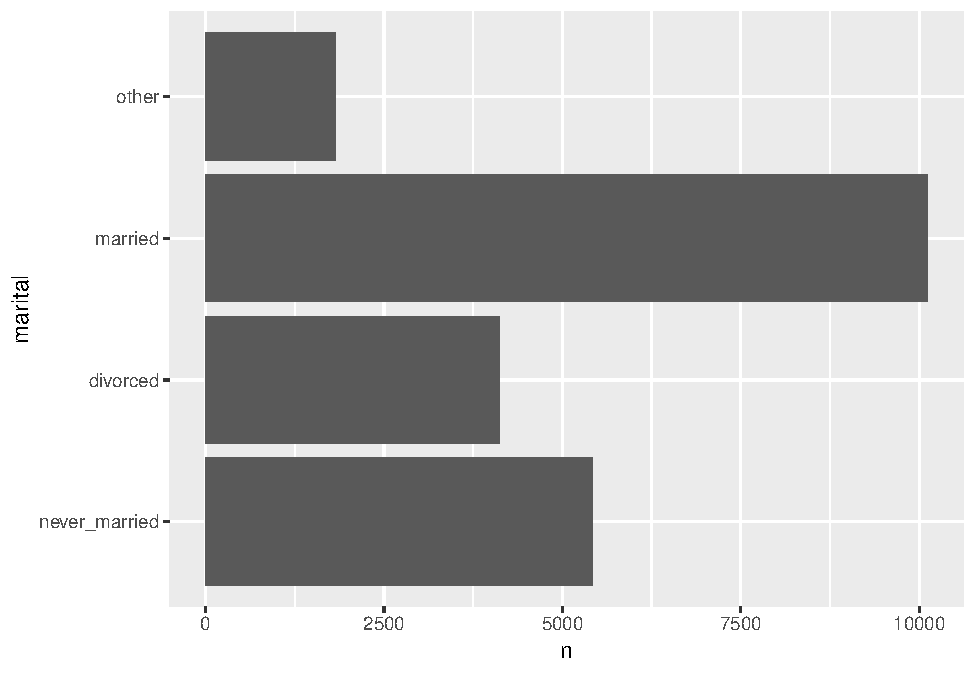
\includegraphics{modern_R_files/figure-latex/unnamed-chunk-273-1.pdf}

It would be much better if the categories were ordered by frequency.
This is easy to do with \texttt{fct\_reorder()}:

\begin{Shaded}
\begin{Highlighting}[]
\NormalTok{gss_cat }\OperatorTok
\StringTok{    }\KeywordTok{tabyl}\NormalTok{(marital) }\OperatorTok
\StringTok{    }\KeywordTok{mutate}\NormalTok{(}\DataTypeTok{marital =} \KeywordTok{fct_reorder}\NormalTok{(marital, n, }\DataTypeTok{.desc =} \OtherTok{FALSE}\NormalTok{)) }\OperatorTok
\StringTok{    }\KeywordTok{ggplot}\NormalTok{() }\OperatorTok{+}
\StringTok{    }\KeywordTok{geom_col}\NormalTok{(}\KeywordTok{aes}\NormalTok{(}\DataTypeTok{y =}\NormalTok{ n, }\DataTypeTok{x =}\NormalTok{ marital)) }\OperatorTok{+}
\StringTok{    }\KeywordTok{coord_flip}\NormalTok{()}
\end{Highlighting}
\end{Shaded}

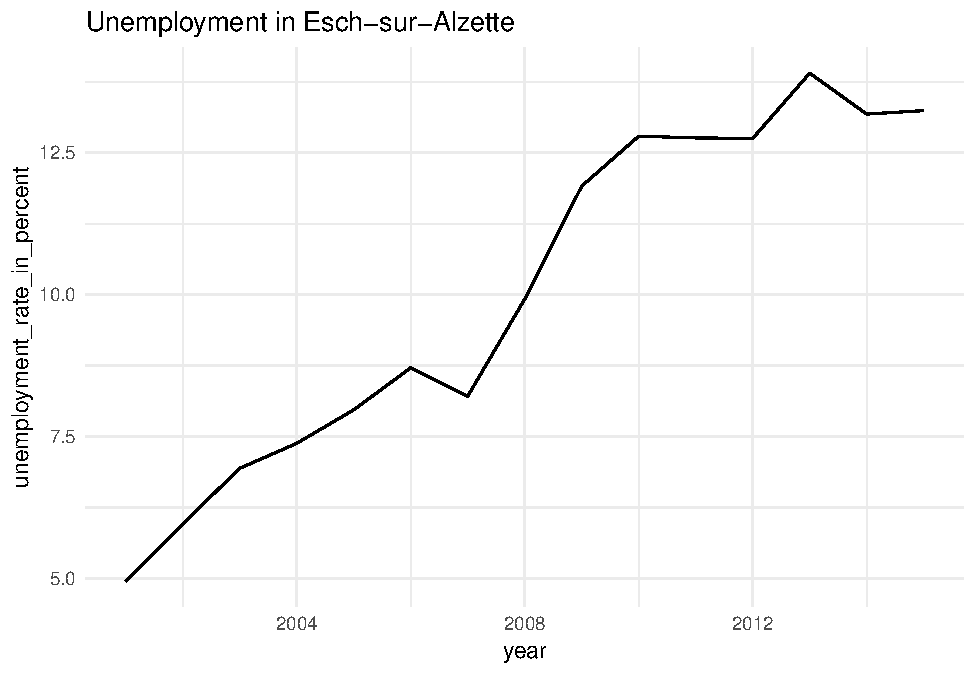
\includegraphics{modern_R_files/figure-latex/unnamed-chunk-274-1.pdf}

Much better! In Chapter 6, we are going to learn about
\texttt{\{ggplot2\}}.

\texttt{\{forcats\}} contains other very useful functions, so I urge you
to go through the documentation.

\hypertarget{get-your-dates-right-with-lubridate}{%
\subsubsection{\texorpdfstring{Get your dates right with
\texttt{\{lubridate\}}}{Get your dates right with \{lubridate\}}}\label{get-your-dates-right-with-lubridate}}

\texttt{\{lubridate\}} is yet another tidyverse package, that makes
dealing with dates or durations (and intervals) as painless as possible.
I do not use every function contained in the package daily, and as such
will only focus on some of the functions. However, if you have to deal
with dates often, you might want to explore the package thouroughly.

\hypertarget{defining-dates-the-tidy-way}{%
\paragraph{Defining dates, the tidy
way}\label{defining-dates-the-tidy-way}}

Let's load new dataset, called \emph{independence} from the datasets
folder:

\begin{Shaded}
\begin{Highlighting}[]
\NormalTok{independence <-}\StringTok{ }\KeywordTok{readRDS}\NormalTok{(}\StringTok{"datasets/independence.rds"}\NormalTok{)}
\end{Highlighting}
\end{Shaded}

This dataset was scraped from the following Wikipedia
\href{https://en.wikipedia.org/wiki/Decolonisation_of_Africa\#Timeline}{page}.
It shows when African countries gained independence from which colonial
powers. In Chapter 11, I will show you how to scrape Wikipedia pages
using R. For now, let's take a look at the contents of the dataset:

\begin{Shaded}
\begin{Highlighting}[]
\NormalTok{independence}
\end{Highlighting}
\end{Shaded}

\begin{verbatim}
## # A tibble: 54 x 6
##    country colonial_name colonial_power independence_da~ first_head_of_s~
##    <chr>   <chr>         <chr>          <chr>            <chr>           
##  1 Liberia Liberia       United States  26 July 1847     Joseph Jenkins ~
##  2 South ~ Cape Colony ~ United Kingdom 31 May 1910      Louis Botha     
##  3 Egypt   Sultanate of~ United Kingdom 28 February 1922 Fuad I          
##  4 Eritrea Italian Erit~ Italy          10 February 1947 Haile Selassie  
##  5 Libya   British Mili~ United Kingdo~ 24 December 1951 Idris           
##  6 Sudan   Anglo-Egypti~ United Kingdo~ 1 January 1956   Ismail al-Azhari
##  7 Tunisia French Prote~ France         20 March 1956    Muhammad VIII a~
##  8 Morocco French Prote~ France Spain   2 March 19567 A~ Mohammed V      
##  9 Ghana   Gold Coast    United Kingdom 6 March 1957     Kwame Nkrumah   
## 10 Guinea  French West ~ France         2 October 1958   Ahmed Sékou Tou~
## # ... with 44 more rows, and 1 more variable:
## #   independence_won_through <chr>
\end{verbatim}

as you can see, the date of independence is in a format that might make
it difficult to answer questions such as \emph{Which African countries
gained independence before 1960 ?} for two reasons. First of all, the
date uses the name of the month instead of the number of the month, and
second of all the type of the independence day column is
\emph{character} and not ``date''. So our first task is to correctly
define the column as being of type date, while making sure that R
understands that \emph{January} is supposed to be ``01'', and so on.
There are several helpful functions included in \texttt{\{lubridate\}}
to convert columns to dates. For instance if the column you want to
convert is of the form ``2012-11-21'', then you would use the function
\texttt{ymd()}, for ``year-month-day''. If, however the column is
``2012-21-11'', then you would use \texttt{ydm()}. There's a few of
these helper functions, and they can handle a lot of different formats
for dates. In our case, having the name of the month instead of the
number might seem quite problematic, but it turns out that this is a
case that \texttt{\{lubridate\}} handles painfully:

\begin{Shaded}
\begin{Highlighting}[]
\KeywordTok{library}\NormalTok{(lubridate)}
\end{Highlighting}
\end{Shaded}

\begin{verbatim}
## 
## Attaching package: 'lubridate'
\end{verbatim}

\begin{verbatim}
## The following object is masked from 'package:base':
## 
##     date
\end{verbatim}

\begin{Shaded}
\begin{Highlighting}[]
\NormalTok{independence <-}\StringTok{ }\NormalTok{independence }\OperatorTok
\StringTok{  }\KeywordTok{mutate}\NormalTok{(}\DataTypeTok{independence_date =} \KeywordTok{dmy}\NormalTok{(independence_date))}
\end{Highlighting}
\end{Shaded}

\begin{verbatim}
## Warning: 5 failed to parse.
\end{verbatim}

Some dates failed to parse, for instance for Morocco. This is because
these countries have several independence dates; this means that the
string to convert looks like:

\begin{verbatim}
"2 March 1956
7 April 1956
10 April 1958
4 January 1969"
\end{verbatim}

which obviously cannot be converted by \texttt{\{lubridate\}} without
further manipulation. I ignore these cases for simplicity's sake.

Let's take a look at the data now:

\begin{Shaded}
\begin{Highlighting}[]
\NormalTok{independence}
\end{Highlighting}
\end{Shaded}

\begin{verbatim}
## # A tibble: 54 x 6
##    country colonial_name colonial_power independence_da~ first_head_of_s~
##    <chr>   <chr>         <chr>          <date>           <chr>           
##  1 Liberia Liberia       United States  1847-07-26       Joseph Jenkins ~
##  2 South ~ Cape Colony ~ United Kingdom 1910-05-31       Louis Botha     
##  3 Egypt   Sultanate of~ United Kingdom 1922-02-28       Fuad I          
##  4 Eritrea Italian Erit~ Italy          1947-02-10       Haile Selassie  
##  5 Libya   British Mili~ United Kingdo~ 1951-12-24       Idris           
##  6 Sudan   Anglo-Egypti~ United Kingdo~ 1956-01-01       Ismail al-Azhari
##  7 Tunisia French Prote~ France         1956-03-20       Muhammad VIII a~
##  8 Morocco French Prote~ France Spain   NA               Mohammed V      
##  9 Ghana   Gold Coast    United Kingdom 1957-03-06       Kwame Nkrumah   
## 10 Guinea  French West ~ France         1958-10-02       Ahmed Sékou Tou~
## # ... with 44 more rows, and 1 more variable:
## #   independence_won_through <chr>
\end{verbatim}

As you can see, we now have a date column in the right format. We can
now answer questions such as \emph{Which countries gained independence
before 1960?} quite easily, by using the functions \texttt{year()},
\texttt{month()} and \texttt{day()}. Let's see which countries gained
independence before 1960:

\begin{Shaded}
\begin{Highlighting}[]
\NormalTok{independence }\OperatorTok
\StringTok{  }\KeywordTok{filter}\NormalTok{(}\KeywordTok{year}\NormalTok{(independence_date) }\OperatorTok{<=}\StringTok{ }\DecValTok{1960}\NormalTok{) }\OperatorTok
\StringTok{  }\KeywordTok{pull}\NormalTok{(country)}
\end{Highlighting}
\end{Shaded}

\begin{verbatim}
##  [1] "Liberia"                          "South Africa"                    
##  [3] "Egypt"                            "Eritrea"                         
##  [5] "Libya"                            "Sudan"                           
##  [7] "Tunisia"                          "Ghana"                           
##  [9] "Guinea"                           "Cameroon"                        
## [11] "Togo"                             "Mali"                            
## [13] "Madagascar"                       "Democratic Republic of the Congo"
## [15] "Benin"                            "Niger"                           
## [17] "Burkina Faso"                     "Ivory Coast"                     
## [19] "Chad"                             "Central African Republic"        
## [21] "Republic of the Congo"            "Gabon"                           
## [23] "Mauritania"
\end{verbatim}

You guessed it, \texttt{year()} extracts the year of the date column and
converts it as a \emph{numeric} so that we can work on it. This is the
same for \texttt{month()} or \texttt{day()}. Let's try to see if
countries gained their independence on Christmas Eve:

\begin{Shaded}
\begin{Highlighting}[]
\NormalTok{independence }\OperatorTok
\StringTok{  }\KeywordTok{filter}\NormalTok{(}\KeywordTok{month}\NormalTok{(independence_date) }\OperatorTok{==}\StringTok{ }\DecValTok{12}\NormalTok{,}
         \KeywordTok{day}\NormalTok{(independence_date) }\OperatorTok{==}\StringTok{ }\DecValTok{24}\NormalTok{) }\OperatorTok
\StringTok{  }\KeywordTok{pull}\NormalTok{(country)}
\end{Highlighting}
\end{Shaded}

\begin{verbatim}
## [1] "Libya"
\end{verbatim}

Seems like Libya was the only one! You can also operate on dates. For
instance, let's compute the difference between two dates, using the
\texttt{interval()} column:

\begin{Shaded}
\begin{Highlighting}[]
\NormalTok{independence }\OperatorTok
\StringTok{  }\KeywordTok{mutate}\NormalTok{(}\DataTypeTok{today =}\NormalTok{ lubridate}\OperatorTok{::}\KeywordTok{today}\NormalTok{()) }\OperatorTok
\StringTok{  }\KeywordTok{mutate}\NormalTok{(}\DataTypeTok{independent_since =} \KeywordTok{interval}\NormalTok{(independence_date, today)) }\OperatorTok
\StringTok{  }\KeywordTok{select}\NormalTok{(country, independent_since)}
\end{Highlighting}
\end{Shaded}

\begin{verbatim}
## # A tibble: 54 x 2
##    country      independent_since             
##    <chr>        <S4: Interval>                
##  1 Liberia      1847-07-26 UTC--2018-12-15 UTC
##  2 South Africa 1910-05-31 UTC--2018-12-15 UTC
##  3 Egypt        1922-02-28 UTC--2018-12-15 UTC
##  4 Eritrea      1947-02-10 UTC--2018-12-15 UTC
##  5 Libya        1951-12-24 UTC--2018-12-15 UTC
##  6 Sudan        1956-01-01 UTC--2018-12-15 UTC
##  7 Tunisia      1956-03-20 UTC--2018-12-15 UTC
##  8 Morocco      NA--NA                        
##  9 Ghana        1957-03-06 UTC--2018-12-15 UTC
## 10 Guinea       1958-10-02 UTC--2018-12-15 UTC
## # ... with 44 more rows
\end{verbatim}

The \texttt{independent\_since} column now contains an \emph{interval}
object that we can convert to years:

\begin{Shaded}
\begin{Highlighting}[]
\NormalTok{independence }\OperatorTok
\StringTok{  }\KeywordTok{mutate}\NormalTok{(}\DataTypeTok{today =}\NormalTok{ lubridate}\OperatorTok{::}\KeywordTok{today}\NormalTok{()) }\OperatorTok
\StringTok{  }\KeywordTok{mutate}\NormalTok{(}\DataTypeTok{independent_since =} \KeywordTok{interval}\NormalTok{(independence_date, today)) }\OperatorTok
\StringTok{  }\KeywordTok{select}\NormalTok{(country, independent_since) }\OperatorTok
\StringTok{  }\KeywordTok{mutate}\NormalTok{(}\DataTypeTok{years_independent =} \KeywordTok{as.numeric}\NormalTok{(independent_since, }\StringTok{"years"}\NormalTok{))}
\end{Highlighting}
\end{Shaded}

\begin{verbatim}
## # A tibble: 54 x 3
##    country      independent_since              years_independent
##    <chr>        <S4: Interval>                             <dbl>
##  1 Liberia      1847-07-26 UTC--2018-12-15 UTC             171. 
##  2 South Africa 1910-05-31 UTC--2018-12-15 UTC             109. 
##  3 Egypt        1922-02-28 UTC--2018-12-15 UTC              96.8
##  4 Eritrea      1947-02-10 UTC--2018-12-15 UTC              71.8
##  5 Libya        1951-12-24 UTC--2018-12-15 UTC              67.0
##  6 Sudan        1956-01-01 UTC--2018-12-15 UTC              63.0
##  7 Tunisia      1956-03-20 UTC--2018-12-15 UTC              62.7
##  8 Morocco      NA--NA                                      NA  
##  9 Ghana        1957-03-06 UTC--2018-12-15 UTC              61.8
## 10 Guinea       1958-10-02 UTC--2018-12-15 UTC              60.2
## # ... with 44 more rows
\end{verbatim}

We can now see for how long the last country to gain independence has
been independent. Because the data is not tidy (in some cases, an
African country was colonized by two powers, see Libya), I will only
focus on 4 European colonial powers: Belgium, France, Portugal and the
United Kingdom:

\begin{Shaded}
\begin{Highlighting}[]
\NormalTok{independence }\OperatorTok
\StringTok{  }\KeywordTok{filter}\NormalTok{(colonial_power }\OperatorTok\StringTok{ }\KeywordTok{c}\NormalTok{(}\StringTok{"Belgium"}\NormalTok{, }\StringTok{"France"}\NormalTok{, }\StringTok{"Portugal"}\NormalTok{, }\StringTok{"United Kingdom"}\NormalTok{)) }\OperatorTok
\StringTok{  }\KeywordTok{mutate}\NormalTok{(}\DataTypeTok{today =}\NormalTok{ lubridate}\OperatorTok{::}\KeywordTok{today}\NormalTok{()) }\OperatorTok
\StringTok{  }\KeywordTok{mutate}\NormalTok{(}\DataTypeTok{independent_since =} \KeywordTok{interval}\NormalTok{(independence_date, today)) }\OperatorTok
\StringTok{  }\KeywordTok{mutate}\NormalTok{(}\DataTypeTok{years_independent =} \KeywordTok{as.numeric}\NormalTok{(independent_since, }\StringTok{"years"}\NormalTok{)) }\OperatorTok
\StringTok{  }\KeywordTok{group_by}\NormalTok{(colonial_power) }\OperatorTok
\StringTok{  }\KeywordTok{summarise}\NormalTok{(}\DataTypeTok{last_colony_independent_for =} \KeywordTok{min}\NormalTok{(years_independent, }\DataTypeTok{na.rm =} \OtherTok{TRUE}\NormalTok{))}
\end{Highlighting}
\end{Shaded}

\begin{verbatim}
## # A tibble: 4 x 2
##   colonial_power last_colony_independent_for
##   <chr>                                <dbl>
## 1 Belgium                               56.5
## 2 France                                41.5
## 3 Portugal                              43.1
## 4 United Kingdom                        42.5
\end{verbatim}

\texttt{\{lubridate\}} contains many more functions. If you often work
with dates, duration or interval data, \texttt{\{lubridate\}} is a
package that you have to master.

\hypertarget{manipulate-strings-with-stringr}{%
\subsubsection{\texorpdfstring{Manipulate strings with
\texttt{\{stringr\}}}{Manipulate strings with \{stringr\}}}\label{manipulate-strings-with-stringr}}

\texttt{\{stringr\}} contains functions to manipulate strings. In
Chapter 11, I will teach you about regular expressions, but the
functions contained in \texttt{\{stringr\}} allow you to already do a
lot of work on strings, without needing to be a regular expression
expert.

I will discuss the most common string operations: search and replace (or
remove), detect, locate or match, and trim a string.

\hypertarget{list-columns}{%
\subsection{List-columns}\label{list-columns}}

To learn about list-columns, let's first focus on a single character of
the \texttt{starwars} dataset:

\begin{Shaded}
\begin{Highlighting}[]
\KeywordTok{data}\NormalTok{(starwars)}
\end{Highlighting}
\end{Shaded}

\begin{Shaded}
\begin{Highlighting}[]
\NormalTok{starwars }\OperatorTok
\StringTok{  }\KeywordTok{filter}\NormalTok{(name }\OperatorTok{==}\StringTok{ "Luke Skywalker"}\NormalTok{) }\OperatorTok
\StringTok{  }\KeywordTok{glimpse}\NormalTok{()}
\end{Highlighting}
\end{Shaded}

\begin{verbatim}
## Observations: 1
## Variables: 13
## $ name       <chr> "Luke Skywalker"
## $ height     <int> 172
## $ mass       <dbl> 77
## $ hair_color <chr> "blond"
## $ skin_color <chr> "fair"
## $ eye_color  <chr> "blue"
## $ birth_year <dbl> 19
## $ gender     <chr> "male"
## $ homeworld  <chr> "Tatooine"
## $ species    <chr> "Human"
## $ films      <list> [<"Revenge of the Sith", "Return of the Jedi", "Th...
## $ vehicles   <list> [<"Snowspeeder", "Imperial Speeder Bike">]
## $ starships  <list> [<"X-wing", "Imperial shuttle">]
\end{verbatim}

We see that the columns \texttt{films}, \texttt{vehicles} and
\texttt{starships} are all lists, and in the case of \texttt{films}, it
lists all the films where Luke Skywalker has appeared. What if you want
to take a closer look at this list?

\begin{Shaded}
\begin{Highlighting}[]
\NormalTok{starwars }\OperatorTok
\StringTok{  }\KeywordTok{filter}\NormalTok{(name }\OperatorTok{==}\StringTok{ "Luke Skywalker"}\NormalTok{) }\OperatorTok
\StringTok{  }\KeywordTok{pull}\NormalTok{(films)}
\end{Highlighting}
\end{Shaded}

\begin{verbatim}
## [[1]]
## [1] "Revenge of the Sith"     "Return of the Jedi"     
## [3] "The Empire Strikes Back" "A New Hope"             
## [5] "The Force Awakens"
\end{verbatim}

\texttt{pull()} is a \texttt{dplyr} function that extract (pulls) the
column you're interested in. It is quite useful when you want to inspect
a column.

Suppose we want to create a categorical variable which counts the number
of movies in which the characters have appeared. For this we need to
compute the length of the list, or count the number of elements this
list has. Let's try with \texttt{length()} a base R function:

\begin{Shaded}
\begin{Highlighting}[]
\NormalTok{starwars }\OperatorTok
\StringTok{  }\KeywordTok{filter}\NormalTok{(name }\OperatorTok{==}\StringTok{ "Luke Skywalker"}\NormalTok{) }\OperatorTok
\StringTok{  }\KeywordTok{pull}\NormalTok{(films) }\OperatorTok
\StringTok{  }\KeywordTok{length}\NormalTok{()}
\end{Highlighting}
\end{Shaded}

\begin{verbatim}
## [1] 1
\end{verbatim}

This might be surprising at first, because we know that Luke Skywalker
has appeared in more than 1 movie\ldots{} the problem here is that for
each individual, \texttt{films} is a list, whose single element is a
vector of characters. This means that \texttt{length(films)} computes
the length of the list, which is one, and not the length of the vector
contained in the list! How can we get the length of the vector of
characters contained in the list and for each character? For this we
need to use \texttt{dplyr::rowwise()} and remove the \texttt{filter()}
function and use \texttt{mutate()} to add this column to the dataset:

\begin{Shaded}
\begin{Highlighting}[]
\NormalTok{starwars <-}\StringTok{ }\NormalTok{starwars }\OperatorTok
\StringTok{  }\KeywordTok{rowwise}\NormalTok{() }\OperatorTok
\StringTok{  }\KeywordTok{mutate}\NormalTok{(}\DataTypeTok{n_films =} \KeywordTok{length}\NormalTok{(films))}
\end{Highlighting}
\end{Shaded}

\texttt{dplyr::rowwise()} is useful when working with list-columns:
columns that have lists as elements.

Let's take a look at the characters and the number of films they have
appeared in:

\begin{Shaded}
\begin{Highlighting}[]
\NormalTok{starwars }\OperatorTok
\StringTok{  }\KeywordTok{select}\NormalTok{(name, n_films)}
\end{Highlighting}
\end{Shaded}

\begin{verbatim}
## Source: local data frame [87 x 2]
## Groups: <by row>
## 
## # A tibble: 87 x 2
##    name               n_films
##    <chr>                <int>
##  1 Luke Skywalker           5
##  2 C-3PO                    6
##  3 R2-D2                    7
##  4 Darth Vader              4
##  5 Leia Organa              5
##  6 Owen Lars                3
##  7 Beru Whitesun lars       3
##  8 R5-D4                    1
##  9 Biggs Darklighter        1
## 10 Obi-Wan Kenobi           6
## # ... with 77 more rows
\end{verbatim}

Now we can create a factor variable that groups characters by asking
whether they appeared only in 1 movie, or more:

\begin{Shaded}
\begin{Highlighting}[]
\NormalTok{starwars <-}\StringTok{ }\NormalTok{starwars }\OperatorTok
\StringTok{  }\KeywordTok{mutate}\NormalTok{(}\DataTypeTok{more_1 =} \KeywordTok{case_when}\NormalTok{(n_films }\OperatorTok{==}\StringTok{ }\DecValTok{1} \OperatorTok{~}\StringTok{ "Exactly one movie"}\NormalTok{,}
\NormalTok{                            n_films }\OperatorTok{!=}\StringTok{ }\DecValTok{1} \OperatorTok{~}\StringTok{ "More than 1 movie"}\NormalTok{))}
\end{Highlighting}
\end{Shaded}

\texttt{case\_when()} is a \texttt{dplyr} function that works similarly
to the standard \texttt{if..else..} construct of many programming
languages (R also has this, we are going to learn about it in later
chapters).

You can also create list columns with your own datasets, by using
\texttt{tidyr::nest()}. Remember the fake \texttt{survey\_data} I
created to illustrate \texttt{spread()} and \texttt{gather()}? Let's go
back to that dataset again:

\begin{Shaded}
\begin{Highlighting}[]
\KeywordTok{print}\NormalTok{(survey_data)}
\end{Highlighting}
\end{Shaded}

\begin{verbatim}
## # A tibble: 12 x 3
##       id variable value
##    <dbl> <chr>    <dbl>
##  1     1 var1       1  
##  2     1 var2       0.2
##  3    NA var3       0.3
##  4     2 var1       1.4
##  5     2 var2       1.9
##  6     2 var3       4.1
##  7     3 var1       0.1
##  8     3 var2       2.8
##  9     3 var3       8.9
## 10     4 var1       1.7
## 11    NA var2       1.9
## 12     4 var3       7.6
\end{verbatim}

\begin{Shaded}
\begin{Highlighting}[]
\NormalTok{nested_data =}\StringTok{ }\NormalTok{survey_data }\OperatorTok
\StringTok{  }\KeywordTok{nest}\NormalTok{(variable, value)}

\KeywordTok{print}\NormalTok{(nested_data)}
\end{Highlighting}
\end{Shaded}

\begin{verbatim}
## # A tibble: 5 x 2
##      id data            
##   <dbl> <list>          
## 1     1 <tibble [2 x 2]>
## 2    NA <tibble [2 x 2]>
## 3     2 <tibble [3 x 2]>
## 4     3 <tibble [3 x 2]>
## 5     4 <tibble [2 x 2]>
\end{verbatim}

This creates a new tibble, with columns \texttt{id} and \texttt{data}.
\texttt{data} is a list-column that contains tibbles; each tibble is the
\texttt{variable} and \texttt{value} for each individual:

\begin{Shaded}
\begin{Highlighting}[]
\NormalTok{nested_data }\OperatorTok
\StringTok{  }\KeywordTok{filter}\NormalTok{(id }\OperatorTok{==}\StringTok{ "1"}\NormalTok{) }\OperatorTok
\StringTok{  }\KeywordTok{pull}\NormalTok{(data)}
\end{Highlighting}
\end{Shaded}

\begin{verbatim}
## [[1]]
## # A tibble: 2 x 2
##   variable value
##   <chr>    <dbl>
## 1 var1       1  
## 2 var2       0.2
\end{verbatim}

As you can see, for individual 1, the column data contains a 2x2 tibble
with columns \texttt{variable} and \texttt{value}. You might be
wondering why this is useful, because this seems to introduce an
unnecessary layer of complexity. The usefulness of list-columns will
become apparent in the next chapters, where we are going to learn how to
repeat actions over, say, individuals.

\hypertarget{exercises-2}{%
\subsection{Exercises}\label{exercises-2}}

\hypertarget{exercise-1-2}{%
\subsubsection*{Exercise 1}\label{exercise-1-2}}
\addcontentsline{toc}{subsubsection}{Exercise 1}

Load the \texttt{LaborSupply} dataset from the \texttt{Ecdat} package
and answer the following questions:

\begin{itemize}
\tightlist
\item
  Compute the average annual hours worked by year (plus standard
  deviation)
\item
  What age group worked the most hours in the year 1982?
\item
  Create a variable, \texttt{n\_years} that equals the number of years
  an individual stays in the panel. Is the panel balanced?
\item
  Which are the individuals that do not have any kids during the whole
  period? Create a variable, \texttt{no\_kids}, that flags these
  individuals (1 = no kids, 0 = kids)
\item
  Using the \texttt{no\_kids} variable from before compute the average
  wage, standard deviation and number of observations in each group for
  the year 1980 (no kids group vs kids group).
\item
  Create the lagged logarithm of hours worked and wages. Remember that
  this is a panel.
\end{itemize}

\hypertarget{exercise-2-1}{%
\subsubsection*{Exercise 2}\label{exercise-2-1}}
\addcontentsline{toc}{subsubsection}{Exercise 2}

\begin{itemize}
\tightlist
\item
  What does the following code do? Copy and paste it in an R interpreter
  to find out!
\end{itemize}

\begin{Shaded}
\begin{Highlighting}[]
\NormalTok{LaborSupply }\OperatorTok
\StringTok{  }\KeywordTok{group_by}\NormalTok{(id) }\OperatorTok
\StringTok{  }\KeywordTok{mutate_at}\NormalTok{(}\KeywordTok{vars}\NormalTok{(}\KeywordTok{starts_with}\NormalTok{(}\StringTok{"l"}\NormalTok{)), }\KeywordTok{funs}\NormalTok{(lag, lead))}
\end{Highlighting}
\end{Shaded}

\texttt{mutate\_at()} is a scoped version of \texttt{mutate()} which
allows you to specify a number of columns and functions in one go. This
also exists for \texttt{summarise()}.

\begin{itemize}
\tightlist
\item
  Using \texttt{summarise\_at()}, compute the mean, standard deviation
  and number of individuals of \texttt{lnhr} and \texttt{lnwg} for each
  individual.
\end{itemize}

\hypertarget{exercise-3-1}{%
\subsubsection*{Exercise 3}\label{exercise-3-1}}
\addcontentsline{toc}{subsubsection}{Exercise 3}

\begin{itemize}
\item
  In the dataset folder you downloaded at the beginning of the chapter,
  there is a folder called ``unemployment''. I used the data in the
  section about working with lists of datasets. Using
  \texttt{rio::import\_list()}, read the 4 datasets into R.
\item
  Using \texttt{map()}, map the \texttt{janitor::clean\_names()}
  function to each dataset (just like in the example in the section on
  working with lists of datasets). Then, still with \texttt{map()} and
  \texttt{mutate()} convert all commune names in the \texttt{commune}
  column with the function \texttt{tolower()}, in a new column called
  \texttt{lcommune}. This is not an easy exercise; so here are some
  hints:

  \begin{itemize}
  \tightlist
  \item
    Remember that \texttt{all\_datasets} is a list of datasets. Which
    function do you use when you want to map a function to each element
    of a list?
  \item
    Each element of \texttt{all\_datasets} are \texttt{data.frame}
    objects. Which function do you use to add a column to a
    \texttt{data.frame}?
  \item
    What symbol can you use to access a column of a \texttt{data.frame}?
  \end{itemize}
\end{itemize}

\hypertarget{graphs}{%
\section{Graphs}\label{graphs}}

By default, it is possible to make a lot of graphs with R without the
need of any external packages. However, in this chapter, we are going to
learn how to make graphs using \texttt{ggplot2} which is a very powerful
package that produces amazing graphs. There is an entry cost to
\texttt{ggplot2} as it works in a very different way than what you would
expect, especially if you know how to make plots with the basic R
functions already. But the resulting graphs are well worth the effort
and once you'll know more about \texttt{ggplot2} you'll see that in a
lot of situations it is actually faster and easier. Even if you are not
interested in drawing plots, I advise you continue reading, as we will
dig deeper into functional programming territory and learn how to graph
an arbitrary large amount of plots with a few lines of code.

\hypertarget{resources}{%
\subsection{Resources}\label{resources}}

Before showing some examples and the general functionality of
\texttt{ggplot2}, I list here some online resources that I keep coming
back to:

\begin{itemize}
\item
  \href{http://socviz.co/}{Data Visualization for Social Science}
\item
  \href{http://www.cookbook-r.com/Graphs/}{R Graphics Cookbook}
\item
  \href{http://www.r-graph-gallery.com/portfolio/ggplot2-package/}{R
  graph gallery}
\item
  \href{http://motioninsocial.com/tufte/}{Tufte in R}
\item
  \href{http://www.ggplot2-exts.org/gallery/}{ggplot2 extensions}
\item
  \href{https://cran.r-project.org/web/packages/ggthemes/vignettes/ggthemes.html}{ggthemes
  Vignette}
\item
  \href{https://www.rstudio.com/wp-content/uploads/2015/03/ggplot2-cheatsheet.pdf}{ggplot2
  cheatsheet}
\end{itemize}

I have a cookbook approach to using \texttt{ggplot2}; I try to find an
example online that looks similar to what I have in mind, copy and paste
the code and then adapt it to my case. The above resources are the ones
I consult the most in these situations (I also go back to past code I've
written, of course). Don't hesitate to skim these resources for
inspiration and to learn more about some extensions to \texttt{ggplot2}.
In the next subsections I am going to show you how to draw the most
common plots, as well as show you how to customize your plots with
\texttt{ggthemes}.

\hypertarget{examples}{%
\subsection{Examples}\label{examples}}

\hypertarget{barplots}{%
\subsubsection{Barplots}\label{barplots}}

To follow the examples below, load the following libraries:

\begin{Shaded}
\begin{Highlighting}[]
\KeywordTok{library}\NormalTok{(ggplot2)}
\KeywordTok{library}\NormalTok{(ggthemes)}
\end{Highlighting}
\end{Shaded}

\texttt{ggplot2} is an implementation of the \emph{Grammar of Graphics}
by \citet{wilkinson2006}, but you don't need to read the books to start
using it. If we go back to the Star Wars data (contained in
\texttt{dplyr}), and wish to draw a barplot of the gender, the following
lines are enough:

\begin{Shaded}
\begin{Highlighting}[]
\KeywordTok{ggplot}\NormalTok{(starwars, }\KeywordTok{aes}\NormalTok{(gender)) }\OperatorTok{+}
\StringTok{  }\KeywordTok{geom_bar}\NormalTok{()}
\end{Highlighting}
\end{Shaded}

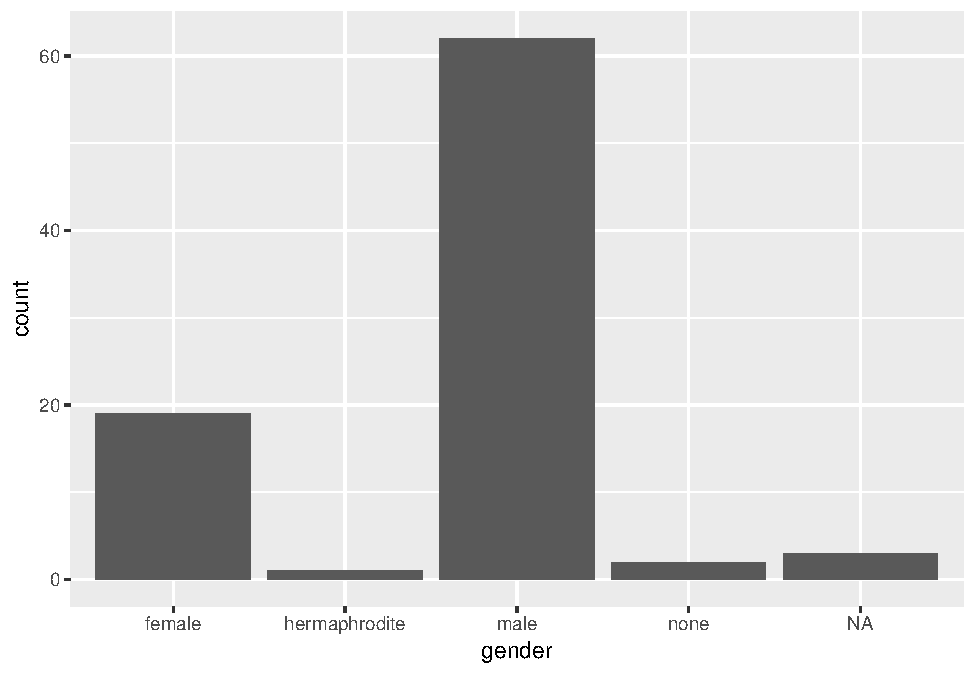
\includegraphics{modern_R_files/figure-latex/unnamed-chunk-300-1.pdf}

The first argument of the function is the data (called \texttt{starwars}
in this example), and then the function \texttt{aes()}. This function is
where you list the variables you want to map, and to quote the help file
of \texttt{aes()}, \emph{describes how the variables are mapped to
visual properties (aesthetics) of geoms}. You can get different kind of
plots by using different \texttt{geom\_} functions.

You can also change the coordinate system in your barplot:

\begin{Shaded}
\begin{Highlighting}[]
\KeywordTok{ggplot}\NormalTok{(starwars, }\KeywordTok{aes}\NormalTok{(gender)) }\OperatorTok{+}
\StringTok{  }\KeywordTok{geom_bar}\NormalTok{() }\OperatorTok{+}
\StringTok{  }\KeywordTok{coord_flip}\NormalTok{()}
\end{Highlighting}
\end{Shaded}

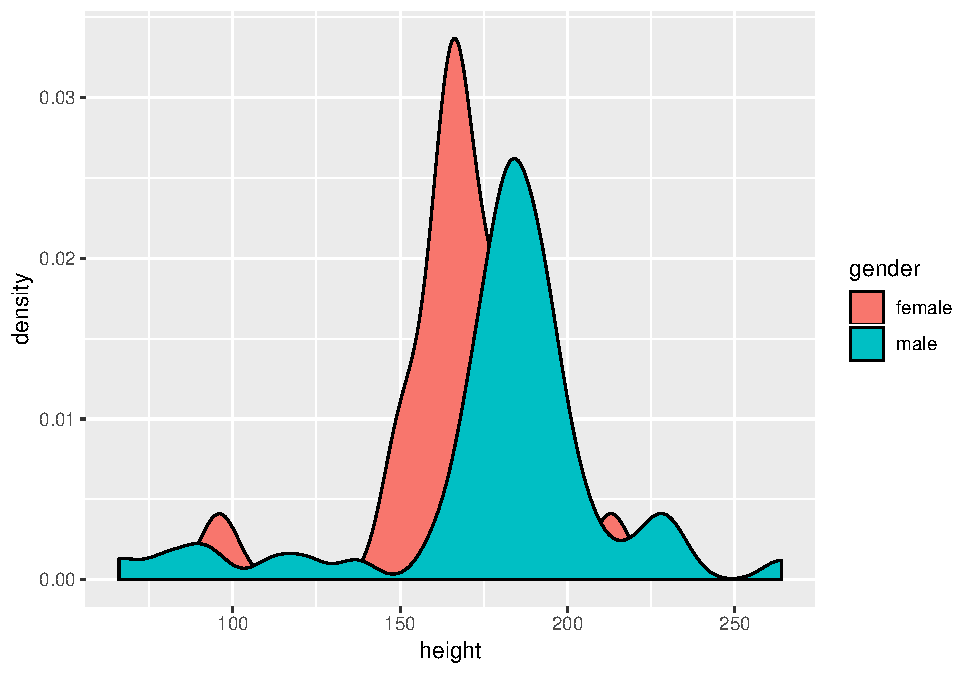
\includegraphics{modern_R_files/figure-latex/unnamed-chunk-301-1.pdf}

\hypertarget{density}{%
\subsubsection{Density}\label{density}}

\texttt{geom\_density()} is the \emph{geom} that allows you to get
density plots:

\begin{Shaded}
\begin{Highlighting}[]
\KeywordTok{ggplot}\NormalTok{(starwars, }\KeywordTok{aes}\NormalTok{(height)) }\OperatorTok{+}
\StringTok{  }\KeywordTok{geom_density}\NormalTok{()}
\end{Highlighting}
\end{Shaded}

\begin{verbatim}
## Warning: Removed 6 rows containing non-finite values (stat_density).
\end{verbatim}

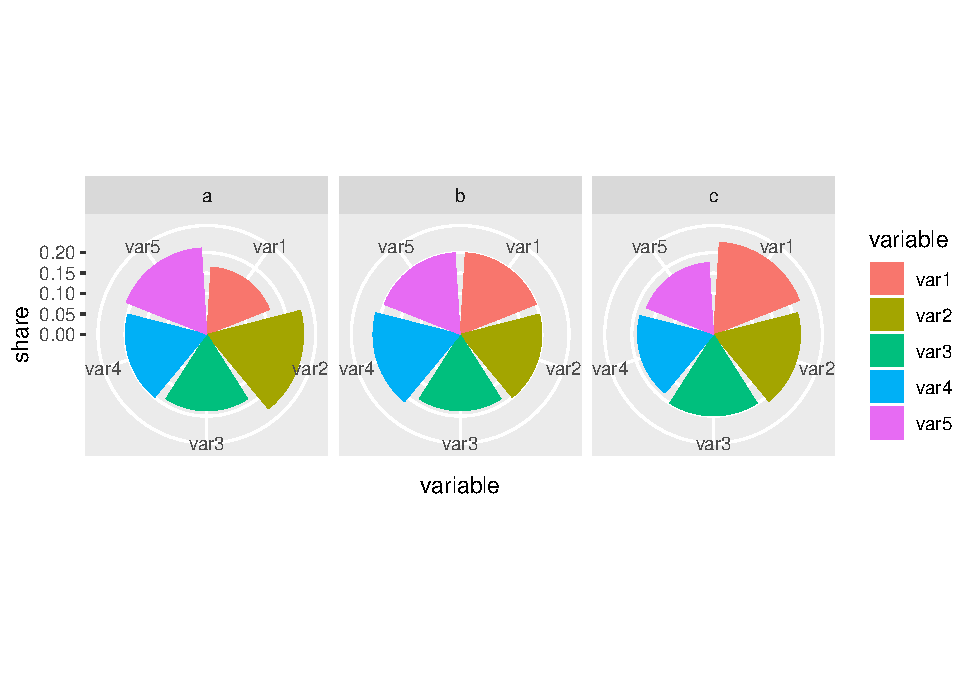
\includegraphics{modern_R_files/figure-latex/unnamed-chunk-302-1.pdf}

Let's go into more detail now; what if you would like to plot the
densities for females and males only (removing the droids from the data
first)? This can be done by first filtering the data using
\texttt{dplyr} and then separating the dataset by gender:

\begin{Shaded}
\begin{Highlighting}[]
\NormalTok{starwars }\OperatorTok
\StringTok{  }\KeywordTok{filter}\NormalTok{(gender }\OperatorTok\StringTok{ }\KeywordTok{c}\NormalTok{(}\StringTok{"female"}\NormalTok{, }\StringTok{"male"}\NormalTok{))}
\end{Highlighting}
\end{Shaded}

The above lines do the filtering; only keep gender if gender is in the
vector \texttt{"female",\ "male"}. This is much easier than having to
write \texttt{gender\ ==\ "female"\ \textbar{}\ gender\ ==\ "male"}.
Then, we pipe this dataset to \texttt{ggplot}:

\begin{Shaded}
\begin{Highlighting}[]
\NormalTok{starwars }\OperatorTok
\StringTok{  }\KeywordTok{filter}\NormalTok{(gender }\OperatorTok\StringTok{ }\KeywordTok{c}\NormalTok{(}\StringTok{"female"}\NormalTok{, }\StringTok{"male"}\NormalTok{)) }\OperatorTok
\StringTok{  }\KeywordTok{ggplot}\NormalTok{(}\KeywordTok{aes}\NormalTok{(height, }\DataTypeTok{fill =}\NormalTok{ gender)) }\OperatorTok{+}
\StringTok{  }\KeywordTok{geom_density}\NormalTok{()}
\end{Highlighting}
\end{Shaded}

\begin{verbatim}
## Warning: Removed 5 rows containing non-finite values (stat_density).
\end{verbatim}

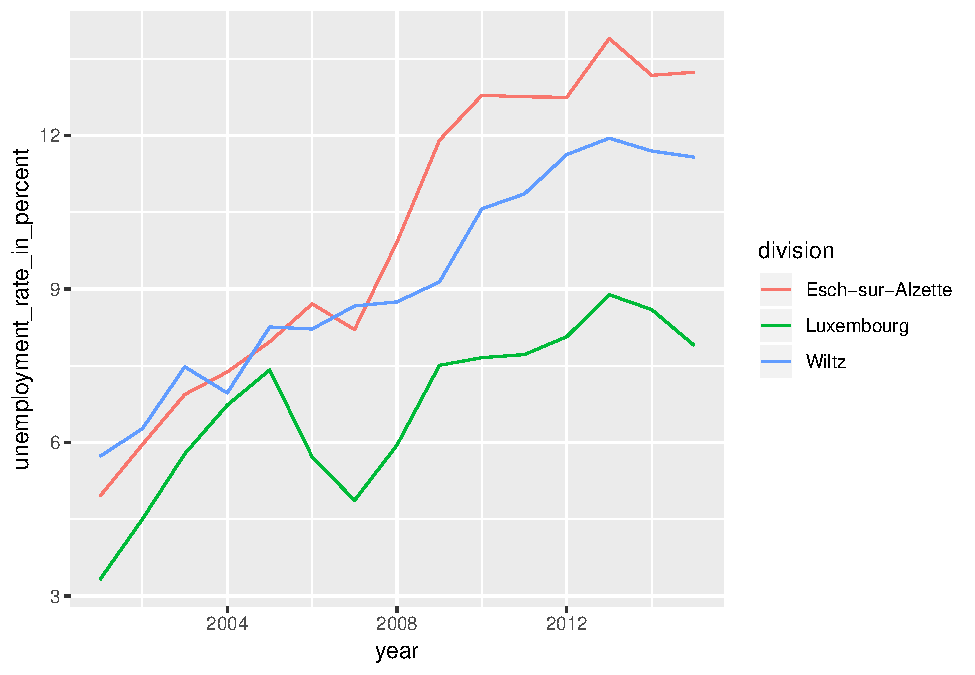
\includegraphics{modern_R_files/figure-latex/unnamed-chunk-304-1.pdf}

Let's take a closer look to the \texttt{aes()} function: I've added
\texttt{fill\ =\ gender}. This means that the there will be one density
plot for each gender in the data, and each will be coloured accordingly.
This is where \texttt{ggplot2} might be confusing; there is no need to
write explicitly (even if it is possible) that you want the
\emph{female} density to be red and the \emph{male} density to be blue.
You just map the variable \texttt{gender} to this particular aesthetic.
You conclude the plot by adding \texttt{geom\_density()} which is this
case is the plot you want. We will see later how to change the colours
of your plot.

\hypertarget{line-plots}{%
\subsubsection{Line plots}\label{line-plots}}

For the line plots, we are going to use official unemployment data (the
same as in the previous chapter, but with all the available years). Get
it from
\href{https://github.com/b-rodrigues/modern_R/tree/master/datasets/unemployment/all}{here}
(downloaded from:
\url{http://www.statistiques.public.lu/stat/TableViewer/tableView.aspx?ReportId=12950\&IF_Language=eng\&MainTheme=2\&FldrName=3\&RFPath=91}).

Let's plot the unemployment for the canton of Luxembourg only:

\begin{Shaded}
\begin{Highlighting}[]
\NormalTok{unemp_lux_data =}\StringTok{ }\KeywordTok{import}\NormalTok{(}\StringTok{"datasets/unemployment/all/unemployment_lux_all.csv"}\NormalTok{)}

\NormalTok{unemp_lux_data }\OperatorTok
\StringTok{  }\KeywordTok{filter}\NormalTok{(division }\OperatorTok{==}\StringTok{ "Luxembourg"}\NormalTok{) }\OperatorTok
\StringTok{  }\KeywordTok{ggplot}\NormalTok{(}\KeywordTok{aes}\NormalTok{(year, unemployment_rate_in_percent, }\DataTypeTok{group =} \DecValTok{1}\NormalTok{)) }\OperatorTok{+}
\StringTok{  }\KeywordTok{geom_line}\NormalTok{()}
\end{Highlighting}
\end{Shaded}

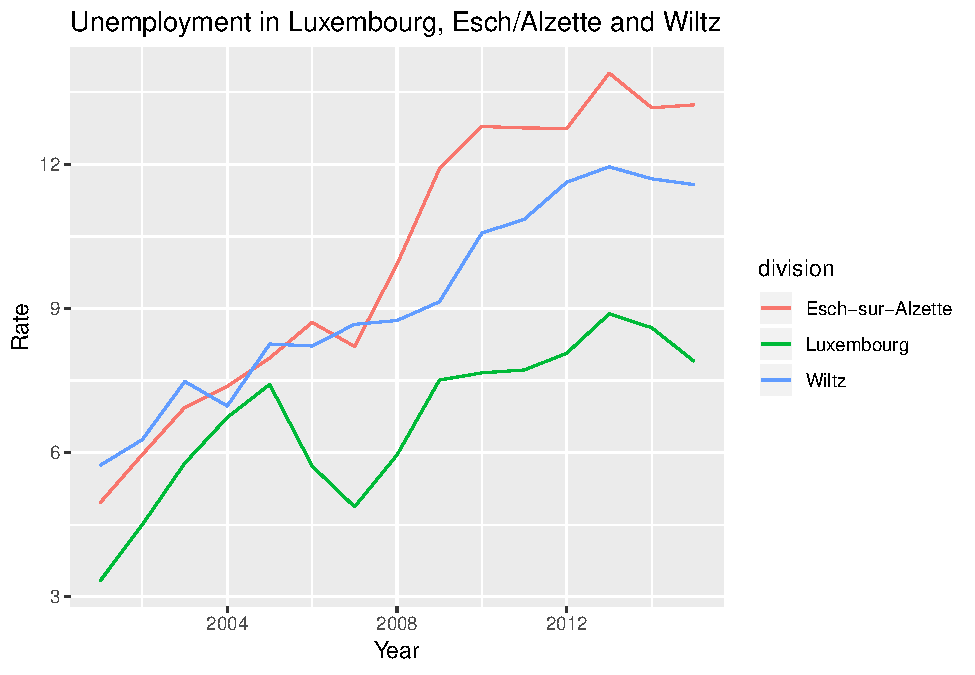
\includegraphics{modern_R_files/figure-latex/unnamed-chunk-305-1.pdf}

Because line plots are 2D, you need to specify the y and x axes. There
is also another option you need to add, \texttt{group\ =\ 1}. This is to
tell \texttt{aes()} that the dots have to be connected with a single
line. What if you want to plot more than one commune?

\begin{Shaded}
\begin{Highlighting}[]
\NormalTok{unemp_lux_data }\OperatorTok
\StringTok{  }\KeywordTok{filter}\NormalTok{(division }\OperatorTok{==}\StringTok{ "Luxembourg"} \OperatorTok{|}\StringTok{ }\NormalTok{division }\OperatorTok{==}\StringTok{ "Esch-sur-Alzette"}\NormalTok{) }\OperatorTok
\StringTok{  }\KeywordTok{ggplot}\NormalTok{(}\KeywordTok{aes}\NormalTok{(year, unemployment_rate_in_percent, }\DataTypeTok{group =}\NormalTok{ division, }\DataTypeTok{colour =}\NormalTok{ division)) }\OperatorTok{+}
\StringTok{  }\KeywordTok{geom_line}\NormalTok{()}
\end{Highlighting}
\end{Shaded}

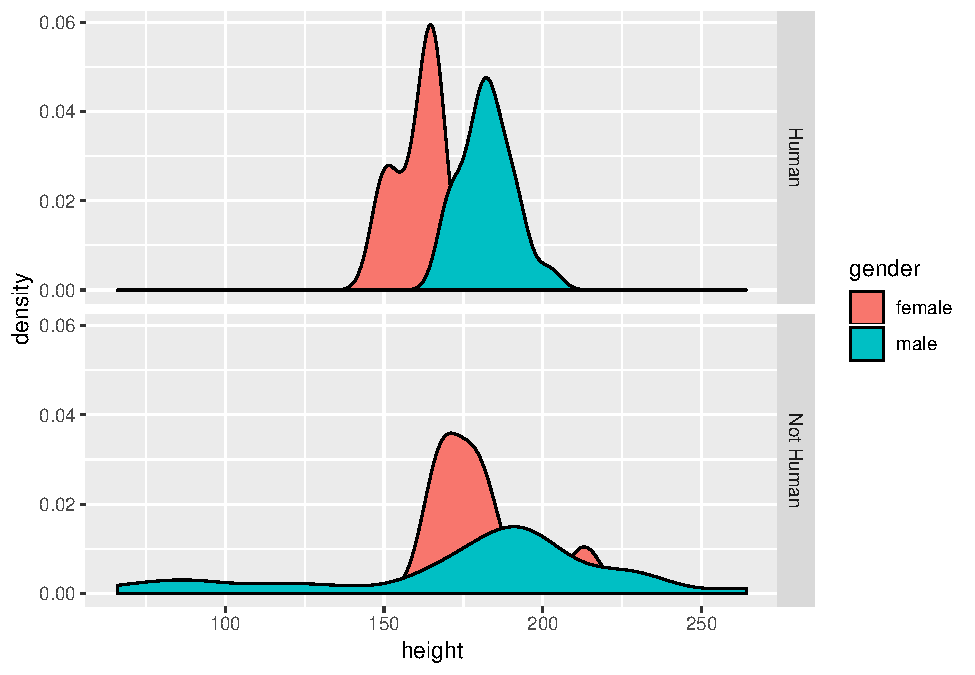
\includegraphics{modern_R_files/figure-latex/unnamed-chunk-306-1.pdf}

This time, I've specified \texttt{group\ =\ division} which means that
there has to be one line per as many communes as in the variable
\texttt{division}. I do the same for colours. I think the next example
illustrates how \texttt{ggplot2} is actually brilliant; if you need to
add a third commune, there is no need to specify anything else; no need
to add anything to the legend, no need to specify a third colour etc:

\begin{Shaded}
\begin{Highlighting}[]
\NormalTok{unemp_lux_data }\OperatorTok
\StringTok{  }\KeywordTok{filter}\NormalTok{(division }\OperatorTok\StringTok{ }\KeywordTok{c}\NormalTok{(}\StringTok{"Luxembourg"}\NormalTok{, }\StringTok{"Esch-sur-Alzette"}\NormalTok{, }\StringTok{"Wiltz"}\NormalTok{)) }\OperatorTok
\StringTok{  }\KeywordTok{ggplot}\NormalTok{(}\KeywordTok{aes}\NormalTok{(year, unemployment_rate_in_percent, }\DataTypeTok{group =}\NormalTok{ division, }\DataTypeTok{colour =}\NormalTok{ division)) }\OperatorTok{+}
\StringTok{  }\KeywordTok{geom_line}\NormalTok{()}
\end{Highlighting}
\end{Shaded}

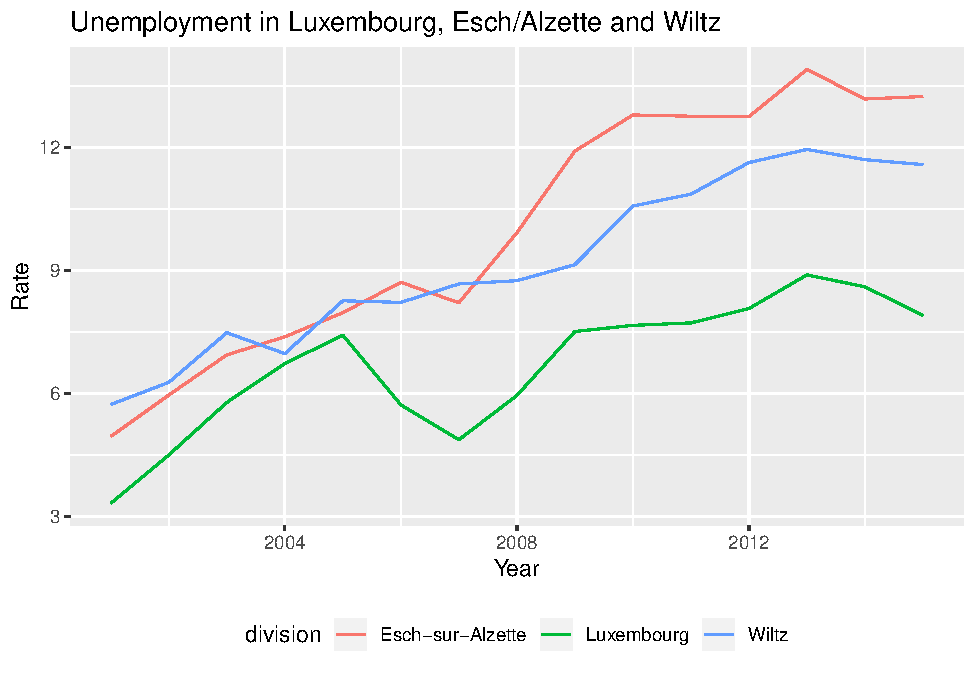
\includegraphics{modern_R_files/figure-latex/unnamed-chunk-307-1.pdf}

\hypertarget{facets}{%
\subsubsection{Facets}\label{facets}}

In some case you have a factor variable that separates the data you wish
to plot into different categories. If you want to have a plot per
category you can use the \texttt{facet\_grid()} function. Careful
though, this function does not take a variable as an argument, but a
formula, hence the \texttt{\textasciitilde{}} symbol in the code below:

\begin{Shaded}
\begin{Highlighting}[]
\NormalTok{starwars }\OperatorTok
\StringTok{  }\KeywordTok{mutate}\NormalTok{(}\DataTypeTok{human =} \KeywordTok{case_when}\NormalTok{(species }\OperatorTok{==}\StringTok{ "Human"} \OperatorTok{~}\StringTok{ "Human"}\NormalTok{,}
\NormalTok{                           species }\OperatorTok{!=}\StringTok{ "Human"} \OperatorTok{~}\StringTok{ "Not Human"}\NormalTok{)) }\OperatorTok
\StringTok{  }\KeywordTok{filter}\NormalTok{(gender }\OperatorTok\StringTok{ }\KeywordTok{c}\NormalTok{(}\StringTok{"female"}\NormalTok{, }\StringTok{"male"}\NormalTok{), }\OperatorTok{!}\KeywordTok{is.na}\NormalTok{(human)) }\OperatorTok
\StringTok{  }\KeywordTok{ggplot}\NormalTok{(}\KeywordTok{aes}\NormalTok{(height, }\DataTypeTok{fill =}\NormalTok{ gender)) }\OperatorTok{+}
\StringTok{  }\KeywordTok{facet_grid}\NormalTok{(. }\OperatorTok{~}\StringTok{ }\NormalTok{human) }\OperatorTok{+}\StringTok{ }\CommentTok{#<--- this is a formula}
\StringTok{  }\KeywordTok{geom_density}\NormalTok{()}
\end{Highlighting}
\end{Shaded}

\begin{verbatim}
## Warning: Removed 4 rows containing non-finite values (stat_density).
\end{verbatim}

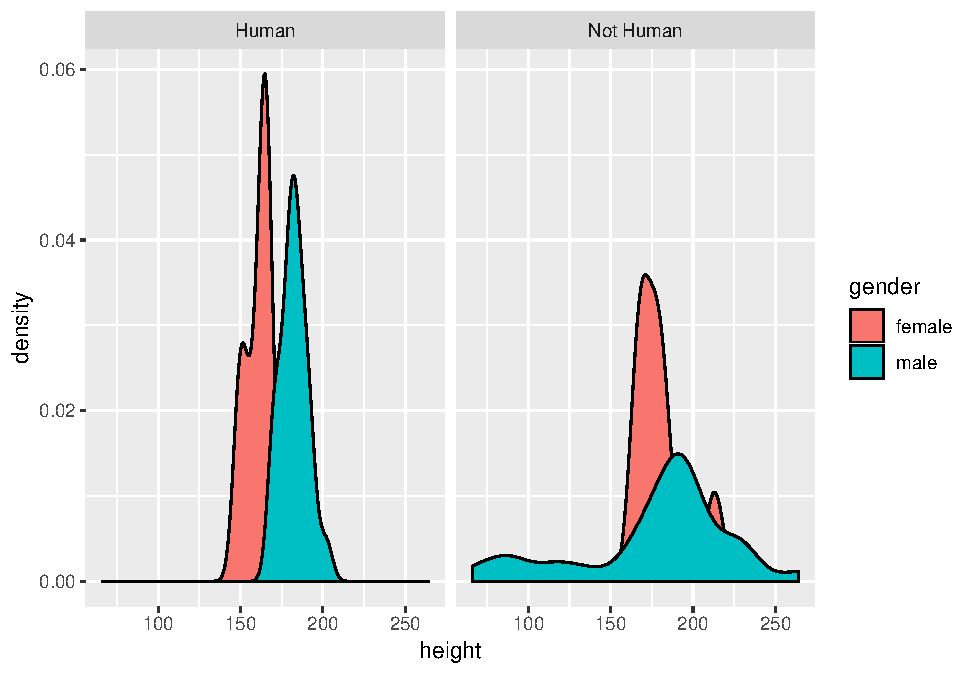
\includegraphics{modern_R_files/figure-latex/unnamed-chunk-308-1.pdf}

By changing the formula, you change how the facetting is done:

\begin{Shaded}
\begin{Highlighting}[]
\NormalTok{starwars }\OperatorTok
\StringTok{  }\KeywordTok{mutate}\NormalTok{(}\DataTypeTok{human =} \KeywordTok{case_when}\NormalTok{(species }\OperatorTok{==}\StringTok{ "Human"} \OperatorTok{~}\StringTok{ "Human"}\NormalTok{,}
\NormalTok{                           species }\OperatorTok{!=}\StringTok{ "Human"} \OperatorTok{~}\StringTok{ "Not Human"}\NormalTok{)) }\OperatorTok
\StringTok{  }\KeywordTok{filter}\NormalTok{(gender }\OperatorTok\StringTok{ }\KeywordTok{c}\NormalTok{(}\StringTok{"female"}\NormalTok{, }\StringTok{"male"}\NormalTok{), }\OperatorTok{!}\KeywordTok{is.na}\NormalTok{(human)) }\OperatorTok
\StringTok{  }\KeywordTok{ggplot}\NormalTok{(}\KeywordTok{aes}\NormalTok{(height, }\DataTypeTok{fill =}\NormalTok{ gender)) }\OperatorTok{+}
\StringTok{  }\KeywordTok{facet_grid}\NormalTok{(human }\OperatorTok{~}\StringTok{ }\NormalTok{.) }\OperatorTok{+}
\StringTok{  }\KeywordTok{geom_density}\NormalTok{()}
\end{Highlighting}
\end{Shaded}

\begin{verbatim}
## Warning: Removed 4 rows containing non-finite values (stat_density).
\end{verbatim}

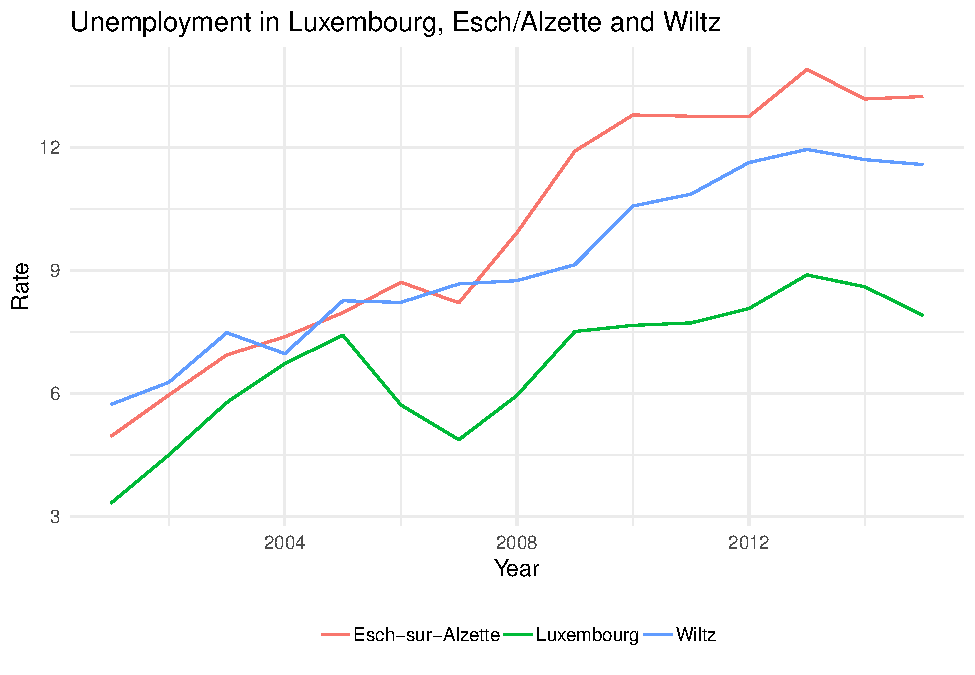
\includegraphics{modern_R_files/figure-latex/unnamed-chunk-309-1.pdf}

Recall the categorical variable \texttt{more\_1} that we computed in the
previous chapter? Let's use it as a faceting variable:

\begin{Shaded}
\begin{Highlighting}[]
\NormalTok{starwars }\OperatorTok
\StringTok{  }\KeywordTok{rowwise}\NormalTok{() }\OperatorTok
\StringTok{  }\KeywordTok{mutate}\NormalTok{(}\DataTypeTok{n_films =} \KeywordTok{length}\NormalTok{(films)) }\OperatorTok
\StringTok{  }\KeywordTok{mutate}\NormalTok{(}\DataTypeTok{more_1 =} \KeywordTok{case_when}\NormalTok{(n_films }\OperatorTok{==}\StringTok{ }\DecValTok{1} \OperatorTok{~}\StringTok{ "Exactly one movie"}\NormalTok{,}
\NormalTok{                            n_films }\OperatorTok{!=}\StringTok{ }\DecValTok{1} \OperatorTok{~}\StringTok{ "More than 1 movie"}\NormalTok{)) }\OperatorTok
\StringTok{  }\KeywordTok{mutate}\NormalTok{(}\DataTypeTok{human =} \KeywordTok{case_when}\NormalTok{(species }\OperatorTok{==}\StringTok{ "Human"} \OperatorTok{~}\StringTok{ "Human"}\NormalTok{,}
\NormalTok{                           species }\OperatorTok{!=}\StringTok{ "Human"} \OperatorTok{~}\StringTok{ "Not Human"}\NormalTok{)) }\OperatorTok
\StringTok{  }\KeywordTok{filter}\NormalTok{(gender }\OperatorTok\StringTok{ }\KeywordTok{c}\NormalTok{(}\StringTok{"female"}\NormalTok{, }\StringTok{"male"}\NormalTok{), }\OperatorTok{!}\KeywordTok{is.na}\NormalTok{(human)) }\OperatorTok
\StringTok{  }\KeywordTok{ggplot}\NormalTok{(}\KeywordTok{aes}\NormalTok{(height, }\DataTypeTok{fill =}\NormalTok{ gender)) }\OperatorTok{+}
\StringTok{  }\KeywordTok{facet_grid}\NormalTok{(human }\OperatorTok{~}\StringTok{ }\NormalTok{more_}\DecValTok{1}\NormalTok{) }\OperatorTok{+}
\StringTok{  }\KeywordTok{geom_density}\NormalTok{()}
\end{Highlighting}
\end{Shaded}

\begin{verbatim}
## Warning: Removed 4 rows containing non-finite values (stat_density).
\end{verbatim}

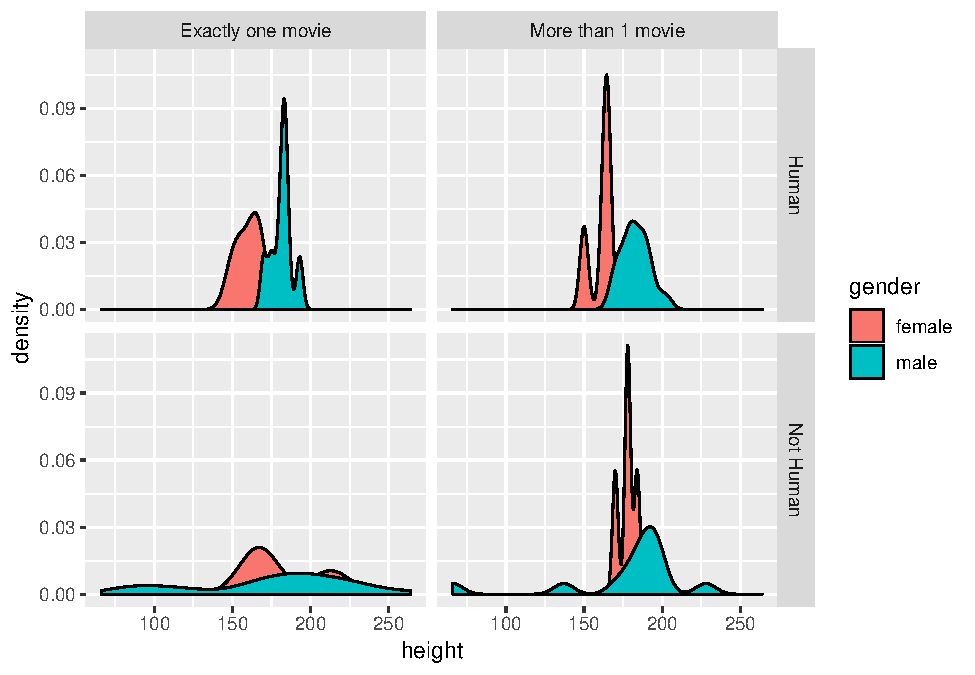
\includegraphics{modern_R_files/figure-latex/unnamed-chunk-310-1.pdf}

\hypertarget{pie-charts}{%
\subsubsection{Pie Charts}\label{pie-charts}}

I am not a huge fan of pie charts, but sometimes this is what you have
to do. So let's see how you can create pie charts. First, let's create a
mock dataset with the function \texttt{tibble::tribble()} which allows
you to create a dataset line by line:

\begin{Shaded}
\begin{Highlighting}[]
\NormalTok{test_data <-}\StringTok{ }\KeywordTok{tribble}\NormalTok{(}
  \OperatorTok{~}\NormalTok{id, }\OperatorTok{~}\NormalTok{var1, }\OperatorTok{~}\NormalTok{var2,  }\OperatorTok{~}\NormalTok{var3, }\OperatorTok{~}\NormalTok{var4, }\OperatorTok{~}\NormalTok{var5,}
  \StringTok{"a"}\NormalTok{, }\FloatTok{26.5}\NormalTok{, }\DecValTok{38}\NormalTok{, }\DecValTok{30}\NormalTok{, }\DecValTok{32}\NormalTok{, }\DecValTok{34}\NormalTok{,}
  \StringTok{"b"}\NormalTok{, }\DecValTok{30}\NormalTok{, }\DecValTok{30}\NormalTok{, }\DecValTok{28}\NormalTok{, }\DecValTok{32}\NormalTok{, }\DecValTok{30}\NormalTok{,}
  \StringTok{"c"}\NormalTok{, }\DecValTok{34}\NormalTok{, }\DecValTok{32}\NormalTok{, }\DecValTok{30}\NormalTok{, }\DecValTok{28}\NormalTok{, }\FloatTok{26.5}
\NormalTok{)}
\end{Highlighting}
\end{Shaded}

This data is not in the right format though, which is wide. We need to
have it in the long format for it to work with \texttt{ggplot2}. For
this, let's use \texttt{tidyr::gather()} as seen in the previous
chapter:

\begin{Shaded}
\begin{Highlighting}[]
\NormalTok{test_data_long =}\StringTok{ }\NormalTok{test_data }\OperatorTok
\StringTok{  }\KeywordTok{gather}\NormalTok{(variable, value, }\KeywordTok{starts_with}\NormalTok{(}\StringTok{"var"}\NormalTok{))}
\end{Highlighting}
\end{Shaded}

Now, let's plot this data, first by creating 3 bar plots:

\begin{Shaded}
\begin{Highlighting}[]
\KeywordTok{ggplot}\NormalTok{(test_data_long) }\OperatorTok{+}
\StringTok{  }\KeywordTok{facet_wrap}\NormalTok{(}\OperatorTok{~}\NormalTok{id) }\OperatorTok{+}
\StringTok{  }\KeywordTok{geom_bar}\NormalTok{(}\KeywordTok{aes}\NormalTok{(variable, value, }\DataTypeTok{fill =}\NormalTok{ variable), }\DataTypeTok{stat =} \StringTok{"identity"}\NormalTok{)}
\end{Highlighting}
\end{Shaded}

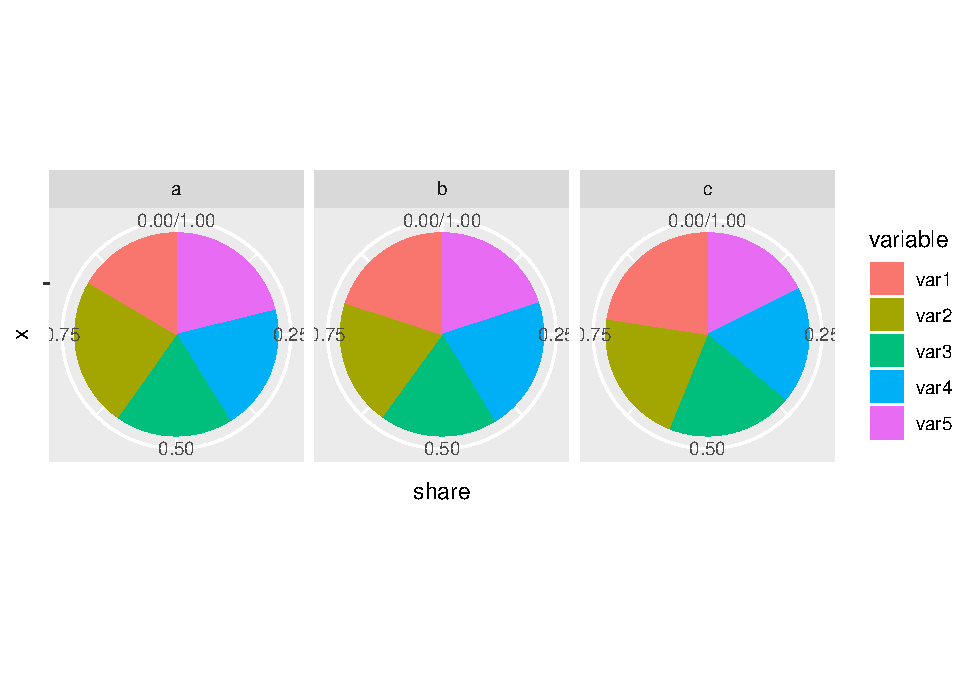
\includegraphics{modern_R_files/figure-latex/unnamed-chunk-313-1.pdf}

In the code above, I introduce a new option, called
\texttt{stat\ =\ "identity"}. By default, \texttt{geom\_bar()} counts
the number of observations of each category that is plotted, which is a
statistical transformation. By adding \texttt{stat\ =\ "identity"}, I
force the statistical transformation to be the identity function, and
thus plot the data as is.

To create the pie chart, first we need to compute the share of each
\texttt{id} to \texttt{var1}, \texttt{var2}, etc\ldots{}

To do this, we first group by \texttt{id}, then compute the total. Then
we use a new function \texttt{ungroup()}. After using \texttt{ungroup()}
all the computations are done on the whole dataset instead of by group,
which is what we need to compute the share:

\begin{Shaded}
\begin{Highlighting}[]
\NormalTok{test_data_long =}\StringTok{ }\NormalTok{test_data_long }\OperatorTok
\StringTok{  }\KeywordTok{group_by}\NormalTok{(id) }\OperatorTok
\StringTok{  }\KeywordTok{mutate}\NormalTok{(}\DataTypeTok{total =} \KeywordTok{sum}\NormalTok{(value)) }\OperatorTok
\StringTok{  }\KeywordTok{ungroup}\NormalTok{() }\OperatorTok
\StringTok{  }\KeywordTok{mutate}\NormalTok{(}\DataTypeTok{share =}\NormalTok{ value}\OperatorTok{/}\NormalTok{total)}
\end{Highlighting}
\end{Shaded}

Let's take a look to see if this is what we wanted:

\begin{Shaded}
\begin{Highlighting}[]
\KeywordTok{print}\NormalTok{(test_data_long)}
\end{Highlighting}
\end{Shaded}

\begin{verbatim}
## # A tibble: 15 x 5
##    id    variable value total share
##    <chr> <chr>    <dbl> <dbl> <dbl>
##  1 a     var1      26.5  160. 0.165
##  2 b     var1      30    150  0.2  
##  3 c     var1      34    150. 0.226
##  4 a     var2      38    160. 0.237
##  5 b     var2      30    150  0.2  
##  6 c     var2      32    150. 0.213
##  7 a     var3      30    160. 0.187
##  8 b     var3      28    150  0.187
##  9 c     var3      30    150. 0.199
## 10 a     var4      32    160. 0.199
## 11 b     var4      32    150  0.213
## 12 c     var4      28    150. 0.186
## 13 a     var5      34    160. 0.212
## 14 b     var5      30    150  0.2  
## 15 c     var5      26.5  150. 0.176
\end{verbatim}

If you didn't understand what \texttt{ungroup()} did, rerun the last few
lines with it and inspect the output.

To plot the pie chart, we create a barplot again, but specify polar
coordinates:

\begin{Shaded}
\begin{Highlighting}[]
\KeywordTok{ggplot}\NormalTok{(test_data_long) }\OperatorTok{+}
\StringTok{  }\KeywordTok{facet_wrap}\NormalTok{(}\OperatorTok{~}\NormalTok{id) }\OperatorTok{+}
\StringTok{  }\KeywordTok{geom_bar}\NormalTok{(}\KeywordTok{aes}\NormalTok{(}\DataTypeTok{y =}\NormalTok{ share, }\DataTypeTok{x =} \StringTok{""}\NormalTok{, }\DataTypeTok{fill =}\NormalTok{ variable), }\DataTypeTok{stat =} \StringTok{"identity"}\NormalTok{) }\OperatorTok{+}
\StringTok{  }\KeywordTok{theme}\NormalTok{() }\OperatorTok{+}
\StringTok{  }\KeywordTok{coord_polar}\NormalTok{(}\StringTok{"y"}\NormalTok{, }\DataTypeTok{start =} \DecValTok{0}\NormalTok{)}
\end{Highlighting}
\end{Shaded}

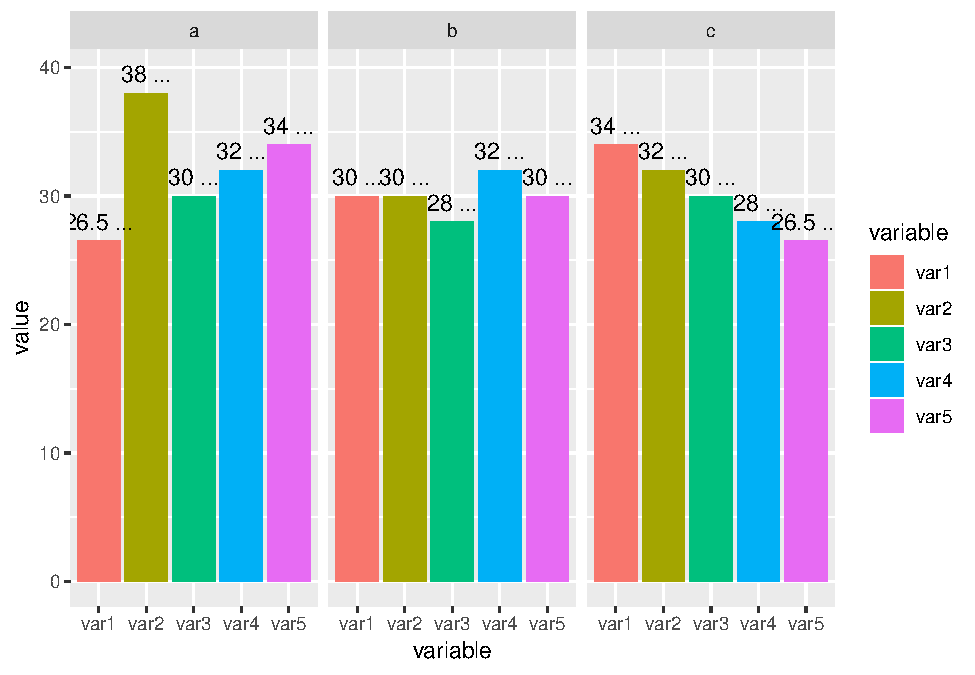
\includegraphics{modern_R_files/figure-latex/unnamed-chunk-316-1.pdf}

As you can see, this typical pie chart is not very easy to read;
compared to the barplots above it is not easy to distinguish \texttt{a}
from \texttt{b} from \texttt{c}. It is possible to amend the pie chart a
bit to make it clearer, by specifying \texttt{variable} as the
\texttt{x}:

\begin{Shaded}
\begin{Highlighting}[]
\KeywordTok{ggplot}\NormalTok{(test_data_long) }\OperatorTok{+}
\StringTok{  }\KeywordTok{facet_wrap}\NormalTok{(}\OperatorTok{~}\NormalTok{id) }\OperatorTok{+}
\StringTok{  }\KeywordTok{geom_bar}\NormalTok{(}\KeywordTok{aes}\NormalTok{(}\DataTypeTok{y =}\NormalTok{ share, }\DataTypeTok{x =}\NormalTok{ variable, }\DataTypeTok{fill =}\NormalTok{ variable), }\DataTypeTok{stat =} \StringTok{"identity"}\NormalTok{) }\OperatorTok{+}
\StringTok{  }\KeywordTok{theme}\NormalTok{() }\OperatorTok{+}
\StringTok{  }\KeywordTok{coord_polar}\NormalTok{(}\StringTok{"x"}\NormalTok{, }\DataTypeTok{start =} \DecValTok{0}\NormalTok{)}
\end{Highlighting}
\end{Shaded}

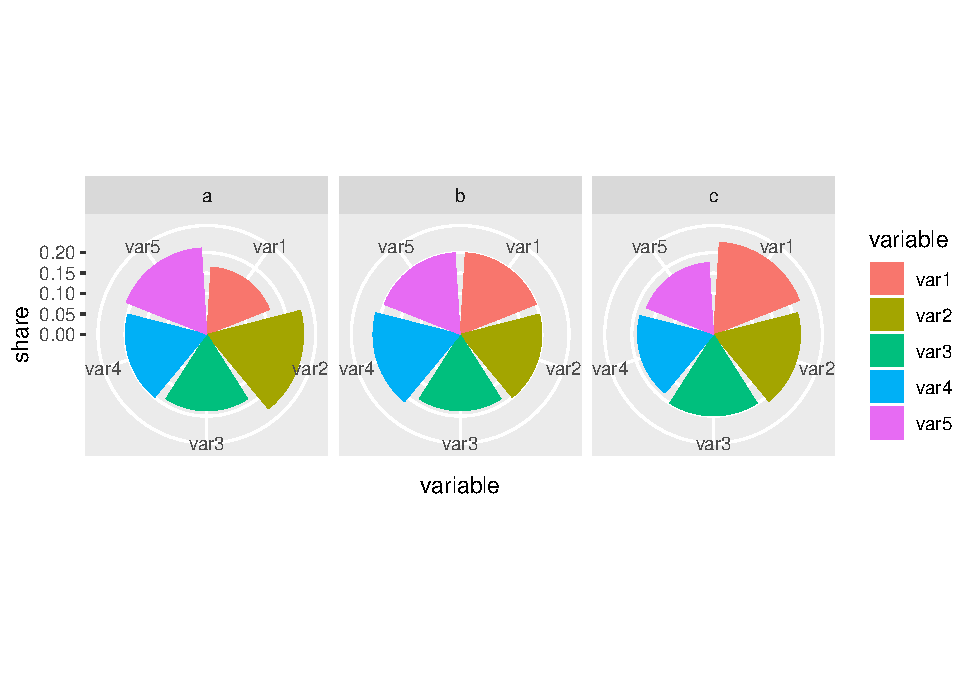
\includegraphics{modern_R_files/figure-latex/unnamed-chunk-317-1.pdf}

But as a general rule, avoid pie charts if possible. Barplots show the
same information, much, much clearer.

\hypertarget{adding-text-to-plots}{%
\subsubsection{Adding text to plots}\label{adding-text-to-plots}}

Sometimes you might want to add some text to your plots. This is
possible with \texttt{geom\_text()}:

\begin{Shaded}
\begin{Highlighting}[]
\KeywordTok{ggplot}\NormalTok{(test_data_long) }\OperatorTok{+}
\StringTok{  }\KeywordTok{facet_wrap}\NormalTok{(}\OperatorTok{~}\NormalTok{id) }\OperatorTok{+}
\StringTok{  }\KeywordTok{geom_bar}\NormalTok{(}\KeywordTok{aes}\NormalTok{(variable, value, }\DataTypeTok{fill =}\NormalTok{ variable), }\DataTypeTok{stat =} \StringTok{"identity"}\NormalTok{) }\OperatorTok{+}
\StringTok{  }\KeywordTok{geom_text}\NormalTok{(}\KeywordTok{aes}\NormalTok{(variable, value }\OperatorTok{+}\StringTok{ }\FloatTok{1.5}\NormalTok{, }\DataTypeTok{label =}\NormalTok{ value))}
\end{Highlighting}
\end{Shaded}

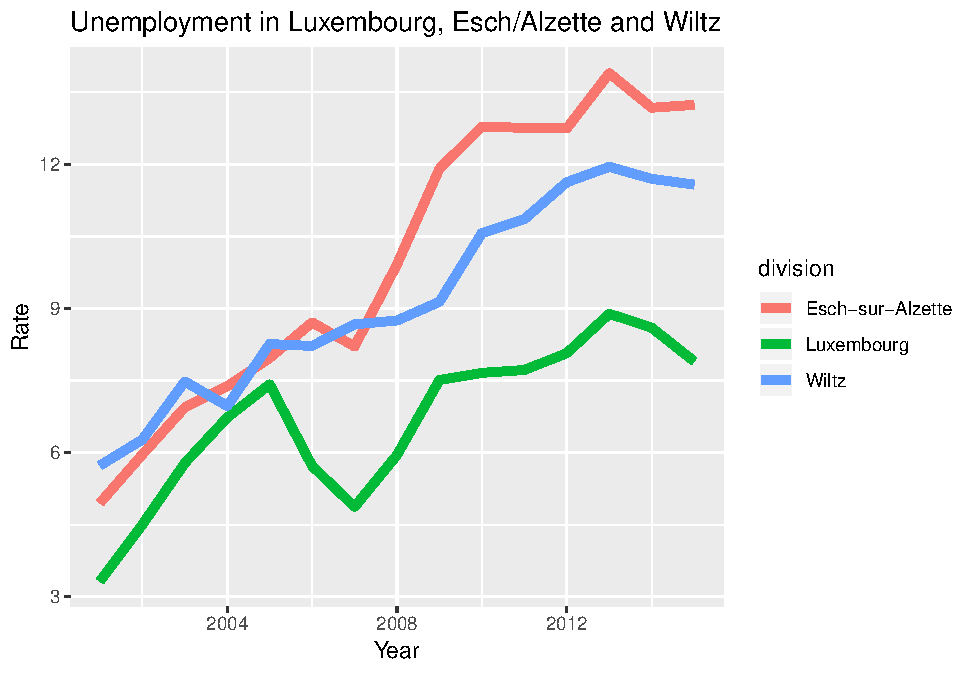
\includegraphics{modern_R_files/figure-latex/unnamed-chunk-318-1.pdf}

You can put anything after \texttt{label\ =}but in general what you'd
want are the values, so that's what I put there. But you can also refine
it, imagine the values are actualy, say €:

\begin{Shaded}
\begin{Highlighting}[]
\KeywordTok{ggplot}\NormalTok{(test_data_long) }\OperatorTok{+}
\StringTok{  }\KeywordTok{facet_wrap}\NormalTok{(}\OperatorTok{~}\NormalTok{id) }\OperatorTok{+}
\StringTok{  }\KeywordTok{geom_bar}\NormalTok{(}\KeywordTok{aes}\NormalTok{(variable, value, }\DataTypeTok{fill =}\NormalTok{ variable), }\DataTypeTok{stat =} \StringTok{"identity"}\NormalTok{) }\OperatorTok{+}
\StringTok{  }\KeywordTok{geom_text}\NormalTok{(}\KeywordTok{aes}\NormalTok{(variable, value }\OperatorTok{+}\StringTok{ }\FloatTok{1.5}\NormalTok{, }\DataTypeTok{label =} \KeywordTok{paste}\NormalTok{(value, }\StringTok{"€"}\NormalTok{)))}
\end{Highlighting}
\end{Shaded}

\begin{verbatim}
## Warning in grid.Call.graphics(C_text, as.graphicsAnnot(x$label), x$x,
## x$y, : conversion failure on '26.5 €' in 'mbcsToSbcs': dot substituted for
## <e2>
\end{verbatim}

\begin{verbatim}
## Warning in grid.Call.graphics(C_text, as.graphicsAnnot(x$label), x$x,
## x$y, : conversion failure on '26.5 €' in 'mbcsToSbcs': dot substituted for
## <82>
\end{verbatim}

\begin{verbatim}
## Warning in grid.Call.graphics(C_text, as.graphicsAnnot(x$label), x$x,
## x$y, : conversion failure on '26.5 €' in 'mbcsToSbcs': dot substituted for
## <ac>
\end{verbatim}

\begin{verbatim}
## Warning in grid.Call.graphics(C_text, as.graphicsAnnot(x$label), x$x,
## x$y, : conversion failure on '38 €' in 'mbcsToSbcs': dot substituted for
## <e2>
\end{verbatim}

\begin{verbatim}
## Warning in grid.Call.graphics(C_text, as.graphicsAnnot(x$label), x$x,
## x$y, : conversion failure on '38 €' in 'mbcsToSbcs': dot substituted for
## <82>
\end{verbatim}

\begin{verbatim}
## Warning in grid.Call.graphics(C_text, as.graphicsAnnot(x$label), x$x,
## x$y, : conversion failure on '38 €' in 'mbcsToSbcs': dot substituted for
## <ac>
\end{verbatim}

\begin{verbatim}
## Warning in grid.Call.graphics(C_text, as.graphicsAnnot(x$label), x$x,
## x$y, : conversion failure on '30 €' in 'mbcsToSbcs': dot substituted for
## <e2>
\end{verbatim}

\begin{verbatim}
## Warning in grid.Call.graphics(C_text, as.graphicsAnnot(x$label), x$x,
## x$y, : conversion failure on '30 €' in 'mbcsToSbcs': dot substituted for
## <82>
\end{verbatim}

\begin{verbatim}
## Warning in grid.Call.graphics(C_text, as.graphicsAnnot(x$label), x$x,
## x$y, : conversion failure on '30 €' in 'mbcsToSbcs': dot substituted for
## <ac>
\end{verbatim}

\begin{verbatim}
## Warning in grid.Call.graphics(C_text, as.graphicsAnnot(x$label), x$x,
## x$y, : conversion failure on '32 €' in 'mbcsToSbcs': dot substituted for
## <e2>
\end{verbatim}

\begin{verbatim}
## Warning in grid.Call.graphics(C_text, as.graphicsAnnot(x$label), x$x,
## x$y, : conversion failure on '32 €' in 'mbcsToSbcs': dot substituted for
## <82>
\end{verbatim}

\begin{verbatim}
## Warning in grid.Call.graphics(C_text, as.graphicsAnnot(x$label), x$x,
## x$y, : conversion failure on '32 €' in 'mbcsToSbcs': dot substituted for
## <ac>
\end{verbatim}

\begin{verbatim}
## Warning in grid.Call.graphics(C_text, as.graphicsAnnot(x$label), x$x,
## x$y, : conversion failure on '34 €' in 'mbcsToSbcs': dot substituted for
## <e2>
\end{verbatim}

\begin{verbatim}
## Warning in grid.Call.graphics(C_text, as.graphicsAnnot(x$label), x$x,
## x$y, : conversion failure on '34 €' in 'mbcsToSbcs': dot substituted for
## <82>
\end{verbatim}

\begin{verbatim}
## Warning in grid.Call.graphics(C_text, as.graphicsAnnot(x$label), x$x,
## x$y, : conversion failure on '34 €' in 'mbcsToSbcs': dot substituted for
## <ac>
\end{verbatim}

\begin{verbatim}
## Warning in grid.Call.graphics(C_text, as.graphicsAnnot(x$label), x$x,
## x$y, : conversion failure on '30 €' in 'mbcsToSbcs': dot substituted for
## <e2>
\end{verbatim}

\begin{verbatim}
## Warning in grid.Call.graphics(C_text, as.graphicsAnnot(x$label), x$x,
## x$y, : conversion failure on '30 €' in 'mbcsToSbcs': dot substituted for
## <82>
\end{verbatim}

\begin{verbatim}
## Warning in grid.Call.graphics(C_text, as.graphicsAnnot(x$label), x$x,
## x$y, : conversion failure on '30 €' in 'mbcsToSbcs': dot substituted for
## <ac>
\end{verbatim}

\begin{verbatim}
## Warning in grid.Call.graphics(C_text, as.graphicsAnnot(x$label), x$x,
## x$y, : conversion failure on '30 €' in 'mbcsToSbcs': dot substituted for
## <e2>
\end{verbatim}

\begin{verbatim}
## Warning in grid.Call.graphics(C_text, as.graphicsAnnot(x$label), x$x,
## x$y, : conversion failure on '30 €' in 'mbcsToSbcs': dot substituted for
## <82>
\end{verbatim}

\begin{verbatim}
## Warning in grid.Call.graphics(C_text, as.graphicsAnnot(x$label), x$x,
## x$y, : conversion failure on '30 €' in 'mbcsToSbcs': dot substituted for
## <ac>
\end{verbatim}

\begin{verbatim}
## Warning in grid.Call.graphics(C_text, as.graphicsAnnot(x$label), x$x,
## x$y, : conversion failure on '28 €' in 'mbcsToSbcs': dot substituted for
## <e2>
\end{verbatim}

\begin{verbatim}
## Warning in grid.Call.graphics(C_text, as.graphicsAnnot(x$label), x$x,
## x$y, : conversion failure on '28 €' in 'mbcsToSbcs': dot substituted for
## <82>
\end{verbatim}

\begin{verbatim}
## Warning in grid.Call.graphics(C_text, as.graphicsAnnot(x$label), x$x,
## x$y, : conversion failure on '28 €' in 'mbcsToSbcs': dot substituted for
## <ac>
\end{verbatim}

\begin{verbatim}
## Warning in grid.Call.graphics(C_text, as.graphicsAnnot(x$label), x$x,
## x$y, : conversion failure on '32 €' in 'mbcsToSbcs': dot substituted for
## <e2>
\end{verbatim}

\begin{verbatim}
## Warning in grid.Call.graphics(C_text, as.graphicsAnnot(x$label), x$x,
## x$y, : conversion failure on '32 €' in 'mbcsToSbcs': dot substituted for
## <82>
\end{verbatim}

\begin{verbatim}
## Warning in grid.Call.graphics(C_text, as.graphicsAnnot(x$label), x$x,
## x$y, : conversion failure on '32 €' in 'mbcsToSbcs': dot substituted for
## <ac>
\end{verbatim}

\begin{verbatim}
## Warning in grid.Call.graphics(C_text, as.graphicsAnnot(x$label), x$x,
## x$y, : conversion failure on '30 €' in 'mbcsToSbcs': dot substituted for
## <e2>
\end{verbatim}

\begin{verbatim}
## Warning in grid.Call.graphics(C_text, as.graphicsAnnot(x$label), x$x,
## x$y, : conversion failure on '30 €' in 'mbcsToSbcs': dot substituted for
## <82>
\end{verbatim}

\begin{verbatim}
## Warning in grid.Call.graphics(C_text, as.graphicsAnnot(x$label), x$x,
## x$y, : conversion failure on '30 €' in 'mbcsToSbcs': dot substituted for
## <ac>
\end{verbatim}

\begin{verbatim}
## Warning in grid.Call.graphics(C_text, as.graphicsAnnot(x$label), x$x,
## x$y, : conversion failure on '34 €' in 'mbcsToSbcs': dot substituted for
## <e2>
\end{verbatim}

\begin{verbatim}
## Warning in grid.Call.graphics(C_text, as.graphicsAnnot(x$label), x$x,
## x$y, : conversion failure on '34 €' in 'mbcsToSbcs': dot substituted for
## <82>
\end{verbatim}

\begin{verbatim}
## Warning in grid.Call.graphics(C_text, as.graphicsAnnot(x$label), x$x,
## x$y, : conversion failure on '34 €' in 'mbcsToSbcs': dot substituted for
## <ac>
\end{verbatim}

\begin{verbatim}
## Warning in grid.Call.graphics(C_text, as.graphicsAnnot(x$label), x$x,
## x$y, : conversion failure on '32 €' in 'mbcsToSbcs': dot substituted for
## <e2>
\end{verbatim}

\begin{verbatim}
## Warning in grid.Call.graphics(C_text, as.graphicsAnnot(x$label), x$x,
## x$y, : conversion failure on '32 €' in 'mbcsToSbcs': dot substituted for
## <82>
\end{verbatim}

\begin{verbatim}
## Warning in grid.Call.graphics(C_text, as.graphicsAnnot(x$label), x$x,
## x$y, : conversion failure on '32 €' in 'mbcsToSbcs': dot substituted for
## <ac>
\end{verbatim}

\begin{verbatim}
## Warning in grid.Call.graphics(C_text, as.graphicsAnnot(x$label), x$x,
## x$y, : conversion failure on '30 €' in 'mbcsToSbcs': dot substituted for
## <e2>
\end{verbatim}

\begin{verbatim}
## Warning in grid.Call.graphics(C_text, as.graphicsAnnot(x$label), x$x,
## x$y, : conversion failure on '30 €' in 'mbcsToSbcs': dot substituted for
## <82>
\end{verbatim}

\begin{verbatim}
## Warning in grid.Call.graphics(C_text, as.graphicsAnnot(x$label), x$x,
## x$y, : conversion failure on '30 €' in 'mbcsToSbcs': dot substituted for
## <ac>
\end{verbatim}

\begin{verbatim}
## Warning in grid.Call.graphics(C_text, as.graphicsAnnot(x$label), x$x,
## x$y, : conversion failure on '28 €' in 'mbcsToSbcs': dot substituted for
## <e2>
\end{verbatim}

\begin{verbatim}
## Warning in grid.Call.graphics(C_text, as.graphicsAnnot(x$label), x$x,
## x$y, : conversion failure on '28 €' in 'mbcsToSbcs': dot substituted for
## <82>
\end{verbatim}

\begin{verbatim}
## Warning in grid.Call.graphics(C_text, as.graphicsAnnot(x$label), x$x,
## x$y, : conversion failure on '28 €' in 'mbcsToSbcs': dot substituted for
## <ac>
\end{verbatim}

\begin{verbatim}
## Warning in grid.Call.graphics(C_text, as.graphicsAnnot(x$label), x$x,
## x$y, : conversion failure on '26.5 €' in 'mbcsToSbcs': dot substituted for
## <e2>
\end{verbatim}

\begin{verbatim}
## Warning in grid.Call.graphics(C_text, as.graphicsAnnot(x$label), x$x,
## x$y, : conversion failure on '26.5 €' in 'mbcsToSbcs': dot substituted for
## <82>
\end{verbatim}

\begin{verbatim}
## Warning in grid.Call.graphics(C_text, as.graphicsAnnot(x$label), x$x,
## x$y, : conversion failure on '26.5 €' in 'mbcsToSbcs': dot substituted for
## <ac>
\end{verbatim}

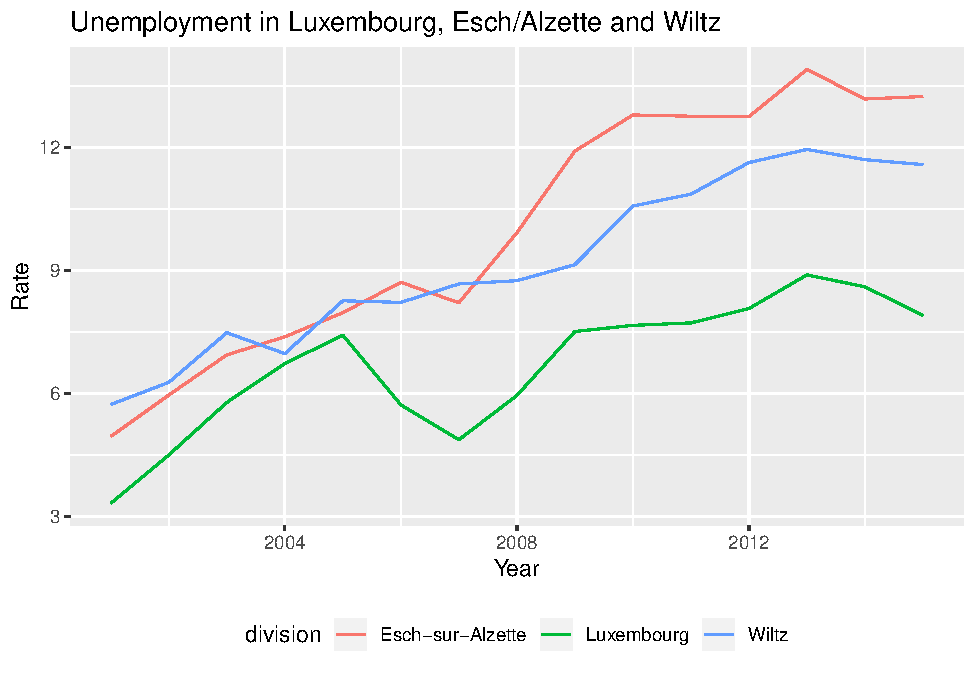
\includegraphics{modern_R_files/figure-latex/unnamed-chunk-319-1.pdf}

\hypertarget{customization}{%
\subsection{Customization}\label{customization}}

Every plot you've seen until now was made with the default look of
\texttt{ggplot2}. If you want to change the look, you can apply a theme,
and a colour scheme. Let's take a look at themes first by using the ones
found in the package \texttt{ggthemes}. But first, let's learn how to
change the names of the axes and how to title a plot.

\hypertarget{titles-axes-names-and-more}{%
\subsubsection{Titles, axes names and
more}\label{titles-axes-names-and-more}}

To change the title of the plot, and of the axes, you need to pass the
names to the \texttt{labs()} function:

\begin{Shaded}
\begin{Highlighting}[]
\NormalTok{unemp_lux_data }\OperatorTok
\StringTok{  }\KeywordTok{filter}\NormalTok{(division }\OperatorTok\StringTok{ }\KeywordTok{c}\NormalTok{(}\StringTok{"Luxembourg"}\NormalTok{, }\StringTok{"Esch-sur-Alzette"}\NormalTok{, }\StringTok{"Wiltz"}\NormalTok{)) }\OperatorTok
\StringTok{  }\KeywordTok{ggplot}\NormalTok{(}\KeywordTok{aes}\NormalTok{(year, unemployment_rate_in_percent, }\DataTypeTok{group =}\NormalTok{ division, }\DataTypeTok{colour =}\NormalTok{ division)) }\OperatorTok{+}
\StringTok{  }\KeywordTok{labs}\NormalTok{(}\DataTypeTok{title =} \StringTok{"Unemployment in Luxembourg, Esch/Alzette and Wiltz"}\NormalTok{, }\DataTypeTok{x =} \StringTok{"Year"}\NormalTok{, }\DataTypeTok{y =} \StringTok{"Rate"}\NormalTok{) }\OperatorTok{+}
\StringTok{  }\KeywordTok{geom_line}\NormalTok{()}
\end{Highlighting}
\end{Shaded}

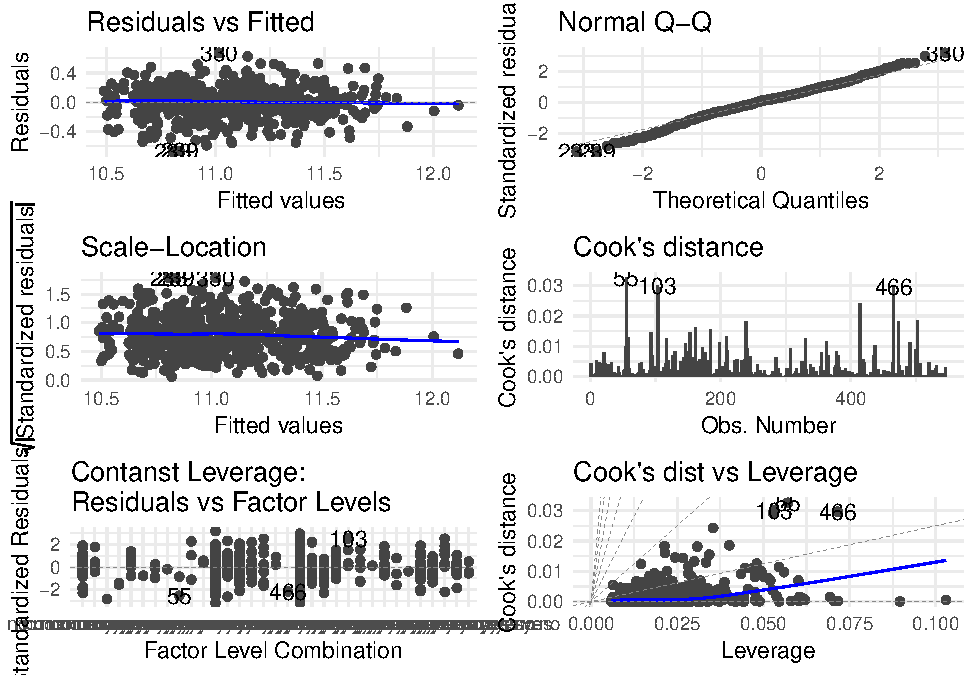
\includegraphics{modern_R_files/figure-latex/unnamed-chunk-320-1.pdf}

What if you want to make the lines thicker?

\begin{Shaded}
\begin{Highlighting}[]
\NormalTok{unemp_lux_data }\OperatorTok
\StringTok{  }\KeywordTok{filter}\NormalTok{(division }\OperatorTok\StringTok{ }\KeywordTok{c}\NormalTok{(}\StringTok{"Luxembourg"}\NormalTok{, }\StringTok{"Esch-sur-Alzette"}\NormalTok{, }\StringTok{"Wiltz"}\NormalTok{)) }\OperatorTok
\StringTok{  }\KeywordTok{ggplot}\NormalTok{(}\KeywordTok{aes}\NormalTok{(year, unemployment_rate_in_percent, }\DataTypeTok{group =}\NormalTok{ division, }\DataTypeTok{colour =}\NormalTok{ division)) }\OperatorTok{+}
\StringTok{  }\KeywordTok{labs}\NormalTok{(}\DataTypeTok{title =} \StringTok{"Unemployment in Luxembourg, Esch/Alzette and Wiltz"}\NormalTok{, }\DataTypeTok{x =} \StringTok{"Year"}\NormalTok{, }\DataTypeTok{y =} \StringTok{"Rate"}\NormalTok{) }\OperatorTok{+}
\StringTok{  }\KeywordTok{geom_line}\NormalTok{(}\DataTypeTok{size =} \DecValTok{2}\NormalTok{)}
\end{Highlighting}
\end{Shaded}

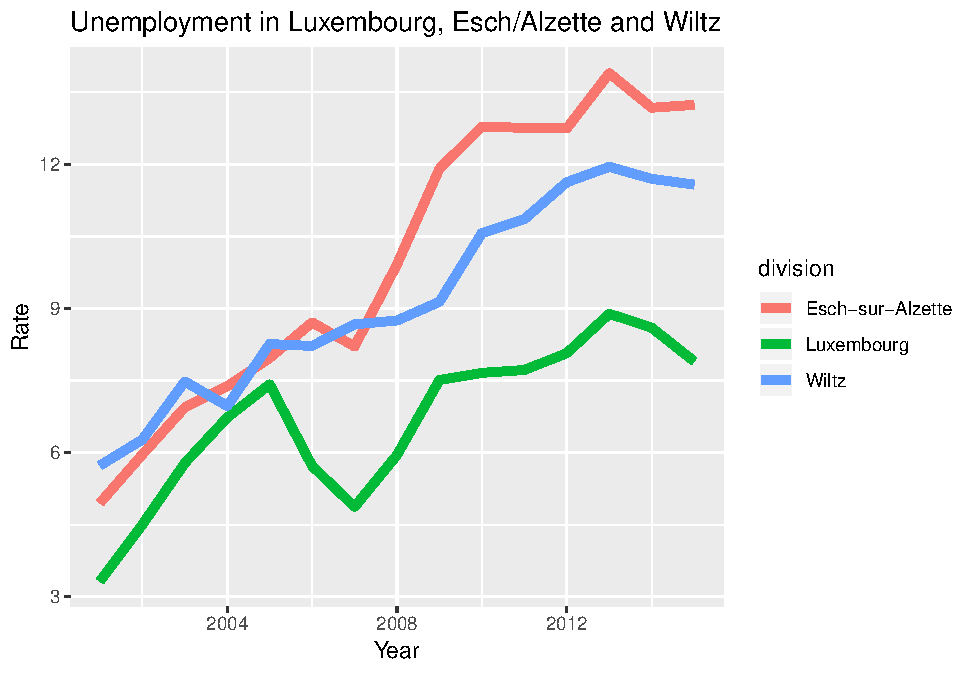
\includegraphics{modern_R_files/figure-latex/unnamed-chunk-321-1.pdf}

\hypertarget{themes}{%
\subsubsection{Themes}\label{themes}}

Let's go back to the unemployment line plots. For now, let's keep the
base \texttt{ggplot2} theme, but modify it a bit. For example, the
legend placement is actually a feature of the theme. This means that if
you want to change where the legend is placed you need to modify this
feature from the theme. This is done with the function \texttt{theme()}:

\begin{Shaded}
\begin{Highlighting}[]
\NormalTok{unemp_lux_data }\OperatorTok
\StringTok{  }\KeywordTok{filter}\NormalTok{(division }\OperatorTok\StringTok{ }\KeywordTok{c}\NormalTok{(}\StringTok{"Luxembourg"}\NormalTok{, }\StringTok{"Esch-sur-Alzette"}\NormalTok{, }\StringTok{"Wiltz"}\NormalTok{)) }\OperatorTok
\StringTok{  }\KeywordTok{ggplot}\NormalTok{(}\KeywordTok{aes}\NormalTok{(year, unemployment_rate_in_percent, }\DataTypeTok{group =}\NormalTok{ division, }\DataTypeTok{colour =}\NormalTok{ division)) }\OperatorTok{+}
\StringTok{  }\KeywordTok{theme}\NormalTok{(}\DataTypeTok{legend.position =} \StringTok{"bottom"}\NormalTok{) }\OperatorTok{+}
\StringTok{  }\KeywordTok{labs}\NormalTok{(}\DataTypeTok{title =} \StringTok{"Unemployment in Luxembourg, Esch/Alzette and Wiltz"}\NormalTok{, }\DataTypeTok{x =} \StringTok{"Year"}\NormalTok{, }\DataTypeTok{y =} \StringTok{"Rate"}\NormalTok{)}\OperatorTok{+}
\StringTok{  }\KeywordTok{geom_line}\NormalTok{()}
\end{Highlighting}
\end{Shaded}

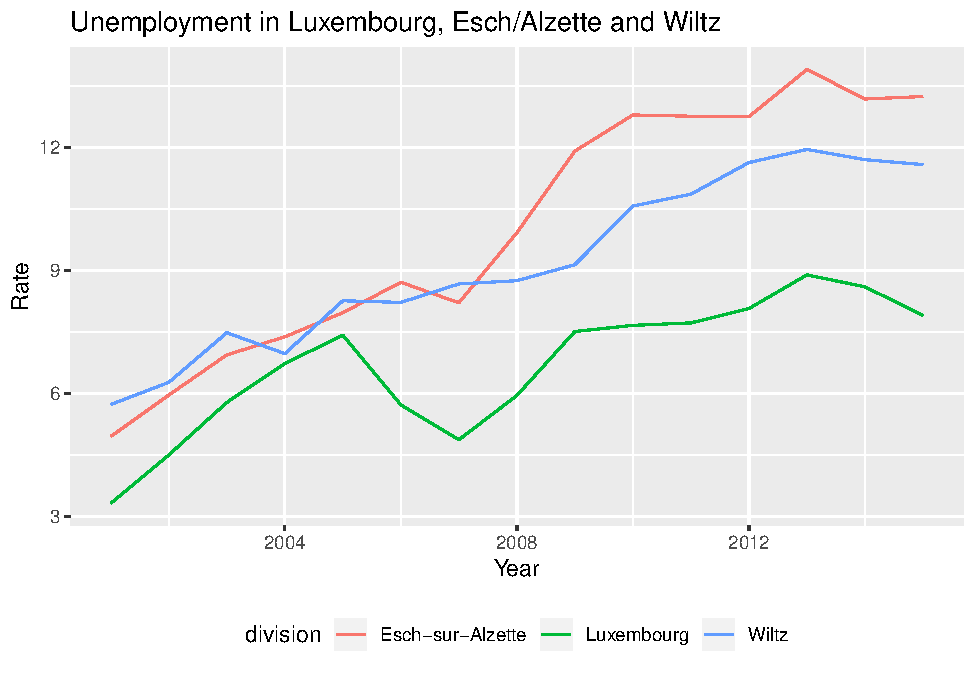
\includegraphics{modern_R_files/figure-latex/unnamed-chunk-322-1.pdf}

What I also like to do is remove the title of the legend, because it is
often superfluous:

\begin{Shaded}
\begin{Highlighting}[]
\NormalTok{unemp_lux_data }\OperatorTok
\StringTok{  }\KeywordTok{filter}\NormalTok{(division }\OperatorTok\StringTok{ }\KeywordTok{c}\NormalTok{(}\StringTok{"Luxembourg"}\NormalTok{, }\StringTok{"Esch-sur-Alzette"}\NormalTok{, }\StringTok{"Wiltz"}\NormalTok{)) }\OperatorTok
\StringTok{  }\KeywordTok{ggplot}\NormalTok{(}\KeywordTok{aes}\NormalTok{(year, unemployment_rate_in_percent, }\DataTypeTok{group =}\NormalTok{ division, }\DataTypeTok{colour =}\NormalTok{ division)) }\OperatorTok{+}
\StringTok{  }\KeywordTok{theme}\NormalTok{(}\DataTypeTok{legend.position =} \StringTok{"bottom"}\NormalTok{, }\DataTypeTok{legend.title =} \KeywordTok{element_blank}\NormalTok{()) }\OperatorTok{+}
\StringTok{  }\KeywordTok{labs}\NormalTok{(}\DataTypeTok{title =} \StringTok{"Unemployment in Luxembourg, Esch/Alzette and Wiltz"}\NormalTok{, }\DataTypeTok{x =} \StringTok{"Year"}\NormalTok{, }\DataTypeTok{y =} \StringTok{"Rate"}\NormalTok{)}\OperatorTok{+}
\StringTok{  }\KeywordTok{geom_line}\NormalTok{()}
\end{Highlighting}
\end{Shaded}

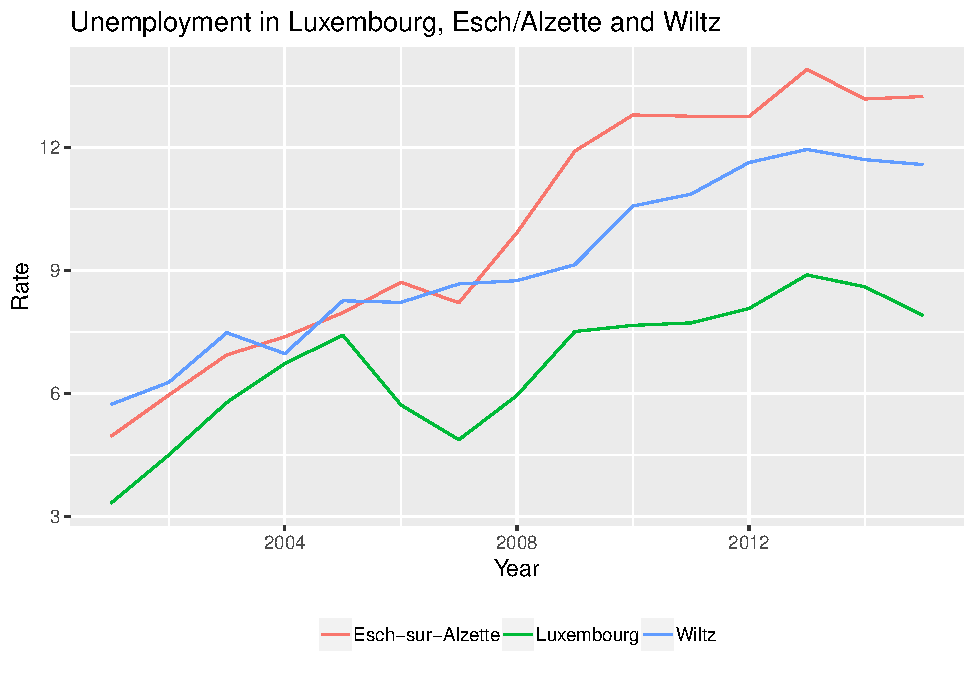
\includegraphics{modern_R_files/figure-latex/unnamed-chunk-323-1.pdf}

The legend title has to be an \texttt{element\_text}
object.\texttt{element\_text} objects are used with \texttt{theme} to
specify how text should be displayed. \texttt{element\_blank()} draws
nothing and assigns no space (not even blank space).

You could modify every feature of the theme like that, but there are
built-in themes that you can use:

\begin{Shaded}
\begin{Highlighting}[]
\NormalTok{unemp_lux_data }\OperatorTok
\StringTok{  }\KeywordTok{filter}\NormalTok{(division }\OperatorTok\StringTok{ }\KeywordTok{c}\NormalTok{(}\StringTok{"Luxembourg"}\NormalTok{, }\StringTok{"Esch-sur-Alzette"}\NormalTok{, }\StringTok{"Wiltz"}\NormalTok{)) }\OperatorTok
\StringTok{  }\KeywordTok{ggplot}\NormalTok{(}\KeywordTok{aes}\NormalTok{(year, unemployment_rate_in_percent, }\DataTypeTok{group =}\NormalTok{ division, }\DataTypeTok{colour =}\NormalTok{ division)) }\OperatorTok{+}
\StringTok{  }\KeywordTok{theme_minimal}\NormalTok{() }\OperatorTok{+}
\StringTok{  }\KeywordTok{theme}\NormalTok{(}\DataTypeTok{legend.position =} \StringTok{"bottom"}\NormalTok{, }\DataTypeTok{legend.title =} \KeywordTok{element_blank}\NormalTok{()) }\OperatorTok{+}
\StringTok{  }\KeywordTok{labs}\NormalTok{(}\DataTypeTok{title =} \StringTok{"Unemployment in Luxembourg, Esch/Alzette and Wiltz"}\NormalTok{, }\DataTypeTok{x =} \StringTok{"Year"}\NormalTok{, }\DataTypeTok{y =} \StringTok{"Rate"}\NormalTok{) }\OperatorTok{+}
\StringTok{  }\KeywordTok{geom_line}\NormalTok{()}
\end{Highlighting}
\end{Shaded}

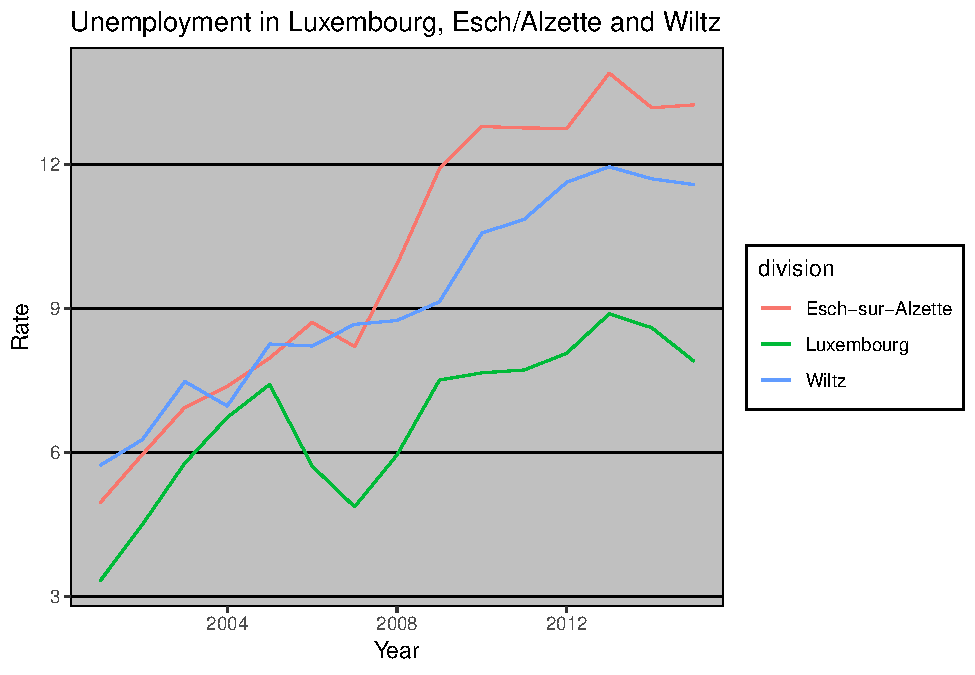
\includegraphics{modern_R_files/figure-latex/unnamed-chunk-324-1.pdf}

For example in the code above, I have used \texttt{theme\_minimal()}
which I like quite a lot. You can also use themes from the
\texttt{ggthemes} package, which even contains a STATA theme, if you
like it:

\begin{Shaded}
\begin{Highlighting}[]
\NormalTok{unemp_lux_data }\OperatorTok
\StringTok{  }\KeywordTok{filter}\NormalTok{(division }\OperatorTok\StringTok{ }\KeywordTok{c}\NormalTok{(}\StringTok{"Luxembourg"}\NormalTok{, }\StringTok{"Esch-sur-Alzette"}\NormalTok{, }\StringTok{"Wiltz"}\NormalTok{)) }\OperatorTok
\StringTok{  }\KeywordTok{ggplot}\NormalTok{(}\KeywordTok{aes}\NormalTok{(year, unemployment_rate_in_percent, }\DataTypeTok{group =}\NormalTok{ division, }\DataTypeTok{colour =}\NormalTok{ division)) }\OperatorTok{+}
\StringTok{  }\KeywordTok{theme_stata}\NormalTok{() }\OperatorTok{+}
\StringTok{  }\KeywordTok{labs}\NormalTok{(}\DataTypeTok{title =} \StringTok{"Unemployment in Luxembourg, Esch/Alzette and Wiltz"}\NormalTok{, }\DataTypeTok{x =} \StringTok{"Year"}\NormalTok{, }\DataTypeTok{y =} \StringTok{"Rate"}\NormalTok{) }\OperatorTok{+}
\StringTok{  }\KeywordTok{geom_line}\NormalTok{()}
\end{Highlighting}
\end{Shaded}

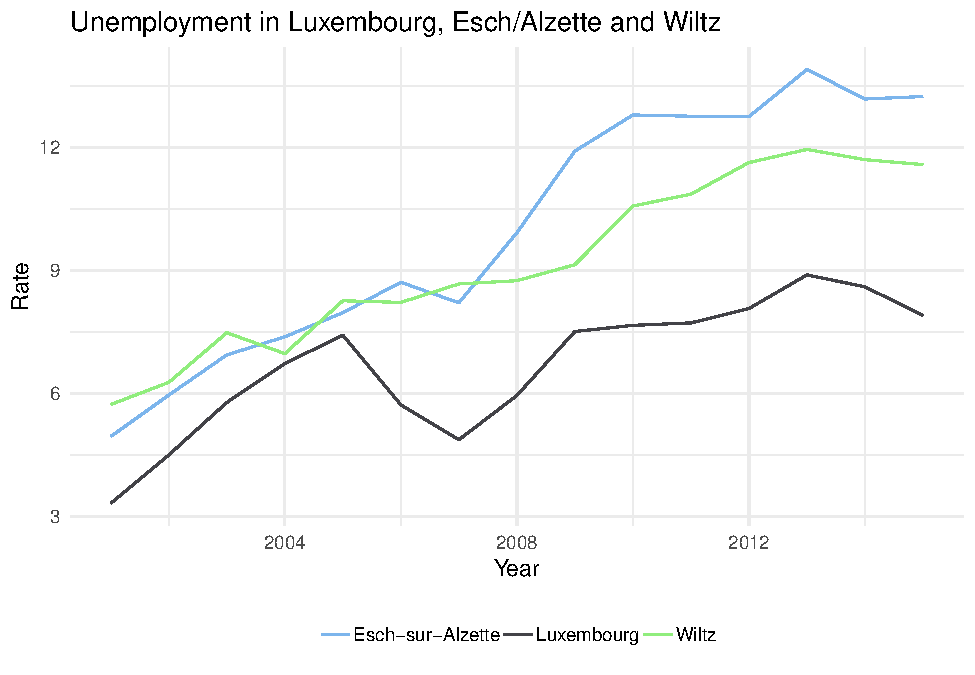
\includegraphics{modern_R_files/figure-latex/unnamed-chunk-325-1.pdf}

As you can see, \texttt{theme\_stata()} has the legend on the bottom by
default, because this is how the legend position is defined within the
theme. However the legend title is still there. Let's remove it:

\begin{Shaded}
\begin{Highlighting}[]
\NormalTok{unemp_lux_data }\OperatorTok
\StringTok{  }\KeywordTok{filter}\NormalTok{(division }\OperatorTok\StringTok{ }\KeywordTok{c}\NormalTok{(}\StringTok{"Luxembourg"}\NormalTok{, }\StringTok{"Esch-sur-Alzette"}\NormalTok{, }\StringTok{"Wiltz"}\NormalTok{)) }\OperatorTok
\StringTok{  }\KeywordTok{ggplot}\NormalTok{(}\KeywordTok{aes}\NormalTok{(year, unemployment_rate_in_percent, }\DataTypeTok{group =}\NormalTok{ division, }\DataTypeTok{colour =}\NormalTok{ division)) }\OperatorTok{+}
\StringTok{  }\KeywordTok{theme_stata}\NormalTok{() }\OperatorTok{+}
\StringTok{  }\KeywordTok{theme}\NormalTok{(}\DataTypeTok{legend.title =} \KeywordTok{element_blank}\NormalTok{()) }\OperatorTok{+}
\StringTok{  }\KeywordTok{labs}\NormalTok{(}\DataTypeTok{title =} \StringTok{"Unemployment in Luxembourg, Esch/Alzette and Wiltz"}\NormalTok{, }\DataTypeTok{x =} \StringTok{"Year"}\NormalTok{, }\DataTypeTok{y =} \StringTok{"Rate"}\NormalTok{) }\OperatorTok{+}
\StringTok{  }\KeywordTok{geom_line}\NormalTok{()}
\end{Highlighting}
\end{Shaded}

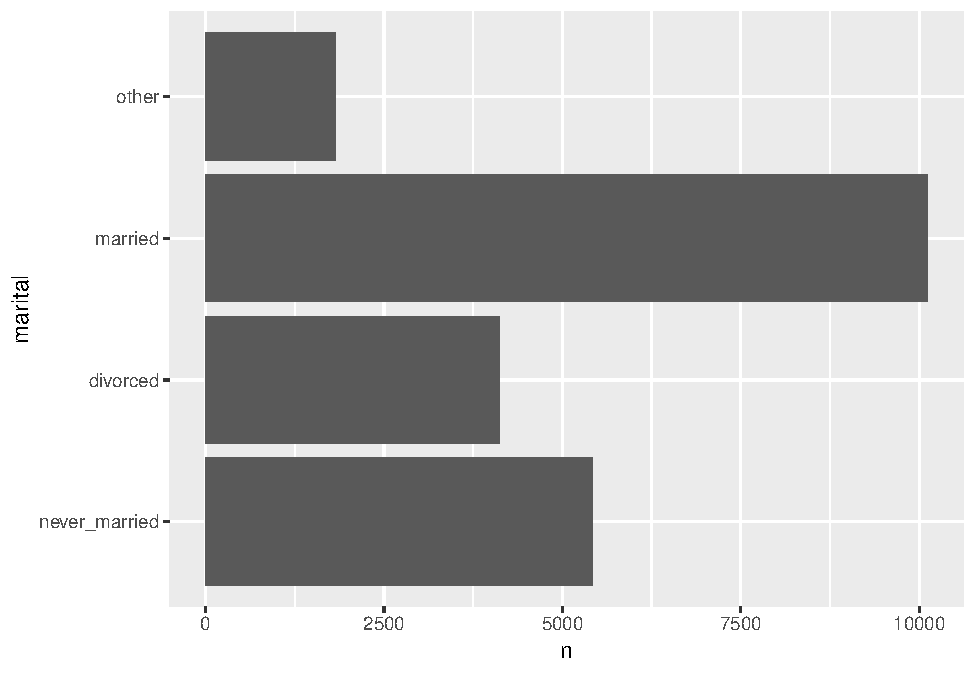
\includegraphics{modern_R_files/figure-latex/unnamed-chunk-326-1.pdf}

\texttt{ggthemes} even features an Excel 2003 theme (don't use it
though):

\begin{Shaded}
\begin{Highlighting}[]
\NormalTok{unemp_lux_data }\OperatorTok
\StringTok{  }\KeywordTok{filter}\NormalTok{(division }\OperatorTok\StringTok{ }\KeywordTok{c}\NormalTok{(}\StringTok{"Luxembourg"}\NormalTok{, }\StringTok{"Esch-sur-Alzette"}\NormalTok{, }\StringTok{"Wiltz"}\NormalTok{)) }\OperatorTok
\StringTok{  }\KeywordTok{ggplot}\NormalTok{(}\KeywordTok{aes}\NormalTok{(year, unemployment_rate_in_percent, }\DataTypeTok{group =}\NormalTok{ division, }\DataTypeTok{colour =}\NormalTok{ division)) }\OperatorTok{+}
\StringTok{  }\KeywordTok{theme_excel}\NormalTok{() }\OperatorTok{+}
\StringTok{  }\KeywordTok{labs}\NormalTok{(}\DataTypeTok{title =} \StringTok{"Unemployment in Luxembourg, Esch/Alzette and Wiltz"}\NormalTok{, }\DataTypeTok{x =} \StringTok{"Year"}\NormalTok{, }\DataTypeTok{y =} \StringTok{"Rate"}\NormalTok{) }\OperatorTok{+}
\StringTok{  }\KeywordTok{geom_line}\NormalTok{()}
\end{Highlighting}
\end{Shaded}

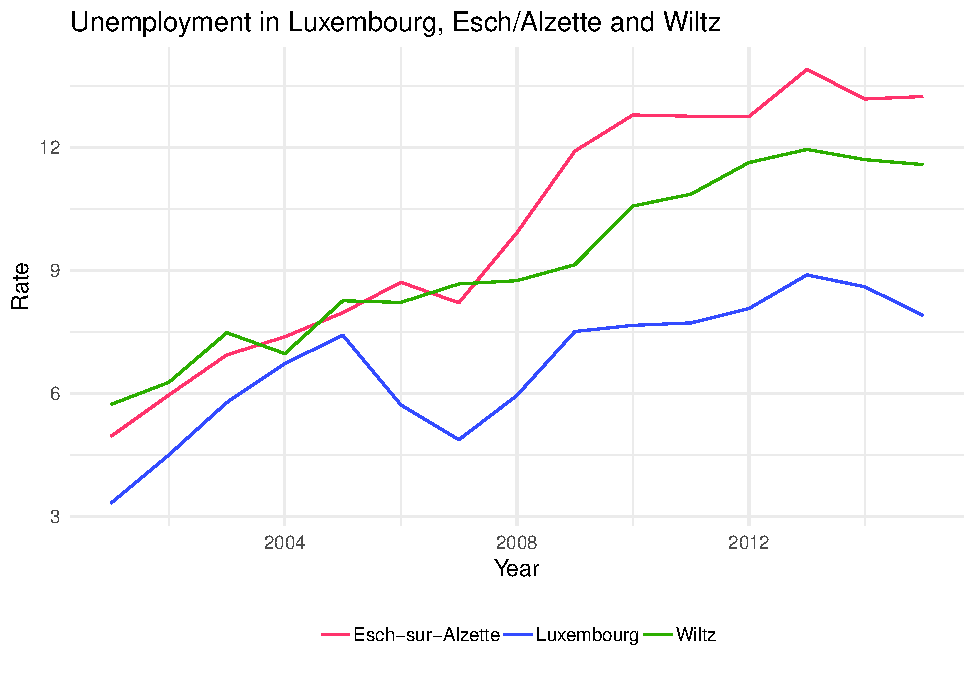
\includegraphics{modern_R_files/figure-latex/unnamed-chunk-327-1.pdf}

\hypertarget{colour-schemes-from-ggthemes}{%
\subsubsection{\texorpdfstring{Colour schemes from
\texttt{ggthemes}}{Colour schemes from ggthemes}}\label{colour-schemes-from-ggthemes}}

You can also change colour schemes, by specifying either
\texttt{scale\_colour\_*} or \texttt{scale\_fill\_*} functions.
\texttt{scale\_colour\_*} functions are used for continuous variables,
while \texttt{scale\_fill\_*} functions for discrete variables (so for
barplots for example). A colour scheme I like is the
\href{https://www.highcharts.com/}{Highcharts} colour scheme.

\begin{Shaded}
\begin{Highlighting}[]
\NormalTok{unemp_lux_data }\OperatorTok
\StringTok{  }\KeywordTok{filter}\NormalTok{(division }\OperatorTok\StringTok{ }\KeywordTok{c}\NormalTok{(}\StringTok{"Luxembourg"}\NormalTok{, }\StringTok{"Esch-sur-Alzette"}\NormalTok{, }\StringTok{"Wiltz"}\NormalTok{)) }\OperatorTok
\StringTok{  }\KeywordTok{ggplot}\NormalTok{(}\KeywordTok{aes}\NormalTok{(year, unemployment_rate_in_percent, }\DataTypeTok{group =}\NormalTok{ division, }\DataTypeTok{colour =}\NormalTok{ division)) }\OperatorTok{+}
\StringTok{  }\KeywordTok{theme_minimal}\NormalTok{() }\OperatorTok{+}
\StringTok{  }\KeywordTok{scale_colour_hc}\NormalTok{() }\OperatorTok{+}
\StringTok{  }\KeywordTok{theme}\NormalTok{(}\DataTypeTok{legend.position =} \StringTok{"bottom"}\NormalTok{, }\DataTypeTok{legend.title =} \KeywordTok{element_blank}\NormalTok{()) }\OperatorTok{+}
\StringTok{  }\KeywordTok{labs}\NormalTok{(}\DataTypeTok{title =} \StringTok{"Unemployment in Luxembourg, Esch/Alzette and Wiltz"}\NormalTok{, }\DataTypeTok{x =} \StringTok{"Year"}\NormalTok{, }\DataTypeTok{y =} \StringTok{"Rate"}\NormalTok{) }\OperatorTok{+}
\StringTok{  }\KeywordTok{geom_line}\NormalTok{()}
\end{Highlighting}
\end{Shaded}

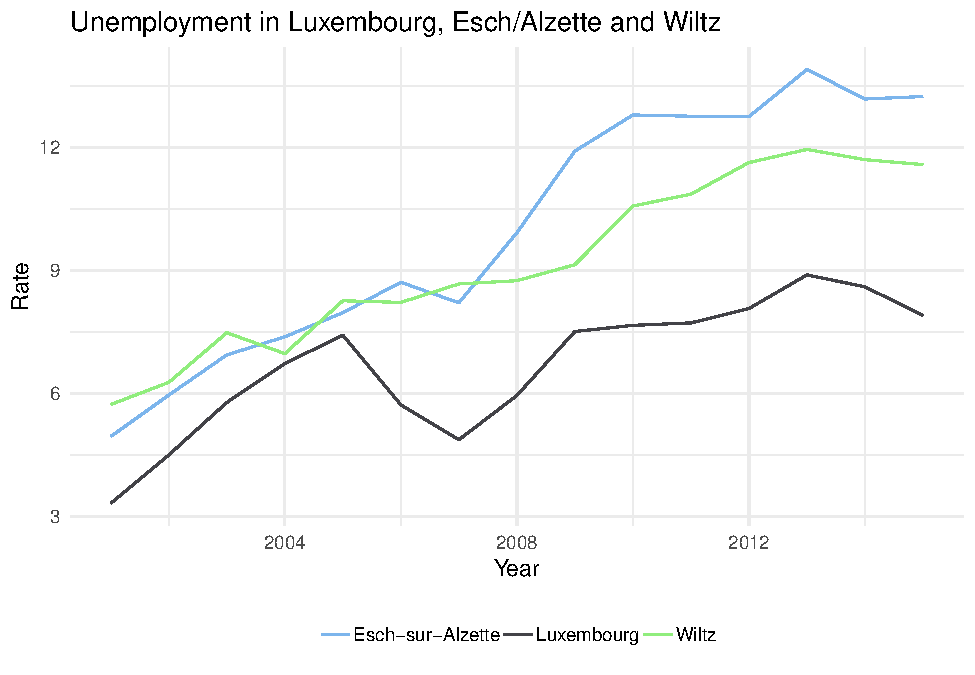
\includegraphics{modern_R_files/figure-latex/unnamed-chunk-328-1.pdf}

An example with a barplot:

\begin{Shaded}
\begin{Highlighting}[]
\KeywordTok{ggplot}\NormalTok{(test_data_long) }\OperatorTok{+}
\StringTok{  }\KeywordTok{facet_wrap}\NormalTok{(}\OperatorTok{~}\NormalTok{id) }\OperatorTok{+}
\StringTok{  }\KeywordTok{geom_bar}\NormalTok{(}\KeywordTok{aes}\NormalTok{(variable, value, }\DataTypeTok{fill =}\NormalTok{ variable), }\DataTypeTok{stat =} \StringTok{"identity"}\NormalTok{) }\OperatorTok{+}
\StringTok{  }\KeywordTok{geom_text}\NormalTok{(}\KeywordTok{aes}\NormalTok{(variable, value }\OperatorTok{+}\StringTok{ }\FloatTok{1.5}\NormalTok{, }\DataTypeTok{label =}\NormalTok{ value)) }\OperatorTok{+}
\StringTok{  }\KeywordTok{theme_minimal}\NormalTok{() }\OperatorTok{+}
\StringTok{  }\KeywordTok{scale_fill_hc}\NormalTok{()}
\end{Highlighting}
\end{Shaded}

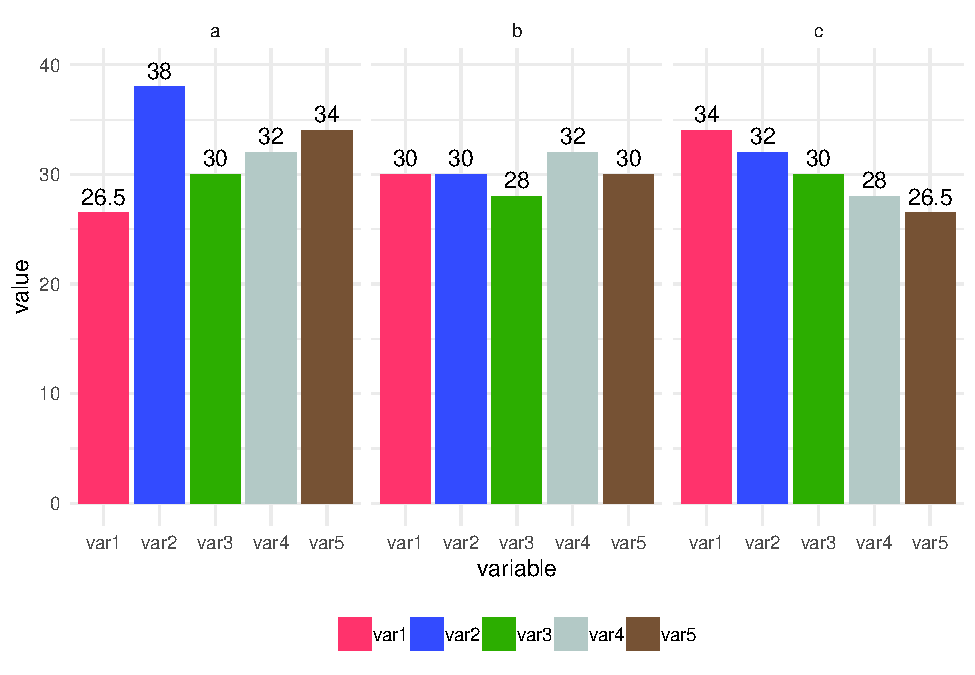
\includegraphics{modern_R_files/figure-latex/unnamed-chunk-329-1.pdf}

\hypertarget{using-your-own-colours}{%
\subsubsection{Using your own colours}\label{using-your-own-colours}}

To use your own colours you can use \texttt{scale\_colour\_manual()} and
\texttt{scale\_fill\_manual()} and specify the html codes of the colours
you want to use.

\begin{Shaded}
\begin{Highlighting}[]
\NormalTok{unemp_lux_data }\OperatorTok
\StringTok{  }\KeywordTok{filter}\NormalTok{(division }\OperatorTok\StringTok{ }\KeywordTok{c}\NormalTok{(}\StringTok{"Luxembourg"}\NormalTok{, }\StringTok{"Esch-sur-Alzette"}\NormalTok{, }\StringTok{"Wiltz"}\NormalTok{)) }\OperatorTok
\StringTok{  }\KeywordTok{ggplot}\NormalTok{(}\KeywordTok{aes}\NormalTok{(year, unemployment_rate_in_percent, }\DataTypeTok{group =}\NormalTok{ division, }\DataTypeTok{colour =}\NormalTok{ division)) }\OperatorTok{+}
\StringTok{  }\KeywordTok{theme_minimal}\NormalTok{() }\OperatorTok{+}
\StringTok{  }\KeywordTok{scale_colour_manual}\NormalTok{(}\DataTypeTok{values =} \KeywordTok{c}\NormalTok{(}\StringTok{"#FF336C"}\NormalTok{, }\StringTok{"#334BFF"}\NormalTok{, }\StringTok{"#2CAE00"}\NormalTok{)) }\OperatorTok{+}
\StringTok{  }\KeywordTok{theme}\NormalTok{(}\DataTypeTok{legend.position =} \StringTok{"bottom"}\NormalTok{, }\DataTypeTok{legend.title =} \KeywordTok{element_blank}\NormalTok{()) }\OperatorTok{+}
\StringTok{  }\KeywordTok{labs}\NormalTok{(}\DataTypeTok{title =} \StringTok{"Unemployment in Luxembourg, Esch/Alzette and Wiltz"}\NormalTok{, }\DataTypeTok{x =} \StringTok{"Year"}\NormalTok{, }\DataTypeTok{y =} \StringTok{"Rate"}\NormalTok{) }\OperatorTok{+}
\StringTok{  }\KeywordTok{geom_line}\NormalTok{()}
\end{Highlighting}
\end{Shaded}

\includegraphics{modern_R_files/figure-latex/unnamed-chunk-330-1.pdf}

To get html codes of colours you can use
\href{http://htmlcolorcodes.com/color-picker/}{this online tool}. There
is also a very nice package, called \texttt{colourpicker} that allows
you to pick colours from with RStudio. Also, you do not even need to
load it to use it, since it comes with an Addin:

\includegraphics{pics/rstudio_colourpicker.gif}

For a barplot you would do the same:

\begin{Shaded}
\begin{Highlighting}[]
\KeywordTok{ggplot}\NormalTok{(test_data_long) }\OperatorTok{+}
\StringTok{  }\KeywordTok{facet_wrap}\NormalTok{(}\OperatorTok{~}\NormalTok{id) }\OperatorTok{+}
\StringTok{  }\KeywordTok{geom_bar}\NormalTok{(}\KeywordTok{aes}\NormalTok{(variable, value, }\DataTypeTok{fill =}\NormalTok{ variable), }\DataTypeTok{stat =} \StringTok{"identity"}\NormalTok{) }\OperatorTok{+}
\StringTok{  }\KeywordTok{geom_text}\NormalTok{(}\KeywordTok{aes}\NormalTok{(variable, value }\OperatorTok{+}\StringTok{ }\FloatTok{1.5}\NormalTok{, }\DataTypeTok{label =}\NormalTok{ value)) }\OperatorTok{+}
\StringTok{  }\KeywordTok{theme_minimal}\NormalTok{() }\OperatorTok{+}
\StringTok{  }\KeywordTok{theme}\NormalTok{(}\DataTypeTok{legend.position =} \StringTok{"bottom"}\NormalTok{, }\DataTypeTok{legend.title =} \KeywordTok{element_blank}\NormalTok{()) }\OperatorTok{+}
\StringTok{  }\KeywordTok{scale_fill_manual}\NormalTok{(}\DataTypeTok{values =} \KeywordTok{c}\NormalTok{(}\StringTok{"#FF336C"}\NormalTok{, }\StringTok{"#334BFF"}\NormalTok{, }\StringTok{"#2CAE00"}\NormalTok{, }\StringTok{"#B3C9C6"}\NormalTok{, }\StringTok{"#765234"}\NormalTok{))}
\end{Highlighting}
\end{Shaded}

\includegraphics{modern_R_files/figure-latex/unnamed-chunk-332-1.pdf}

\hypertarget{saving-plots-on-disk}{%
\subsubsection{Saving plots on disk}\label{saving-plots-on-disk}}

There are two ways to save plots on disk; one through the \emph{Plots}
in RStudio and another using the \texttt{ggsave()} function. Using
RStudio, navigate to the \emph{Plots} pane and click on \emph{Export}.
You can then choose where to save the plot and other various options:

\begin{Shaded}
\begin{Highlighting}[]
\NormalTok{knitr}\OperatorTok{::}\KeywordTok{include_graphics}\NormalTok{(}\StringTok{"pics/rstudio_save_plots.gif"}\NormalTok{)}
\end{Highlighting}
\end{Shaded}

\includegraphics{pics/rstudio_save_plots.gif}

This is fine if you only generate one or two plots but if you generate a
large number of them, it is less tedious to use the \texttt{ggsave()}
function:

\begin{Shaded}
\begin{Highlighting}[]
\NormalTok{my_plot1 =}\StringTok{ }\KeywordTok{ggplot}\NormalTok{(my_data) }\OperatorTok{+}
\StringTok{  }\KeywordTok{geom_bar}\NormalTok{(}\KeywordTok{aes}\NormalTok{(variable))}

\KeywordTok{ggsave}\NormalTok{(}\StringTok{"path/you/want/to/save/the/plot/to/my_plot1.pdf"}\NormalTok{, my_plot1)}
\end{Highlighting}
\end{Shaded}

There are other options that you can specify such as the width and
height, resolution, units, etc\ldots{}

\hypertarget{exercises-3}{%
\subsection{Exercises}\label{exercises-3}}

\hypertarget{exercise-1-3}{%
\subsubsection*{Exercise 1}\label{exercise-1-3}}
\addcontentsline{toc}{subsubsection}{Exercise 1}

This exercise will force you to look for \texttt{ggplot2} functions that
you don't know yet. But it's a good exercise, so my advice is to try to
do it, even if takes you a long time to find the right functions.

Load the \texttt{Bwages} dataset from the \texttt{Ecdat} package. Your
first task is to create a new variable, \texttt{educ\_level}, which is a
factor variable that equals:

\begin{itemize}
\tightlist
\item
  ``Primary school'' if \texttt{educ\ ==\ 1}
\item
  ``High school'' if \texttt{educ\ ==\ 2}
\item
  ``Some university'' if \texttt{educ\ ==\ 3}
\item
  ``Master's degree'' if \texttt{educ\ ==\ 4}
\item
  ``Doctoral degree'' if \texttt{educ\ ==\ 5}
\end{itemize}

Use \texttt{case\_when()} for this.

Then, plot a scatter plot of wages on experience, by education level.
Add a theme that you like, and remove the title of the legend.

The scatter plot is not very useful, because you cannot make anything
out. Instead, use another geom that shows you a non-parametric fit with
confidence bands. You do not need to estimate a model or anything like
that, you just need to find the right geom.

\hypertarget{statistical-models}{%
\section{Statistical models}\label{statistical-models}}

In this chapter, we will not learn about all the models out there that
you may or may not need. Instead, I will show you how can use what you
have learned until now and how you can apply these concepts to modeling.
Also, as you read in the beginning of the book, R has many many
packages. So the model you need is most probably already implemented in
some package and you will very likely not need to write your own from
scratch.

In the first section, I will discuss the terminology used in this book.
Then I will discuss linear regression; showing how linear regression
works illsutrates very well how other models work too, without loss of
generality. Then I will introduce the concepte of hyper-parameters with
ridge regression. This chapter will then finish with an introduction to
cross-validation as a way to tune the hyper-parameters of models that
features them.

\hypertarget{terminology}{%
\subsection{Terminology}\label{terminology}}

Before continuing discussing about statistical models and model fitting
it is worthwhile to discuss terminology a little bit. Depending on your
background, you might call an explanatory variable a feature or the
dependent variable the target. These are the same objects. The matrix of
features is usually called a design matrix, and the what statisticians
call the intercept in a linear regression machine learning engineers
call the bias. Calling the intercept the bias is unfortunate, as bias
also has a very different meaning; bias is also what we call the error
in a model that may cause \emph{biased} estimates. To finish up, the
estimated parameters of the model may be called coefficients or weights.
Here again, I don't like the using \emph{weight} as weight as a very
different meaning in statistics. So, in the remainder of this chapter,
and book, I will use the terminology from the statistical litterature,
using dependent and explanatory variables (\texttt{y} and \texttt{x}),
and calling the estimated parameters coefficients and the
intercept\ldots{} well the intercept (the \(\beta\)s of the model).
However, I will talk of \emph{training} a model, instead of
\emph{estimating} a model.

\hypertarget{fitting-a-model-to-data}{%
\subsection{Fitting a model to data}\label{fitting-a-model-to-data}}

Suppose you have a variable \texttt{y} that you wish to explain using a
set of other variables \texttt{x1}, \texttt{x2}, \texttt{x3}, etc. Let's
take a look at the \texttt{Housing} dataset from the \texttt{Ecdat}
package:

\begin{Shaded}
\begin{Highlighting}[]
\KeywordTok{library}\NormalTok{(Ecdat)}

\KeywordTok{data}\NormalTok{(Housing)}
\end{Highlighting}
\end{Shaded}

You can read a description of the dataset by running:

\begin{Shaded}
\begin{Highlighting}[]
\NormalTok{?Housing}
\end{Highlighting}
\end{Shaded}

\begin{verbatim}
Housing                 package:Ecdat                  R Documentation

Sales Prices of Houses in the City of Windsor

Description:

     a cross-section from 1987

     _number of observations_ : 546

     _observation_ : goods

     _country_ : Canada

Usage:

     data(Housing)

Format:

     A dataframe containing :

     price: sale price of a house

     lotsize: the lot size of a property in square feet

     bedrooms: number of bedrooms

     bathrms: number of full bathrooms

     stories: number of stories excluding basement

     driveway: does the house has a driveway ?

     recroom: does the house has a recreational room ?

     fullbase: does the house has a full finished basement ?

     gashw: does the house uses gas for hot water heating ?

     airco: does the house has central air conditioning ?

     garagepl: number of garage places

     prefarea: is the house located in the preferred neighbourhood of the city ?

Source:

     Anglin, P.M.  and R.  Gencay (1996) “Semiparametric estimation of
     a hedonic price function”, _Journal of Applied Econometrics_,
     *11(6)*, 633-648.

References:

     Verbeek, Marno (2004) _A Guide to Modern Econometrics_, John Wiley
     and Sons, chapter 3.

     Journal of Applied Econometrics data archive : <URL:
     http://qed.econ.queensu.ca/jae/>.

See Also:

     ‘Index.Source’, ‘Index.Economics’, ‘Index.Econometrics’,
     ‘Index.Observations’
\end{verbatim}

or by looking for \texttt{Housing} in the help pane of RStudio. Usually,
you would take a look a the data before doing any modeling:

\begin{Shaded}
\begin{Highlighting}[]
\KeywordTok{glimpse}\NormalTok{(Housing)}
\end{Highlighting}
\end{Shaded}

\begin{verbatim}
## Observations: 546
## Variables: 12
## $ price    <dbl> 42000, 38500, 49500, 60500, 61000, 66000, 66000, 6900...
## $ lotsize  <dbl> 5850, 4000, 3060, 6650, 6360, 4160, 3880, 4160, 4800,...
## $ bedrooms <dbl> 3, 2, 3, 3, 2, 3, 3, 3, 3, 3, 3, 2, 3, 3, 2, 2, 3, 4,...
## $ bathrms  <dbl> 1, 1, 1, 1, 1, 1, 2, 1, 1, 2, 2, 1, 1, 1, 1, 1, 1, 1,...
## $ stories  <dbl> 2, 1, 1, 2, 1, 1, 2, 3, 1, 4, 1, 1, 2, 1, 1, 1, 2, 3,...
## $ driveway <fct> yes, yes, yes, yes, yes, yes, yes, yes, yes, yes, yes...
## $ recroom  <fct> no, no, no, yes, no, yes, no, no, yes, yes, no, no, n...
## $ fullbase <fct> yes, no, no, no, no, yes, yes, no, yes, no, yes, no, ...
## $ gashw    <fct> no, no, no, no, no, no, no, no, no, no, no, no, no, n...
## $ airco    <fct> no, no, no, no, no, yes, no, no, no, yes, yes, no, no...
## $ garagepl <dbl> 1, 0, 0, 0, 0, 0, 2, 0, 0, 1, 3, 0, 0, 0, 0, 0, 1, 0,...
## $ prefarea <fct> no, no, no, no, no, no, no, no, no, no, no, no, no, n...
\end{verbatim}

Housing prices depend on a set of variables such as the number of
bedrooms, the area it is located and so on. If you believe that housing
prices depend linearly on a set of explanatory variables, you will want
to estimate a linear model. To estimate a \emph{linear model}, you will
need to use the built-in \texttt{lm()} function:

\begin{Shaded}
\begin{Highlighting}[]
\NormalTok{model1 <-}\StringTok{ }\KeywordTok{lm}\NormalTok{(price }\OperatorTok{~}\StringTok{ }\NormalTok{lotsize }\OperatorTok{+}\StringTok{ }\NormalTok{bedrooms, }\DataTypeTok{data =}\NormalTok{ Housing)}
\end{Highlighting}
\end{Shaded}

\texttt{lm()} takes a formula as an argument, which defines the model
you want to estimate. In this case, I ran the following regression:

\[
\text{price} = \beta_0 + \beta_1 * \text{lotsize} + \beta_2 * \text{bedrooms} + \varepsilon
\]

where \(\beta_0, \beta_1\) and \(\beta_2\) are three parameters to
estimate. To take a look at the results, you can use the
\texttt{summary()} method (not to be confused with
\texttt{dplyr::summarise()}:

\begin{Shaded}
\begin{Highlighting}[]
\KeywordTok{summary}\NormalTok{(model1)}
\end{Highlighting}
\end{Shaded}

\begin{verbatim}
## 
## Call:
## lm(formula = price ~ lotsize + bedrooms, data = Housing)
## 
## Residuals:
##    Min     1Q Median     3Q    Max 
## -65665 -12498  -2075   8970  97205 
## 
## Coefficients:
##              Estimate Std. Error t value Pr(>|t|)    
## (Intercept) 5.613e+03  4.103e+03   1.368    0.172    
## lotsize     6.053e+00  4.243e-01  14.265  < 2e-16 ***
## bedrooms    1.057e+04  1.248e+03   8.470 2.31e-16 ***
## ---
## Signif. codes:  0 '***' 0.001 '**' 0.01 '*' 0.05 '.' 0.1 ' ' 1
## 
## Residual standard error: 21230 on 543 degrees of freedom
## Multiple R-squared:  0.3703, Adjusted R-squared:  0.3679 
## F-statistic: 159.6 on 2 and 543 DF,  p-value: < 2.2e-16
\end{verbatim}

if you wish to remove the intercept (\(alpha\)) from your model, you can
do so with \texttt{-1}:

\begin{Shaded}
\begin{Highlighting}[]
\NormalTok{model2 <-}\StringTok{ }\KeywordTok{lm}\NormalTok{(price }\OperatorTok{~}\StringTok{ }\DecValTok{-1} \OperatorTok{+}\StringTok{ }\NormalTok{lotsize }\OperatorTok{+}\StringTok{ }\NormalTok{bedrooms, }\DataTypeTok{data =}\NormalTok{ Housing)}

\KeywordTok{summary}\NormalTok{(model2)}
\end{Highlighting}
\end{Shaded}

\begin{verbatim}
## 
## Call:
## lm(formula = price ~ -1 + lotsize + bedrooms, data = Housing)
## 
## Residuals:
##    Min     1Q Median     3Q    Max 
## -67229 -12342  -1333   9627  95509 
## 
## Coefficients:
##           Estimate Std. Error t value Pr(>|t|)    
## lotsize      6.283      0.390   16.11   <2e-16 ***
## bedrooms 11968.362    713.194   16.78   <2e-16 ***
## ---
## Signif. codes:  0 '***' 0.001 '**' 0.01 '*' 0.05 '.' 0.1 ' ' 1
## 
## Residual standard error: 21250 on 544 degrees of freedom
## Multiple R-squared:  0.916,  Adjusted R-squared:  0.9157 
## F-statistic:  2965 on 2 and 544 DF,  p-value: < 2.2e-16
\end{verbatim}

or if you want to use all the columns inside \texttt{Housing}:

\begin{Shaded}
\begin{Highlighting}[]
\NormalTok{model3 <-}\StringTok{ }\KeywordTok{lm}\NormalTok{(price }\OperatorTok{~}\StringTok{ }\NormalTok{., }\DataTypeTok{data =}\NormalTok{ Housing)}

\KeywordTok{summary}\NormalTok{(model3)}
\end{Highlighting}
\end{Shaded}

\begin{verbatim}
## 
## Call:
## lm(formula = price ~ ., data = Housing)
## 
## Residuals:
##    Min     1Q Median     3Q    Max 
## -41389  -9307   -591   7353  74875 
## 
## Coefficients:
##               Estimate Std. Error t value Pr(>|t|)    
## (Intercept) -4038.3504  3409.4713  -1.184 0.236762    
## lotsize         3.5463     0.3503  10.124  < 2e-16 ***
## bedrooms     1832.0035  1047.0002   1.750 0.080733 .  
## bathrms     14335.5585  1489.9209   9.622  < 2e-16 ***
## stories      6556.9457   925.2899   7.086 4.37e-12 ***
## drivewayyes  6687.7789  2045.2458   3.270 0.001145 ** 
## recroomyes   4511.2838  1899.9577   2.374 0.017929 *  
## fullbaseyes  5452.3855  1588.0239   3.433 0.000642 ***
## gashwyes    12831.4063  3217.5971   3.988 7.60e-05 ***
## aircoyes    12632.8904  1555.0211   8.124 3.15e-15 ***
## garagepl     4244.8290   840.5442   5.050 6.07e-07 ***
## prefareayes  9369.5132  1669.0907   5.614 3.19e-08 ***
## ---
## Signif. codes:  0 '***' 0.001 '**' 0.01 '*' 0.05 '.' 0.1 ' ' 1
## 
## Residual standard error: 15420 on 534 degrees of freedom
## Multiple R-squared:  0.6731, Adjusted R-squared:  0.6664 
## F-statistic: 99.97 on 11 and 534 DF,  p-value: < 2.2e-16
\end{verbatim}

You can access different elements of \texttt{model3} (for example) with
\texttt{\$}, because the result of \texttt{lm()} is a list:

\begin{Shaded}
\begin{Highlighting}[]
\KeywordTok{print}\NormalTok{(model3}\OperatorTok{$}\NormalTok{coefficients)}
\end{Highlighting}
\end{Shaded}

\begin{verbatim}
##  (Intercept)      lotsize     bedrooms      bathrms      stories 
## -4038.350425     3.546303  1832.003466 14335.558468  6556.945711 
##  drivewayyes   recroomyes  fullbaseyes     gashwyes     aircoyes 
##  6687.778890  4511.283826  5452.385539 12831.406266 12632.890405 
##     garagepl  prefareayes 
##  4244.829004  9369.513239
\end{verbatim}

but I prefer to use the \texttt{\{broom\}} package, and more
specifically the \texttt{tidy()} function, which converts
\texttt{model3} into a neat \texttt{data.frame}:

\begin{Shaded}
\begin{Highlighting}[]
\NormalTok{results3 <-}\StringTok{ }\NormalTok{broom}\OperatorTok{::}\KeywordTok{tidy}\NormalTok{(model3)}

\KeywordTok{glimpse}\NormalTok{(results3)}
\end{Highlighting}
\end{Shaded}

\begin{verbatim}
## Observations: 12
## Variables: 5
## $ term      <chr> "(Intercept)", "lotsize", "bedrooms", "bathrms", "st...
## $ estimate  <dbl> -4038.350425, 3.546303, 1832.003466, 14335.558468, 6...
## $ std.error <dbl> 3409.4713, 0.3503, 1047.0002, 1489.9209, 925.2899, 2...
## $ statistic <dbl> -1.184451, 10.123618, 1.749764, 9.621691, 7.086369, ...
## $ p.value   <dbl> 2.367616e-01, 3.732442e-22, 8.073341e-02, 2.570369e-...
\end{verbatim}

I explicitely write \texttt{broom::tidy()} because \texttt{tidy()} is a
popular function name. For instance, it is also a function from the
\texttt{\{yardstick\}} package, which does not do the same thing at all.
Since I will also be using \texttt{\{yardstick\}} I prefer explicitely
writing \texttt{broom::tidy()} to avoid conflicts.

Using \texttt{broom::tidy()} is useful, because you can then work on the
results easily, for example if you wish to only keep results that are
significant at the 5\% level:

\begin{Shaded}
\begin{Highlighting}[]
\NormalTok{results3 }\OperatorTok
\StringTok{  }\KeywordTok{filter}\NormalTok{(p.value }\OperatorTok{<}\StringTok{ }\FloatTok{0.05}\NormalTok{)}
\end{Highlighting}
\end{Shaded}

\begin{verbatim}
## # A tibble: 10 x 5
##    term        estimate std.error statistic  p.value
##    <chr>          <dbl>     <dbl>     <dbl>    <dbl>
##  1 lotsize         3.55     0.350     10.1  3.73e-22
##  2 bathrms     14336.    1490.         9.62 2.57e-20
##  3 stories      6557.     925.         7.09 4.37e-12
##  4 drivewayyes  6688.    2045.         3.27 1.15e- 3
##  5 recroomyes   4511.    1900.         2.37 1.79e- 2
##  6 fullbaseyes  5452.    1588.         3.43 6.42e- 4
##  7 gashwyes    12831.    3218.         3.99 7.60e- 5
##  8 aircoyes    12633.    1555.         8.12 3.15e-15
##  9 garagepl     4245.     841.         5.05 6.07e- 7
## 10 prefareayes  9370.    1669.         5.61 3.19e- 8
\end{verbatim}

You can even add new columns, such as the confidence intervals:

\begin{Shaded}
\begin{Highlighting}[]
\NormalTok{results3 <-}\StringTok{ }\NormalTok{broom}\OperatorTok{::}\KeywordTok{tidy}\NormalTok{(model3, }\DataTypeTok{conf.int =} \OtherTok{TRUE}\NormalTok{, }\DataTypeTok{conf.level =} \FloatTok{0.95}\NormalTok{)}

\KeywordTok{print}\NormalTok{(results3)}
\end{Highlighting}
\end{Shaded}

\begin{verbatim}
## # A tibble: 12 x 7
##    term         estimate std.error statistic  p.value  conf.low conf.high
##    <chr>           <dbl>     <dbl>     <dbl>    <dbl>     <dbl>     <dbl>
##  1 (Intercept)  -4038.    3409.        -1.18 2.37e- 1 -10736.     2659.  
##  2 lotsize          3.55     0.350     10.1  3.73e-22      2.86      4.23
##  3 bedrooms      1832.    1047.         1.75 8.07e- 2   -225.     3889.  
##  4 bathrms      14336.    1490.         9.62 2.57e-20  11409.    17262.  
##  5 stories       6557.     925.         7.09 4.37e-12   4739.     8375.  
##  6 drivewayyes   6688.    2045.         3.27 1.15e- 3   2670.    10705.  
##  7 recroomyes    4511.    1900.         2.37 1.79e- 2    779.     8244.  
##  8 fullbaseyes   5452.    1588.         3.43 6.42e- 4   2333.     8572.  
##  9 gashwyes     12831.    3218.         3.99 7.60e- 5   6511.    19152.  
## 10 aircoyes     12633.    1555.         8.12 3.15e-15   9578.    15688.  
## 11 garagepl      4245.     841.         5.05 6.07e- 7   2594.     5896.  
## 12 prefareayes   9370.    1669.         5.61 3.19e- 8   6091.    12648.
\end{verbatim}

Going back to model estimation, you can of course use \texttt{lm()} in a
pipe workflow:

\begin{Shaded}
\begin{Highlighting}[]
\NormalTok{Housing }\OperatorTok
\StringTok{  }\KeywordTok{select}\NormalTok{(}\OperatorTok{-}\NormalTok{driveway, }\OperatorTok{-}\NormalTok{stories) }\OperatorTok
\StringTok{  }\KeywordTok{lm}\NormalTok{(price }\OperatorTok{~}\StringTok{ }\NormalTok{., }\DataTypeTok{data =}\NormalTok{ .) }\OperatorTok
\StringTok{  }\NormalTok{broom}\OperatorTok{::}\KeywordTok{tidy}\NormalTok{()}
\end{Highlighting}
\end{Shaded}

\begin{verbatim}
## # A tibble: 10 x 5
##    term        estimate std.error statistic  p.value
##    <chr>          <dbl>     <dbl>     <dbl>    <dbl>
##  1 (Intercept)  3025.    3263.        0.927 3.54e- 1
##  2 lotsize         3.67     0.363    10.1   4.52e-22
##  3 bedrooms     4140.    1036.        3.99  7.38e- 5
##  4 bathrms     16443.    1546.       10.6   4.29e-24
##  5 recroomyes   5660.    2010.        2.82  5.05e- 3
##  6 fullbaseyes  2241.    1618.        1.38  1.67e- 1
##  7 gashwyes    13568.    3411.        3.98  7.93e- 5
##  8 aircoyes    15578.    1597.        9.75  8.53e-21
##  9 garagepl     4232.     883.        4.79  2.12e- 6
## 10 prefareayes 10729.    1753.        6.12  1.81e- 9
\end{verbatim}

The first \texttt{.} in the \texttt{lm()} function is used to indicate
that we wish to use all the data from \texttt{Housing} (minus
\texttt{driveway} and \texttt{stories} which I removed using
\texttt{select()} and the \texttt{-} sign), and the second \texttt{.} is
used to \emph{place} the result from the two \texttt{dplyr} instructions
that preceded is to be placed there. The picture below should help you
understand:

\begin{Shaded}
\begin{Highlighting}[]
\NormalTok{knitr}\OperatorTok{::}\KeywordTok{include_graphics}\NormalTok{(}\StringTok{"pics/pipe_to_second_position.png"}\NormalTok{)}
\end{Highlighting}
\end{Shaded}

\includegraphics[width=8in]{pics/pipe_to_second_position}

You have to specify this, because by default, when using
\texttt{\%\textgreater{}\%} the left hand side argument gets passed as
the first argument of the function on the right hand side.

\hypertarget{diagnostics}{%
\subsection{Diagnostics}\label{diagnostics}}

Diagnostics are useful metrics to assess model fit. You can read some of
these diagnostics, such as the \(R^2\) at the bottom of the summary
(when running \texttt{summary(my\_model)}), but if you want to do more
than simply reading these diagnostics from RStudio, you can put those in
a \texttt{data.frame} too, using \texttt{broom::glance()}:

\begin{Shaded}
\begin{Highlighting}[]
\KeywordTok{glance}\NormalTok{(model3)}
\end{Highlighting}
\end{Shaded}

\begin{verbatim}
## # A tibble: 1 x 11
##   r.squared adj.r.squared  sigma statistic   p.value    df logLik    AIC
## *     <dbl>         <dbl>  <dbl>     <dbl>     <dbl> <int>  <dbl>  <dbl>
## 1     0.673         0.666 15423.     100.0 6.18e-122    12 -6034. 12094.
## # ... with 3 more variables: BIC <dbl>, deviance <dbl>, df.residual <int>
\end{verbatim}

You can also plot the usual diagnostics plots using
\texttt{ggfortify::autoplot()} which uses the \texttt{ggplot2} package
under the hood:

\begin{Shaded}
\begin{Highlighting}[]
\KeywordTok{library}\NormalTok{(ggfortify)}

\KeywordTok{autoplot}\NormalTok{(model3, }\DataTypeTok{which =} \DecValTok{1}\OperatorTok{:}\DecValTok{6}\NormalTok{) }\OperatorTok{+}\StringTok{ }\KeywordTok{theme_minimal}\NormalTok{()}
\end{Highlighting}
\end{Shaded}

\includegraphics{modern_R_files/figure-latex/unnamed-chunk-353-1.pdf}

\texttt{which=1:6} is an additional option that shows you all the
diagnostics plot. If you omit this option, you will only get 4 of them.

You can also get the residuals of the regression in two ways; either you
grab them directly from the model fit:

\begin{Shaded}
\begin{Highlighting}[]
\NormalTok{resi3 <-}\StringTok{ }\KeywordTok{residuals}\NormalTok{(model3)}
\end{Highlighting}
\end{Shaded}

or you can augment the original data with a residuals column, using
\texttt{broom::augment()}:

\begin{Shaded}
\begin{Highlighting}[]
\NormalTok{housing_aug <-}\StringTok{ }\KeywordTok{augment}\NormalTok{(model3)}
\end{Highlighting}
\end{Shaded}

Let's take a look at \texttt{housing\_aug}:

\begin{Shaded}
\begin{Highlighting}[]
\KeywordTok{glimpse}\NormalTok{(housing_aug)}
\end{Highlighting}
\end{Shaded}

\begin{verbatim}
## Observations: 546
## Variables: 19
## $ price      <dbl> 42000, 38500, 49500, 60500, 61000, 66000, 66000, 69...
## $ lotsize    <dbl> 5850, 4000, 3060, 6650, 6360, 4160, 3880, 4160, 480...
## $ bedrooms   <dbl> 3, 2, 3, 3, 2, 3, 3, 3, 3, 3, 3, 2, 3, 3, 2, 2, 3, ...
## $ bathrms    <dbl> 1, 1, 1, 1, 1, 1, 2, 1, 1, 2, 2, 1, 1, 1, 1, 1, 1, ...
## $ stories    <dbl> 2, 1, 1, 2, 1, 1, 2, 3, 1, 4, 1, 1, 2, 1, 1, 1, 2, ...
## $ driveway   <fct> yes, yes, yes, yes, yes, yes, yes, yes, yes, yes, y...
## $ recroom    <fct> no, no, no, yes, no, yes, no, no, yes, yes, no, no,...
## $ fullbase   <fct> yes, no, no, no, no, yes, yes, no, yes, no, yes, no...
## $ gashw      <fct> no, no, no, no, no, no, no, no, no, no, no, no, no,...
## $ airco      <fct> no, no, no, no, no, yes, no, no, no, yes, yes, no, ...
## $ garagepl   <dbl> 1, 0, 0, 0, 0, 0, 2, 0, 0, 1, 3, 0, 0, 0, 0, 0, 1, ...
## $ prefarea   <fct> no, no, no, no, no, no, no, no, no, no, no, no, no,...
## $ .fitted    <dbl> 66037.98, 41391.15, 39889.63, 63689.09, 49760.43, 6...
## $ .se.fit    <dbl> 1790.507, 1406.500, 1534.102, 2262.056, 1567.689, 2...
## $ .resid     <dbl> -24037.9757, -2891.1515, 9610.3699, -3189.0873, 112...
## $ .hat       <dbl> 0.013477335, 0.008316321, 0.009893730, 0.021510891,...
## $ .sigma     <dbl> 15402.01, 15437.14, 15431.98, 15437.02, 15429.89, 1...
## $ .cooksd    <dbl> 2.803214e-03, 2.476265e-05, 3.265481e-04, 8.004787e...
## $ .std.resid <dbl> -1.56917096, -0.18823924, 0.62621736, -0.20903274, ...
\end{verbatim}

A few columns have been added to the original data, among them
\texttt{.resid} which contains the residuals. Let's plot them:

\begin{Shaded}
\begin{Highlighting}[]
\KeywordTok{ggplot}\NormalTok{(housing_aug) }\OperatorTok{+}
\StringTok{  }\KeywordTok{geom_density}\NormalTok{(}\KeywordTok{aes}\NormalTok{(.resid))}
\end{Highlighting}
\end{Shaded}

\includegraphics{modern_R_files/figure-latex/unnamed-chunk-358-1.pdf}

Fitted values are also added to the original data, under the variable
\texttt{.fitted}. It would also have been possible to get the fitted
values with:

\begin{Shaded}
\begin{Highlighting}[]
\NormalTok{fit3 <-}\StringTok{ }\KeywordTok{fitted}\NormalTok{(model3)}
\end{Highlighting}
\end{Shaded}

but I prefer using \texttt{augment()}, because the columns get merged to
the original data, which then makes it easier to find specific
individuals, for example, you might want to know for which housing units
the model underestimates the price:

\begin{Shaded}
\begin{Highlighting}[]
\NormalTok{total_pos <-}\StringTok{ }\NormalTok{housing_aug }\OperatorTok
\StringTok{  }\KeywordTok{filter}\NormalTok{(.resid }\OperatorTok{>}\StringTok{ }\DecValTok{0}\NormalTok{) }\OperatorTok
\StringTok{  }\KeywordTok{summarise}\NormalTok{(}\DataTypeTok{total =} \KeywordTok{n}\NormalTok{()) }\OperatorTok
\StringTok{  }\KeywordTok{pull}\NormalTok{(total)}
\end{Highlighting}
\end{Shaded}

we find 261 individuals where the residuals are positive. It is also
easier to extract outliers:

\begin{Shaded}
\begin{Highlighting}[]
\NormalTok{housing_aug }\OperatorTok
\StringTok{  }\KeywordTok{mutate}\NormalTok{(}\DataTypeTok{prank =} \KeywordTok{cume_dist}\NormalTok{(.cooksd)) }\OperatorTok
\StringTok{  }\KeywordTok{filter}\NormalTok{(prank }\OperatorTok{>}\StringTok{ }\FloatTok{0.99}\NormalTok{) }\OperatorTok
\StringTok{  }\KeywordTok{glimpse}\NormalTok{()}
\end{Highlighting}
\end{Shaded}

\begin{verbatim}
## Observations: 6
## Variables: 20
## $ price      <dbl> 163000, 125000, 132000, 175000, 190000, 174500
## $ lotsize    <dbl> 7420, 4320, 3500, 9960, 7420, 7500
## $ bedrooms   <dbl> 4, 3, 4, 3, 4, 4
## $ bathrms    <dbl> 1, 1, 2, 2, 2, 2
## $ stories    <dbl> 2, 2, 2, 2, 3, 2
## $ driveway   <fct> yes, yes, yes, yes, yes, yes
## $ recroom    <fct> yes, no, no, no, no, no
## $ fullbase   <fct> yes, yes, no, yes, no, yes
## $ gashw      <fct> no, yes, yes, no, no, no
## $ airco      <fct> yes, no, no, no, yes, yes
## $ garagepl   <dbl> 2, 2, 2, 2, 2, 3
## $ prefarea   <fct> no, no, no, yes, yes, yes
## $ .fitted    <dbl> 94826.68, 77688.37, 85495.58, 108563.18, 115125.03,...
## $ .se.fit    <dbl> 2520.691, 3551.954, 3544.961, 2589.680, 2185.603, 2...
## $ .resid     <dbl> 68173.32, 47311.63, 46504.42, 66436.82, 74874.97, 5...
## $ .hat       <dbl> 0.02671105, 0.05303793, 0.05282929, 0.02819317, 0.0...
## $ .sigma     <dbl> 15144.70, 15293.34, 15298.27, 15159.14, 15085.99, 1...
## $ .cooksd    <dbl> 0.04590995, 0.04637969, 0.04461464, 0.04616068, 0.0...
## $ .std.resid <dbl> 4.480428, 3.152300, 3.098176, 4.369631, 4.904193, 3...
## $ prank      <dbl> 0.9963370, 1.0000000, 0.9945055, 0.9981685, 0.99267...
\end{verbatim}

\texttt{prank} is a variable I created with \texttt{cume\_dist()} which
is a \texttt{dplyr} function that returns the proportion of all values
less than or equal to the current rank. For example:

\begin{Shaded}
\begin{Highlighting}[]
\NormalTok{example <-}\StringTok{ }\KeywordTok{c}\NormalTok{(}\DecValTok{5}\NormalTok{, }\FloatTok{4.6}\NormalTok{, }\DecValTok{2}\NormalTok{, }\DecValTok{1}\NormalTok{, }\FloatTok{0.8}\NormalTok{, }\DecValTok{0}\NormalTok{, }\DecValTok{-1}\NormalTok{)}
\KeywordTok{cume_dist}\NormalTok{(example)}
\end{Highlighting}
\end{Shaded}

\begin{verbatim}
## [1] 1.0000000 0.8571429 0.7142857 0.5714286 0.4285714 0.2857143 0.1428571
\end{verbatim}

by filtering \texttt{prank\ \textgreater{}\ 0.99} we get the top 1\% of
outliers according to Cook's distance.

\hypertarget{interpreting-models}{%
\subsection{Interpreting models}\label{interpreting-models}}

Model interpretation is essential in the social sciences. If one wants
to know the effect of variable \texttt{x} on the dependent variable
\texttt{y}, marginal effects have to be computed. This is easily done in
R with the \texttt{\{margins\}} package, which aims to provide the same
functionality as the \texttt{margins} command in STATA:

\begin{Shaded}
\begin{Highlighting}[]
\KeywordTok{library}\NormalTok{(margins)}

\NormalTok{effects_model3 <-}\StringTok{ }\KeywordTok{margins}\NormalTok{(model3)}

\KeywordTok{summary}\NormalTok{(effects_model3)}
\end{Highlighting}
\end{Shaded}

\begin{verbatim}
##       factor        AME        SE       z      p      lower      upper
##     aircoyes 12632.8904 1555.0329  8.1239 0.0000  9585.0819 15680.6989
##      bathrms 14335.5585 1482.9885  9.6667 0.0000 11428.9545 17242.1624
##     bedrooms  1832.0035 1045.6558  1.7520 0.0798  -217.4442  3881.4512
##  drivewayyes  6687.7789 2045.2636  3.2699 0.0011  2679.1359 10696.4219
##  fullbaseyes  5452.3855 1587.9782  3.4335 0.0006  2340.0054  8564.7657
##     garagepl  4244.8290  847.2173  5.0103 0.0000  2584.3136  5905.3444
##     gashwyes 12831.4063 3217.6211  3.9879 0.0001  6524.9848 19137.8277
##      lotsize     3.5463    0.3503 10.1250 0.0000     2.8598     4.2328
##  prefareayes  9369.5132 1669.1034  5.6135 0.0000  6098.1307 12640.8957
##   recroomyes  4511.2838 1899.9255  2.3745 0.0176   787.4982  8235.0694
##      stories  6556.9457  924.4211  7.0930 0.0000  4745.1137  8368.7777
\end{verbatim}

It is also possible to plot the results:

\begin{Shaded}
\begin{Highlighting}[]
\KeywordTok{plot}\NormalTok{(effects_model3)}
\end{Highlighting}
\end{Shaded}

\includegraphics{modern_R_files/figure-latex/unnamed-chunk-364-1.pdf}

This uses the basic R plotting capabilities, which is useful because it
is a simple call to the function \texttt{plot()} but if you've been
using \texttt{ggplot2} and want this graph to have the same feel as the
others made with \texttt{ggplot2} you first need to save the summary in
a variable. \texttt{summary(effects\_model3)} is a \texttt{data.frame}
with many more details. Let's overwrite this \texttt{effects\_model3}
with its summary:

\begin{Shaded}
\begin{Highlighting}[]
\NormalTok{effects_model3 <-}\StringTok{ }\KeywordTok{summary}\NormalTok{(effects_model3)}
\end{Highlighting}
\end{Shaded}

And now it is possible to use \texttt{ggplot2} to have the same plot:

\begin{Shaded}
\begin{Highlighting}[]
\KeywordTok{ggplot}\NormalTok{(}\DataTypeTok{data =}\NormalTok{ effects_model3) }\OperatorTok{+}
\StringTok{  }\KeywordTok{geom_point}\NormalTok{(}\KeywordTok{aes}\NormalTok{(factor, AME)) }\OperatorTok{+}
\StringTok{  }\KeywordTok{geom_errorbar}\NormalTok{(}\KeywordTok{aes}\NormalTok{(}\DataTypeTok{x =}\NormalTok{ factor, }\DataTypeTok{ymin =}\NormalTok{ lower, }\DataTypeTok{ymax =}\NormalTok{ upper)) }\OperatorTok{+}
\StringTok{  }\KeywordTok{geom_hline}\NormalTok{(}\DataTypeTok{yintercept =} \DecValTok{0}\NormalTok{) }\OperatorTok{+}
\StringTok{  }\KeywordTok{theme_minimal}\NormalTok{() }\OperatorTok{+}
\StringTok{  }\KeywordTok{theme}\NormalTok{(}\DataTypeTok{axis.text.x =} \KeywordTok{element_text}\NormalTok{(}\DataTypeTok{angle =} \DecValTok{45}\NormalTok{))}
\end{Highlighting}
\end{Shaded}

\includegraphics{modern_R_files/figure-latex/unnamed-chunk-366-1.pdf}

Of course for \texttt{model3}, the marginal effects are the same as the
coefficients, so let's estimate a logit model and compute the marginal
effects. Logit models can be estimated using the \texttt{glm()}
function. As an example, we are going to use the \texttt{Participation}
data, also from the \texttt{Ecdat} package:

\begin{Shaded}
\begin{Highlighting}[]
\KeywordTok{data}\NormalTok{(Participation)}
\end{Highlighting}
\end{Shaded}

\begin{Shaded}
\begin{Highlighting}[]
\NormalTok{?Particpation}
\end{Highlighting}
\end{Shaded}

\begin{verbatim}
Participation              package:Ecdat               R Documentation

Labor Force Participation

Description:

     a cross-section

     _number of observations_ : 872

     _observation_ : individuals

     _country_ : Switzerland

Usage:

     data(Participation)

Format:

     A dataframe containing :

     lfp labour force participation ?

     lnnlinc the log of nonlabour income

     age age in years divided by 10

     educ years of formal education

     nyc the number of young children (younger than 7)

     noc number of older children

     foreign foreigner ?

Source:

     Gerfin, Michael (1996) “Parametric and semiparametric estimation
     of the binary response”, _Journal of Applied Econometrics_,
     *11(3)*, 321-340.

References:

     Davidson, R.  and James G.  MacKinnon (2004) _Econometric Theory
     and Methods_, New York, Oxford University Press, <URL:
     http://www.econ.queensu.ca/ETM/>, chapter 11.

     Journal of Applied Econometrics data archive : <URL:
     http://qed.econ.queensu.ca/jae/>.

See Also:

     ‘Index.Source’, ‘Index.Economics’, ‘Index.Econometrics’,
     ‘Index.Observations’
\end{verbatim}

The variable of interest is lfp: whether the individual participates in
the labour force. To know which variables are relevant in the decision
to participate in the labour force, one could estimate a logit model,
using glm().

\begin{Shaded}
\begin{Highlighting}[]
\NormalTok{logit_participation <-}\StringTok{ }\KeywordTok{glm}\NormalTok{(lfp }\OperatorTok{~}\StringTok{ }\NormalTok{., }\DataTypeTok{data =}\NormalTok{ Participation, }\DataTypeTok{family =} \StringTok{"binomial"}\NormalTok{)}

\NormalTok{broom}\OperatorTok{::}\KeywordTok{tidy}\NormalTok{(logit_participation)}
\end{Highlighting}
\end{Shaded}

\begin{verbatim}
## # A tibble: 7 x 5
##   term        estimate std.error statistic  p.value
##   <chr>          <dbl>     <dbl>     <dbl>    <dbl>
## 1 (Intercept)  10.4       2.17       4.79  1.69e- 6
## 2 lnnlinc      -0.815     0.206     -3.97  7.31e- 5
## 3 age          -0.510     0.0905    -5.64  1.72e- 8
## 4 educ          0.0317    0.0290     1.09  2.75e- 1
## 5 nyc          -1.33      0.180     -7.39  1.51e-13
## 6 noc          -0.0220    0.0738    -0.298 7.66e- 1
## 7 foreignyes    1.31      0.200      6.56  5.38e-11
\end{verbatim}

From the results above, one can only interpret the sign of the
coefficients. To know how much a variable influences the labour force
participation, one has to use \texttt{margins()}:

\begin{Shaded}
\begin{Highlighting}[]
\NormalTok{effects_logit_participation <-}\StringTok{ }\KeywordTok{margins}\NormalTok{(logit_participation) }\OperatorTok
\StringTok{  }\KeywordTok{summary}\NormalTok{()}

\KeywordTok{print}\NormalTok{(effects_logit_participation)}
\end{Highlighting}
\end{Shaded}

\begin{verbatim}
##      factor     AME     SE       z      p   lower   upper
##         age -0.1064 0.0176 -6.0494 0.0000 -0.1409 -0.0719
##        educ  0.0066 0.0060  1.0955 0.2733 -0.0052  0.0185
##  foreignyes  0.2834 0.0399  7.1102 0.0000  0.2053  0.3615
##     lnnlinc -0.1699 0.0415 -4.0994 0.0000 -0.2512 -0.0887
##         noc -0.0046 0.0154 -0.2981 0.7656 -0.0347  0.0256
##         nyc -0.2775 0.0333 -8.3433 0.0000 -0.3426 -0.2123
\end{verbatim}

We can use the previous code to plot the marginal effects:

\begin{Shaded}
\begin{Highlighting}[]
\KeywordTok{ggplot}\NormalTok{(}\DataTypeTok{data =}\NormalTok{ effects_logit_participation) }\OperatorTok{+}
\StringTok{  }\KeywordTok{geom_point}\NormalTok{(}\KeywordTok{aes}\NormalTok{(factor, AME)) }\OperatorTok{+}
\StringTok{  }\KeywordTok{geom_errorbar}\NormalTok{(}\KeywordTok{aes}\NormalTok{(}\DataTypeTok{x =}\NormalTok{ factor, }\DataTypeTok{ymin =}\NormalTok{ lower, }\DataTypeTok{ymax =}\NormalTok{ upper)) }\OperatorTok{+}
\StringTok{  }\KeywordTok{geom_hline}\NormalTok{(}\DataTypeTok{yintercept =} \DecValTok{0}\NormalTok{) }\OperatorTok{+}
\StringTok{  }\KeywordTok{theme_minimal}\NormalTok{() }\OperatorTok{+}
\StringTok{  }\KeywordTok{theme}\NormalTok{(}\DataTypeTok{axis.text.x =} \KeywordTok{element_text}\NormalTok{(}\DataTypeTok{angle =} \DecValTok{45}\NormalTok{))}
\end{Highlighting}
\end{Shaded}

\includegraphics{modern_R_files/figure-latex/unnamed-chunk-371-1.pdf}

So an infinitesimal increase, in say, non-labour income (lnnlinc) of
0.001 is associated with a decrease of the probability of labour force
participation by 0.001*17 percentage points.

You can also extract the marginal effects of a single variable:

\begin{Shaded}
\begin{Highlighting}[]
\KeywordTok{head}\NormalTok{(}\KeywordTok{dydx}\NormalTok{(Participation, logit_participation, }\StringTok{"lnnlinc"}\NormalTok{))}
\end{Highlighting}
\end{Shaded}

\begin{verbatim}
##   dydx_lnnlinc
## 1  -0.15667764
## 2  -0.20014487
## 3  -0.18495109
## 4  -0.05377262
## 5  -0.18710476
## 6  -0.19586986
\end{verbatim}

Which makes it possible to extract the effect for a list of individuals
that you can create yourself:

\begin{Shaded}
\begin{Highlighting}[]
\NormalTok{my_subjects =}\StringTok{ }\KeywordTok{tribble}\NormalTok{(}
    \OperatorTok{~}\NormalTok{lfp,  }\OperatorTok{~}\NormalTok{lnnlinc, }\OperatorTok{~}\NormalTok{age, }\OperatorTok{~}\NormalTok{educ, }\OperatorTok{~}\NormalTok{nyc, }\OperatorTok{~}\NormalTok{noc, }\OperatorTok{~}\NormalTok{foreign,}
    \StringTok{"yes"}\NormalTok{,   }\FloatTok{10.780}\NormalTok{,  }\FloatTok{7.0}\NormalTok{,     }\DecValTok{4}\NormalTok{,    }\DecValTok{1}\NormalTok{,   }\DecValTok{1}\NormalTok{,     }\StringTok{"yes"}\NormalTok{,}
     \StringTok{"no"}\NormalTok{,     }\FloatTok{1.30}\NormalTok{,  }\FloatTok{9.0}\NormalTok{,     }\DecValTok{1}\NormalTok{,    }\DecValTok{4}\NormalTok{,   }\DecValTok{1}\NormalTok{,     }\StringTok{"yes"}
\NormalTok{)}

\KeywordTok{dydx}\NormalTok{(my_subjects, logit_participation, }\StringTok{"lnnlinc"}\NormalTok{)}
\end{Highlighting}
\end{Shaded}

\begin{verbatim}
##   dydx_lnnlinc
## 1  -0.09228119
## 2  -0.17953451
\end{verbatim}

I used the \texttt{tribble()} function from the tibble package to create
this test data set, row by row. Then, using \texttt{dydx()}, I get the
marginal effect of variable \texttt{lnnlinc} for these two individuals.

\hypertarget{comparing-models}{%
\subsection{Comparing models}\label{comparing-models}}

Let's estimate another model on the same data; prices are only positive,
so a linear regression might not be the best model, because the model
could predict negative prices. Let's look at the distribution of prices:

\begin{Shaded}
\begin{Highlighting}[]
\KeywordTok{ggplot}\NormalTok{(Housing) }\OperatorTok{+}
\StringTok{  }\KeywordTok{geom_density}\NormalTok{(}\KeywordTok{aes}\NormalTok{(price))}
\end{Highlighting}
\end{Shaded}

\includegraphics{modern_R_files/figure-latex/unnamed-chunk-374-1.pdf}

it looks like modeling the log of \texttt{price} might provide a better
fit:

\begin{Shaded}
\begin{Highlighting}[]
\NormalTok{model_log <-}\StringTok{ }\KeywordTok{lm}\NormalTok{(}\KeywordTok{log}\NormalTok{(price) }\OperatorTok{~}\StringTok{ }\NormalTok{., }\DataTypeTok{data =}\NormalTok{ Housing)}

\NormalTok{result_log <-}\StringTok{ }\NormalTok{broom}\OperatorTok{::}\KeywordTok{tidy}\NormalTok{(model_log)}

\KeywordTok{print}\NormalTok{(result_log)}
\end{Highlighting}
\end{Shaded}

\begin{verbatim}
## # A tibble: 12 x 5
##    term          estimate  std.error statistic  p.value
##    <chr>            <dbl>      <dbl>     <dbl>    <dbl>
##  1 (Intercept) 10.0       0.0472        212.   0.      
##  2 lotsize      0.0000506 0.00000485     10.4  2.91e-23
##  3 bedrooms     0.0340    0.0145          2.34 1.94e- 2
##  4 bathrms      0.168     0.0206          8.13 3.10e-15
##  5 stories      0.0923    0.0128          7.20 2.10e-12
##  6 drivewayyes  0.131     0.0283          4.61 5.04e- 6
##  7 recroomyes   0.0735    0.0263          2.79 5.42e- 3
##  8 fullbaseyes  0.0994    0.0220          4.52 7.72e- 6
##  9 gashwyes     0.178     0.0446          4.00 7.22e- 5
## 10 aircoyes     0.178     0.0215          8.26 1.14e-15
## 11 garagepl     0.0508    0.0116          4.36 1.58e- 5
## 12 prefareayes  0.127     0.0231          5.50 6.02e- 8
\end{verbatim}

Let's take a look at the diagnostics:

\begin{Shaded}
\begin{Highlighting}[]
\KeywordTok{glance}\NormalTok{(model_log)}
\end{Highlighting}
\end{Shaded}

\begin{verbatim}
## # A tibble: 1 x 11
##   r.squared adj.r.squared sigma statistic   p.value    df logLik   AIC
## *     <dbl>         <dbl> <dbl>     <dbl>     <dbl> <int>  <dbl> <dbl>
## 1     0.677         0.670 0.214      102. 3.67e-123    12   73.9 -122.
## # ... with 3 more variables: BIC <dbl>, deviance <dbl>, df.residual <int>
\end{verbatim}

Let's compare these to the ones from the previous model:

\begin{Shaded}
\begin{Highlighting}[]
\NormalTok{diag_lm <-}\StringTok{ }\KeywordTok{glance}\NormalTok{(model3)}

\NormalTok{diag_lm <-}\StringTok{ }\NormalTok{diag_lm }\OperatorTok
\StringTok{  }\KeywordTok{mutate}\NormalTok{(}\DataTypeTok{model =} \StringTok{"lin-lin model"}\NormalTok{)}

\NormalTok{diag_log <-}\StringTok{ }\KeywordTok{glance}\NormalTok{(model_log)}

\NormalTok{diag_log  <-}\StringTok{ }\NormalTok{diag_log }\OperatorTok
\StringTok{  }\KeywordTok{mutate}\NormalTok{(}\DataTypeTok{model =} \StringTok{"log-lin model"}\NormalTok{)}

\NormalTok{diagnostics_models <-}\StringTok{ }\KeywordTok{full_join}\NormalTok{(diag_lm, diag_log)}
\end{Highlighting}
\end{Shaded}

\begin{verbatim}
## Joining, by = c("r.squared", "adj.r.squared", "sigma", "statistic", "p.value", "df", "logLik", "AIC", "BIC", "deviance", "df.residual", "model")
\end{verbatim}

\begin{Shaded}
\begin{Highlighting}[]
\KeywordTok{print}\NormalTok{(diagnostics_models)}
\end{Highlighting}
\end{Shaded}

\begin{verbatim}
## # A tibble: 2 x 12
##   r.squared adj.r.squared   sigma statistic   p.value    df  logLik     AIC
##       <dbl>         <dbl>   <dbl>     <dbl>     <dbl> <int>   <dbl>   <dbl>
## 1     0.673         0.666 1.54e+4     100.0 6.18e-122    12 -6034.   12094.
## 2     0.677         0.670 2.14e-1     102.  3.67e-123    12    73.9   -122.
## # ... with 4 more variables: BIC <dbl>, deviance <dbl>, df.residual <int>,
## #   model <chr>
\end{verbatim}

I saved the diagnostics in two different \texttt{data.frame} objects
using the \texttt{glance()} function and added a \texttt{model} column
to indicate which model the diagnostics come from. Then I merged both
datasets using \texttt{full\_join()}, a \texttt{\{dplyr\}} function.

As you can see, the model with the logarithm of the prices as the
dependent variable has a higher likelihood (and thus lower AIC and BIC)
than the simple linear model. Let's take a look at the diagnostics
plots:

\begin{Shaded}
\begin{Highlighting}[]
\KeywordTok{autoplot}\NormalTok{(model_log, }\DataTypeTok{which =} \DecValTok{1}\OperatorTok{:}\DecValTok{6}\NormalTok{) }\OperatorTok{+}\StringTok{ }\KeywordTok{theme_minimal}\NormalTok{()}
\end{Highlighting}
\end{Shaded}

\includegraphics{modern_R_files/figure-latex/unnamed-chunk-379-1.pdf}

\hypertarget{using-a-model-for-prediction}{%
\subsection{Using a model for
prediction}\label{using-a-model-for-prediction}}

Once you estimated a model, you might want to use it for prediction.
This is easily done using the \texttt{predict()} function that works
with most models. Prediction is also useful as a way to test the
accuracy of your model: split your data into a training set (used for
estimation) and a testing set (used for the pseudo-prediction) and see
if your model overfits the data. We are going to see how to do that in a
later section; for now, let's just get acquainted with
\texttt{predict()} and other functions. I insist, keep in mind that this
section is only to get acquainted with these functions. We are going to
explore prediction, overfitting and tuning of models in a later section.

Let's go back to the models we estimated in the previous section,
\texttt{model3} and \texttt{model\_log}. Let's also take a subsample of
data, which we will be using for prediction:

\begin{Shaded}
\begin{Highlighting}[]
\KeywordTok{set.seed}\NormalTok{(}\DecValTok{1234}\NormalTok{)}

\NormalTok{pred_set <-}\StringTok{ }\NormalTok{Housing }\OperatorTok
\StringTok{  }\KeywordTok{sample_n}\NormalTok{(}\DecValTok{20}\NormalTok{)}
\end{Highlighting}
\end{Shaded}

so that we get always the same \texttt{pred\_set} I set the random seed
first. Let's take a look at the data:

\begin{Shaded}
\begin{Highlighting}[]
\KeywordTok{print}\NormalTok{(pred_set)}
\end{Highlighting}
\end{Shaded}

\begin{verbatim}
##      price lotsize bedrooms bathrms stories driveway recroom fullbase
## 63   52000    4280        2       1       1      yes      no       no
## 340  62500    3900        3       1       2      yes      no       no
## 332 175000    8960        4       4       4      yes      no       no
## 339 141000    8100        4       1       2      yes     yes      yes
## 467  54000    2856        3       1       3      yes      no       no
## 347  52000    4130        3       2       2      yes      no       no
## 6    66000    4160        3       1       1      yes     yes      yes
## 126  95000    4260        4       2       2      yes      no       no
## 359  97000   12090        4       2       2      yes      no       no
## 277  70000    6300        3       1       1      yes      no       no
## 372  85000    6420        3       1       1      yes      no      yes
## 292  39000    4000        3       1       2      yes      no       no
## 151  59900    3450        3       1       2      yes      no       no
## 493  53000    4050        2       1       1      yes      no       no
## 156  60000    2610        4       3       2       no      no       no
## 445  72500    5720        2       1       2      yes      no       no
## 152  35500    3000        3       1       2       no      no       no
## 142  40000    2650        3       1       2      yes      no      yes
## 99   35000    3500        2       1       1      yes     yes       no
## 123  37000    4400        2       1       1      yes      no       no
##     gashw airco garagepl prefarea
## 63     no   yes        2       no
## 340    no    no        0       no
## 332    no   yes        3       no
## 339    no   yes        2      yes
## 467    no    no        0      yes
## 347    no    no        2       no
## 6      no   yes        0       no
## 126   yes    no        0       no
## 359    no    no        2      yes
## 277    no   yes        2       no
## 372    no   yes        0      yes
## 292    no    no        1       no
## 151    no    no        1       no
## 493    no    no        0       no
## 156    no    no        0       no
## 445    no   yes        0      yes
## 152    no    no        0       no
## 142    no    no        1       no
## 99     no    no        0       no
## 123    no    no        0       no
\end{verbatim}

If we wish to use it for prediction, this is easily done with
\texttt{predict()}:

\begin{Shaded}
\begin{Highlighting}[]
\KeywordTok{predict}\NormalTok{(model3, pred_set)}
\end{Highlighting}
\end{Shaded}

\begin{verbatim}
##        63       340       332       339       467       347         6 
##  63506.66  49425.47 150689.71 106607.68  61649.59  73066.34  66387.12 
##       126       359       277       372       292       151       493 
##  79701.11 112496.42  72502.20  79260.00  54024.93  52074.46  41568.47 
##       156       445       152       142        99       123 
##  68666.08  76050.14  39546.02  54689.81  44129.28  42809.67
\end{verbatim}

This returns a vector of predicted prices. This can then be used to
compute the Root Mean Squared Error for instance. Let's do it within a
\texttt{tidyverse} pipeline:

\begin{Shaded}
\begin{Highlighting}[]
\NormalTok{rmse <-}\StringTok{ }\NormalTok{pred_set }\OperatorTok
\StringTok{  }\KeywordTok{mutate}\NormalTok{(}\DataTypeTok{predictions =} \KeywordTok{predict}\NormalTok{(model3, .)) }\OperatorTok
\StringTok{  }\KeywordTok{summarise}\NormalTok{(}\KeywordTok{sqrt}\NormalTok{(}\KeywordTok{sum}\NormalTok{(predictions }\OperatorTok{-}\StringTok{ }\NormalTok{price)}\OperatorTok{**}\DecValTok{2}\OperatorTok{/}\KeywordTok{n}\NormalTok{()))}
\end{Highlighting}
\end{Shaded}

The root mean square error of \texttt{model3} is 1666.1312666.

I also used the \texttt{n()} function which returns the number of
observations in a group (or all the observations, if the data is not
grouped). Let's compare \texttt{model3} 's RMSE with the one from
\texttt{model\_log}:

\begin{Shaded}
\begin{Highlighting}[]
\NormalTok{rmse2 <-}\StringTok{ }\NormalTok{pred_set }\OperatorTok
\StringTok{  }\KeywordTok{mutate}\NormalTok{(}\DataTypeTok{predictions =} \KeywordTok{exp}\NormalTok{(}\KeywordTok{predict}\NormalTok{(model_log, .))) }\OperatorTok
\StringTok{  }\KeywordTok{summarise}\NormalTok{(}\KeywordTok{sqrt}\NormalTok{(}\KeywordTok{sum}\NormalTok{(predictions }\OperatorTok{-}\StringTok{ }\NormalTok{price)}\OperatorTok{**}\DecValTok{2}\OperatorTok{/}\KeywordTok{n}\NormalTok{()))}
\end{Highlighting}
\end{Shaded}

Don't forget to exponentiate the predictions, remember you're dealing
with a log-linear model! \texttt{model\_log}'s RMSE is 1359.0392252
which is lower than \texttt{model3}'s. However, keep in mind that the
model was estimated on the whole data, and then the prediction quality
was assessed using a subsample of the data the model was estimated
on\ldots{} so actually we can't really say if \texttt{model\_log}'s
predictions are very useful. Of course, this is the same for
\texttt{model3}. In a later section we are going to learn how to do
cross validation to avoid this issue.

Also another problem of what I did before, unrelated to statistics per
se, is that I wanted to compute the same quantity for two different
models, and did so by copy and pasting 3 lines of code. That's not much,
but if I wanted to compare 10 models, copy and paste mistakes could have
sneaked in. Instead, it would have been nice to have a function that
computes the RMSE and then use it on my models. We are going to learn
how to write our own function and use it just like if it was another
built-in R function.

\hypertarget{beyond-linear-regression}{%
\subsection{Beyond linear regression}\label{beyond-linear-regression}}

R has a lot of other built-in functions for regression, such as
\texttt{glm()} (for Generalized Linear Models) and \texttt{nls()} for
(for Nonlinear Least Squares). There are also functions and additional
packages for time series, panel data, machine learning, bayesian and
nonparametric methods. Presenting everything here would take too much
space, and would be pretty useless as you can find whatever you need
using an internet search engine. What you have learned until now is
quite general and should work on many type of models. To help you out,
here is a list of methods and the recommended packages that you can use:

\begin{longtable}[]{@{}lll@{}}
\toprule
Model & Package & Quick example\tabularnewline
\midrule
\endhead
Robust Linear Regression & \texttt{MASS} &
\texttt{rlm(y\ \textasciitilde{}\ x,\ data\ =\ mydata)}\tabularnewline
Nonlinear Least Squares & \texttt{stats}\footnote{This package gets
  installed with R, no need to add it} &
\texttt{nls(y\ \textasciitilde{}\ x1\ /\ (1\ +\ x2),\ data\ =\ mydata)}\footnote{The
  formula in the example is shown for illustration purposes.}\tabularnewline
Logit & \texttt{stats} &
\texttt{glm(y\ \textasciitilde{}\ x,\ data\ =\ mydata,\ family\ =\ "binomial")}\tabularnewline
Probit & \texttt{stats} &
\texttt{glm(y\ \textasciitilde{}\ x,\ data\ =\ mydata,\ family\ =\ binomial(link\ =\ "probit"))}\tabularnewline
K-Means & \texttt{stats} & \texttt{kmeans(data,\ n)}\footnote{\texttt{data}
  must only contain numeric values, and \texttt{n} is the number of
  clusters.}\tabularnewline
PCA & \texttt{stats} &
\texttt{prcomp(data,\ scale\ =\ TRUE,\ center\ =\ TRUE)}\footnote{\texttt{data}
  must only contain numeric values, or a formula can be provided.}\tabularnewline
Multinomial Logit & \texttt{mlogit} & Requires several steps of data
pre-processing and formula definition, refer to the
\href{https://cran.r-project.org/web/packages/mlogit/vignettes/mlogit.pdf}{Vignette}
for more details.\tabularnewline
Cox PH & \texttt{survival} &
\texttt{coxph(Surv(y\_time,\ y\_status)\ \textasciitilde{}\ x,\ data\ =\ mydata)}\footnote{\texttt{Surv(y\_time,\ y\_status)}
  creates a \emph{survival} object, where \texttt{y\_time} is the time
  to event \texttt{y\_status}. It is possible to create more complex
  survival objects depending on exactly which data you are dealing with.}\tabularnewline
Time series & Several, depending on your needs. & Time series in R is a
vast subject that would require a very thick book to cover. You can get
started with the following series of blog articles,
\href{http://www.business-science.io/timeseries-analysis/2017/07/02/tidy-timeseries-analysis.html}{Tidy
time-series, part 1},
\href{http://www.business-science.io/timeseries-analysis/2017/07/23/tidy-timeseries-analysis-pt-2.html}{Tidy
time-series, part 2},
\href{http://www.business-science.io/timeseries-analysis/2017/07/30/tidy-timeseries-analysis-pt-3.html}{Tidy
time-series, part 3} and
\href{http://www.business-science.io/timeseries-analysis/2017/08/30/tidy-timeseries-analysis-pt-4.html}{Tidy
time-series, part 3}\tabularnewline
Panel data & \texttt{plm} &
\texttt{plm(y\ \textasciitilde{}\ x,\ data\ =\ mydata,\ model\ =\ "within\textbar{}random")}\tabularnewline
Neural Networks & Several, depending on your needs. & R is a very
popular programming language for machine learning.
\href{http://ww.rblog.uni-freiburg.de/2017/02/07/deep-learning-in-r}{This
blog post} lists and compares some of the most useful packages for
Neural nets and deep learning.\tabularnewline
Nonparametric regression & \texttt{np} & Several functions and options
available, refer to the
\href{https://cran.r-project.org/web/packages/np/vignettes/np.pdf}{Vignette}
for more details.\tabularnewline
\bottomrule
\end{longtable}

I put neural networks in the table, but you can also find packages for
regression trees, naive bayes, and pretty much any machine learning
method out there! The same goes for Bayesian methods. Popular packages
include \texttt{rstan}, \texttt{rjags} which link R to STAN and JAGS
(two other pieces of software that do the Gibbs sampling for you) which
are tools that allow you to fit very general models. It is also possible
to estimate models using Bayesian inference without the need of external
tools, with the \texttt{bayesm} package which estimates the usual
micro-econometric models. There really are a lot of packages available
for Bayesian inference, and you can find them all in the
\href{https://cran.r-project.org/web/views/Bayesian.html}{related CRAN
Task View}.

\hypertarget{hyper-parameters}{%
\subsection{Hyper-parameters}\label{hyper-parameters}}

Hyper-parameters are parameters of the model that cannot be directly
learned from the data. A linear regression does not have any
hyper-parameters, but a random forest for instance has several. You
might have heard of ridge regression, lasso and elasticnet. These are
extensions to linear models that avoid over-fitting by penalizing
\emph{large} models. These extensions of the linear regression have
hyper-parameters that the practitioner has to tune. There are several
ways one can tune these parameters, for example, by doing a grid-search,
or a random search over the grid or using more elaborate methods. To
introduce hyper-parameters, let's get to know ridge regression, also
called Tikhonov regularization.

\hypertarget{ridge-regression}{%
\subsubsection{Ridge regression}\label{ridge-regression}}

Ridge regression is used when the data you are working with has a lot of
explanatory variables, or when there is a risk that a simple linear
regression might overfit to the training data, because, for example,
your explanatory variables are collinear. If you are training a linear
model and then you notice that it generalizes very badly to new, unseen
data, it is very likely that the linear model you trained overfit the
data. In this case, ridge regression might prove useful. The way ridge
regression works might seem counter-intuititive; it boils down to
fitting a \emph{worse} model to the training data, but in return, this
worse model will generalize better to new data.

The closed form solution of the ordinary least squares estimator is
defined as:

\[
\widehat{\beta} = (X'X)^{-1}X'Y
\]

where \(X\) is the design matrix (the matrix made up of the explanatory
variables) and \(Y\) is the dependent variable. For ridge regression,
this closed form solution changes a little bit:

\[
\widehat{\beta} = (X'X + \lambda I_p)^{-1}X'Y
\]

where \(\lambda \in \mathbb{R}\) is an hyper-parameter and \(I_p\) is
the identity matrix of dimension \(p\) (\(p\) is the number of
explanatory variables). This formula above is the closed form solution
to the following optimisation program:

\[
\sum_{i=1}^n \left(y_i - \sum_{j=1}^px_{ij}\beta_j\right)^2 
\]

such that:

\[
\sum_{j=1}^p(\beta_j)^2 < c
\]

for any strictly positive \(c\).

The \texttt{glmnet()} function from the \texttt{\{glmnet\}} package can
be used for ridge regression, by setting the \texttt{alpha} argument to
0 (setting it to 1 would do LASSO, and setting it to a number between 0
and 1 would do elasticnet). But in order to compare linear regression
and ridge regression, let me first divide the data into a training set
and a testing set:

\begin{Shaded}
\begin{Highlighting}[]
\NormalTok{index <-}\StringTok{ }\DecValTok{1}\OperatorTok{:}\KeywordTok{nrow}\NormalTok{(Housing)}

\KeywordTok{set.seed}\NormalTok{(}\DecValTok{12345}\NormalTok{)}
\NormalTok{train_index <-}\StringTok{ }\KeywordTok{sample}\NormalTok{(index, }\KeywordTok{round}\NormalTok{(}\FloatTok{0.90}\OperatorTok{*}\KeywordTok{nrow}\NormalTok{(Housing)), }\DataTypeTok{replace =} \OtherTok{FALSE}\NormalTok{)}

\NormalTok{test_index <-}\StringTok{ }\KeywordTok{setdiff}\NormalTok{(index, train_index)}

\NormalTok{train_x <-}\StringTok{ }\NormalTok{Housing[train_index, ] }\OperatorTok\StringTok{ }
\StringTok{    }\KeywordTok{select}\NormalTok{(}\OperatorTok{-}\NormalTok{price)}

\NormalTok{train_y <-}\StringTok{ }\NormalTok{Housing[train_index, ] }\OperatorTok\StringTok{ }
\StringTok{    }\KeywordTok{pull}\NormalTok{(price)}

\NormalTok{test_x <-}\StringTok{ }\NormalTok{Housing[test_index, ] }\OperatorTok\StringTok{ }
\StringTok{    }\KeywordTok{select}\NormalTok{(}\OperatorTok{-}\NormalTok{price)}

\NormalTok{test_y <-}\StringTok{ }\NormalTok{Housing[test_index, ] }\OperatorTok\StringTok{ }
\StringTok{    }\KeywordTok{pull}\NormalTok{(price)}
\end{Highlighting}
\end{Shaded}

I do the train/test split this way, because \texttt{glmnet()} requires a
design matrix as input, and not a formula. Design matrices can be
created using the \texttt{model.matrix()} function:

\begin{Shaded}
\begin{Highlighting}[]
\KeywordTok{library}\NormalTok{(}\StringTok{"glmnet"}\NormalTok{)}
\end{Highlighting}
\end{Shaded}

\begin{verbatim}
## Loading required package: Matrix
\end{verbatim}

\begin{verbatim}
## 
## Attaching package: 'Matrix'
\end{verbatim}

\begin{verbatim}
## The following object is masked from 'package:tidyr':
## 
##     expand
\end{verbatim}

\begin{verbatim}
## Loading required package: foreach
\end{verbatim}

\begin{verbatim}
## 
## Attaching package: 'foreach'
\end{verbatim}

\begin{verbatim}
## The following objects are masked from 'package:purrr':
## 
##     accumulate, when
\end{verbatim}

\begin{verbatim}
## Loaded glmnet 2.0-16
\end{verbatim}

\begin{Shaded}
\begin{Highlighting}[]
\NormalTok{train_matrix <-}\StringTok{ }\KeywordTok{model.matrix}\NormalTok{(train_y }\OperatorTok{~}\StringTok{ }\NormalTok{., }\DataTypeTok{data =}\NormalTok{ train_x)}

\NormalTok{test_matrix <-}\StringTok{ }\KeywordTok{model.matrix}\NormalTok{(test_y }\OperatorTok{~}\StringTok{ }\NormalTok{., }\DataTypeTok{data =}\NormalTok{ test_x)}
\end{Highlighting}
\end{Shaded}

Let's now run a linear regression, by setting the penalty to 0:

\begin{Shaded}
\begin{Highlighting}[]
\NormalTok{model_lm_ridge <-}\StringTok{ }\KeywordTok{glmnet}\NormalTok{(}\DataTypeTok{y =}\NormalTok{ train_y, }\DataTypeTok{x =}\NormalTok{ train_matrix, }\DataTypeTok{alpha =} \DecValTok{0}\NormalTok{, }\DataTypeTok{lambda =} \DecValTok{0}\NormalTok{)}
\end{Highlighting}
\end{Shaded}

The model above provides the same result as a linear regression, because
I set \texttt{lambda} to 0. Let's compare the coefficients between the
two:

\begin{Shaded}
\begin{Highlighting}[]
\KeywordTok{coef}\NormalTok{(model_lm_ridge)}
\end{Highlighting}
\end{Shaded}

\begin{verbatim}
## 13 x 1 sparse Matrix of class "dgCMatrix"
##                       s0
## (Intercept) -3247.030393
## (Intercept)     .       
## lotsize         3.520283
## bedrooms     1745.211187
## bathrms     14337.551325
## stories      6736.679470
## drivewayyes  5687.132236
## recroomyes   5701.831289
## fullbaseyes  5708.978557
## gashwyes    12508.524241
## aircoyes    12592.435621
## garagepl     4438.918373
## prefareayes  9085.172469
\end{verbatim}

and now the coefficients of the linear regression (because I provide a
design matrix, I have to use \texttt{lm.fit()} instead of \texttt{lm()}
which requires a formula, not a matrix.)

\begin{Shaded}
\begin{Highlighting}[]
\KeywordTok{coef}\NormalTok{(}\KeywordTok{lm.fit}\NormalTok{(}\DataTypeTok{x =}\NormalTok{ train_matrix, }\DataTypeTok{y =}\NormalTok{ train_y))}
\end{Highlighting}
\end{Shaded}

\begin{verbatim}
##  (Intercept)      lotsize     bedrooms      bathrms      stories 
## -3245.146665     3.520357  1744.983863 14336.336858  6737.000410 
##  drivewayyes   recroomyes  fullbaseyes     gashwyes     aircoyes 
##  5686.394123  5700.210775  5709.493884 12509.005265 12592.367268 
##     garagepl  prefareayes 
##  4439.029607  9085.409155
\end{verbatim}

as you can see, the coefficients are the same. Let's compute the RMSE
for the unpenalized linear regression:

\begin{Shaded}
\begin{Highlighting}[]
\NormalTok{preds_lm <-}\StringTok{ }\KeywordTok{predict}\NormalTok{(model_lm_ridge, test_matrix)}

\NormalTok{rmse_lm <-}\StringTok{ }\KeywordTok{sqrt}\NormalTok{(}\KeywordTok{mean}\NormalTok{(preds_lm }\OperatorTok{-}\StringTok{ }\NormalTok{test_y)}\OperatorTok{^}\DecValTok{2}\NormalTok{)}
\end{Highlighting}
\end{Shaded}

The RMSE for the linear unpenalized regression is equal to 2077.4197343.

Let's now run a ridge regression, with \texttt{lambda} equal to 100, and
see if the RMSE is smaller:

\begin{Shaded}
\begin{Highlighting}[]
\NormalTok{model_ridge <-}\StringTok{ }\KeywordTok{glmnet}\NormalTok{(}\DataTypeTok{y =}\NormalTok{ train_y, }\DataTypeTok{x =}\NormalTok{ train_matrix, }\DataTypeTok{alpha =} \DecValTok{0}\NormalTok{, }\DataTypeTok{lambda =} \DecValTok{100}\NormalTok{)}
\end{Highlighting}
\end{Shaded}

and let's compute the RMSE again:

\begin{Shaded}
\begin{Highlighting}[]
\NormalTok{preds <-}\StringTok{ }\KeywordTok{predict}\NormalTok{(model_ridge, test_matrix)}

\NormalTok{rmse <-}\StringTok{ }\KeywordTok{sqrt}\NormalTok{(}\KeywordTok{mean}\NormalTok{(preds }\OperatorTok{-}\StringTok{ }\NormalTok{test_y)}\OperatorTok{^}\DecValTok{2}\NormalTok{)}
\end{Highlighting}
\end{Shaded}

The RMSE for the linear penalized regression is equal to 2072.6117757,
which is smaller than before. But which value of \texttt{lambda} gives
smallest RMSE? To find out, one must run model over a grid of
\texttt{lambda} values and pick the model with lowest RMSE. This
procedure is available in the \texttt{cv.glmnet()} function, which picks
the best value for \texttt{lambda}:

\begin{Shaded}
\begin{Highlighting}[]
\NormalTok{best_model <-}\StringTok{ }\KeywordTok{cv.glmnet}\NormalTok{(train_matrix, train_y)}
\CommentTok{# lambda that minimises the MSE}
\NormalTok{best_model}\OperatorTok{$}\NormalTok{lambda.min}
\end{Highlighting}
\end{Shaded}

\begin{verbatim}
## [1] 66.07936
\end{verbatim}

According to \texttt{cv.glmnet()} the best value for \texttt{lambda} is
66.0793576. In the next section, we will implement cross validation
ourselves, in order to find the hyper-parameters of a random forest.

\hypertarget{training-validating-and-testing-models}{%
\subsection{Training, validating, and testing
models}\label{training-validating-and-testing-models}}

Cross-validation is an important procedure which is used to compare
models but also to tune the hyper-parameters of a model.

In this section, we are going to use several packages from the
\href{https://github.com/tidymodels}{\texttt{\{tidymodels\}}} collection
of packages, namely
\href{https://tidymodels.github.io/recipes/}{\texttt{\{recipes\}}},
\href{https://tidymodels.github.io/rsample/}{\texttt{\{rsample\}}} and
\href{https://tidymodels.github.io/parsnip/}{\texttt{\{parsnip\}}} to
train a random forest the tidy way. I will also use
\href{http://mlrmbo.mlr-org.com/}{\texttt{\{mlrMBO\}}} to tune the
hyper-parameters of the random forest.

\hypertarget{set-up}{%
\subsubsection{Set up}\label{set-up}}

Let's load the needed packages:

\begin{Shaded}
\begin{Highlighting}[]
\KeywordTok{library}\NormalTok{(}\StringTok{"tidyverse"}\NormalTok{)}
\KeywordTok{library}\NormalTok{(}\StringTok{"tidymodels"}\NormalTok{)}
\KeywordTok{library}\NormalTok{(}\StringTok{"parsnip"}\NormalTok{)}
\KeywordTok{library}\NormalTok{(}\StringTok{"brotools"}\NormalTok{)}
\KeywordTok{library}\NormalTok{(}\StringTok{"mlbench"}\NormalTok{)}
\end{Highlighting}
\end{Shaded}

Load the data, included in the \texttt{\{mlrbench\}} package:

\begin{Shaded}
\begin{Highlighting}[]
\KeywordTok{data}\NormalTok{(}\StringTok{"BostonHousing2"}\NormalTok{)}
\end{Highlighting}
\end{Shaded}

I will train a random forest to predict the housing price, which is the
\texttt{cmedv} column:

\begin{Shaded}
\begin{Highlighting}[]
\KeywordTok{head}\NormalTok{(BostonHousing2)}
\end{Highlighting}
\end{Shaded}

\begin{verbatim}
##         town tract      lon     lat medv cmedv    crim zn indus chas   nox
## 1     Nahant  2011 -70.9550 42.2550 24.0  24.0 0.00632 18  2.31    0 0.538
## 2 Swampscott  2021 -70.9500 42.2875 21.6  21.6 0.02731  0  7.07    0 0.469
## 3 Swampscott  2022 -70.9360 42.2830 34.7  34.7 0.02729  0  7.07    0 0.469
## 4 Marblehead  2031 -70.9280 42.2930 33.4  33.4 0.03237  0  2.18    0 0.458
## 5 Marblehead  2032 -70.9220 42.2980 36.2  36.2 0.06905  0  2.18    0 0.458
## 6 Marblehead  2033 -70.9165 42.3040 28.7  28.7 0.02985  0  2.18    0 0.458
##      rm  age    dis rad tax ptratio      b lstat
## 1 6.575 65.2 4.0900   1 296    15.3 396.90  4.98
## 2 6.421 78.9 4.9671   2 242    17.8 396.90  9.14
## 3 7.185 61.1 4.9671   2 242    17.8 392.83  4.03
## 4 6.998 45.8 6.0622   3 222    18.7 394.63  2.94
## 5 7.147 54.2 6.0622   3 222    18.7 396.90  5.33
## 6 6.430 58.7 6.0622   3 222    18.7 394.12  5.21
\end{verbatim}

Only keep relevant columns:

\begin{Shaded}
\begin{Highlighting}[]
\NormalTok{boston <-}\StringTok{ }\NormalTok{BostonHousing2 }\OperatorTok\StringTok{ }
\StringTok{    }\KeywordTok{select}\NormalTok{(}\OperatorTok{-}\NormalTok{medv, }\OperatorTok{-}\NormalTok{tract, }\OperatorTok{-}\NormalTok{lon, }\OperatorTok{-}\NormalTok{lat) }\OperatorTok\StringTok{ }
\StringTok{    }\KeywordTok{rename}\NormalTok{(}\DataTypeTok{price =}\NormalTok{ cmedv)}
\end{Highlighting}
\end{Shaded}

I remove \texttt{tract}, \texttt{lat} and \texttt{lon} because the
information contained in the column \texttt{town} is enough.

To train and evaluate the model's performance, I split the data in two.
One data set, called the training set, will be further split into two
down below. I won't touch the second data set, the test set, until the
very end, to finally assess the model's performance.

\begin{Shaded}
\begin{Highlighting}[]
\NormalTok{train_test_split <-}\StringTok{ }\KeywordTok{initial_split}\NormalTok{(boston, }\DataTypeTok{prop =} \FloatTok{0.9}\NormalTok{)}

\NormalTok{housing_train <-}\StringTok{ }\KeywordTok{training}\NormalTok{(train_test_split)}

\NormalTok{housing_test <-}\StringTok{ }\KeywordTok{testing}\NormalTok{(train_test_split)}
\end{Highlighting}
\end{Shaded}

\texttt{initial\_split()}, \texttt{training()} and \texttt{testing()}
are functions from the \texttt{\{rsample\}} package.

I will train a random forest on the training data, but the question, is
\emph{which} random forest? Because random forests have several
hyper-parameters, and as explained in the intro these hyper-parameters
cannot be directly learned from the data, which one should we choose? We
could train 6 random forests for instance and compare their performance,
but why only 6? Why not 16?

In order to find the right hyper-parameters, the practitioner can use
values from the literature that seemed to have worked well (like is done
in Macro-econometrics) or you can further split the train set into two,
create a grid of hyperparameter, train the model on one part of the data
for all values of the grid, and compare the predictions of the models on
the second part of the data. You then stick with the model that
performed the best, for example, the model with lowest RMSE. The thing
is, you can't estimate the true value of the RMSE with only one value.
It's like if you wanted to estimate the height of the population by
drawing one single observation from the population. You need a bit more
observations. To approach the true value of the RMSE for a give set of
hyperparameters, instead of doing one split, let's do 30. Then we
compute the average RMSE, which implies training 30 models for each
combination of the values of the hyperparameters.

First, let's split the training data again, using the \texttt{mc\_cv()}
function from \texttt{\{rsample\}} package. This function implements
Monte Carlo cross-validation:

\begin{Shaded}
\begin{Highlighting}[]
\NormalTok{validation_data <-}\StringTok{ }\KeywordTok{mc_cv}\NormalTok{(housing_train, }\DataTypeTok{prop =} \FloatTok{0.9}\NormalTok{, }\DataTypeTok{times =} \DecValTok{30}\NormalTok{)}
\end{Highlighting}
\end{Shaded}

What does \texttt{validation\_data} look like?

\begin{Shaded}
\begin{Highlighting}[]
\NormalTok{validation_data}
\end{Highlighting}
\end{Shaded}

\begin{verbatim}
## # # Monte Carlo cross-validation (0.9/0.1) with 30 resamples  
## # A tibble: 30 x 2
##    splits           id        
##    <list>           <chr>     
##  1 <split [411/45]> Resample01
##  2 <split [411/45]> Resample02
##  3 <split [411/45]> Resample03
##  4 <split [411/45]> Resample04
##  5 <split [411/45]> Resample05
##  6 <split [411/45]> Resample06
##  7 <split [411/45]> Resample07
##  8 <split [411/45]> Resample08
##  9 <split [411/45]> Resample09
## 10 <split [411/45]> Resample10
## # ... with 20 more rows
\end{verbatim}

Let's look further down:

\begin{Shaded}
\begin{Highlighting}[]
\NormalTok{validation_data}\OperatorTok{$}\NormalTok{splits[[}\DecValTok{1}\NormalTok{]]}
\end{Highlighting}
\end{Shaded}

\begin{verbatim}
## <411/45/456>
\end{verbatim}

The first value is the number of rows of the first set, the second value
of the second, and the third was the original amount of values in the
training data, before splitting again.

How should we call these two new data sets? The author of
\texttt{\{rsample\}}, Max Kuhn, talks about the \emph{analysis} and the
\emph{assessment} sets:

\{\{\% tweet ``1066131042615140353'' \%\}\}

Now, in order to continue I need pre-process the data. I will do this in
three steps. The first and the second step are used to center and scale
the numeric variables and the third step converts character and factor
variables to dummy variables. This is needed because I will train a
random forest, which cannot handle factor variables directly. Let's
define a recipe to do that, and start by pre-processing the testing set.
I write a wrapper function around the recipe, because I will need to
apply this recipe to various data sets:

\begin{Shaded}
\begin{Highlighting}[]
\NormalTok{simple_recipe <-}\StringTok{ }\ControlFlowTok{function}\NormalTok{(dataset)\{}
    \KeywordTok{recipe}\NormalTok{(price }\OperatorTok{~}\StringTok{ }\NormalTok{., }\DataTypeTok{data =}\NormalTok{ dataset) }\OperatorTok
\StringTok{        }\KeywordTok{step_center}\NormalTok{(}\KeywordTok{all_numeric}\NormalTok{()) }\OperatorTok
\StringTok{        }\KeywordTok{step_scale}\NormalTok{(}\KeywordTok{all_numeric}\NormalTok{()) }\OperatorTok
\StringTok{        }\KeywordTok{step_dummy}\NormalTok{(}\KeywordTok{all_nominal}\NormalTok{())}
\NormalTok{\}}
\end{Highlighting}
\end{Shaded}

Once the recipe is defined, I can use the \texttt{prep()} function,
which estimates the parameters from the data which are needed to process
the data. For example, for centering, \texttt{prep()} estimates the mean
which will then be subtracted from the variables. With \texttt{bake()}
the estimates are then applied on the data:

\begin{Shaded}
\begin{Highlighting}[]
\NormalTok{testing_rec <-}\StringTok{ }\KeywordTok{prep}\NormalTok{(}\KeywordTok{simple_recipe}\NormalTok{(housing_test), }\DataTypeTok{testing =}\NormalTok{ housing_test)}

\NormalTok{test_data <-}\StringTok{ }\KeywordTok{bake}\NormalTok{(testing_rec, }\DataTypeTok{new_data =}\NormalTok{ housing_test)}
\end{Highlighting}
\end{Shaded}

It is important to split the data before using \texttt{prep()} and
\texttt{bake()}, because if not, you will use observations from the test
set in the \texttt{prep()} step, and thus introduce knowledge from the
test set into the training data. This is called data leakage, and must
be avoided. This is why it is necessary to first split the training data
into an analysis and an assessment set, and then also pre-process these
sets separately. However, the \texttt{validation\_data} object cannot
now be used with \texttt{recipe()}, because it is not a dataframe. No
worries, I simply need to write a function that extracts the analysis
and assessment sets from the \texttt{validation\_data} object, applies
the pre-processing, trains the model, and returns the RMSE. This will be
a big function, at the center of the analysis.

But before that, let's run a simple linear regression, as a benchmark.
For the linear regression, I will not use any CV, so let's pre-process
the training set:

\begin{Shaded}
\begin{Highlighting}[]
\NormalTok{trainlm_rec <-}\StringTok{ }\KeywordTok{prep}\NormalTok{(}\KeywordTok{simple_recipe}\NormalTok{(housing_train), }\DataTypeTok{testing =}\NormalTok{ housing_train)}

\NormalTok{trainlm_data <-}\StringTok{ }\KeywordTok{bake}\NormalTok{(trainlm_rec, }\DataTypeTok{new_data =}\NormalTok{ housing_train)}

\NormalTok{linreg_model <-}\StringTok{ }\KeywordTok{lm}\NormalTok{(price }\OperatorTok{~}\StringTok{ }\NormalTok{., }\DataTypeTok{data =}\NormalTok{ trainlm_data)}

\NormalTok{broom}\OperatorTok{::}\KeywordTok{augment}\NormalTok{(linreg_model, }\DataTypeTok{newdata =}\NormalTok{ test_data) }\OperatorTok\StringTok{ }
\StringTok{    }\KeywordTok{rmse}\NormalTok{(price, .fitted)}
\end{Highlighting}
\end{Shaded}

\begin{verbatim}
## # A tibble: 1 x 3
##   .metric .estimator .estimate
##   <chr>   <chr>          <dbl>
## 1 rmse    standard       0.345
\end{verbatim}

\texttt{broom::augment()} adds the predictions to the
\texttt{test\_data} in a new column, \texttt{.fitted}. I won't use this
trick with the random forest, because there is no \texttt{augment()}
method for random forests from the \texttt{\{ranger\}} which I'll use.
I'll add the predictions to the data myself.

Ok, now let's go back to the random forest and write the big function:

\begin{Shaded}
\begin{Highlighting}[]
\NormalTok{my_rf <-}\StringTok{ }\ControlFlowTok{function}\NormalTok{(mtry, trees, split, id)\{}
    
\NormalTok{    analysis_set <-}\StringTok{ }\KeywordTok{analysis}\NormalTok{(split)}
    
\NormalTok{    analysis_prep <-}\StringTok{ }\KeywordTok{prep}\NormalTok{(}\KeywordTok{simple_recipe}\NormalTok{(analysis_set), }\DataTypeTok{training =}\NormalTok{ analysis_set)}
    
\NormalTok{    analysis_processed <-}\StringTok{ }\KeywordTok{bake}\NormalTok{(analysis_prep, }\DataTypeTok{new_data =}\NormalTok{ analysis_set)}
    
\NormalTok{    model <-}\StringTok{ }\KeywordTok{rand_forest}\NormalTok{(}\DataTypeTok{mtry =}\NormalTok{ mtry, }\DataTypeTok{trees =}\NormalTok{ trees) }\OperatorTok
\StringTok{        }\KeywordTok{set_engine}\NormalTok{(}\StringTok{"ranger"}\NormalTok{, }\DataTypeTok{importance =} \StringTok{'impurity'}\NormalTok{) }\OperatorTok
\StringTok{        }\KeywordTok{fit}\NormalTok{(price }\OperatorTok{~}\StringTok{ }\NormalTok{., }\DataTypeTok{data =}\NormalTok{ analysis_processed)}

\NormalTok{    assessment_set <-}\StringTok{ }\KeywordTok{assessment}\NormalTok{(split)}
    
\NormalTok{    assessment_prep <-}\StringTok{ }\KeywordTok{prep}\NormalTok{(}\KeywordTok{simple_recipe}\NormalTok{(assessment_set), }\DataTypeTok{testing =}\NormalTok{ assessment_set)}
    
\NormalTok{    assessment_processed <-}\StringTok{ }\KeywordTok{bake}\NormalTok{(assessment_prep, }\DataTypeTok{new_data =}\NormalTok{ assessment_set)}

\NormalTok{    tibble}\OperatorTok{::}\KeywordTok{tibble}\NormalTok{(}\StringTok{"id"}\NormalTok{ =}\StringTok{ }\NormalTok{id,}
        \StringTok{"truth"}\NormalTok{ =}\StringTok{ }\NormalTok{assessment_processed}\OperatorTok{$}\NormalTok{price,}
        \StringTok{"prediction"}\NormalTok{ =}\StringTok{ }\KeywordTok{unlist}\NormalTok{(}\KeywordTok{predict}\NormalTok{(model, }\DataTypeTok{new_data =}\NormalTok{ assessment_processed)))}
\NormalTok{\}}
\end{Highlighting}
\end{Shaded}

The \texttt{rand\_forest()} function is available from the
\texttt{\{parsnip\}} package. This package provides an unified interface
to a lot of other machine learning packages. This means that instead of
having to learn the syntax of \texttt{range()} and
\texttt{randomForest()} and, and\ldots{} you can simply use the
\texttt{rand\_forest()} function and change the \texttt{engine} argument
to the one you want (\texttt{ranger}, \texttt{randomForest}, etc).

Let's try this function:

\begin{Shaded}
\begin{Highlighting}[]
\NormalTok{results_example <-}\StringTok{ }\KeywordTok{map2_df}\NormalTok{(}\DataTypeTok{.x =}\NormalTok{ validation_data}\OperatorTok{$}\NormalTok{splits,}
                           \DataTypeTok{.y =}\NormalTok{ validation_data}\OperatorTok{$}\NormalTok{id,}
                           \OperatorTok{~}\KeywordTok{my_rf}\NormalTok{(}\DataTypeTok{mtry =} \DecValTok{3}\NormalTok{, }\DataTypeTok{trees =} \DecValTok{200}\NormalTok{, }\DataTypeTok{split =}\NormalTok{ .x, }\DataTypeTok{id =}\NormalTok{ .y))}
\end{Highlighting}
\end{Shaded}

\begin{Shaded}
\begin{Highlighting}[]
\KeywordTok{head}\NormalTok{(results_example)}
\end{Highlighting}
\end{Shaded}

\begin{verbatim}
## # A tibble: 6 x 3
##   id          truth prediction
##   <chr>       <dbl>      <dbl>
## 1 Resample01 -0.518     -0.259
## 2 Resample01 -1.03      -0.354
## 3 Resample01 -0.913     -0.345
## 4 Resample01 -0.874     -0.407
## 5 Resample01  0.430      0.241
## 6 Resample01  0.259      0.301
\end{verbatim}

I can now compute the RMSE when \texttt{mtry} = 3 and \texttt{trees} =
200:

\begin{Shaded}
\begin{Highlighting}[]
\NormalTok{results_example }\OperatorTok
\StringTok{    }\KeywordTok{group_by}\NormalTok{(id) }\OperatorTok
\StringTok{    }\KeywordTok{rmse}\NormalTok{(truth, prediction) }\OperatorTok
\StringTok{    }\KeywordTok{summarise}\NormalTok{(}\DataTypeTok{mean_rmse =} \KeywordTok{mean}\NormalTok{(.estimate)) }\OperatorTok
\StringTok{    }\NormalTok{pull}
\end{Highlighting}
\end{Shaded}

\begin{verbatim}
## [1] 0.6095162
\end{verbatim}

The random forest has already lower RMSE than the linear regression. The
goal now is to lower this RMSE by tuning the \texttt{mtry} and
\texttt{trees} hyperparameters. For this, I will use Bayesian
Optimization methods implemented in the \texttt{\{mlrMBO\}} package.

\hypertarget{bayesian-hyperparameter-optimization}{%
\subsubsection{Bayesian hyperparameter
optimization}\label{bayesian-hyperparameter-optimization}}

I will re-use the code from above, and define a function that does
everything from pre-processing to returning the metric I want to
minimize by tuning the hyperparameters, the RMSE:

\begin{Shaded}
\begin{Highlighting}[]
\NormalTok{tuning <-}\StringTok{ }\ControlFlowTok{function}\NormalTok{(param, validation_data)\{}

\NormalTok{    mtry <-}\StringTok{ }\NormalTok{param[}\DecValTok{1}\NormalTok{]}
\NormalTok{    trees <-}\StringTok{ }\NormalTok{param[}\DecValTok{2}\NormalTok{]}

\NormalTok{    results <-}\StringTok{ }\NormalTok{purrr}\OperatorTok{::}\KeywordTok{map2_df}\NormalTok{(}\DataTypeTok{.x =}\NormalTok{ validation_data}\OperatorTok{$}\NormalTok{splits,}
                       \DataTypeTok{.y =}\NormalTok{ validation_data}\OperatorTok{$}\NormalTok{id,}
                       \OperatorTok{~}\KeywordTok{my_rf}\NormalTok{(}\DataTypeTok{mtry =}\NormalTok{ mtry, }\DataTypeTok{trees =}\NormalTok{ trees, }\DataTypeTok{split =}\NormalTok{ .x, }\DataTypeTok{id =}\NormalTok{ .y))}

\NormalTok{    results }\OperatorTok
\StringTok{        }\KeywordTok{group_by}\NormalTok{(id) }\OperatorTok
\StringTok{        }\KeywordTok{rmse}\NormalTok{(truth, prediction) }\OperatorTok
\StringTok{        }\KeywordTok{summarise}\NormalTok{(}\DataTypeTok{mean_rmse =} \KeywordTok{mean}\NormalTok{(.estimate)) }\OperatorTok
\StringTok{        }\NormalTok{pull}
\NormalTok{\}}
\end{Highlighting}
\end{Shaded}

This is exactly the code from before, but it now returns the RMSE. Let's
try the function with the values from before:

\begin{Shaded}
\begin{Highlighting}[]
\KeywordTok{tuning}\NormalTok{(}\KeywordTok{c}\NormalTok{(}\DecValTok{3}\NormalTok{, }\DecValTok{200}\NormalTok{), validation_data)}
\end{Highlighting}
\end{Shaded}

\begin{verbatim}
## [1] 0.6084911
\end{verbatim}

I now follow the code that can be found in the
\href{https://arxiv.org/abs/1703.03373}{arxiv} paper to run the
optimization. I think I got the gist of the paper, but I did not
understand everything yet. For now, I am still experimenting with the
library at the moment, but from what I understand, a simpler model,
called the surrogate model, is used to look for promising points and to
evaluate the value of the function at these points. This seems somewhat
similar (in spirit) to the \emph{Indirect Inference} method as described
in \href{https://www.jstor.org/stable/2285076}{Gourieroux, Monfort,
Renault}.

Let's first load the package and create the function to optimize:

\begin{Shaded}
\begin{Highlighting}[]
\KeywordTok{library}\NormalTok{(}\StringTok{"mlrMBO"}\NormalTok{)}
\end{Highlighting}
\end{Shaded}

\begin{Shaded}
\begin{Highlighting}[]
\NormalTok{fn <-}\StringTok{ }\KeywordTok{makeSingleObjectiveFunction}\NormalTok{(}\DataTypeTok{name =} \StringTok{"tuning"}\NormalTok{,}
                                 \DataTypeTok{fn =}\NormalTok{ tuning,}
                                 \DataTypeTok{par.set =} \KeywordTok{makeParamSet}\NormalTok{(}\KeywordTok{makeIntegerParam}\NormalTok{(}\StringTok{"x1"}\NormalTok{, }\DataTypeTok{lower =} \DecValTok{3}\NormalTok{, }\DataTypeTok{upper =} \DecValTok{8}\NormalTok{),}
                                                        \KeywordTok{makeIntegerParam}\NormalTok{(}\StringTok{"x2"}\NormalTok{, }\DataTypeTok{lower =} \DecValTok{100}\NormalTok{, }\DataTypeTok{upper =} \DecValTok{500}\NormalTok{)))}
\end{Highlighting}
\end{Shaded}

This function is based on the function I defined before. The parameters
to optimize are also defined as are their bounds. I will look for
\texttt{mtry} between the values of 3 and 8, and \texttt{trees} between
50 and 500.

Now comes the part I didn't quite get.

\begin{Shaded}
\begin{Highlighting}[]
\CommentTok{# Create initial random Latin Hypercube Design of 10 points}
\KeywordTok{library}\NormalTok{(lhs)}\CommentTok{# for randomLHS}
\NormalTok{des <-}\StringTok{ }\KeywordTok{generateDesign}\NormalTok{(}\DataTypeTok{n =}\NormalTok{ 5L }\OperatorTok{*}\StringTok{ }\NormalTok{2L, }\KeywordTok{getParamSet}\NormalTok{(fn), }\DataTypeTok{fun =}\NormalTok{ randomLHS)}
\end{Highlighting}
\end{Shaded}

I think this means that these 10 points are the points used to start the
whole process. I did not understand why they have to be sampled from a
hypercube, but ok. Then I choose the surrogate model, a random forest
too, and predict the standard error. Here also, I~did not quite get why
the standard error can be an option.

\begin{Shaded}
\begin{Highlighting}[]
\CommentTok{# Specify kriging model with standard error estimation}
\NormalTok{surrogate <-}\StringTok{ }\KeywordTok{makeLearner}\NormalTok{(}\StringTok{"regr.ranger"}\NormalTok{, }\DataTypeTok{predict.type =} \StringTok{"se"}\NormalTok{, }\DataTypeTok{keep.inbag =} \OtherTok{TRUE}\NormalTok{)}
\end{Highlighting}
\end{Shaded}

Here I define some options:

\begin{Shaded}
\begin{Highlighting}[]
\CommentTok{# Set general controls}
\NormalTok{ctrl <-}\StringTok{ }\KeywordTok{makeMBOControl}\NormalTok{()}
\NormalTok{ctrl <-}\StringTok{ }\KeywordTok{setMBOControlTermination}\NormalTok{(ctrl, }\DataTypeTok{iters =}\NormalTok{ 10L)}
\NormalTok{ctrl <-}\StringTok{ }\KeywordTok{setMBOControlInfill}\NormalTok{(ctrl, }\DataTypeTok{crit =} \KeywordTok{makeMBOInfillCritEI}\NormalTok{())}
\end{Highlighting}
\end{Shaded}

And this is the optimization part:

\begin{Shaded}
\begin{Highlighting}[]
\CommentTok{# Start optimization}
\NormalTok{result <-}\StringTok{ }\KeywordTok{mbo}\NormalTok{(fn, des, surrogate, ctrl, }\DataTypeTok{more.args =} \KeywordTok{list}\NormalTok{(}\StringTok{"validation_data"}\NormalTok{ =}\StringTok{ }\NormalTok{validation_data))}
\end{Highlighting}
\end{Shaded}

\begin{Shaded}
\begin{Highlighting}[]
\NormalTok{result}
\end{Highlighting}
\end{Shaded}

\begin{verbatim}
## Recommended parameters:
## x1=8; x2=314
## Objective: y = 0.484
## 
## Optimization path
## 10 + 10 entries in total, displaying last 10 (or less):
##    x1  x2         y dob eol error.message exec.time            ei
## 11  8 283 0.4855415   1  NA          <NA>     7.353 -3.276847e-04
## 12  8 284 0.4852047   2  NA          <NA>     7.321 -3.283713e-04
## 13  8 314 0.4839817   3  NA          <NA>     7.703 -3.828517e-04
## 14  8 312 0.4841398   4  NA          <NA>     7.633 -2.829713e-04
## 15  8 318 0.4841066   5  NA          <NA>     7.692 -2.668354e-04
## 16  8 314 0.4845221   6  NA          <NA>     7.574 -1.382333e-04
## 17  8 321 0.4843018   7  NA          <NA>     7.693 -3.828924e-05
## 18  8 318 0.4868457   8  NA          <NA>     7.696 -8.692828e-07
## 19  8 310 0.4862687   9  NA          <NA>     7.594 -1.061185e-07
## 20  8 313 0.4878694  10  NA          <NA>     7.628 -5.153015e-07
##    error.model train.time prop.type propose.time           se      mean
## 11        <NA>      0.011 infill_ei        0.450 0.0143886864 0.5075765
## 12        <NA>      0.011 infill_ei        0.427 0.0090265872 0.4971003
## 13        <NA>      0.012 infill_ei        0.443 0.0062693960 0.4916927
## 14        <NA>      0.012 infill_ei        0.435 0.0037308971 0.4878950
## 15        <NA>      0.012 infill_ei        0.737 0.0024446891 0.4860699
## 16        <NA>      0.013 infill_ei        0.442 0.0012713838 0.4850705
## 17        <NA>      0.012 infill_ei        0.444 0.0006371109 0.4847248
## 18        <NA>      0.013 infill_ei        0.467 0.0002106381 0.4844576
## 19        <NA>      0.014 infill_ei        0.435 0.0002182254 0.4846214
## 20        <NA>      0.013 infill_ei        0.748 0.0002971160 0.4847383
\end{verbatim}

So the recommended parameters are 8 for \texttt{mtry} and 314 for
\texttt{trees}. The user can access these recommended parameters with
\texttt{result\$x\$x1} and \texttt{result\$x\$x2}. The value of the RMSE
is lower than before, and equals 0.4839817. It can be accessed with
\texttt{result\$y}. Let's now train the random forest on the training
data with this values. First, I pre-process the training data

\begin{Shaded}
\begin{Highlighting}[]
\NormalTok{training_rec <-}\StringTok{ }\KeywordTok{prep}\NormalTok{(}\KeywordTok{simple_recipe}\NormalTok{(housing_train), }\DataTypeTok{testing =}\NormalTok{ housing_train)}

\NormalTok{train_data <-}\StringTok{ }\KeywordTok{bake}\NormalTok{(training_rec, }\DataTypeTok{new_data =}\NormalTok{ housing_train)}
\end{Highlighting}
\end{Shaded}

Let's now train our final model and predict the prices:

\begin{Shaded}
\begin{Highlighting}[]
\NormalTok{final_model <-}\StringTok{ }\KeywordTok{rand_forest}\NormalTok{(}\DataTypeTok{mtry =}\NormalTok{ result}\OperatorTok{$}\NormalTok{x}\OperatorTok{$}\NormalTok{x1, }\DataTypeTok{trees =}\NormalTok{ result}\OperatorTok{$}\NormalTok{x}\OperatorTok{$}\NormalTok{x2) }\OperatorTok
\StringTok{        }\KeywordTok{set_engine}\NormalTok{(}\StringTok{"ranger"}\NormalTok{, }\DataTypeTok{importance =} \StringTok{'impurity'}\NormalTok{) }\OperatorTok
\StringTok{        }\KeywordTok{fit}\NormalTok{(price }\OperatorTok{~}\StringTok{ }\NormalTok{., }\DataTypeTok{data =}\NormalTok{ train_data)}

\NormalTok{price_predict <-}\StringTok{ }\KeywordTok{predict}\NormalTok{(final_model, }\DataTypeTok{new_data =} \KeywordTok{select}\NormalTok{(test_data, }\OperatorTok{-}\NormalTok{price))}
\end{Highlighting}
\end{Shaded}

Let's transform the data back and compare the predicted prices to the
true ones visually:

\begin{Shaded}
\begin{Highlighting}[]
\KeywordTok{cbind}\NormalTok{(price_predict }\OperatorTok{*}\StringTok{ }\KeywordTok{sd}\NormalTok{(housing_train}\OperatorTok{$}\NormalTok{price) }\OperatorTok{+}\StringTok{ }\KeywordTok{mean}\NormalTok{(housing_train}\OperatorTok{$}\NormalTok{price), }
\NormalTok{      housing_test}\OperatorTok{$}\NormalTok{price)}
\end{Highlighting}
\end{Shaded}

\begin{verbatim}
##       .pred housing_test$price
## 1  30.59821               33.4
## 2  20.51527               22.1
## 3  20.70910               15.0
## 4  21.05006               18.9
## 5  21.83339               21.0
## 6  22.21497               19.7
## 7  25.46633               23.5
## 8  23.33025               22.8
## 9  23.10575               22.9
## 10 35.21667               43.8
## 11 19.74732               19.4
## 12 20.64019               18.5
## 13 19.33295               20.5
## 14 17.45800               19.2
## 15 17.84190               23.0
## 16 37.03059               50.0
## 17 19.93137               17.4
## 18 25.12708               29.9
## 19 28.48672               29.6
## 20 27.60802               30.5
## 21 36.22326               48.5
## 22 37.12297               50.0
## 23 22.24472               24.4
## 24 25.26734               27.5
## 25 36.77645               44.8
## 26 31.38922               31.5
## 27 32.41102               44.0
## 28 29.69693               36.5
## 29 29.55211               35.1
## 30 23.21213               23.9
## 31 23.85407               26.4
## 32 19.85476               17.8
## 33 22.49282               19.4
## 34 20.94734               18.7
## 35 24.34244               23.1
## 36 22.48134               20.6
## 37 16.06177               17.8
## 38 21.52339               50.0
## 39 13.02448               12.3
## 40 12.45328               12.7
## 41 15.59053               11.9
## 42 19.65195               15.0
## 43 14.32340               11.7
## 44 12.10552                8.3
## 45 13.72787               14.4
## 46 17.12866               19.1
## 47 15.80288               13.3
## 48 16.89238               21.4
## 49 20.52074               16.8
## 50 21.40366               22.4
\end{verbatim}

Let's now compute the RMSE:

\begin{Shaded}
\begin{Highlighting}[]
\NormalTok{tibble}\OperatorTok{::}\KeywordTok{tibble}\NormalTok{(}\StringTok{"truth"}\NormalTok{ =}\StringTok{ }\NormalTok{test_data}\OperatorTok{$}\NormalTok{price,}
        \StringTok{"prediction"}\NormalTok{ =}\StringTok{ }\KeywordTok{unlist}\NormalTok{(price_predict)) }\OperatorTok\StringTok{ }
\StringTok{    }\KeywordTok{rmse}\NormalTok{(truth, prediction)}
\end{Highlighting}
\end{Shaded}

\begin{verbatim}
## # A tibble: 1 x 3
##   .metric .estimator .estimate
##   <chr>   <chr>          <dbl>
## 1 rmse    standard       0.481
\end{verbatim}

\hypertarget{defining-your-own-functions}{%
\section{Defining your own
functions}\label{defining-your-own-functions}}

In this section we are going to learn some advanced concepts that are
going to make you into a full-fledged R programmer. Before this chapter
you only used whatever R came with, as well as the numerous R packages.
This already allowed you to do a lot of things and solve a variety of
problems! The next step is now to learn how to actually build your own
functions.

\hypertarget{control-flow}{%
\subsection{Control flow}\label{control-flow}}

\hypertarget{if-else}{%
\subsubsection{If-else}\label{if-else}}

Imagine you want a variable to be equal to a certain value if a
condition is met. This is a typical problem that requires the
\texttt{if\ ...\ else\ ...} construct. For instance:

\begin{Shaded}
\begin{Highlighting}[]
\NormalTok{a =}\StringTok{ }\DecValTok{4}
\NormalTok{b =}\StringTok{ }\DecValTok{5}
\end{Highlighting}
\end{Shaded}

If \texttt{a\ \textgreater{}\ b} then \texttt{f} should be equal to 20,
else \texttt{f} should be equal to 10. Using \texttt{if\ ...\ else\ ...}
you can achieve this like so:

\begin{Shaded}
\begin{Highlighting}[]
\ControlFlowTok{if}\NormalTok{ (a }\OperatorTok{>}\StringTok{ }\NormalTok{b) \{}
\NormalTok{  f =}\StringTok{ }\DecValTok{20}
\NormalTok{    \} }\ControlFlowTok{else}\NormalTok{ \{}
\NormalTok{  f =}\StringTok{ }\DecValTok{10}
\NormalTok{\}}
\end{Highlighting}
\end{Shaded}

Obviously, here \texttt{f\ =\ 10}. Another way to achieve this is by
using the \texttt{ifelse()} function:

\begin{Shaded}
\begin{Highlighting}[]
\NormalTok{f =}\StringTok{ }\KeywordTok{ifelse}\NormalTok{(a }\OperatorTok{>}\StringTok{ }\NormalTok{b, }\DecValTok{20}\NormalTok{, }\DecValTok{10}\NormalTok{)}
\end{Highlighting}
\end{Shaded}

This is exactly equivalent as using the longer
\texttt{if\ ...\ else\ ...} construct.

Nested \texttt{if\ ...\ else\ ...} constructs can get messy:

\begin{Shaded}
\begin{Highlighting}[]
\ControlFlowTok{if}\NormalTok{ (}\DecValTok{10} \OperatorTok\StringTok{ }\DecValTok{3} \OperatorTok{==}\StringTok{ }\DecValTok{0}\NormalTok{) \{}
  \KeywordTok{print}\NormalTok{(}\StringTok{"10 is divisible by 3"}\NormalTok{)}
\NormalTok{  \} }\ControlFlowTok{else} \ControlFlowTok{if}\NormalTok{ (}\DecValTok{10} \OperatorTok\StringTok{ }\DecValTok{2} \OperatorTok{==}\StringTok{ }\DecValTok{0}\NormalTok{) \{}
    \KeywordTok{print}\NormalTok{(}\StringTok{"10 is divisible by 2"}\NormalTok{)}
\NormalTok{\}}
\end{Highlighting}
\end{Shaded}

\begin{verbatim}
## [1] "10 is divisible by 2"
\end{verbatim}

10 being obviously divisible by 2 and not 3, it is the second phrase
that will be printed. The \texttt{\%\%} operator is the modulus
operator, which gives the rest of the division of 10 by 2.

Remember that if you are working on a dataset and wish to create a new
column with values conditionally on the values of another column, you
can use \texttt{case\_when()}, which is much easier.

\hypertarget{for-loops}{%
\subsubsection{For loops}\label{for-loops}}

For loops make it possible to repeat a set of instructions \texttt{i}
times. For example, try the following:

\begin{Shaded}
\begin{Highlighting}[]
\ControlFlowTok{for}\NormalTok{ (i }\ControlFlowTok{in} \DecValTok{1}\OperatorTok{:}\DecValTok{10}\NormalTok{)\{}
  \KeywordTok{print}\NormalTok{(}\StringTok{"hello"}\NormalTok{)}
\NormalTok{\}}
\end{Highlighting}
\end{Shaded}

\begin{verbatim}
## [1] "hello"
## [1] "hello"
## [1] "hello"
## [1] "hello"
## [1] "hello"
## [1] "hello"
## [1] "hello"
## [1] "hello"
## [1] "hello"
## [1] "hello"
\end{verbatim}

It is also possible to do computations using for loops. Let's compute
the sum of the first 100 integers:

\begin{Shaded}
\begin{Highlighting}[]
\NormalTok{result =}\StringTok{ }\DecValTok{0}
\ControlFlowTok{for}\NormalTok{ (i }\ControlFlowTok{in} \DecValTok{1}\OperatorTok{:}\DecValTok{100}\NormalTok{)\{}
\NormalTok{  result =}\StringTok{ }\NormalTok{result }\OperatorTok{+}\StringTok{ }\NormalTok{i}
\NormalTok{\}}

\KeywordTok{print}\NormalTok{(result)}
\end{Highlighting}
\end{Shaded}

\begin{verbatim}
## [1] 5050
\end{verbatim}

\texttt{result} is equal to 5050, the expected result. What happened in
that loop? First, we defined a variable called \texttt{result} and set
it to 0. Then, when the loops starts, \texttt{i} equals 1, so we add
\texttt{result} to \texttt{1}, which is 1. Then, \texttt{i} equals 2,
and again, we add \texttt{result} to \texttt{i}. But this time,
\texttt{result} equals 1 and \texttt{i} equals 2, so now \texttt{result}
equals 3, and we repeat this until \texttt{i} equals 100.

\hypertarget{while-loops}{%
\subsubsection{While loops}\label{while-loops}}

While loops are very similar to for loops. The instructions inside a
while loop are repeat while a certain condition holds true. Let's
consider the sum of the first 100 integers again:

\begin{Shaded}
\begin{Highlighting}[]
\NormalTok{result =}\StringTok{ }\DecValTok{0}
\NormalTok{i =}\StringTok{ }\DecValTok{1}
\ControlFlowTok{while}\NormalTok{ (i}\OperatorTok{<=}\DecValTok{100}\NormalTok{)\{}
\NormalTok{  result =}\StringTok{ }\NormalTok{result }\OperatorTok{+}\StringTok{ }\NormalTok{i}
\NormalTok{  i =}\StringTok{ }\NormalTok{i }\OperatorTok{+}\StringTok{ }\DecValTok{1}
\NormalTok{\}}

\KeywordTok{print}\NormalTok{(result)}
\end{Highlighting}
\end{Shaded}

\begin{verbatim}
## [1] 5050
\end{verbatim}

Here, we first set \texttt{result} and \texttt{i} to 0. Then, while
\texttt{i} is inferior, or equal to 100, we add \texttt{i} to
\texttt{result}. Notice that there is one more line than in the for
loop: we need to increment the value of \texttt{i}, if not, \texttt{i}
would stay equal to 1, and the condition would always be fulfilled, and
the loop would run forever (not really, only until your computer runs
out of memory).

In the next section we are going to learn how to write our own
functions; this is when we are going to learn about recursive
relationships that for and while loops can solve very well.

\hypertarget{writing-your-own-functions}{%
\subsection{Writing your own
functions}\label{writing-your-own-functions}}

As you have seen by now, R includes a very large amount of preprogrammed
functions, but also much more functions are available in packages.
However, you will always need to write your own. In this section we are
going to learn how to write our own functions.

\hypertarget{declaring-functions-in-r}{%
\subsubsection{Declaring functions in
R}\label{declaring-functions-in-r}}

Suppose you want to create the following function:
\(f(x) = \dfrac{1}{\sqrt{x}}\). This is the syntax you would use:

\begin{Shaded}
\begin{Highlighting}[]
\NormalTok{my_function <-}\StringTok{ }\ControlFlowTok{function}\NormalTok{(x)\{}
\KeywordTok{return}\NormalTok{(}\DecValTok{1}\OperatorTok{/}\KeywordTok{sqrt}\NormalTok{(x))}
\NormalTok{\}}
\end{Highlighting}
\end{Shaded}

While in general, it is a good idea to add comments to your functions to
explain what they do, I would avoid adding comments to functions that do
things that are very obvious, such as with this one. Function names
should be of the form: \texttt{function\_name()}. Always give your
function very explicit names! In mathematics it is standard to give
functions just one letter as a name, but I would advise against doing
that in your code. Functions that you write are not special in any way;
this means that R will treat them the same way, and they will work in
conjunction with any other function just as if it was built-in into R.
They have one limitation though (which is shared with R's native
function): just like in math, they can only return one value. However,
sometimes, you may need to return more than one value. To be able to do
this, you must put your values in a list, and return the list of values.
For example:

\begin{Shaded}
\begin{Highlighting}[]
\NormalTok{average_and_sd <-}\StringTok{ }\ControlFlowTok{function}\NormalTok{(x)\{}
\NormalTok{  result <-}\StringTok{ }\KeywordTok{c}\NormalTok{(}\KeywordTok{mean}\NormalTok{(x), }\KeywordTok{sd}\NormalTok{(x))}
\KeywordTok{return}\NormalTok{(result)}
\NormalTok{\}}

\KeywordTok{average_and_sd}\NormalTok{(}\KeywordTok{c}\NormalTok{(}\DecValTok{1}\NormalTok{, }\DecValTok{3}\NormalTok{, }\DecValTok{8}\NormalTok{, }\DecValTok{9}\NormalTok{, }\DecValTok{10}\NormalTok{, }\DecValTok{12}\NormalTok{))}
\end{Highlighting}
\end{Shaded}

\begin{verbatim}
## [1] 7.166667 4.262237
\end{verbatim}

If you need to use a function from a package inside your function use
\texttt{::}:

\begin{Shaded}
\begin{Highlighting}[]
\NormalTok{my_sum <-}\StringTok{ }\ControlFlowTok{function}\NormalTok{(a_vector)\{}
\NormalTok{  purrr}\OperatorTok{::}\KeywordTok{reduce}\NormalTok{(a_vector, }\StringTok{`}\DataTypeTok{+}\StringTok{`}\NormalTok{)}
\NormalTok{\}}
\end{Highlighting}
\end{Shaded}

However, if you need to use more than one function, this can become
tedious. A quick and dirty way of doing that, is to use
\texttt{library(package\_name)}, inside the function:

\begin{Shaded}
\begin{Highlighting}[]
\NormalTok{my_sum <-}\StringTok{ }\ControlFlowTok{function}\NormalTok{(a_vector)\{}
  \KeywordTok{library}\NormalTok{(purrr)}
  \KeywordTok{reduce}\NormalTok{(a_vector, }\StringTok{`}\DataTypeTok{+}\StringTok{`}\NormalTok{)}
\NormalTok{\}}
\end{Highlighting}
\end{Shaded}

Loading the library inside the function has the advantage that you will
be sure that the package upon which your function depends will be
loaded. If the package is already loaded, it will not be loaded again,
thus not impacting performance, but if you forgot to load it at the
beginning of your script, then, no worries, your function will load it
the first time you use it! However, the very best way would be to write
your own package and declare the packages upon which your functions
depend as dependencies. This is something we are going to explore in
Chapter 11.

You can put a lot of instructions inside a function, such as loops.
Let's create the function that returns Fionacci numbers.

\hypertarget{fibonacci-numbers}{%
\subsubsection{Fibonacci numbers}\label{fibonacci-numbers}}

The Fibonacci sequence is the following:

\[1, 1, 2, 3, 5, 8, 13, 21, 34, 55, ...\]

Each subsequent number is composed of the sum of the two preceding ones.
In R, it is possible to define a function that returns the \(n^{th}\)
my\_fibonacci number:

\begin{Shaded}
\begin{Highlighting}[]
\NormalTok{my_fibo <-}\StringTok{ }\ControlFlowTok{function}\NormalTok{(n)\{}
\NormalTok{ a <-}\StringTok{ }\DecValTok{0}
\NormalTok{ b <-}\StringTok{ }\DecValTok{1}
 \ControlFlowTok{for}\NormalTok{ (i }\ControlFlowTok{in} \DecValTok{1}\OperatorTok{:}\NormalTok{n)\{}
\NormalTok{  temp <-}\StringTok{ }\NormalTok{b}
\NormalTok{  b <-}\StringTok{ }\NormalTok{a}
\NormalTok{  a <-}\StringTok{ }\NormalTok{a }\OperatorTok{+}\StringTok{ }\NormalTok{temp}
\NormalTok{ \}}
 \KeywordTok{return}\NormalTok{(a)}
\NormalTok{\}}
\end{Highlighting}
\end{Shaded}

Inside the loop, we defined a variable called \texttt{temp}. Defining
temporary variables is usually very useful inside loops. Let's try to
understand what happens inside this loop:

\begin{itemize}
\tightlist
\item
  First, we assign the value 0 to variable \texttt{a} and value 1 to
  variable \texttt{b}.
\item
  We start a loop, that goes from 1 to \texttt{n}.
\item
  We assign the value inside of \texttt{b} to a temporary variable,
  called \texttt{temp}.
\item
  \texttt{b} becomes \texttt{a}.
\item
  We assign the sum of \texttt{a} and \texttt{temp} to \texttt{a}.
\item
  When the loop is finished, we return \texttt{a}.
\end{itemize}

What happens if we want the 3rd my\_fibonacci number? At
\texttt{n\ =\ 1} we have first \texttt{a\ =\ 0} and \texttt{b\ =\ 1},
then \texttt{temp\ =\ 1}, \texttt{b\ =\ 0} and \texttt{a\ =\ 0\ +\ 1}.
Then \texttt{n\ =\ 2}. Now \texttt{b\ =\ 0} and \texttt{temp\ =\ 0}. The
previous result, \texttt{a\ =\ 0\ +\ 1} is now assigned to \texttt{b},
so \texttt{b\ =\ 1}. Then, \texttt{a\ =\ 1\ +\ 0}. Finally,
\texttt{n\ =\ 3}. \texttt{temp\ =\ 1} (because \texttt{b\ =\ 1}), the
previous result \texttt{a\ =\ 1} is assigned to \texttt{b} and finally,
\texttt{a\ =\ 1\ +\ 1}. So the third my\_fibonacci number equals 2.
Reading this might be a bit confusing; I strongly advise you to run the
algorithm on a sheet of paper, step by step.

The above algorithm is called an iterative algorithm, because it uses a
loop to compute the result. Let's look at another way to think about the
problem, with a so-called recursive function:

\begin{Shaded}
\begin{Highlighting}[]
\NormalTok{fibo_recur <-}\StringTok{ }\ControlFlowTok{function}\NormalTok{(n)\{}
 \ControlFlowTok{if}\NormalTok{ (n }\OperatorTok{==}\StringTok{ }\DecValTok{0} \OperatorTok{||}\StringTok{ }\NormalTok{n }\OperatorTok{==}\StringTok{ }\DecValTok{1}\NormalTok{)\{}
   \KeywordTok{return}\NormalTok{(n)}
\NormalTok{   \} }\ControlFlowTok{else}\NormalTok{ \{}
     \KeywordTok{return}\NormalTok{(}\KeywordTok{fibo_recur}\NormalTok{(n}\DecValTok{-1}\NormalTok{) }\OperatorTok{+}\StringTok{ }\KeywordTok{fibo_recur}\NormalTok{(n}\DecValTok{-2}\NormalTok{))}
\NormalTok{   \}}
\NormalTok{\}}
\end{Highlighting}
\end{Shaded}

This algorithm should be easier to understand: if \texttt{n\ =\ 0} or
\texttt{n\ =\ 1} the function should return \texttt{n} (0 or 1). If
\texttt{n} is strictly bigger than \texttt{1}, \texttt{fibo\_recur()}
should return the sum of \texttt{fibo\_recur(n-1)} and
\texttt{fibo\_recur(n-2)}. This version of the function is very much the
same as the mathematical definition of the fibonacci sequence. So why
not use only recursive algorithms then? Try to run the following:

\begin{Shaded}
\begin{Highlighting}[]
\KeywordTok{system.time}\NormalTok{(}\KeywordTok{my_fibo}\NormalTok{(}\DecValTok{30}\NormalTok{))}
\end{Highlighting}
\end{Shaded}

\begin{verbatim}
##    user  system elapsed 
##   0.014   0.092   0.099
\end{verbatim}

The result should be printed very fast (the \texttt{system.time()}
function returns the time that it took to execute
\texttt{my\_fibo(30)}). Let's try with the recursive version:

\begin{Shaded}
\begin{Highlighting}[]
\KeywordTok{system.time}\NormalTok{(}\KeywordTok{fibo_recur}\NormalTok{(}\DecValTok{30}\NormalTok{))}
\end{Highlighting}
\end{Shaded}

\begin{verbatim}
##    user  system elapsed 
##   1.361   1.307   2.522
\end{verbatim}

It takes much longer to execute! Recursive algorithms are very CPU
demanding, so if speed is critical, it's best to avoid recursive
algorithms. Also, in \texttt{fibo\_recur()} try to remove this line:
\texttt{if\ (n\ ==\ 0\ \textbar{}\textbar{}\ n\ ==\ 1)} and try to run
\texttt{fibo\_recur(5)} for example and see what happens. You should get
an error: this is because for recursive algorithms you need a stopping
condition, or else, it would run forever. This is not the case for
iterative algorithms, because the stopping condition is the last step of
the loop.

So as you can see, for recursive relationships, for or while loops are
the way to go in R, whether you're writing these loops inside functions
or not.

\hypertarget{exercises-4}{%
\subsection{Exercises}\label{exercises-4}}

\hypertarget{exercise-1-4}{%
\subsubsection*{Exercise 1}\label{exercise-1-4}}
\addcontentsline{toc}{subsubsection}{Exercise 1}

In this exercise, you will write a function to compute the sum of the n
first integers. Combine the algorithm we saw in section about while
loops and what you learned about functions in this section.

\hypertarget{exercise-2-2}{%
\subsubsection*{Exercise 2}\label{exercise-2-2}}
\addcontentsline{toc}{subsubsection}{Exercise 2}

Write a function called \texttt{my\_fact()} that computes the factorial
of a number \texttt{n}. Do it using a loop, using a recursive function,
and using a functional:

\hypertarget{exercise-3-2}{%
\subsubsection*{Exercise 3}\label{exercise-3-2}}
\addcontentsline{toc}{subsubsection}{Exercise 3}

Write a function to find the roots of quadratic functions. Your function
should take 3 arguments, \texttt{a}, \texttt{b} and \texttt{c} and
return the two roots. Only consider the case where there are two real
roots (delta \textgreater{} 0).

\hypertarget{functions-that-take-functions-as-arguments}{%
\subsection{Functions that take functions as
arguments}\label{functions-that-take-functions-as-arguments}}

Functions that take functions as arguments are very powerful and useful
tools. You already know a couple, \texttt{purrr::map()} and
\texttt{purrr::reduce()}. But you can also write your own! A very simple
example would be the following:

\begin{Shaded}
\begin{Highlighting}[]
\NormalTok{my_func <-}\StringTok{ }\ControlFlowTok{function}\NormalTok{(x, func)\{}
  \KeywordTok{func}\NormalTok{(x)}
\NormalTok{\}}
\end{Highlighting}
\end{Shaded}

\texttt{my\_func()} is a very simple function that takes \texttt{x} and
\texttt{func()} as arguments and that simply executes \texttt{func(x)}.
This might not seem very useful (after all, you could simply use
\texttt{func(x)!}) but this is just for illustration purposes, in
practice, your functions would be more useful than that! Let's try to
use \texttt{my\_func()}:

\begin{Shaded}
\begin{Highlighting}[]
\KeywordTok{my_func}\NormalTok{(}\KeywordTok{c}\NormalTok{(}\DecValTok{1}\NormalTok{, }\DecValTok{8}\NormalTok{, }\DecValTok{1}\NormalTok{, }\DecValTok{0}\NormalTok{, }\DecValTok{8}\NormalTok{), mean)}
\end{Highlighting}
\end{Shaded}

\begin{verbatim}
## [1] 3.6
\end{verbatim}

As expected, this returns the mean of the given vector. But now suppose
the following:

\begin{Shaded}
\begin{Highlighting}[]
\KeywordTok{my_func}\NormalTok{(}\KeywordTok{c}\NormalTok{(}\DecValTok{1}\NormalTok{, }\DecValTok{8}\NormalTok{, }\DecValTok{1}\NormalTok{, }\OtherTok{NA}\NormalTok{, }\DecValTok{8}\NormalTok{), mean)}
\end{Highlighting}
\end{Shaded}

\begin{verbatim}
## [1] NA
\end{verbatim}

Because one element of the list is \texttt{NA}, the whole mean is
\texttt{NA}. \texttt{mean()} has a \texttt{na.rm} argument that you can
set to \texttt{TRUE} to ignore the \texttt{NA}s in the vector. However,
here, there is no way to provide this argument to the function
\texttt{mean()}! Let's see what happens when we try to:

\begin{Shaded}
\begin{Highlighting}[]
\KeywordTok{my_func}\NormalTok{(}\KeywordTok{c}\NormalTok{(}\DecValTok{1}\NormalTok{, }\DecValTok{8}\NormalTok{, }\DecValTok{1}\NormalTok{, }\OtherTok{NA}\NormalTok{, }\DecValTok{8}\NormalTok{), mean, }\DataTypeTok{na.rm =} \OtherTok{TRUE}\NormalTok{)}
\end{Highlighting}
\end{Shaded}

\begin{verbatim}
Error in my_func(c(1, 8, 1, NA, 8), mean, na.rm = TRUE) :
  unused argument (na.rm = TRUE)
\end{verbatim}

So what you could do is pass the value \texttt{TRUE} to the
\texttt{na.rm} argument of \texttt{mean()} from your own function:

\begin{Shaded}
\begin{Highlighting}[]
\NormalTok{my_func <-}\StringTok{ }\ControlFlowTok{function}\NormalTok{(x, func, remove_na)\{}
  \KeywordTok{func}\NormalTok{(x, }\DataTypeTok{na.rm =}\NormalTok{ remove_na)}
\NormalTok{\}}

\KeywordTok{my_func}\NormalTok{(}\KeywordTok{c}\NormalTok{(}\DecValTok{1}\NormalTok{, }\DecValTok{8}\NormalTok{, }\DecValTok{1}\NormalTok{, }\OtherTok{NA}\NormalTok{, }\DecValTok{8}\NormalTok{), mean, }\DataTypeTok{remove_na =} \OtherTok{TRUE}\NormalTok{)}
\end{Highlighting}
\end{Shaded}

\begin{verbatim}
## [1] 4.5
\end{verbatim}

This is one solution, but \texttt{mean()} also has another argument
called \texttt{trim}. What if some other user needs this argument?
Should you also add it to your function? Surely there's a way to avoid
this problem? Yes, there is, and it's the \emph{dots}. The \texttt{...}
simply mean ``any other argument as needed'', and it's very easy to use:

\begin{Shaded}
\begin{Highlighting}[]
\NormalTok{my_func <-}\StringTok{ }\ControlFlowTok{function}\NormalTok{(x, func, ...)\{}
  \KeywordTok{func}\NormalTok{(x, ...)}
\NormalTok{\}}

\KeywordTok{my_func}\NormalTok{(}\KeywordTok{c}\NormalTok{(}\DecValTok{1}\NormalTok{, }\DecValTok{8}\NormalTok{, }\DecValTok{1}\NormalTok{, }\OtherTok{NA}\NormalTok{, }\DecValTok{8}\NormalTok{), mean, }\DataTypeTok{na.rm =} \OtherTok{TRUE}\NormalTok{)}
\end{Highlighting}
\end{Shaded}

\begin{verbatim}
## [1] 4.5
\end{verbatim}

or, now, if you need the \texttt{trim} argument:

\begin{Shaded}
\begin{Highlighting}[]
\KeywordTok{my_func}\NormalTok{(}\KeywordTok{c}\NormalTok{(}\DecValTok{1}\NormalTok{, }\DecValTok{8}\NormalTok{, }\DecValTok{1}\NormalTok{, }\OtherTok{NA}\NormalTok{, }\DecValTok{8}\NormalTok{), mean, }\DataTypeTok{na.rm =} \OtherTok{TRUE}\NormalTok{, }\DataTypeTok{trim =} \FloatTok{0.1}\NormalTok{)}
\end{Highlighting}
\end{Shaded}

\begin{verbatim}
## [1] 4.5
\end{verbatim}

The \texttt{...} are very useful when writing wrappers such as
\texttt{my\_func()}.

\hypertarget{functions-that-take-columns-of-data-as-arguments}{%
\subsection{Functions that take columns of data as
arguments}\label{functions-that-take-columns-of-data-as-arguments}}

In many situations, you will want to write functions that look similar
to this:

\begin{Shaded}
\begin{Highlighting}[]
\KeywordTok{my_function}\NormalTok{(my_data, one_column_inside_data)}
\end{Highlighting}
\end{Shaded}

Such a function would be useful in situation where you have to apply a
certain number of operations to columns for different data frames. For
example if you need to create tables of descriptive statistics or graphs
periodically, it might be very interesting to put these operations
inside a function and then call the function whenever you need it, on
the fresh batch of data.

However, if you try to write something like that, something that might
seem unexpected, at first, will happen:

\begin{Shaded}
\begin{Highlighting}[]
\KeywordTok{data}\NormalTok{(mtcars)}

\NormalTok{simple_function <-}\StringTok{ }\ControlFlowTok{function}\NormalTok{(dataset, col_name)\{}
\NormalTok{  dataset }\OperatorTok
\StringTok{    }\KeywordTok{group_by}\NormalTok{(col_name) }\OperatorTok
\StringTok{    }\KeywordTok{summarise}\NormalTok{(}\DataTypeTok{mean_speed =} \KeywordTok{mean}\NormalTok{(speed)) ->}\StringTok{ }\NormalTok{dataset}
  \KeywordTok{return}\NormalTok{(dataset)}
\NormalTok{\}}


\KeywordTok{simple_function}\NormalTok{(cars, }\StringTok{"dist"}\NormalTok{)}
\end{Highlighting}
\end{Shaded}

\begin{verbatim}
Error: unknown variable to group by : col_name
\end{verbatim}

The variable \texttt{col\_name} is passed to \texttt{simple\_function()}
as a string, but \texttt{group\_by()} requires a variable name. So why
not try to convert \texttt{col\_name} to a name?

\begin{Shaded}
\begin{Highlighting}[]
\NormalTok{simple_function <-}\StringTok{ }\ControlFlowTok{function}\NormalTok{(dataset, col_name)\{}
\NormalTok{  col_name <-}\StringTok{ }\KeywordTok{as.name}\NormalTok{(col_name)}
\NormalTok{  dataset }\OperatorTok
\StringTok{    }\KeywordTok{group_by}\NormalTok{(col_name) }\OperatorTok
\StringTok{    }\KeywordTok{summarise}\NormalTok{(}\DataTypeTok{mean_speed =} \KeywordTok{mean}\NormalTok{(speed)) ->}\StringTok{ }\NormalTok{dataset}
  \KeywordTok{return}\NormalTok{(dataset)}
\NormalTok{\}}


\KeywordTok{simple_function}\NormalTok{(cars, }\StringTok{"dist"}\NormalTok{)}
\end{Highlighting}
\end{Shaded}

\begin{verbatim}
Error: unknown variable to group by : col_name
\end{verbatim}

This is because R is literally looking for the variable \texttt{"dist"}
somewhere in the global environment, and not as a column of the data. R
does not understand that you are refering to the column \texttt{"dist"}
that is inside the dataset. So how can we make R understand what you
mean?

To be able to do that, we need to use a framework that was introduced
recently in the \texttt{tidyverse}, called \texttt{tidyeval}. This
discussion can get very technical, so I will spare you the details.
However, you can read about it
\href{http://dplyr.tidyverse.org/articles/programming.html}{here} and
\href{https://cran.r-project.org/web/packages/rlang/vignettes/tidy-evaluation.html}{here}.
The discussion can get complicated, but using \texttt{tidyeval} is
actually quite easy, and you can get a cookbook approach to it. Take a
look at the code below:

\begin{Shaded}
\begin{Highlighting}[]
\NormalTok{simple_function <-}\StringTok{ }\ControlFlowTok{function}\NormalTok{(dataset, col_name)\{}
\NormalTok{  col_name <-}\StringTok{ }\KeywordTok{enquo}\NormalTok{(col_name)}
\NormalTok{  dataset }\OperatorTok
\StringTok{    }\KeywordTok{group_by}\NormalTok{(}\OperatorTok{!!}\NormalTok{col_name) }\OperatorTok
\StringTok{    }\KeywordTok{summarise}\NormalTok{(}\DataTypeTok{mean_mpg =} \KeywordTok{mean}\NormalTok{(mpg)) ->}\StringTok{ }\NormalTok{dataset}
  \KeywordTok{return}\NormalTok{(dataset)}
\NormalTok{\}}


\KeywordTok{simple_function}\NormalTok{(mtcars, cyl)}
\end{Highlighting}
\end{Shaded}

\begin{verbatim}
## # A tibble: 3 x 2
##     cyl mean_mpg
##   <int>    <dbl>
## 1     4     26.7
## 2     6     19.7
## 3     8     15.1
\end{verbatim}

As you can see, the previous idea we had, which was using
\texttt{as.name()} was not very far away from the solution. The
solution, with \texttt{tidyeval}, consists in using \texttt{enquo()},
which for our purposes, let's say that this function does something
similar to \texttt{as.name()} (in truth, it doesn't). Now that
\texttt{col\_name} is (R programmers call it) quoted, we need to tell
\texttt{group\_by()} to evaluate the input as is. This is done with
\texttt{!!()}, which is another \texttt{tidyeval} function. I say it
again; don't worry if you don't understand everything. Just remember to
use \texttt{enquo()} on your column names and then \texttt{!!()} inside
the \texttt{dplyr} function you want to use.

Let's see some other examples:

\begin{Shaded}
\begin{Highlighting}[]
\NormalTok{simple_function <-}\StringTok{ }\ControlFlowTok{function}\NormalTok{(dataset, col_name, value)\{}
\NormalTok{  col_name <-}\StringTok{ }\KeywordTok{enquo}\NormalTok{(col_name)}
\NormalTok{  dataset }\OperatorTok
\StringTok{    }\KeywordTok{filter}\NormalTok{((}\OperatorTok{!!}\NormalTok{col_name) }\OperatorTok{==}\StringTok{ }\NormalTok{value) }\OperatorTok
\StringTok{    }\KeywordTok{summarise}\NormalTok{(}\DataTypeTok{mean_cyl =} \KeywordTok{mean}\NormalTok{(cyl)) ->}\StringTok{ }\NormalTok{dataset}
  \KeywordTok{return}\NormalTok{(dataset)}
\NormalTok{\}}


\KeywordTok{simple_function}\NormalTok{(mtcars, am, }\DecValTok{1}\NormalTok{)}
\end{Highlighting}
\end{Shaded}

\begin{verbatim}
##   mean_cyl
## 1 5.076923
\end{verbatim}

Notice that I've written:

\begin{Shaded}
\begin{Highlighting}[]
\KeywordTok{filter}\NormalTok{((}\OperatorTok{!!}\NormalTok{col_name) }\OperatorTok{==}\StringTok{ }\NormalTok{value)}
\end{Highlighting}
\end{Shaded}

and not:

\begin{Shaded}
\begin{Highlighting}[]
\KeywordTok{filter}\NormalTok{(}\OperatorTok{!!}\NormalTok{col_name }\OperatorTok{==}\StringTok{ }\NormalTok{value)}
\end{Highlighting}
\end{Shaded}

I have enclosed \texttt{!!col\_name} inside parentheses. This is because
operators such as \texttt{==} have precedence over \texttt{!!}, so you
have to be explicit. Also, notice that I didn't have to quote
\texttt{1}. This is because it's \emph{standard} variable, not a column
inside the dataset. Let's make this function a bit more general. I
hard-coded the variable cyl inside the body of the function, but maybe
you'd like the mean of another variable?

\begin{Shaded}
\begin{Highlighting}[]
\NormalTok{simple_function <-}\StringTok{ }\ControlFlowTok{function}\NormalTok{(dataset, filter_col, mean_col, value)\{}
\NormalTok{  filter_col <-}\StringTok{ }\KeywordTok{enquo}\NormalTok{(filter_col)}
\NormalTok{  mean_col <-}\StringTok{ }\KeywordTok{enquo}\NormalTok{(mean_col)}
\NormalTok{  dataset }\OperatorTok
\StringTok{    }\KeywordTok{filter}\NormalTok{((}\OperatorTok{!!}\NormalTok{filter_col) }\OperatorTok{==}\StringTok{ }\NormalTok{value) }\OperatorTok
\StringTok{    }\KeywordTok{summarise}\NormalTok{(}\KeywordTok{mean}\NormalTok{((}\OperatorTok{!!}\NormalTok{mean_col))) ->}\StringTok{ }\NormalTok{dataset}
  \KeywordTok{return}\NormalTok{(dataset)}
\NormalTok{\}}


\KeywordTok{simple_function}\NormalTok{(mtcars, am, cyl, }\DecValTok{1}\NormalTok{)}
\end{Highlighting}
\end{Shaded}

\begin{verbatim}
##   mean(cyl)
## 1  5.076923
\end{verbatim}

Notice that I had to quote \texttt{mean\_col} too.

Using the \texttt{...} that we discovered in the previous section, we
can pass more than one column:

\begin{Shaded}
\begin{Highlighting}[]
\NormalTok{simple_function <-}\StringTok{ }\ControlFlowTok{function}\NormalTok{(dataset, ...)\{}
\NormalTok{  col_vars <-}\StringTok{ }\KeywordTok{quos}\NormalTok{(...)}
\NormalTok{  dataset }\OperatorTok
\StringTok{    }\KeywordTok{summarise_at}\NormalTok{(}\KeywordTok{vars}\NormalTok{(}\OperatorTok{!!!}\NormalTok{col_vars), }\KeywordTok{funs}\NormalTok{(mean, sd))}
\NormalTok{\}}
\end{Highlighting}
\end{Shaded}

Because these \emph{dots} contain more than one variable, you have to
use \texttt{quos()} instead of \texttt{enquo()}. This will put the
arguments provided via the dots in a list. Then, because we have a list
of columns, we have to use \texttt{summarise\_at()}, which you should
know if you did the exercices of chapter 5. So if you didn't do them, go
back to them and finish them first. Doing the exercise will also teach
you what \texttt{vars()} and \texttt{funs()} are. The last thing you
have to pay attention to is to use \texttt{!!!()} if you used
\texttt{quos()}. So 3 \texttt{!} instead of only 2. This allows you to
then do things like this:

\begin{Shaded}
\begin{Highlighting}[]
\KeywordTok{simple_function}\NormalTok{(mtcars, am, cyl, mpg)}
\end{Highlighting}
\end{Shaded}

\begin{verbatim}
##   am_mean cyl_mean mpg_mean     am_sd   cyl_sd   mpg_sd
## 1 0.40625   6.1875 20.09062 0.4989909 1.785922 6.026948
\end{verbatim}

Using \texttt{...} with \texttt{!!!()} allows you to write very flexible
functions.

If you need to be even more general, you can also provide the summary
functions as arguments of your function, but you have to rewrite your
function a little bit:

\begin{Shaded}
\begin{Highlighting}[]
\NormalTok{simple_function <-}\StringTok{ }\ControlFlowTok{function}\NormalTok{(dataset, cols, funcs)\{}
\NormalTok{  dataset }\OperatorTok
\StringTok{    }\KeywordTok{summarise_at}\NormalTok{(}\KeywordTok{vars}\NormalTok{(}\OperatorTok{!!!}\NormalTok{cols), }\KeywordTok{funs}\NormalTok{(}\OperatorTok{!!!}\NormalTok{funcs))}
\NormalTok{\}}
\end{Highlighting}
\end{Shaded}

You might be wondering where the \texttt{quos()} went? Well because now
we are passing two lists of, a list columns that we have to quote, and a
list of functions, that we have to quote, we need to use \texttt{quos()}
when calling the function:

\begin{Shaded}
\begin{Highlighting}[]
\KeywordTok{simple_function}\NormalTok{(mtcars, }\KeywordTok{quos}\NormalTok{(am, cyl, mpg), }\KeywordTok{quos}\NormalTok{(mean, sd, sum))}
\end{Highlighting}
\end{Shaded}

\begin{verbatim}
##   am_mean cyl_mean mpg_mean     am_sd   cyl_sd   mpg_sd am_sum cyl_sum
## 1 0.40625   6.1875 20.09062 0.4989909 1.785922 6.026948     13     198
##   mpg_sum
## 1   642.9
\end{verbatim}

This works, but I don't think you'll need to have that much flexibility;
either the columns are variable, or the functions, but rarely both at
the same time.

\hypertarget{functions-that-use-loops}{%
\subsection{Functions that use loops}\label{functions-that-use-loops}}

It is entirely possible to put a loop inside a function. For example,
consider the following function that return the square root of a number
using Newton's algorithm:

\begin{Shaded}
\begin{Highlighting}[]
\NormalTok{sqrt_newton <-}\StringTok{ }\ControlFlowTok{function}\NormalTok{(a, }\DataTypeTok{init =} \DecValTok{1}\NormalTok{, }\DataTypeTok{eps =} \FloatTok{0.01}\NormalTok{)\{}
    \KeywordTok{stopifnot}\NormalTok{(a }\OperatorTok{>=}\StringTok{ }\DecValTok{0}\NormalTok{)}
    \ControlFlowTok{while}\NormalTok{(}\KeywordTok{abs}\NormalTok{(init}\OperatorTok{**}\DecValTok{2} \OperatorTok{-}\StringTok{ }\NormalTok{a) }\OperatorTok{>}\StringTok{ }\NormalTok{eps)\{}
\NormalTok{        init <-}\StringTok{ }\DecValTok{1}\OperatorTok{/}\DecValTok{2} \OperatorTok{*}\NormalTok{(init }\OperatorTok{+}\StringTok{ }\NormalTok{a}\OperatorTok{/}\NormalTok{init)}
\NormalTok{    \}}
    \KeywordTok{return}\NormalTok{(init)}
\NormalTok{\}}
\end{Highlighting}
\end{Shaded}

This functions contains a while loop inside its body. Let's see if it
works:

\begin{Shaded}
\begin{Highlighting}[]
\KeywordTok{sqrt_newton}\NormalTok{(}\DecValTok{16}\NormalTok{)}
\end{Highlighting}
\end{Shaded}

\begin{verbatim}
## [1] 4.000001
\end{verbatim}

In the definition of the function, I wrote \texttt{init\ =\ 1} and
\texttt{eps\ =\ 0.01} which means that this argument can be omitted and
will have the provided value (0.01) as the default. You can then use
this function as any other, for example with \texttt{map()}:

\begin{Shaded}
\begin{Highlighting}[]
\KeywordTok{map}\NormalTok{(}\KeywordTok{c}\NormalTok{(}\DecValTok{16}\NormalTok{, }\DecValTok{7}\NormalTok{, }\DecValTok{8}\NormalTok{, }\DecValTok{9}\NormalTok{, }\DecValTok{12}\NormalTok{), sqrt_newton)}
\end{Highlighting}
\end{Shaded}

\begin{verbatim}
## [[1]]
## [1] 4.000001
## 
## [[2]]
## [1] 2.645767
## 
## [[3]]
## [1] 2.828469
## 
## [[4]]
## [1] 3.000092
## 
## [[5]]
## [1] 3.464616
\end{verbatim}

This is what I meant before with ``your functions are nothing special''.
Once the function is defined, you can use it like any other base R
function.

Notice the use of \texttt{stopifnot()} inside the body of the function.
This is a way to return an error in case a condition is not fulfilled.

\hypertarget{anonymous-functions}{%
\subsection{Anonymous functions}\label{anonymous-functions}}

As the name implies, anonymous functions are functions that do not have
a name. These are useful inside functions that have functions as
arguments, such as \texttt{purrr::map()} or \texttt{purrr::reduce()}:

\begin{Shaded}
\begin{Highlighting}[]
\KeywordTok{map}\NormalTok{(}\KeywordTok{c}\NormalTok{(}\DecValTok{1}\NormalTok{,}\DecValTok{2}\NormalTok{,}\DecValTok{3}\NormalTok{,}\DecValTok{4}\NormalTok{), }\ControlFlowTok{function}\NormalTok{(x)\{}\DecValTok{1}\OperatorTok{/}\KeywordTok{sqrt}\NormalTok{(x)\})}
\end{Highlighting}
\end{Shaded}

\begin{verbatim}
## [[1]]
## [1] 1
## 
## [[2]]
## [1] 0.7071068
## 
## [[3]]
## [1] 0.5773503
## 
## [[4]]
## [1] 0.5
\end{verbatim}

These anonymous functions get defined in a very similar way to regular
functions, you just skip the name and that's it. \texttt{tidyverse}
functions also support formulas; these get converted to anonymous
functions:

\begin{Shaded}
\begin{Highlighting}[]
\KeywordTok{map}\NormalTok{(}\KeywordTok{c}\NormalTok{(}\DecValTok{1}\NormalTok{,}\DecValTok{2}\NormalTok{,}\DecValTok{3}\NormalTok{,}\DecValTok{4}\NormalTok{), }\OperatorTok{~}\NormalTok{\{}\DecValTok{1}\OperatorTok{/}\KeywordTok{sqrt}\NormalTok{(.)\})}
\end{Highlighting}
\end{Shaded}

\begin{verbatim}
## [[1]]
## [1] 1
## 
## [[2]]
## [1] 0.7071068
## 
## [[3]]
## [1] 0.5773503
## 
## [[4]]
## [1] 0.5
\end{verbatim}

Using a formula instead of an anonymous function is less verbose; you
use \texttt{\textasciitilde{}} instead of \texttt{function(x)} and a
single dot \texttt{.} instead of \texttt{x}. What if you need an
anonymous function that requires more than one argument? This is not a
problem:

\begin{Shaded}
\begin{Highlighting}[]
\KeywordTok{map2}\NormalTok{(}\KeywordTok{c}\NormalTok{(}\DecValTok{1}\NormalTok{, }\DecValTok{2}\NormalTok{, }\DecValTok{3}\NormalTok{, }\DecValTok{4}\NormalTok{, }\DecValTok{5}\NormalTok{), }\KeywordTok{c}\NormalTok{(}\DecValTok{9}\NormalTok{, }\DecValTok{8}\NormalTok{, }\DecValTok{7}\NormalTok{, }\DecValTok{6}\NormalTok{, }\DecValTok{5}\NormalTok{), }\ControlFlowTok{function}\NormalTok{(x, y)\{(x}\OperatorTok{**}\DecValTok{2}\NormalTok{)}\OperatorTok{/}\NormalTok{y\})}
\end{Highlighting}
\end{Shaded}

\begin{verbatim}
## [[1]]
## [1] 0.1111111
## 
## [[2]]
## [1] 0.5
## 
## [[3]]
## [1] 1.285714
## 
## [[4]]
## [1] 2.666667
## 
## [[5]]
## [1] 5
\end{verbatim}

or, using a formula:

\begin{Shaded}
\begin{Highlighting}[]
\KeywordTok{map2}\NormalTok{(}\KeywordTok{c}\NormalTok{(}\DecValTok{1}\NormalTok{, }\DecValTok{2}\NormalTok{, }\DecValTok{3}\NormalTok{, }\DecValTok{4}\NormalTok{, }\DecValTok{5}\NormalTok{), }\KeywordTok{c}\NormalTok{(}\DecValTok{9}\NormalTok{, }\DecValTok{8}\NormalTok{, }\DecValTok{7}\NormalTok{, }\DecValTok{6}\NormalTok{, }\DecValTok{5}\NormalTok{), }\OperatorTok{~}\NormalTok{\{(.x}\OperatorTok{**}\DecValTok{2}\NormalTok{)}\OperatorTok{/}\NormalTok{.y\})}
\end{Highlighting}
\end{Shaded}

\begin{verbatim}
## [[1]]
## [1] 0.1111111
## 
## [[2]]
## [1] 0.5
## 
## [[3]]
## [1] 1.285714
## 
## [[4]]
## [1] 2.666667
## 
## [[5]]
## [1] 5
\end{verbatim}

Because you have now two arguments, a single dot could not work, so
instead you use \texttt{.x} and \texttt{.y} to avoid confusion.

\hypertarget{exercises-5}{%
\subsection{Exercises}\label{exercises-5}}

\hypertarget{exercise-1-5}{%
\subsubsection*{Exercise 1}\label{exercise-1-5}}
\addcontentsline{toc}{subsubsection}{Exercise 1}

\begin{itemize}
\tightlist
\item
  Create the following vector:
\end{itemize}

\[a = (1,6,7,8,8,9,2)\]

Using a for loop and a while loop, compute the sum of its elements. To
avoid issues, use \texttt{i} as the counter inside the for loop, and
\texttt{j} as the counter for the while loop.

\begin{itemize}
\tightlist
\item
  How would you achieve that with a functional (a function that takes a
  function as an argument)?
\end{itemize}

\hypertarget{exercise-2-3}{%
\subsubsection*{Exercise 2}\label{exercise-2-3}}
\addcontentsline{toc}{subsubsection}{Exercise 2}

\begin{itemize}
\tightlist
\item
  Let's use a loop to get the matrix product of a matrix A and B. Follow
  these steps to create the loop:
\end{itemize}

\begin{enumerate}
\def\labelenumi{\arabic{enumi})}
\tightlist
\item
  Create matrix A:
\end{enumerate}

\[A = \left(
  \begin{array}{ccc}
   9 & 4 & 12 \\
   5 & 0 & 7 \\
   2 & 6 & 8 \\
   9 & 2 & 9
  \end{array} \right)
\]

\begin{enumerate}
\def\labelenumi{\arabic{enumi})}
\setcounter{enumi}{1}
\tightlist
\item
  Create matrix B:
\end{enumerate}

\[B = \left(
\begin{array}{cccc}
 5 & 4 & 2 & 5 \\
 2 & 7 & 2 & 1 \\
 8 & 3 & 2 & 6 \\
\end{array} \right)
\]

\begin{enumerate}
\def\labelenumi{\arabic{enumi})}
\setcounter{enumi}{2}
\item
  Create a matrix C, with dimension 4x4 that will hold the result. Use
  this command: `C = matrix(rep(0,16), nrow = 4)\}
\item
  Using a for loop, loop over the rows of A first: `for(i in
  1:nrow(A))\}
\item
  Inside this loop, loop over the columns of B: `for(j in 1:ncol(B))\}
\item
  Again, inside this loop, loop over the rows of B: `for(k in
  1:nrow(B))\}
\item
  Inside this last loop, compute the result and save it inside C:
  `C{[}i,j{]} = C{[}i,j{]} + A{[}i,k{]} * B{[}k,j{]}\}
\end{enumerate}

\begin{itemize}
\tightlist
\item
  R has a built-in function to compute the dot product of 2 matrices.
  Which is it?
\end{itemize}

\hypertarget{exercise-3-3}{%
\subsubsection*{Exercise 3}\label{exercise-3-3}}
\addcontentsline{toc}{subsubsection}{Exercise 3}

\begin{itemize}
\tightlist
\item
  Fizz Buzz: Print integers from 1 to 100. If a number is divisible by
  3, print the word \texttt{Fizz} if it's divisible by 5, print
  \texttt{Buzz}. Use a for loop and if statements.
\end{itemize}

\hypertarget{exercise-4-1}{%
\subsubsection*{Exercise 4}\label{exercise-4-1}}
\addcontentsline{toc}{subsubsection}{Exercise 4}

\begin{itemize}
\tightlist
\item
  Fizz Buzz 2: Same as above, but now add this third condition: if a
  number is both divisible by 3 and 5, print \texttt{"FizzBuzz"}.
\end{itemize}

\begin{Shaded}
\begin{Highlighting}[]
\ControlFlowTok{for}\NormalTok{ (i }\ControlFlowTok{in} \DecValTok{1}\OperatorTok{:}\DecValTok{100}\NormalTok{)\{}
\ControlFlowTok{if}\NormalTok{ (i }\OperatorTok\StringTok{ }\DecValTok{15} \OperatorTok{==}\StringTok{ }\DecValTok{0}\NormalTok{) \{}
  \KeywordTok{print}\NormalTok{(}\StringTok{"FizzBuzz"}\NormalTok{)}
\NormalTok{\} }\ControlFlowTok{else} \ControlFlowTok{if}\NormalTok{ (i }\OperatorTok\StringTok{ }\DecValTok{3} \OperatorTok{==}\StringTok{ }\DecValTok{0}\NormalTok{) \{}
  \KeywordTok{print}\NormalTok{(}\StringTok{"Fizz"}\NormalTok{)}
\NormalTok{\} }\ControlFlowTok{else} \ControlFlowTok{if}\NormalTok{ (i }\OperatorTok\StringTok{ }\DecValTok{5} \OperatorTok{==}\StringTok{ }\DecValTok{0}\NormalTok{) \{}
  \KeywordTok{print}\NormalTok{(}\StringTok{"Buzz"}\NormalTok{)}
\NormalTok{\} }\ControlFlowTok{else}\NormalTok{ \{}
  \KeywordTok{print}\NormalTok{(i)}
\NormalTok{\}}
\NormalTok{\}}
\end{Highlighting}
\end{Shaded}

\begin{verbatim}
## [1] 1
## [1] 2
## [1] "Fizz"
## [1] 4
## [1] "Buzz"
## [1] "Fizz"
## [1] 7
## [1] 8
## [1] "Fizz"
## [1] "Buzz"
## [1] 11
## [1] "Fizz"
## [1] 13
## [1] 14
## [1] "FizzBuzz"
## [1] 16
## [1] 17
## [1] "Fizz"
## [1] 19
## [1] "Buzz"
## [1] "Fizz"
## [1] 22
## [1] 23
## [1] "Fizz"
## [1] "Buzz"
## [1] 26
## [1] "Fizz"
## [1] 28
## [1] 29
## [1] "FizzBuzz"
## [1] 31
## [1] 32
## [1] "Fizz"
## [1] 34
## [1] "Buzz"
## [1] "Fizz"
## [1] 37
## [1] 38
## [1] "Fizz"
## [1] "Buzz"
## [1] 41
## [1] "Fizz"
## [1] 43
## [1] 44
## [1] "FizzBuzz"
## [1] 46
## [1] 47
## [1] "Fizz"
## [1] 49
## [1] "Buzz"
## [1] "Fizz"
## [1] 52
## [1] 53
## [1] "Fizz"
## [1] "Buzz"
## [1] 56
## [1] "Fizz"
## [1] 58
## [1] 59
## [1] "FizzBuzz"
## [1] 61
## [1] 62
## [1] "Fizz"
## [1] 64
## [1] "Buzz"
## [1] "Fizz"
## [1] 67
## [1] 68
## [1] "Fizz"
## [1] "Buzz"
## [1] 71
## [1] "Fizz"
## [1] 73
## [1] 74
## [1] "FizzBuzz"
## [1] 76
## [1] 77
## [1] "Fizz"
## [1] 79
## [1] "Buzz"
## [1] "Fizz"
## [1] 82
## [1] 83
## [1] "Fizz"
## [1] "Buzz"
## [1] 86
## [1] "Fizz"
## [1] 88
## [1] 89
## [1] "FizzBuzz"
## [1] 91
## [1] 92
## [1] "Fizz"
## [1] 94
## [1] "Buzz"
## [1] "Fizz"
## [1] 97
## [1] 98
## [1] "Fizz"
## [1] "Buzz"
\end{verbatim}

\hypertarget{functional-programming}{%
\section{Functional programming}\label{functional-programming}}

By now, you are pretty familiar with functions in R. Now, let's
introduce the functional programming paradigm, but first, let's go over
some formal definitions.

\hypertarget{functions-definition}{%
\subsection{Functions definition}\label{functions-definition}}

You should be familiar with function definitions in R. For example,
suppose you want to compute the square root of a number and want to do
so using Newton's algorithm:

\begin{Shaded}
\begin{Highlighting}[]
\NormalTok{sqrt_newton <-}\StringTok{ }\ControlFlowTok{function}\NormalTok{(a, init, }\DataTypeTok{eps =} \FloatTok{0.01}\NormalTok{)\{}
    \ControlFlowTok{while}\NormalTok{(}\KeywordTok{abs}\NormalTok{(init}\OperatorTok{**}\DecValTok{2} \OperatorTok{-}\StringTok{ }\NormalTok{a) }\OperatorTok{>}\StringTok{ }\NormalTok{eps)\{}
\NormalTok{        init <-}\StringTok{ }\DecValTok{1}\OperatorTok{/}\DecValTok{2} \OperatorTok{*}\NormalTok{(init }\OperatorTok{+}\StringTok{ }\NormalTok{a}\OperatorTok{/}\NormalTok{init)}
\NormalTok{    \}}
    \KeywordTok{return}\NormalTok{(init)}
\NormalTok{\}}
\end{Highlighting}
\end{Shaded}

You can then use this function to get the square root of a number:

\begin{Shaded}
\begin{Highlighting}[]
\KeywordTok{sqrt_newton}\NormalTok{(}\DecValTok{16}\NormalTok{, }\DecValTok{2}\NormalTok{)}
\end{Highlighting}
\end{Shaded}

\begin{verbatim}
## [1] 4.00122
\end{verbatim}

We are using a \texttt{while} loop inside the body. The \emph{body} of a
function are the instructions that define the function. You can get the
body of a function with \texttt{body(some\_func)} of the function. In
\emph{pure} functional programming languages, like Haskell, you don't
have loops. How can you program without loops, you may ask? In
functional programming, loops are replaced by recursion, which we
already discussed in the previous chapter. Let's rewrite our little
example above with recursion:

\begin{Shaded}
\begin{Highlighting}[]
\NormalTok{sqrt_newton_recur <-}\StringTok{ }\ControlFlowTok{function}\NormalTok{(a, init, }\DataTypeTok{eps =} \FloatTok{0.01}\NormalTok{)\{}
    \ControlFlowTok{if}\NormalTok{(}\KeywordTok{abs}\NormalTok{(init}\OperatorTok{**}\DecValTok{2} \OperatorTok{-}\StringTok{ }\NormalTok{a) }\OperatorTok{<}\StringTok{ }\NormalTok{eps)\{}
\NormalTok{        result <-}\StringTok{ }\NormalTok{init}
\NormalTok{    \} }\ControlFlowTok{else}\NormalTok{ \{}
\NormalTok{        init <-}\StringTok{ }\DecValTok{1}\OperatorTok{/}\DecValTok{2} \OperatorTok{*}\StringTok{ }\NormalTok{(init }\OperatorTok{+}\StringTok{ }\NormalTok{a}\OperatorTok{/}\NormalTok{init)}
\NormalTok{        result <-}\StringTok{ }\KeywordTok{sqrt_newton_recur}\NormalTok{(a, init, eps)}
\NormalTok{    \}}
    \KeywordTok{return}\NormalTok{(result)}
\NormalTok{\}}
\end{Highlighting}
\end{Shaded}

\begin{Shaded}
\begin{Highlighting}[]
\KeywordTok{sqrt_newton_recur}\NormalTok{(}\DecValTok{16}\NormalTok{, }\DecValTok{2}\NormalTok{)}
\end{Highlighting}
\end{Shaded}

\begin{verbatim}
## [1] 4.00122
\end{verbatim}

R is not a pure functional programming language though, so we can still
use loops (be it \texttt{while} or \texttt{for} loops) in the bodies of
our functions. As discussed in the previous chapter, it is actually
better, performance-wise, to use loops instead of recursion, because R
is not tail-call optimized. I won't got into the details of what
tail-call optimization is but just remember that if performance is
important a loop will be faster. However, sometimes, it is easier to
write a function using recursion. I personally tend to avoid loops if
performance is not important, because I find that code that avoids loops
is easier to read and debug. However, knowing that you can use loops is
reassuring. In the coming sections I will show you some built-in
functions that make it possible to avoid writing loops and that don't
rely on recursion, so performance won't be penalized.

\hypertarget{properties-of-functions}{%
\subsection{Properties of functions}\label{properties-of-functions}}

Mathematical functions have a nice property: we always get the same
output for a given input. This is called referential transparency and we
should aim to write our R functions in such a way.

For example, the following function:

\begin{Shaded}
\begin{Highlighting}[]
\NormalTok{increment <-}\StringTok{ }\ControlFlowTok{function}\NormalTok{(x)\{}
    \KeywordTok{return}\NormalTok{(x }\OperatorTok{+}\StringTok{ }\DecValTok{1}\NormalTok{)}
\NormalTok{\}}
\end{Highlighting}
\end{Shaded}

Is a referential transparent function. We always get the same result for
any \texttt{x} that we give to this function.

This:

\begin{Shaded}
\begin{Highlighting}[]
\KeywordTok{increment}\NormalTok{(}\DecValTok{10}\NormalTok{)}
\end{Highlighting}
\end{Shaded}

\begin{verbatim}
## [1] 11
\end{verbatim}

will always produce \texttt{11}.

However, this one:

\begin{Shaded}
\begin{Highlighting}[]
\NormalTok{increment_opaque <-}\StringTok{ }\ControlFlowTok{function}\NormalTok{(x)\{}
    \KeywordTok{return}\NormalTok{(x }\OperatorTok{+}\StringTok{ }\NormalTok{spam)}
\NormalTok{\}}
\end{Highlighting}
\end{Shaded}

is not a referential transparent function, because its value depends on
the global variable \texttt{spam}.

\begin{Shaded}
\begin{Highlighting}[]
\NormalTok{spam <-}\StringTok{ }\DecValTok{1}

\KeywordTok{increment_opaque}\NormalTok{(}\DecValTok{10}\NormalTok{)}
\end{Highlighting}
\end{Shaded}

\begin{verbatim}
## [1] 11
\end{verbatim}

will only produce \texttt{11} if \texttt{spam\ =\ 1}. But what if
\texttt{spam\ =\ 19}?

\begin{Shaded}
\begin{Highlighting}[]
\NormalTok{spam <-}\StringTok{ }\DecValTok{19}

\KeywordTok{increment_opaque}\NormalTok{(}\DecValTok{10}\NormalTok{)}
\end{Highlighting}
\end{Shaded}

\begin{verbatim}
## [1] 29
\end{verbatim}

To make \texttt{increment\_opaque()} a referential transparent function,
it is enough to make \texttt{spam} an argument:

\begin{Shaded}
\begin{Highlighting}[]
\NormalTok{increment_not_opaque <-}\StringTok{ }\ControlFlowTok{function}\NormalTok{(x, spam)\{}
    \KeywordTok{return}\NormalTok{(x }\OperatorTok{+}\StringTok{ }\NormalTok{spam)}
\NormalTok{\}}
\end{Highlighting}
\end{Shaded}

Now even if there is a global variable called \texttt{spam}, this will
not influence our function:

\begin{Shaded}
\begin{Highlighting}[]
\NormalTok{spam <-}\StringTok{ }\DecValTok{19}

\KeywordTok{increment_not_opaque}\NormalTok{(}\DecValTok{10}\NormalTok{, }\DecValTok{34}\NormalTok{)}
\end{Highlighting}
\end{Shaded}

\begin{verbatim}
## [1] 44
\end{verbatim}

This is because the variable \texttt{spam} defined in the body of the
function is a local variable. It could have been called anything else,
really. Avoiding opaque functions makes our life easier.

Another property that adepts of functional programming value is that
functions should have no, or very limited, side-effects. This means that
functions should not change the state of your program.

For example this function (which is not a referential transparent
function):

\begin{Shaded}
\begin{Highlighting}[]
\NormalTok{count_iter <-}\StringTok{ }\DecValTok{0}

\NormalTok{sqrt_newton_side_effect <-}\StringTok{ }\ControlFlowTok{function}\NormalTok{(a, init, }\DataTypeTok{eps =} \FloatTok{0.01}\NormalTok{)\{}
    \ControlFlowTok{while}\NormalTok{(}\KeywordTok{abs}\NormalTok{(init}\OperatorTok{**}\DecValTok{2} \OperatorTok{-}\StringTok{ }\NormalTok{a) }\OperatorTok{>}\StringTok{ }\NormalTok{eps)\{}
\NormalTok{        init <-}\StringTok{ }\DecValTok{1}\OperatorTok{/}\DecValTok{2} \OperatorTok{*}\NormalTok{(init }\OperatorTok{+}\StringTok{ }\NormalTok{a}\OperatorTok{/}\NormalTok{init)}
\NormalTok{        count_iter <<-}\StringTok{ }\NormalTok{count_iter }\OperatorTok{+}\StringTok{ }\DecValTok{1} \CommentTok{# The "<<-" symbol means that we assign the}
\NormalTok{    \}                                 }\CommentTok{# RHS value in a variable in the global environment}
    \KeywordTok{return}\NormalTok{(init)}
\NormalTok{\}}
\end{Highlighting}
\end{Shaded}

If you look in the environment pane, you will see that
\texttt{count\_iter} equals 0. Now call this function with the following
arguments:

\begin{Shaded}
\begin{Highlighting}[]
\KeywordTok{sqrt_newton_side_effect}\NormalTok{(}\DecValTok{16000}\NormalTok{, }\DecValTok{2}\NormalTok{)}
\end{Highlighting}
\end{Shaded}

\begin{verbatim}
## [1] 126.4911
\end{verbatim}

\begin{Shaded}
\begin{Highlighting}[]
\KeywordTok{print}\NormalTok{(count_iter)}
\end{Highlighting}
\end{Shaded}

\begin{verbatim}
## [1] 9
\end{verbatim}

If you check the value of \texttt{count\_iter} now, you will see that it
increased! This is a side effect, because the function changed something
outside of its scope. It changed a value in the global environment. In
general, it is good practice to avoid side-effects. For example, we
could make the above function not have any side effects like this:

\begin{Shaded}
\begin{Highlighting}[]
\NormalTok{sqrt_newton_count <-}\StringTok{ }\ControlFlowTok{function}\NormalTok{(a, init, }\DataTypeTok{count_iter =} \DecValTok{0}\NormalTok{, }\DataTypeTok{eps =} \FloatTok{0.01}\NormalTok{)\{}
    \ControlFlowTok{while}\NormalTok{(}\KeywordTok{abs}\NormalTok{(init}\OperatorTok{**}\DecValTok{2} \OperatorTok{-}\StringTok{ }\NormalTok{a) }\OperatorTok{>}\StringTok{ }\NormalTok{eps)\{}
\NormalTok{        init <-}\StringTok{ }\DecValTok{1}\OperatorTok{/}\DecValTok{2} \OperatorTok{*}\NormalTok{(init }\OperatorTok{+}\StringTok{ }\NormalTok{a}\OperatorTok{/}\NormalTok{init)}
\NormalTok{        count_iter <-}\StringTok{ }\NormalTok{count_iter }\OperatorTok{+}\StringTok{ }\DecValTok{1}
\NormalTok{    \}}
    \KeywordTok{return}\NormalTok{(}\KeywordTok{c}\NormalTok{(init, count_iter))}
\NormalTok{\}}
\end{Highlighting}
\end{Shaded}

Now, this function returns a list with two elements, the result, and the
number of iterations it took to get the result:

\begin{Shaded}
\begin{Highlighting}[]
\KeywordTok{sqrt_newton_count}\NormalTok{(}\DecValTok{16000}\NormalTok{, }\DecValTok{2}\NormalTok{)}
\end{Highlighting}
\end{Shaded}

\begin{verbatim}
## [1] 126.4911   9.0000
\end{verbatim}

Writing to disk is also considered a side effect, because the function
changes something (a file) outside its scope. But this cannot be avoided
since you \emph{want} to write to disk. Just remember: try to avoid
having functions changing variables in the global environment unless you
have a very good reason of doing so.

Finally, another property of mathematical functions, is that they do one
single thing. Functional programming purists also program their
functions to do one single task. This has benefits, but can complicate
things. The function we wrote previously does two things: it computes
the square root of a number and also returns the number of iterations it
took to compute the result. However, this is not a bad thing; the
function is doing two tasks, but these tasks are related to each other
and it makes sense to have them together. My piece of advice: avoid
having functions that do many \emph{unrelated} things. This makes
debugging harder.

In conclusion: you should strive for referential transparency, try to
avoid side effects unless you have a good reason to have them and try to
keep your functions short and do as little tasks as possible. This makes
testing and debugging easier, as you will see.

\hypertarget{functional-programming-with-purrr}{%
\subsection{\texorpdfstring{Functional programming with
\texttt{\{purrr\}}}{Functional programming with \{purrr\}}}\label{functional-programming-with-purrr}}

Hadley Wickham developed a package called \texttt{purrr} which contains
a lot of very useful functions.

\hypertarget{the-map-family-of-functions}{%
\subsubsection{\texorpdfstring{The \texttt{map*()} family of
functions}{The map*() family of functions}}\label{the-map-family-of-functions}}

In the previous section we saw how to map a function to each element of
a list. Each version of an \texttt{*apply()} function has a different
purpose, but it is not very easy to remember which one returns a list,
which other one returns an atomic vector and so on. If you're working on
data frames you can use \texttt{apply()} to sum (for example) over
columns or rows, because you can specify which \texttt{MARGIN} you want
to sum over. But you do not get a data frame back. In the \texttt{purrr}
package, each of the functions that do mapping have a similar name. The
first part of these functions' names all start with \texttt{map\_} and
the second part tells you what this function is going to output. For
example, if you want \texttt{double}s out, you would use
\texttt{map\_dbl()}. If you are working on data frames want a data frame
back, you would use \texttt{map\_df()}. These are much more intuitive
and easier to remember and we're going to learn how to use them in the
chapter about \protect\hyperlink{tidyverse}{The Tidyverse}. For now,
let's just focus on the basic functions, \texttt{map()} and
\texttt{reduce()} (and some variants of \texttt{reduce()}). To map a
function to every element of a list, simply use \texttt{map()}:

\begin{Shaded}
\begin{Highlighting}[]
\KeywordTok{library}\NormalTok{(}\StringTok{"purrr"}\NormalTok{)}
\NormalTok{numbers <-}\StringTok{ }\KeywordTok{c}\NormalTok{(}\DecValTok{7}\NormalTok{, }\DecValTok{8}\NormalTok{, }\DecValTok{19}\NormalTok{, }\DecValTok{64}\NormalTok{)}

\KeywordTok{map}\NormalTok{(numbers, sqrt_newton, }\DataTypeTok{init =} \DecValTok{1}\NormalTok{)}
\end{Highlighting}
\end{Shaded}

\begin{verbatim}
## [[1]]
## [1] 2.645767
## 
## [[2]]
## [1] 2.828469
## 
## [[3]]
## [1] 4.358902
## 
## [[4]]
## [1] 8.000002
\end{verbatim}

If you want print ``hello'' using a function from \texttt{purrr} you
would need to use \texttt{rerun()}:

\begin{Shaded}
\begin{Highlighting}[]
\KeywordTok{rerun}\NormalTok{(}\DecValTok{10}\NormalTok{, }\StringTok{"hello"}\NormalTok{)}
\end{Highlighting}
\end{Shaded}

\begin{verbatim}
## [[1]]
## [1] "hello"
## 
## [[2]]
## [1] "hello"
## 
## [[3]]
## [1] "hello"
## 
## [[4]]
## [1] "hello"
## 
## [[5]]
## [1] "hello"
## 
## [[6]]
## [1] "hello"
## 
## [[7]]
## [1] "hello"
## 
## [[8]]
## [1] "hello"
## 
## [[9]]
## [1] "hello"
## 
## [[10]]
## [1] "hello"
\end{verbatim}

\texttt{rerun()} simply runs an expression (which can be arbitrarily
complex) \texttt{n} times, whereas \texttt{map()} maps a function to a
list of inputs, so to achieve the same with \texttt{map()}, you need to
map the \texttt{print()} function to a vector of characters:

\begin{Shaded}
\begin{Highlighting}[]
\KeywordTok{map}\NormalTok{(}\KeywordTok{rep}\NormalTok{(}\StringTok{"hello"}\NormalTok{, }\DecValTok{10}\NormalTok{), print)}
\end{Highlighting}
\end{Shaded}

\begin{verbatim}
## [1] "hello"
## [1] "hello"
## [1] "hello"
## [1] "hello"
## [1] "hello"
## [1] "hello"
## [1] "hello"
## [1] "hello"
## [1] "hello"
## [1] "hello"
\end{verbatim}

\begin{verbatim}
## [[1]]
## [1] "hello"
## 
## [[2]]
## [1] "hello"
## 
## [[3]]
## [1] "hello"
## 
## [[4]]
## [1] "hello"
## 
## [[5]]
## [1] "hello"
## 
## [[6]]
## [1] "hello"
## 
## [[7]]
## [1] "hello"
## 
## [[8]]
## [1] "hello"
## 
## [[9]]
## [1] "hello"
## 
## [[10]]
## [1] "hello"
\end{verbatim}

\texttt{rep()} is a function that creates a vector by repeating
something, in this case the string ``hello'', as many times as needed,
here 10. The output here is a bit different that before though, because
first you will see ``hello'' printed 10 times, but \texttt{map()} always
returns a list, this means that you will also get a list where each
element is the string ``hello''.

We know the standard \texttt{map()} function, which returns a list, but
there are a number of variants of this function. \texttt{map\_dbl()}
returns an atomic vector of doubles:

\begin{Shaded}
\begin{Highlighting}[]
\KeywordTok{map_dbl}\NormalTok{(numbers, sqrt_newton, }\DataTypeTok{init =} \DecValTok{1}\NormalTok{)}
\end{Highlighting}
\end{Shaded}

\begin{verbatim}
## [1] 2.645767 2.828469 4.358902 8.000002
\end{verbatim}

\texttt{map\_chr()} returns an atomic vector of strings:

\begin{Shaded}
\begin{Highlighting}[]
\KeywordTok{map_chr}\NormalTok{(numbers, sqrt_newton, }\DataTypeTok{init =} \DecValTok{1}\NormalTok{)}
\end{Highlighting}
\end{Shaded}

\begin{verbatim}
## [1] "2.645767" "2.828469" "4.358902" "8.000002"
\end{verbatim}

\texttt{map\_lgl()} returns an atomic vector of \texttt{TRUE} or
\texttt{FALSE}:

\begin{Shaded}
\begin{Highlighting}[]
\NormalTok{divisible <-}\StringTok{ }\ControlFlowTok{function}\NormalTok{(x, y)\{}
  \KeywordTok{if_else}\NormalTok{(x }\OperatorTok\StringTok{ }\NormalTok{y }\OperatorTok{==}\StringTok{ }\DecValTok{0}\NormalTok{, }\OtherTok{TRUE}\NormalTok{, }\OtherTok{FALSE}\NormalTok{)}
\NormalTok{\}}

\KeywordTok{map_lgl}\NormalTok{(}\KeywordTok{seq}\NormalTok{(}\DecValTok{1}\OperatorTok{:}\DecValTok{100}\NormalTok{), divisible, }\DecValTok{3}\NormalTok{)}
\end{Highlighting}
\end{Shaded}

\begin{verbatim}
##   [1] FALSE FALSE  TRUE FALSE FALSE  TRUE FALSE FALSE  TRUE FALSE FALSE
##  [12]  TRUE FALSE FALSE  TRUE FALSE FALSE  TRUE FALSE FALSE  TRUE FALSE
##  [23] FALSE  TRUE FALSE FALSE  TRUE FALSE FALSE  TRUE FALSE FALSE  TRUE
##  [34] FALSE FALSE  TRUE FALSE FALSE  TRUE FALSE FALSE  TRUE FALSE FALSE
##  [45]  TRUE FALSE FALSE  TRUE FALSE FALSE  TRUE FALSE FALSE  TRUE FALSE
##  [56] FALSE  TRUE FALSE FALSE  TRUE FALSE FALSE  TRUE FALSE FALSE  TRUE
##  [67] FALSE FALSE  TRUE FALSE FALSE  TRUE FALSE FALSE  TRUE FALSE FALSE
##  [78]  TRUE FALSE FALSE  TRUE FALSE FALSE  TRUE FALSE FALSE  TRUE FALSE
##  [89] FALSE  TRUE FALSE FALSE  TRUE FALSE FALSE  TRUE FALSE FALSE  TRUE
## [100] FALSE
\end{verbatim}

There are also other interesting variants, such as \texttt{map\_if()}:

\begin{Shaded}
\begin{Highlighting}[]
\NormalTok{a <-}\StringTok{ }\KeywordTok{seq}\NormalTok{(}\DecValTok{1}\NormalTok{,}\DecValTok{10}\NormalTok{)}

\KeywordTok{map_if}\NormalTok{(a, (}\ControlFlowTok{function}\NormalTok{(x) }\KeywordTok{divisible}\NormalTok{(x, }\DecValTok{2}\NormalTok{)), sqrt)}
\end{Highlighting}
\end{Shaded}

\begin{verbatim}
## [[1]]
## [1] 1
## 
## [[2]]
## [1] 1.414214
## 
## [[3]]
## [1] 3
## 
## [[4]]
## [1] 2
## 
## [[5]]
## [1] 5
## 
## [[6]]
## [1] 2.44949
## 
## [[7]]
## [1] 7
## 
## [[8]]
## [1] 2.828427
## 
## [[9]]
## [1] 9
## 
## [[10]]
## [1] 3.162278
\end{verbatim}

I used \texttt{map\_if()} to take the square root of only those numbers
in vector \texttt{a} that are divisble by 2, by using an anonymous
function that checks if a number is divisible by 2 (by wrapping
\texttt{divisible()}).

\texttt{map\_at()} is similar to \texttt{map\_if()} but maps the
function at a position specified by the user:

\begin{Shaded}
\begin{Highlighting}[]
\KeywordTok{map_at}\NormalTok{(numbers, }\KeywordTok{c}\NormalTok{(}\DecValTok{1}\NormalTok{, }\DecValTok{3}\NormalTok{), sqrt)}
\end{Highlighting}
\end{Shaded}

\begin{verbatim}
## [[1]]
## [1] 2.645751
## 
## [[2]]
## [1] 8
## 
## [[3]]
## [1] 4.358899
## 
## [[4]]
## [1] 64
\end{verbatim}

or if you have a named list:

\begin{Shaded}
\begin{Highlighting}[]
\NormalTok{recipe <-}\StringTok{ }\KeywordTok{list}\NormalTok{(}\StringTok{"spam"}\NormalTok{ =}\StringTok{ }\DecValTok{1}\NormalTok{, }\StringTok{"eggs"}\NormalTok{ =}\StringTok{ }\DecValTok{3}\NormalTok{, }\StringTok{"bacon"}\NormalTok{ =}\StringTok{ }\DecValTok{10}\NormalTok{)}

\KeywordTok{map_at}\NormalTok{(recipe, }\StringTok{"bacon"}\NormalTok{, }\StringTok{`}\DataTypeTok{*}\StringTok{`}\NormalTok{, }\DecValTok{2}\NormalTok{)}
\end{Highlighting}
\end{Shaded}

\begin{verbatim}
## $spam
## [1] 1
## 
## $eggs
## [1] 3
## 
## $bacon
## [1] 20
\end{verbatim}

I used \texttt{map\_at()} to double the quantity of bacon in the recipe
(by using the \texttt{*} function, and specifying its second argument,
\texttt{2}. Try the following in the command prompt:
\texttt{\textasciigrave{}*\textasciigrave{}(3,\ 4)}).

\texttt{map2()} is the equivalent of \texttt{mapply()} and
\texttt{pmap()} is the generalisation of \texttt{map2()} for more than 2
arguments:

\begin{Shaded}
\begin{Highlighting}[]
\KeywordTok{print}\NormalTok{(a)}
\end{Highlighting}
\end{Shaded}

\begin{verbatim}
##  [1]  1  2  3  4  5  6  7  8  9 10
\end{verbatim}

\begin{Shaded}
\begin{Highlighting}[]
\NormalTok{b <-}\StringTok{ }\KeywordTok{seq}\NormalTok{(}\DecValTok{1}\NormalTok{, }\DecValTok{2}\NormalTok{, }\DataTypeTok{length.out =} \DecValTok{10}\NormalTok{)}

\KeywordTok{print}\NormalTok{(b)}
\end{Highlighting}
\end{Shaded}

\begin{verbatim}
##  [1] 1.000000 1.111111 1.222222 1.333333 1.444444 1.555556 1.666667
##  [8] 1.777778 1.888889 2.000000
\end{verbatim}

\begin{Shaded}
\begin{Highlighting}[]
\KeywordTok{map2}\NormalTok{(a, b, }\StringTok{`}\DataTypeTok{*}\StringTok{`}\NormalTok{)}
\end{Highlighting}
\end{Shaded}

\begin{verbatim}
## [[1]]
## [1] 1
## 
## [[2]]
## [1] 2.222222
## 
## [[3]]
## [1] 3.666667
## 
## [[4]]
## [1] 5.333333
## 
## [[5]]
## [1] 7.222222
## 
## [[6]]
## [1] 9.333333
## 
## [[7]]
## [1] 11.66667
## 
## [[8]]
## [1] 14.22222
## 
## [[9]]
## [1] 17
## 
## [[10]]
## [1] 20
\end{verbatim}

\begin{Shaded}
\begin{Highlighting}[]
\NormalTok{n <-}\StringTok{ }\KeywordTok{seq}\NormalTok{(}\DecValTok{1}\OperatorTok{:}\DecValTok{10}\NormalTok{)}

\KeywordTok{pmap}\NormalTok{(}\KeywordTok{list}\NormalTok{(a, b, n), rnorm)}
\end{Highlighting}
\end{Shaded}

\begin{verbatim}
## [[1]]
## [1] -0.3390433
## 
## [[2]]
## [1] 2.9112815 0.6336281
## 
## [[3]]
## [1] -0.3468364 -5.0780178  4.8137809
## 
## [[4]]
## [1]  2.8895890 -0.6554886 -3.3664595  1.7246887
## 
## [[5]]
## [1] 13.510076 11.967669  5.364994 -1.626470  2.279362
## 
## [[6]]
## [1]  1.9960271 -5.9273471 10.2248510  6.4238841 -0.9296016 -0.6230772
## 
## [[7]]
## [1] -3.56441591  9.36087823 -2.18931874 11.29486286 -7.70610720 12.14668245
## [7]  0.05655167
## 
## [[8]]
## [1]  -9.0300679 -15.5087408  -0.5029011  -6.7685115  -0.8930143   8.6610726
## [7]   4.3739079  -1.5743869
## 
## [[9]]
## [1] -2.953657  9.719432 -5.994068 -3.860638 -4.197553  4.104475  3.926871
## [8] 11.128557  3.842179
## 
## [[10]]
##  [1]   5.099272  -5.734222  -5.000404   8.345451   9.945886  20.915801
##  [7]  13.787797 -13.270184  15.504936  16.635813
\end{verbatim}

\hypertarget{reducing-with-purrr}{%
\subsubsection{\texorpdfstring{Reducing with
\texttt{purrr}}{Reducing with purrr}}\label{reducing-with-purrr}}

In the \texttt{purrr} package, you can find two more functions for
folding: \texttt{reduce()} and \texttt{reduce\_right()}. The difference
between \texttt{reduce()} and \texttt{reduce\_right()} is pretty
obvious: \texttt{reduce\_right()} starts from the right!

For operations that are not commutative, this makes a difference. Other
interesting folding functions are \texttt{accumulate()} and
\texttt{accumulate\_right()}:

\begin{Shaded}
\begin{Highlighting}[]
\NormalTok{a <-}\StringTok{ }\KeywordTok{seq}\NormalTok{(}\DecValTok{1}\NormalTok{, }\DecValTok{10}\NormalTok{)}

\KeywordTok{accumulate}\NormalTok{(a, }\StringTok{`}\DataTypeTok{-}\StringTok{`}\NormalTok{)}
\KeywordTok{accumulate_right}\NormalTok{(a, }\StringTok{`}\DataTypeTok{-}\StringTok{`}\NormalTok{)}
\end{Highlighting}
\end{Shaded}

These two functions keep the intermediary results.

In the previous chapter, we wrote a loop to compute the sum of the 100
first integers. We can do the same with \texttt{purrr::reduce()}:

\begin{Shaded}
\begin{Highlighting}[]
\NormalTok{result =}\StringTok{ }\KeywordTok{reduce}\NormalTok{(}\KeywordTok{seq}\NormalTok{(}\DecValTok{1}\NormalTok{,}\DecValTok{100}\NormalTok{), }\StringTok{`}\DataTypeTok{+}\StringTok{`}\NormalTok{)}

\KeywordTok{print}\NormalTok{(result)}
\end{Highlighting}
\end{Shaded}

\begin{verbatim}
## [1] 5050
\end{verbatim}

You certainly agree with me that is simpler to understand. You can even
see what happens in more detail using \texttt{accumulate}:

\begin{Shaded}
\begin{Highlighting}[]
\KeywordTok{accumulate}\NormalTok{(}\KeywordTok{seq}\NormalTok{(}\DecValTok{1}\NormalTok{, }\DecValTok{100}\NormalTok{), }\StringTok{`}\DataTypeTok{+}\StringTok{`}\NormalTok{)}
\end{Highlighting}
\end{Shaded}

\hypertarget{safely-and-possibly}{%
\subsubsection{\texorpdfstring{\texttt{safely()} and
\texttt{possibly()}}{safely() and possibly()}}\label{safely-and-possibly}}

\texttt{safely()} and \texttt{possibly()} are very useful functions.
Consider the following situation:

\begin{Shaded}
\begin{Highlighting}[]
\NormalTok{a <-}\StringTok{ }\KeywordTok{list}\NormalTok{(}\StringTok{"a"}\NormalTok{, }\DecValTok{4}\NormalTok{, }\DecValTok{5}\NormalTok{)}

\KeywordTok{sqrt}\NormalTok{(a)}
\end{Highlighting}
\end{Shaded}

\begin{Shaded}
\begin{Highlighting}[]
\NormalTok{Error }\ControlFlowTok{in} \KeywordTok{sqrt}\NormalTok{(a) }\OperatorTok{:}\StringTok{ }\NormalTok{non}\OperatorTok{-}\NormalTok{numeric argument to mathematical }\ControlFlowTok{function}
\end{Highlighting}
\end{Shaded}

Using \texttt{map()} or \texttt{Map()} will result in a similar error.
\texttt{safely()} is an higher-order function that takes one function as
an argument and executes it\ldots{} \emph{safely}, meaning the execution
of the function will not stop if there is an error. The error message
gets captured alongside valid results.

\begin{Shaded}
\begin{Highlighting}[]
\NormalTok{a <-}\StringTok{ }\KeywordTok{list}\NormalTok{(}\StringTok{"a"}\NormalTok{, }\DecValTok{4}\NormalTok{, }\DecValTok{5}\NormalTok{)}

\NormalTok{safe_sqrt <-}\StringTok{ }\KeywordTok{safely}\NormalTok{(sqrt)}

\KeywordTok{map}\NormalTok{(a, safe_sqrt)}
\end{Highlighting}
\end{Shaded}

\begin{verbatim}
## [[1]]
## [[1]]$result
## NULL
## 
## [[1]]$error
## <simpleError in sqrt(x = x): non-numeric argument to mathematical function>
## 
## 
## [[2]]
## [[2]]$result
## [1] 2
## 
## [[2]]$error
## NULL
## 
## 
## [[3]]
## [[3]]$result
## [1] 2.236068
## 
## [[3]]$error
## NULL
\end{verbatim}

\texttt{possibly()} works similarly, but also allows you to specify a
return value in case of an error:

\begin{Shaded}
\begin{Highlighting}[]
\NormalTok{possible_sqrt <-}\StringTok{ }\KeywordTok{possibly}\NormalTok{(sqrt, }\DataTypeTok{otherwise =} \OtherTok{NA_real_}\NormalTok{)}

\KeywordTok{map}\NormalTok{(a, possible_sqrt)}
\end{Highlighting}
\end{Shaded}

\begin{verbatim}
## [[1]]
## [1] NA
## 
## [[2]]
## [1] 2
## 
## [[3]]
## [1] 2.236068
\end{verbatim}

Of course, in this particular example, the same effect could be obtained
way more easily:

\begin{Shaded}
\begin{Highlighting}[]
\KeywordTok{sqrt}\NormalTok{(}\KeywordTok{as.numeric}\NormalTok{(a))}
\end{Highlighting}
\end{Shaded}

\begin{verbatim}
## Warning: NAs introduced by coercion
\end{verbatim}

\begin{verbatim}
## [1]       NA 2.000000 2.236068
\end{verbatim}

However, in some situations, this trick does not work as intended (or at
all), so \texttt{possibly()} and \texttt{safely()} are the way to go.

\hypertarget{is_-and-as_-functions}{%
\subsubsection{\texorpdfstring{\texttt{is\_*()} and \texttt{as\_*()}
functions}{is\_*() and as\_*() functions}}\label{is_-and-as_-functions}}

Remember in Chapter 3, when I introduced \texttt{is.*()} and
\texttt{as.*()} functions? I told you then that we were going to learn
about \texttt{is\_*()} and \texttt{as\_*()} in Chapter 9. This is it!

\hypertarget{transposing-lists}{%
\subsubsection{«Transposing lists»}\label{transposing-lists}}

Another interesting function is \texttt{transpose()}. It is not an
alternative to the function \texttt{t()} from \texttt{base} but, has a
similar effect. \texttt{transpose()} works on lists. Let's take a look
at the example from before:

\begin{Shaded}
\begin{Highlighting}[]
\NormalTok{safe_sqrt <-}\StringTok{ }\KeywordTok{safely}\NormalTok{(sqrt, }\DataTypeTok{otherwise =} \OtherTok{NA_real_}\NormalTok{)}

\KeywordTok{map}\NormalTok{(a, safe_sqrt)}
\end{Highlighting}
\end{Shaded}

\begin{verbatim}
## [[1]]
## [[1]]$result
## [1] NA
## 
## [[1]]$error
## <simpleError in sqrt(x = x): non-numeric argument to mathematical function>
## 
## 
## [[2]]
## [[2]]$result
## [1] 2
## 
## [[2]]$error
## NULL
## 
## 
## [[3]]
## [[3]]$result
## [1] 2.236068
## 
## [[3]]$error
## NULL
\end{verbatim}

The output is a list with the first element being a list with a result
and an error message. One might want to have all the results in a single
list, and all the error messages in another list. This is possible with
\texttt{transpose()}:

\begin{Shaded}
\begin{Highlighting}[]
\NormalTok{purrr}\OperatorTok{::}\KeywordTok{transpose}\NormalTok{(}\KeywordTok{map}\NormalTok{(a, safe_sqrt))}
\end{Highlighting}
\end{Shaded}

\begin{verbatim}
## $result
## $result[[1]]
## [1] NA
## 
## $result[[2]]
## [1] 2
## 
## $result[[3]]
## [1] 2.236068
## 
## 
## $error
## $error[[1]]
## <simpleError in sqrt(x = x): non-numeric argument to mathematical function>
## 
## $error[[2]]
## NULL
## 
## $error[[3]]
## NULL
\end{verbatim}

I explicitely call \texttt{purrr::transpose()} because there is also a
\texttt{data.table::transpose()}, which is not the same function. You
have to be careful about that sort of thing, because it can cause errors
in your programs and debuging this type of error is a nightmare.

\hypertarget{using-your-functions-inside-mutate}{%
\subsection{\texorpdfstring{Using your functions inside
\texttt{mutate()}}{Using your functions inside mutate()}}\label{using-your-functions-inside-mutate}}

Once you wrote a function, you can easily use it inside a pipe workflow:

\begin{Shaded}
\begin{Highlighting}[]
\NormalTok{double_number <-}\StringTok{ }\ControlFlowTok{function}\NormalTok{(x)\{}
\NormalTok{  x}\OperatorTok{+}\NormalTok{x}
\NormalTok{\}}
\end{Highlighting}
\end{Shaded}

\begin{Shaded}
\begin{Highlighting}[]
\NormalTok{mtcars }\OperatorTok
\StringTok{  }\KeywordTok{mutate}\NormalTok{(}\DataTypeTok{double_mpg =} \KeywordTok{double_number}\NormalTok{(mpg))}
\end{Highlighting}
\end{Shaded}

\begin{verbatim}
##     mpg cyl  disp  hp drat    wt  qsec vs am gear carb double_mpg
## 1  21.0   6 160.0 110 3.90 2.620 16.46  0  1    4    4       42.0
## 2  21.0   6 160.0 110 3.90 2.875 17.02  0  1    4    4       42.0
## 3  22.8   4 108.0  93 3.85 2.320 18.61  1  1    4    1       45.6
## 4  21.4   6 258.0 110 3.08 3.215 19.44  1  0    3    1       42.8
## 5  18.7   8 360.0 175 3.15 3.440 17.02  0  0    3    2       37.4
## 6  18.1   6 225.0 105 2.76 3.460 20.22  1  0    3    1       36.2
## 7  14.3   8 360.0 245 3.21 3.570 15.84  0  0    3    4       28.6
## 8  24.4   4 146.7  62 3.69 3.190 20.00  1  0    4    2       48.8
## 9  22.8   4 140.8  95 3.92 3.150 22.90  1  0    4    2       45.6
## 10 19.2   6 167.6 123 3.92 3.440 18.30  1  0    4    4       38.4
## 11 17.8   6 167.6 123 3.92 3.440 18.90  1  0    4    4       35.6
## 12 16.4   8 275.8 180 3.07 4.070 17.40  0  0    3    3       32.8
## 13 17.3   8 275.8 180 3.07 3.730 17.60  0  0    3    3       34.6
## 14 15.2   8 275.8 180 3.07 3.780 18.00  0  0    3    3       30.4
## 15 10.4   8 472.0 205 2.93 5.250 17.98  0  0    3    4       20.8
## 16 10.4   8 460.0 215 3.00 5.424 17.82  0  0    3    4       20.8
## 17 14.7   8 440.0 230 3.23 5.345 17.42  0  0    3    4       29.4
## 18 32.4   4  78.7  66 4.08 2.200 19.47  1  1    4    1       64.8
## 19 30.4   4  75.7  52 4.93 1.615 18.52  1  1    4    2       60.8
## 20 33.9   4  71.1  65 4.22 1.835 19.90  1  1    4    1       67.8
## 21 21.5   4 120.1  97 3.70 2.465 20.01  1  0    3    1       43.0
## 22 15.5   8 318.0 150 2.76 3.520 16.87  0  0    3    2       31.0
## 23 15.2   8 304.0 150 3.15 3.435 17.30  0  0    3    2       30.4
## 24 13.3   8 350.0 245 3.73 3.840 15.41  0  0    3    4       26.6
## 25 19.2   8 400.0 175 3.08 3.845 17.05  0  0    3    2       38.4
## 26 27.3   4  79.0  66 4.08 1.935 18.90  1  1    4    1       54.6
## 27 26.0   4 120.3  91 4.43 2.140 16.70  0  1    5    2       52.0
## 28 30.4   4  95.1 113 3.77 1.513 16.90  1  1    5    2       60.8
## 29 15.8   8 351.0 264 4.22 3.170 14.50  0  1    5    4       31.6
## 30 19.7   6 145.0 175 3.62 2.770 15.50  0  1    5    6       39.4
## 31 15.0   8 301.0 335 3.54 3.570 14.60  0  1    5    8       30.0
## 32 21.4   4 121.0 109 4.11 2.780 18.60  1  1    4    2       42.8
\end{verbatim}

Granted this example is stupid, but it shows you, again, that functions
you define are nothing special. You can use them just as any other.

You can also avoid to define a function altogether, especially if you
need an operation only once, by using the \texttt{.} like this:

\begin{Shaded}
\begin{Highlighting}[]
\NormalTok{mtcars }\OperatorTok
\StringTok{  }\KeywordTok{mutate}\NormalTok{(}\DataTypeTok{double_mpg =}\NormalTok{ .}\OperatorTok{$}\NormalTok{mpg }\OperatorTok{+}\StringTok{ }\NormalTok{.}\OperatorTok{$}\NormalTok{mpg)}
\end{Highlighting}
\end{Shaded}

\begin{verbatim}
##     mpg cyl  disp  hp drat    wt  qsec vs am gear carb double_mpg
## 1  21.0   6 160.0 110 3.90 2.620 16.46  0  1    4    4       42.0
## 2  21.0   6 160.0 110 3.90 2.875 17.02  0  1    4    4       42.0
## 3  22.8   4 108.0  93 3.85 2.320 18.61  1  1    4    1       45.6
## 4  21.4   6 258.0 110 3.08 3.215 19.44  1  0    3    1       42.8
## 5  18.7   8 360.0 175 3.15 3.440 17.02  0  0    3    2       37.4
## 6  18.1   6 225.0 105 2.76 3.460 20.22  1  0    3    1       36.2
## 7  14.3   8 360.0 245 3.21 3.570 15.84  0  0    3    4       28.6
## 8  24.4   4 146.7  62 3.69 3.190 20.00  1  0    4    2       48.8
## 9  22.8   4 140.8  95 3.92 3.150 22.90  1  0    4    2       45.6
## 10 19.2   6 167.6 123 3.92 3.440 18.30  1  0    4    4       38.4
## 11 17.8   6 167.6 123 3.92 3.440 18.90  1  0    4    4       35.6
## 12 16.4   8 275.8 180 3.07 4.070 17.40  0  0    3    3       32.8
## 13 17.3   8 275.8 180 3.07 3.730 17.60  0  0    3    3       34.6
## 14 15.2   8 275.8 180 3.07 3.780 18.00  0  0    3    3       30.4
## 15 10.4   8 472.0 205 2.93 5.250 17.98  0  0    3    4       20.8
## 16 10.4   8 460.0 215 3.00 5.424 17.82  0  0    3    4       20.8
## 17 14.7   8 440.0 230 3.23 5.345 17.42  0  0    3    4       29.4
## 18 32.4   4  78.7  66 4.08 2.200 19.47  1  1    4    1       64.8
## 19 30.4   4  75.7  52 4.93 1.615 18.52  1  1    4    2       60.8
## 20 33.9   4  71.1  65 4.22 1.835 19.90  1  1    4    1       67.8
## 21 21.5   4 120.1  97 3.70 2.465 20.01  1  0    3    1       43.0
## 22 15.5   8 318.0 150 2.76 3.520 16.87  0  0    3    2       31.0
## 23 15.2   8 304.0 150 3.15 3.435 17.30  0  0    3    2       30.4
## 24 13.3   8 350.0 245 3.73 3.840 15.41  0  0    3    4       26.6
## 25 19.2   8 400.0 175 3.08 3.845 17.05  0  0    3    2       38.4
## 26 27.3   4  79.0  66 4.08 1.935 18.90  1  1    4    1       54.6
## 27 26.0   4 120.3  91 4.43 2.140 16.70  0  1    5    2       52.0
## 28 30.4   4  95.1 113 3.77 1.513 16.90  1  1    5    2       60.8
## 29 15.8   8 351.0 264 4.22 3.170 14.50  0  1    5    4       31.6
## 30 19.7   6 145.0 175 3.62 2.770 15.50  0  1    5    6       39.4
## 31 15.0   8 301.0 335 3.54 3.570 14.60  0  1    5    8       30.0
## 32 21.4   4 121.0 109 4.11 2.780 18.60  1  1    4    2       42.8
\end{verbatim}

\hypertarget{working-with-a-list-of-datasets}{%
\subsection{Working with a list of
datasets}\label{working-with-a-list-of-datasets}}

\hypertarget{using-map-to-work-on-lists-of-datasets}{%
\subsubsection{\texorpdfstring{Using \texttt{map()} to work on lists of
datasets}{Using map() to work on lists of datasets}}\label{using-map-to-work-on-lists-of-datasets}}

This is our first encouter with a typical functional programming
function, \texttt{map()}.

Let's read the list of datasets from the previous chapter:

\begin{Shaded}
\begin{Highlighting}[]
\NormalTok{paths <-}\StringTok{ }\KeywordTok{Sys.glob}\NormalTok{(}\StringTok{"datasets/unemployment/*.csv"}\NormalTok{)}

\NormalTok{all_datasets <-}\StringTok{ }\KeywordTok{import_list}\NormalTok{(paths)}

\KeywordTok{str}\NormalTok{(all_datasets)}
\end{Highlighting}
\end{Shaded}

\begin{verbatim}
## List of 4
##  $ unemp_2013:'data.frame':  118 obs. of  8 variables:
##   ..$ Commune                   : chr [1:118] "Grand-Duche de Luxembourg" "Canton Capellen" "Dippach" "Garnich" ...
##   ..$ Total employed population : int [1:118] 223407 17802 1703 844 1431 4094 2146 971 1218 3002 ...
##   ..$ of which: Wage-earners    : int [1:118] 203535 15993 1535 750 1315 3800 1874 858 1029 2664 ...
##   ..$ of which: Non-wage-earners: int [1:118] 19872 1809 168 94 116 294 272 113 189 338 ...
##   ..$ Unemployed                : int [1:118] 19287 1071 114 25 74 261 98 45 66 207 ...
##   ..$ Active population         : int [1:118] 242694 18873 1817 869 1505 4355 2244 1016 1284 3209 ...
##   ..$ Unemployment rate (in %)  : num [1:118] 7.95 5.67 6.27 2.88 4.92 ...
##   ..$ Year                      : int [1:118] 2013 2013 2013 2013 2013 2013 2013 2013 2013 2013 ...
##  $ unemp_2014:'data.frame':  118 obs. of  8 variables:
##   ..$ Commune                   : chr [1:118] "Grand-Duche de Luxembourg" "Canton Capellen" "Dippach" "Garnich" ...
##   ..$ Total employed population : int [1:118] 228423 18166 1767 845 1505 4129 2172 1007 1268 3124 ...
##   ..$ of which: Wage-earners    : int [1:118] 208238 16366 1606 757 1390 3840 1897 887 1082 2782 ...
##   ..$ of which: Non-wage-earners: int [1:118] 20185 1800 161 88 115 289 275 120 186 342 ...
##   ..$ Unemployed                : int [1:118] 19362 1066 122 19 66 287 91 38 61 202 ...
##   ..$ Active population         : int [1:118] 247785 19232 1889 864 1571 4416 2263 1045 1329 3326 ...
##   ..$ Unemployment rate (in %)  : num [1:118] 7.81 5.54 6.46 2.2 4.2 ...
##   ..$ Year                      : int [1:118] 2014 2014 2014 2014 2014 2014 2014 2014 2014 2014 ...
##  $ unemp_2015:'data.frame':  118 obs. of  8 variables:
##   ..$ Commune                   : chr [1:118] "Grand-Duche de Luxembourg" "Canton Capellen" "Dippach" "Garnich" ...
##   ..$ Total employed population : int [1:118] 233130 18310 1780 870 1470 4130 2170 1050 1300 3140 ...
##   ..$ of which: Wage-earners    : int [1:118] 212530 16430 1620 780 1350 3820 1910 920 1100 2770 ...
##   ..$ of which: Non-wage-earners: int [1:118] 20600 1880 160 90 120 310 260 130 200 370 ...
##   ..$ Unemployed                : int [1:118] 18806 988 106 29 73 260 80 41 72 169 ...
##   ..$ Active population         : int [1:118] 251936 19298 1886 899 1543 4390 2250 1091 1372 3309 ...
##   ..$ Unemployment rate (in %)  : num [1:118] 7.46 5.12 5.62 3.23 4.73 ...
##   ..$ Year                      : int [1:118] 2015 2015 2015 2015 2015 2015 2015 2015 2015 2015 ...
##  $ unemp_2016:'data.frame':  118 obs. of  8 variables:
##   ..$ Commune                   : chr [1:118] "Grand-Duche de Luxembourg" "Canton Capellen" "Dippach" "Garnich" ...
##   ..$ Total employed population : int [1:118] 236100 18380 1790 870 1470 4160 2160 1030 1330 3150 ...
##   ..$ of which: Wage-earners    : int [1:118] 215430 16500 1640 780 1350 3840 1900 900 1130 2780 ...
##   ..$ of which: Non-wage-earners: int [1:118] 20670 1880 150 90 120 320 260 130 200 370 ...
##   ..$ Unemployed                : int [1:118] 18185 975 91 27 66 246 76 35 70 206 ...
##   ..$ Active population         : int [1:118] 254285 19355 1881 897 1536 4406 2236 1065 1400 3356 ...
##   ..$ Unemployment rate (in %)  : num [1:118] 7.15 5.04 4.84 3.01 4.3 ...
##   ..$ Year                      : int [1:118] 2016 2016 2016 2016 2016 2016 2016 2016 2016 2016 ...
\end{verbatim}

For working with lists, another package from the \texttt{tidyverse} that
is very useful, is called \texttt{purrr}. \texttt{purrr} will be
presented in-depth in Chapter 9.

The first thing we are going to do is use a function to clean the names
of the datasets. These names are not very easy to work with; there are
spaces, and it would be better if the names of the columns would be all
lowercase. For this we are going to use the function
\texttt{clean\_names()} from the \texttt{janitor} package. For a single
dataset, I would write this:

\begin{Shaded}
\begin{Highlighting}[]
\KeywordTok{library}\NormalTok{(janitor)}

\NormalTok{one_dataset =}\StringTok{ }\NormalTok{one_dataset }\OperatorTok
\StringTok{  }\KeywordTok{clean_names}\NormalTok{()}
\end{Highlighting}
\end{Shaded}

and I would get a dataset with column names in lowercase and spaces
replaced by \texttt{\_} (and other corrections). How can I apply, or
map, this function to each dataset in the list? To do this I need to use
\texttt{purrr::map()}:

\begin{Shaded}
\begin{Highlighting}[]
\KeywordTok{library}\NormalTok{(purrr)}

\NormalTok{all_datasets <-}\StringTok{ }\NormalTok{all_datasets }\OperatorTok
\StringTok{  }\KeywordTok{map}\NormalTok{(clean_names)}

\NormalTok{all_datasets }\OperatorTok
\StringTok{  }\KeywordTok{glimpse}\NormalTok{()}
\end{Highlighting}
\end{Shaded}

\begin{verbatim}
## List of 4
##  $ unemp_2013:'data.frame':  118 obs. of  8 variables:
##   ..$ commune                     : chr [1:118] "Grand-Duche de Luxembourg" "Canton Capellen" "Dippach" "Garnich" ...
##   ..$ total_employed_population   : int [1:118] 223407 17802 1703 844 1431 4094 2146 971 1218 3002 ...
##   ..$ of_which_wage_earners       : int [1:118] 203535 15993 1535 750 1315 3800 1874 858 1029 2664 ...
##   ..$ of_which_non_wage_earners   : int [1:118] 19872 1809 168 94 116 294 272 113 189 338 ...
##   ..$ unemployed                  : int [1:118] 19287 1071 114 25 74 261 98 45 66 207 ...
##   ..$ active_population           : int [1:118] 242694 18873 1817 869 1505 4355 2244 1016 1284 3209 ...
##   ..$ unemployment_rate_in_percent: num [1:118] 7.95 5.67 6.27 2.88 4.92 ...
##   ..$ year                        : int [1:118] 2013 2013 2013 2013 2013 2013 2013 2013 2013 2013 ...
##  $ unemp_2014:'data.frame':  118 obs. of  8 variables:
##   ..$ commune                     : chr [1:118] "Grand-Duche de Luxembourg" "Canton Capellen" "Dippach" "Garnich" ...
##   ..$ total_employed_population   : int [1:118] 228423 18166 1767 845 1505 4129 2172 1007 1268 3124 ...
##   ..$ of_which_wage_earners       : int [1:118] 208238 16366 1606 757 1390 3840 1897 887 1082 2782 ...
##   ..$ of_which_non_wage_earners   : int [1:118] 20185 1800 161 88 115 289 275 120 186 342 ...
##   ..$ unemployed                  : int [1:118] 19362 1066 122 19 66 287 91 38 61 202 ...
##   ..$ active_population           : int [1:118] 247785 19232 1889 864 1571 4416 2263 1045 1329 3326 ...
##   ..$ unemployment_rate_in_percent: num [1:118] 7.81 5.54 6.46 2.2 4.2 ...
##   ..$ year                        : int [1:118] 2014 2014 2014 2014 2014 2014 2014 2014 2014 2014 ...
##  $ unemp_2015:'data.frame':  118 obs. of  8 variables:
##   ..$ commune                     : chr [1:118] "Grand-Duche de Luxembourg" "Canton Capellen" "Dippach" "Garnich" ...
##   ..$ total_employed_population   : int [1:118] 233130 18310 1780 870 1470 4130 2170 1050 1300 3140 ...
##   ..$ of_which_wage_earners       : int [1:118] 212530 16430 1620 780 1350 3820 1910 920 1100 2770 ...
##   ..$ of_which_non_wage_earners   : int [1:118] 20600 1880 160 90 120 310 260 130 200 370 ...
##   ..$ unemployed                  : int [1:118] 18806 988 106 29 73 260 80 41 72 169 ...
##   ..$ active_population           : int [1:118] 251936 19298 1886 899 1543 4390 2250 1091 1372 3309 ...
##   ..$ unemployment_rate_in_percent: num [1:118] 7.46 5.12 5.62 3.23 4.73 ...
##   ..$ year                        : int [1:118] 2015 2015 2015 2015 2015 2015 2015 2015 2015 2015 ...
##  $ unemp_2016:'data.frame':  118 obs. of  8 variables:
##   ..$ commune                     : chr [1:118] "Grand-Duche de Luxembourg" "Canton Capellen" "Dippach" "Garnich" ...
##   ..$ total_employed_population   : int [1:118] 236100 18380 1790 870 1470 4160 2160 1030 1330 3150 ...
##   ..$ of_which_wage_earners       : int [1:118] 215430 16500 1640 780 1350 3840 1900 900 1130 2780 ...
##   ..$ of_which_non_wage_earners   : int [1:118] 20670 1880 150 90 120 320 260 130 200 370 ...
##   ..$ unemployed                  : int [1:118] 18185 975 91 27 66 246 76 35 70 206 ...
##   ..$ active_population           : int [1:118] 254285 19355 1881 897 1536 4406 2236 1065 1400 3356 ...
##   ..$ unemployment_rate_in_percent: num [1:118] 7.15 5.04 4.84 3.01 4.3 ...
##   ..$ year                        : int [1:118] 2016 2016 2016 2016 2016 2016 2016 2016 2016 2016 ...
\end{verbatim}

So now, what if I want to know, for each dataset, which \emph{communes}
have an unemployment rate that is less than, say, 3\%? For a single
dataset I would do something like this:

\begin{Shaded}
\begin{Highlighting}[]
\NormalTok{one_dataset }\OperatorTok
\StringTok{  }\KeywordTok{filter}\NormalTok{(unemployment_rate_in_percent }\OperatorTok{<}\StringTok{ }\DecValTok{3}\NormalTok{)}
\end{Highlighting}
\end{Shaded}

But for a list of datasets, \texttt{map()} is needed (and as you will
see, that is not all that is needed):

\begin{Shaded}
\begin{Highlighting}[]
\NormalTok{all_datasets }\OperatorTok
\StringTok{  }\KeywordTok{map}\NormalTok{(}\OperatorTok{~}\KeywordTok{filter}\NormalTok{(., unemployment_rate_in_percent }\OperatorTok{<}\StringTok{ }\DecValTok{3}\NormalTok{))}
\end{Highlighting}
\end{Shaded}

\begin{verbatim}
## $unemp_2013
##      commune total_employed_population of_which_wage_earners
## 1    Garnich                       844                   750
## 2 Leudelange                      1064                   937
## 3       Bech                       526                   463
##   of_which_non_wage_earners unemployed active_population
## 1                        94         25               869
## 2                       127         32              1096
## 3                        63         16               542
##   unemployment_rate_in_percent year
## 1                     2.876870 2013
## 2                     2.919708 2013
## 3                     2.952030 2013
## 
## $unemp_2014
##      commune total_employed_population of_which_wage_earners
## 1    Garnich                       845                   757
## 2 Leudelange                      1102                   965
## 3       Bech                       543                   476
## 4 Flaxweiler                       879                   789
##   of_which_non_wage_earners unemployed active_population
## 1                        88         19               864
## 2                       137         34              1136
## 3                        67         15               558
## 4                        90         27               906
##   unemployment_rate_in_percent year
## 1                     2.199074 2014
## 2                     2.992958 2014
## 3                     2.688172 2014
## 4                     2.980132 2014
## 
## $unemp_2015
##   commune total_employed_population of_which_wage_earners
## 1    Bech                       520                   450
## 2    Bous                       750                   680
##   of_which_non_wage_earners unemployed active_population
## 1                        70         14               534
## 2                        70         22               772
##   unemployment_rate_in_percent year
## 1                     2.621723 2015
## 2                     2.849741 2015
## 
## $unemp_2016
##             commune total_employed_population of_which_wage_earners
## 1 Reckange-sur-Mess                       980                   850
## 2              Bech                       520                   450
## 3          Betzdorf                      1500                  1350
## 4        Flaxweiler                       910                   820
##   of_which_non_wage_earners unemployed active_population
## 1                       130         30              1010
## 2                        70         11               531
## 3                       150         45              1545
## 4                        90         24               934
##   unemployment_rate_in_percent year
## 1                     2.970297 2016
## 2                     2.071563 2016
## 3                     2.912621 2016
## 4                     2.569593 2016
\end{verbatim}

I know what you're thinking\ldots{} \emph{what the hell?}. Let me
explain: \texttt{map()} needs a function to map to each element of the
list. \texttt{all\_datasets} is the list to which I want to map the
function. But what function? \texttt{filter()} is the function I need,
so why doesn't:

\begin{Shaded}
\begin{Highlighting}[]
\NormalTok{all_datasets }\OperatorTok
\StringTok{  }\KeywordTok{map}\NormalTok{(}\KeywordTok{filter}\NormalTok{(unemployment_rate_in_percent }\OperatorTok{<}\StringTok{ }\DecValTok{3}\NormalTok{))}
\end{Highlighting}
\end{Shaded}

work? This is a bit complicated, and has to do with what is called
environments. If you try to run the code above, you will get this error
message:

\begin{verbatim}
Error in filter(unemployment_rate_in_percent < 3) :
  object 'unemployment_rate_in_percent' not found
\end{verbatim}

I won't go into details, but by writing
\texttt{\textasciitilde{}filter(.,\ unemployment\_rate\_in\_percent\ \textless{}\ 3)},
which is a formula (\texttt{\textasciitilde{}} is the symbol to define
formulas, more on this in the later chapters), \texttt{map()} converts
it to a function that it can use. If you want to know more about this,
you can read it in
\href{http://adv-r.had.co.nz/Functional-programming.html\#closures}{Advanced
R} by Hadley Wickham, but it is an advanced topic.

\hypertarget{mapping-your-homebrewed-functions-to-lists-of-datasets}{%
\subsection{Mapping your homebrewed functions to lists of
datasets}\label{mapping-your-homebrewed-functions-to-lists-of-datasets}}

Before merging these datasets together, we would need them to have a
\texttt{year} column indicating the year. It would also be helpful if
gave names to these datasets. For this task, we can use
\texttt{purrr::set\_names()}:

\begin{Shaded}
\begin{Highlighting}[]
\NormalTok{all_datasets =}\StringTok{ }\KeywordTok{set_names}\NormalTok{(all_datasets, }\KeywordTok{as.character}\NormalTok{(}\KeywordTok{seq}\NormalTok{(}\DecValTok{2013}\NormalTok{, }\DecValTok{2016}\NormalTok{)))}
\end{Highlighting}
\end{Shaded}

Let's take a look at the list now:

\begin{Shaded}
\begin{Highlighting}[]
\KeywordTok{str}\NormalTok{(all_datasets)}
\end{Highlighting}
\end{Shaded}

As you can see, each \texttt{data.frame} object contained in the list
has been renamed. You can thus access them with the \texttt{\$}
operator:

\includegraphics[width=3.75in]{pics/all_datasets_names}

\hypertarget{data-frames-and-reduce}{%
\subsubsection{\texorpdfstring{Data frames and
\texttt{reduce}}{Data frames and reduce}}\label{data-frames-and-reduce}}

Using \texttt{map()} we now know how to apply a function to each dataset
of a list. But maybe it would be easier to merge all the datasets first,
and then manipulate them? Before that though, I am going to teach you
how to use \texttt{purrr::reduce()}, another very powerful function that
works on lists. This is a function that you can find in other
programming languages, but sometimes it is called fold.

I think that the following example illustrates the power of
\texttt{reduce()} well:

\begin{Shaded}
\begin{Highlighting}[]
\NormalTok{numbers =}\StringTok{ }\KeywordTok{seq}\NormalTok{(}\DecValTok{1}\NormalTok{, }\DecValTok{5}\NormalTok{) }\CommentTok{# Create a vector with the numbers 1 to 5}

\KeywordTok{reduce}\NormalTok{(numbers, }\StringTok{`}\DataTypeTok{+}\StringTok{`}\NormalTok{, }\DataTypeTok{.init =} \DecValTok{0}\NormalTok{)}
\end{Highlighting}
\end{Shaded}

\begin{verbatim}
## [1] 15
\end{verbatim}

\texttt{reduce()} takes a function as an argument, here the function
\texttt{+}\footnote{This is simply the \texttt{+} operator you're used
  to. Try this out: \texttt{\textasciigrave{}+\textasciigrave{}(1,\ 5)}
  and you'll see \texttt{+} is a function like any other. You just have
  to write backticks around the plus symbol to make it work.} and then
does the following computation:

\begin{verbatim}
0 + numbers[1] + numbers[2] + numbers[3]...
\end{verbatim}

It applies the user supplied function successively but has to start with
something, so we give it the argument \texttt{init} also. This argument
is actually optional, but I show it here because in some cases it might
be useful to start the computations at another value than
\texttt{0}.\texttt{reduce()} generalizes functions that only take two
arguments. If you were to write a function that returns the minimum
between two numbers:

\begin{Shaded}
\begin{Highlighting}[]
\NormalTok{my_min =}\StringTok{ }\ControlFlowTok{function}\NormalTok{(a, b)\{}
    \ControlFlowTok{if}\NormalTok{(a }\OperatorTok{<}\StringTok{ }\NormalTok{b)\{}
        \KeywordTok{return}\NormalTok{(a)}
\NormalTok{    \} }\ControlFlowTok{else}\NormalTok{ \{}
        \KeywordTok{return}\NormalTok{(b)}
\NormalTok{    \}}
\NormalTok{\}}
\end{Highlighting}
\end{Shaded}

You could use \texttt{reduce()} to get the minimum of a list of numbers:

\begin{Shaded}
\begin{Highlighting}[]
\NormalTok{numbers2 =}\StringTok{ }\KeywordTok{c}\NormalTok{(}\DecValTok{3}\NormalTok{, }\DecValTok{1}\NormalTok{, }\DecValTok{-8}\NormalTok{, }\DecValTok{9}\NormalTok{)}

\KeywordTok{reduce}\NormalTok{(numbers2, my_min)}
\end{Highlighting}
\end{Shaded}

\begin{verbatim}
## [1] -8
\end{verbatim}

As long as you provide a function and a list of elements to
\texttt{reduce()}, you will get a single output. So how could
\texttt{reduce()} help us with merging all the datasets that are in the
list? \texttt{dplyr} comes with a lot of function to merge \emph{two}
datasets. Remember that I said before that \texttt{reduce()} allows you
to generalize a function of two arguments? Let's try it with our list of
datasets:

\begin{Shaded}
\begin{Highlighting}[]
\NormalTok{unemp_lux =}\StringTok{ }\KeywordTok{reduce}\NormalTok{(all_datasets, full_join)}
\end{Highlighting}
\end{Shaded}

\begin{verbatim}
## Joining, by = c("commune", "total_employed_population", "of_which_wage_earners", "of_which_non_wage_earners", "unemployed", "active_population", "unemployment_rate_in_percent", "year")
## Joining, by = c("commune", "total_employed_population", "of_which_wage_earners", "of_which_non_wage_earners", "unemployed", "active_population", "unemployment_rate_in_percent", "year")
## Joining, by = c("commune", "total_employed_population", "of_which_wage_earners", "of_which_non_wage_earners", "unemployed", "active_population", "unemployment_rate_in_percent", "year")
\end{verbatim}

\begin{Shaded}
\begin{Highlighting}[]
\KeywordTok{glimpse}\NormalTok{(unemp_lux)}
\end{Highlighting}
\end{Shaded}

\begin{verbatim}
## Observations: 472
## Variables: 8
## $ commune                      <chr> "Grand-Duche de Luxembourg", "Can...
## $ total_employed_population    <int> 223407, 17802, 1703, 844, 1431, 4...
## $ of_which_wage_earners        <int> 203535, 15993, 1535, 750, 1315, 3...
## $ of_which_non_wage_earners    <int> 19872, 1809, 168, 94, 116, 294, 2...
## $ unemployed                   <int> 19287, 1071, 114, 25, 74, 261, 98...
## $ active_population            <int> 242694, 18873, 1817, 869, 1505, 4...
## $ unemployment_rate_in_percent <dbl> 7.947044, 5.674773, 6.274078, 2.8...
## $ year                         <int> 2013, 2013, 2013, 2013, 2013, 201...
\end{verbatim}

\texttt{full\_join()} is one of the \texttt{dplyr} function that merges
data. There are others that might be useful depending on the kind of
join operation you need. Let's write this data to disk as we're going to
keep using it for the next chapters:

\begin{Shaded}
\begin{Highlighting}[]
\KeywordTok{export}\NormalTok{(unemp_lux, }\StringTok{"datasets/unemp_lux.csv"}\NormalTok{)}
\end{Highlighting}
\end{Shaded}

\hypertarget{functional-programming-and-plotting}{%
\subsection{Functional programming and
plotting}\label{functional-programming-and-plotting}}

In this section, we are going to learn how to use the possibilities
offered by the \texttt{purrr} package and how it can work together with
\texttt{ggplot2} to generate many plots. This is a more advanced topic,
but what comes next is also what makes R, and the functional programming
paradigm so powerful.

For example, suppose that instead of wanting a single plot with the
unemployment rate of each commune, you need one unemployment plot, per
commune:

\begin{Shaded}
\begin{Highlighting}[]
\NormalTok{unemp_lux_data }\OperatorTok
\StringTok{  }\KeywordTok{filter}\NormalTok{(division }\OperatorTok{==}\StringTok{ "Luxembourg"}\NormalTok{) }\OperatorTok
\StringTok{  }\KeywordTok{ggplot}\NormalTok{(}\KeywordTok{aes}\NormalTok{(year, unemployment_rate_in_percent, }\DataTypeTok{group =}\NormalTok{ division)) }\OperatorTok{+}
\StringTok{  }\KeywordTok{theme_minimal}\NormalTok{() }\OperatorTok{+}
\StringTok{  }\KeywordTok{labs}\NormalTok{(}\DataTypeTok{title =} \StringTok{"Unemployment in Luxembourg"}\NormalTok{, }\DataTypeTok{x =} \StringTok{"Year"}\NormalTok{, }\DataTypeTok{y =} \StringTok{"Rate"}\NormalTok{) }\OperatorTok{+}
\StringTok{  }\KeywordTok{geom_line}\NormalTok{()}
\end{Highlighting}
\end{Shaded}

\includegraphics{modern_R_files/figure-latex/unnamed-chunk-525-1.pdf}

and then you would write the same for ``Esch-sur-Alzette'' and also for
``Wiltz''. If you only have to make to make these 3 plots, copy and
pasting the above lines is no big deal:

\begin{Shaded}
\begin{Highlighting}[]
\NormalTok{unemp_lux_data }\OperatorTok
\StringTok{  }\KeywordTok{filter}\NormalTok{(division }\OperatorTok{==}\StringTok{ "Esch-sur-Alzette"}\NormalTok{) }\OperatorTok
\StringTok{  }\KeywordTok{ggplot}\NormalTok{(}\KeywordTok{aes}\NormalTok{(year, unemployment_rate_in_percent, }\DataTypeTok{group =}\NormalTok{ division)) }\OperatorTok{+}
\StringTok{  }\KeywordTok{theme_minimal}\NormalTok{() }\OperatorTok{+}
\StringTok{  }\KeywordTok{labs}\NormalTok{(}\DataTypeTok{title =} \StringTok{"Unemployment in Esch-sur-Alzette"}\NormalTok{, }\DataTypeTok{x =} \StringTok{"Year"}\NormalTok{, }\DataTypeTok{y =} \StringTok{"Rate"}\NormalTok{) }\OperatorTok{+}
\StringTok{  }\KeywordTok{geom_line}\NormalTok{()}
\end{Highlighting}
\end{Shaded}

\includegraphics{modern_R_files/figure-latex/unnamed-chunk-526-1.pdf}

\begin{Shaded}
\begin{Highlighting}[]
\NormalTok{unemp_lux_data }\OperatorTok
\StringTok{  }\KeywordTok{filter}\NormalTok{(division }\OperatorTok{==}\StringTok{ "Wiltz"}\NormalTok{) }\OperatorTok
\StringTok{  }\KeywordTok{ggplot}\NormalTok{(}\KeywordTok{aes}\NormalTok{(year, unemployment_rate_in_percent, }\DataTypeTok{group =}\NormalTok{ division)) }\OperatorTok{+}
\StringTok{  }\KeywordTok{theme_minimal}\NormalTok{() }\OperatorTok{+}
\StringTok{  }\KeywordTok{labs}\NormalTok{(}\DataTypeTok{title =} \StringTok{"Unemployment in Esch-sur-Alzette"}\NormalTok{, }\DataTypeTok{x =} \StringTok{"Year"}\NormalTok{, }\DataTypeTok{y =} \StringTok{"Rate"}\NormalTok{) }\OperatorTok{+}
\StringTok{  }\KeywordTok{geom_line}\NormalTok{()}
\end{Highlighting}
\end{Shaded}

\includegraphics{modern_R_files/figure-latex/unnamed-chunk-526-2.pdf}

Put copy and pasting is error prone. Can you spot the copy-paste mistake
I made? And what if you have to create the above plots for all 108
Luxembourguish communes? That's a lot of copy pasting. What if, once you
are done copy pasting, you have to change something, for example, the
theme? You could use the search and replace function of RStudio, true,
but sometimes search and replace can also introduce bugs and typos. You
can avoid all these issues by using \texttt{purrr::map()}. What do you
need to map over? The commune names. So let's create a vector of commune
names:

\begin{Shaded}
\begin{Highlighting}[]
\NormalTok{communes <-}\StringTok{ }\KeywordTok{list}\NormalTok{(}\StringTok{"Luxembourg"}\NormalTok{, }\StringTok{"Esch-sur-Alzette"}\NormalTok{, }\StringTok{"Wiltz"}\NormalTok{)}
\end{Highlighting}
\end{Shaded}

Now we can create the graphs using \texttt{map()}, or \texttt{map2()} to
be exact:

\begin{Shaded}
\begin{Highlighting}[]
\NormalTok{plots_tibble =}\StringTok{ }\NormalTok{unemp_lux_data }\OperatorTok
\StringTok{  }\KeywordTok{filter}\NormalTok{(division }\OperatorTok\StringTok{ }\NormalTok{communes) }\OperatorTok
\StringTok{  }\KeywordTok{group_by}\NormalTok{(division) }\OperatorTok
\StringTok{  }\KeywordTok{nest}\NormalTok{() }\OperatorTok
\StringTok{  }\KeywordTok{mutate}\NormalTok{(}\DataTypeTok{plot =} \KeywordTok{map2}\NormalTok{(}\DataTypeTok{.x =}\NormalTok{ data, }\DataTypeTok{.y =}\NormalTok{ division, }\OperatorTok{~}\KeywordTok{ggplot}\NormalTok{(}\DataTypeTok{data =}\NormalTok{ .x) }\OperatorTok{+}
\StringTok{       }\KeywordTok{theme_minimal}\NormalTok{() }\OperatorTok{+}
\StringTok{       }\KeywordTok{geom_line}\NormalTok{(}\KeywordTok{aes}\NormalTok{(year, unemployment_rate_in_percent, }\DataTypeTok{group =} \DecValTok{1}\NormalTok{)) }\OperatorTok{+}
\StringTok{       }\KeywordTok{labs}\NormalTok{(}\DataTypeTok{title =} \KeywordTok{paste}\NormalTok{(}\StringTok{"Unemployment in"}\NormalTok{, .y))))}
\end{Highlighting}
\end{Shaded}

Let's study this line by line: the first line is easy, we simply use
\texttt{filter()} to keep only the communes we are interested in. Then
we group by \texttt{division} and use \texttt{tidyr::nest()}. As a
refresher, let's take a look at what this does:

\begin{Shaded}
\begin{Highlighting}[]
\NormalTok{unemp_lux_data }\OperatorTok
\StringTok{  }\KeywordTok{filter}\NormalTok{(division }\OperatorTok\StringTok{ }\NormalTok{communes) }\OperatorTok
\StringTok{  }\KeywordTok{group_by}\NormalTok{(division) }\OperatorTok
\StringTok{  }\KeywordTok{nest}\NormalTok{()}
\end{Highlighting}
\end{Shaded}

\begin{verbatim}
## # A tibble: 3 x 2
##   division         data             
##   <chr>            <list>           
## 1 Esch-sur-Alzette <tibble [15 x 7]>
## 2 Luxembourg       <tibble [15 x 7]>
## 3 Wiltz            <tibble [15 x 7]>
\end{verbatim}

This creates a tibble with two columns, \texttt{division} and
\texttt{data}, where each individual (or commune in this case) is
another tibble with all the original variables. This is very useful,
because now we can pass these tibbles to \texttt{map2()}, to generate
the plots. But why \texttt{map2()} and what's the difference with
\texttt{map()}? \texttt{map2()} works the same way as \texttt{map()},
but maps over two inputs:

\begin{Shaded}
\begin{Highlighting}[]
\NormalTok{numbers1 <-}\StringTok{ }\KeywordTok{list}\NormalTok{(}\DecValTok{1}\NormalTok{, }\DecValTok{2}\NormalTok{, }\DecValTok{3}\NormalTok{, }\DecValTok{4}\NormalTok{, }\DecValTok{5}\NormalTok{)}

\NormalTok{numbers2 <-}\StringTok{ }\KeywordTok{list}\NormalTok{(}\DecValTok{9}\NormalTok{, }\DecValTok{8}\NormalTok{, }\DecValTok{7}\NormalTok{, }\DecValTok{6}\NormalTok{, }\DecValTok{5}\NormalTok{)}

\KeywordTok{map2}\NormalTok{(numbers1, numbers2, }\StringTok{`}\DataTypeTok{*}\StringTok{`}\NormalTok{)}
\end{Highlighting}
\end{Shaded}

\begin{verbatim}
## [[1]]
## [1] 9
## 
## [[2]]
## [1] 16
## 
## [[3]]
## [1] 21
## 
## [[4]]
## [1] 24
## 
## [[5]]
## [1] 25
\end{verbatim}

In our example with the graphs, the two inputs are the data, and the
names of the communes. This is useful to create the title with
\texttt{labs(title\ =\ paste("Unemployment\ in",\ .y))))} where
\texttt{.y} is the second input of \texttt{map2()}, the commune names
contained in variable \texttt{division}.

So what happened? We now have a tibble called \texttt{plots\_tibble}
that looks like this:

\begin{Shaded}
\begin{Highlighting}[]
\KeywordTok{print}\NormalTok{(plots_tibble)}
\end{Highlighting}
\end{Shaded}

\begin{verbatim}
## # A tibble: 3 x 3
##   division         data              plot    
##   <chr>            <list>            <list>  
## 1 Esch-sur-Alzette <tibble [15 x 7]> <S3: gg>
## 2 Luxembourg       <tibble [15 x 7]> <S3: gg>
## 3 Wiltz            <tibble [15 x 7]> <S3: gg>
\end{verbatim}

This tibble contains three columns, \texttt{division}, \texttt{data} and
now a new one called \texttt{plot}, that we created before using the
last line \texttt{mutate(plot\ =\ ...)} (remember that \texttt{mutate()}
adds columns to tibbles). \texttt{plot} is a list-column, with
elements\ldots{} being plots! Yes you read that right, the elements of
the column \texttt{plot} are literally plots. This is what I meant with
list columns. Let's see what is inside the \texttt{data} and the
\texttt{plot} columns exactly:

\begin{Shaded}
\begin{Highlighting}[]
\NormalTok{plots_tibble }\OperatorTok
\StringTok{  }\KeywordTok{pull}\NormalTok{(data)}
\end{Highlighting}
\end{Shaded}

\begin{verbatim}
## [[1]]
## # A tibble: 15 x 7
##     year active_populati~ of_which_non_wa~ of_which_wage_e~
##    <int>            <dbl>            <dbl>            <dbl>
##  1  2001             11.3              665             10.1
##  2  2002             11.7              677             10.3
##  3  2003             11.7              674             10.2
##  4  2004             12.2              659             10.6
##  5  2005             11.9              654             10.3
##  6  2006             12.2              657             10.5
##  7  2007             12.6              634             10.9
##  8  2008             12.9              638             11.0
##  9  2009             13.2              652             11.0
## 10  2010             13.6              638             11.2
## 11  2011             13.9              630             11.5
## 12  2012             14.3              684             11.8
## 13  2013             14.8              694             12.0
## 14  2014             15.2              703             12.5
## 15  2015             15.3              710             12.6
## # ... with 3 more variables: total_employed_population <dbl>,
## #   unemployed <dbl>, unemployment_rate_in_percent <dbl>
## 
## [[2]]
## # A tibble: 15 x 7
##     year active_populati~ of_which_non_wa~ of_which_wage_e~
##    <int>            <dbl>            <dbl>            <dbl>
##  1  2001             34.4             2.89             30.4
##  2  2002             34.8             2.94             30.3
##  3  2003             35.2             3.03             30.1
##  4  2004             35.6             3.06             30.1
##  5  2005             35.6             3.13             29.8
##  6  2006             35.5             3.12             30.3
##  7  2007             36.1             3.25             31.1
##  8  2008             37.5             3.39             31.9
##  9  2009             37.9             3.49             31.6
## 10  2010             38.6             3.54             32.1
## 11  2011             40.3             3.66             33.6
## 12  2012             41.8             3.81             34.6
## 13  2013             43.4             3.98             35.5
## 14  2014             44.6             4.11             36.7
## 15  2015             45.2             4.14             37.5
## # ... with 3 more variables: total_employed_population <dbl>,
## #   unemployed <dbl>, unemployment_rate_in_percent <dbl>
## 
## [[3]]
## # A tibble: 15 x 7
##     year active_populati~ of_which_non_wa~ of_which_wage_e~
##    <int>            <dbl>            <dbl>            <dbl>
##  1  2001             2.13              223             1.79
##  2  2002             2.14              220             1.78
##  3  2003             2.18              223             1.79
##  4  2004             2.24              227             1.85
##  5  2005             2.26              229             1.85
##  6  2006             2.20              206             1.82
##  7  2007             2.27              198             1.88
##  8  2008             2.30              200             1.90
##  9  2009             2.36              201             1.94
## 10  2010             2.42              195             1.97
## 11  2011             2.48              190             2.02
## 12  2012             2.59              188             2.10
## 13  2013             2.66              195             2.15
## 14  2014             2.69              185             2.19
## 15  2015             2.77              180             2.27
## # ... with 3 more variables: total_employed_population <dbl>,
## #   unemployed <dbl>, unemployment_rate_in_percent <dbl>
\end{verbatim}

each element of data is a tibble for the specific country with columns
\texttt{year}, \texttt{active\_population}, etc, the original columns.
But obviously, there is no \texttt{division} column. So to plot the
data, and join all the dots together, we need to add
\texttt{group\ =\ 1} in the call to \texttt{ggplot2()} (whereas if you
plot multiple lines in the same graph, you need to write
\texttt{group\ =\ division}).

But more interestingly, how can you actually see the plots? If you want
to simply look at them, it is enough to use \texttt{pull()}:

\begin{Shaded}
\begin{Highlighting}[]
\NormalTok{plots_tibble }\OperatorTok
\StringTok{  }\KeywordTok{pull}\NormalTok{(plot)}
\end{Highlighting}
\end{Shaded}

\begin{verbatim}
## [[1]]
\end{verbatim}

\includegraphics{modern_R_files/figure-latex/unnamed-chunk-533-1.pdf}

\begin{verbatim}
## 
## [[2]]
\end{verbatim}

\includegraphics{modern_R_files/figure-latex/unnamed-chunk-533-2.pdf}

\begin{verbatim}
## 
## [[3]]
\end{verbatim}

\includegraphics{modern_R_files/figure-latex/unnamed-chunk-533-3.pdf}

And if we want to save these plots, we can do so using \texttt{map2()}:

\begin{Shaded}
\begin{Highlighting}[]
\KeywordTok{map2}\NormalTok{(}\KeywordTok{paste0}\NormalTok{(plots_tibble}\OperatorTok{$}\NormalTok{division, }\StringTok{".pdf"}\NormalTok{), plots_tibble}\OperatorTok{$}\NormalTok{plot, ggsave)}
\end{Highlighting}
\end{Shaded}

\begin{verbatim}
Saving 7 x 5 in image
Saving 6.01 x 3.94 in image
Saving 6.01 x 3.94 in image
\end{verbatim}

This was probably the most advanced topic we have studied yet; but you
probably agree with me that it is among the most useful ones. This
section is a perfect illustration of the power of functional
programming; you can mix and match functions as long as you give them
the correct arguments. You can pass data to functions that use data and
then pass these functions to other functions that use functions as
arguments, such as \texttt{map()}.\footnote{Functions that have other
  functions as input are called \emph{higher order functions}}
\texttt{map()} does not care if the functions you pass to it produces
tables, graphs or even another function. \texttt{map()} will simply map
this function to a list of inputs, and as long as these inputs are
correct arguments to the function, \texttt{map()} will do its magic. If
you combine this with list-columns, you can even use \texttt{map()}
alongside \texttt{dplyr} functions and map your function by first
grouping, filtering, etc\ldots{}

\hypertarget{exercises-6}{%
\subsection{Exercises}\label{exercises-6}}

\begin{enumerate}
\def\labelenumi{\arabic{enumi}.}
\item
  Suppose you have an Excel workbook that contains data on three sheets.
  Create a function that reads entire workbooks, and that returns a list
  of tibbles, where each tibble is the data of one sheet (download the
  example Excel workbook, \texttt{example\_workbook.xlsx}, from the
  \texttt{assets} folder on the books github).
\item
  Use one of the \texttt{map()} functions to combine two lists into one.
  Consider the following two lists:
\end{enumerate}

\begin{Shaded}
\begin{Highlighting}[]
\NormalTok{mediterranean <-}\StringTok{ }\KeywordTok{list}\NormalTok{(}\StringTok{"starters"}\NormalTok{ =}\StringTok{ }\KeywordTok{list}\NormalTok{(}\StringTok{"humous"}\NormalTok{, }\StringTok{"lasagna"}\NormalTok{), }\StringTok{"dishes"}\NormalTok{ =}\StringTok{ }\KeywordTok{list}\NormalTok{(}\StringTok{"sardines"}\NormalTok{, }\StringTok{"olives"}\NormalTok{))}

\NormalTok{continental <-}\StringTok{ }\KeywordTok{list}\NormalTok{(}\StringTok{"starters"}\NormalTok{ =}\StringTok{ }\KeywordTok{list}\NormalTok{(}\StringTok{"pea soup"}\NormalTok{, }\StringTok{"terrine"}\NormalTok{), }\StringTok{"dishes"}\NormalTok{ =}\StringTok{ }\KeywordTok{list}\NormalTok{(}\StringTok{"frikadelle"}\NormalTok{, }\StringTok{"sauerkraut"}\NormalTok{))}
\end{Highlighting}
\end{Shaded}

The result we'd like to have would look like this:

\begin{Shaded}
\begin{Highlighting}[]
\OperatorTok{$}\NormalTok{starters}
\OperatorTok{$}\NormalTok{starters[[}\DecValTok{1}\NormalTok{]]}
\NormalTok{[}\DecValTok{1}\NormalTok{] }\StringTok{"humous"}

\OperatorTok{$}\NormalTok{starters[[}\DecValTok{2}\NormalTok{]]}
\NormalTok{[}\DecValTok{1}\NormalTok{] }\StringTok{"olives"}

\OperatorTok{$}\NormalTok{starters[[}\DecValTok{3}\NormalTok{]]}
\NormalTok{[}\DecValTok{1}\NormalTok{] }\StringTok{"pea soup"}

\OperatorTok{$}\NormalTok{starters[[}\DecValTok{4}\NormalTok{]]}
\NormalTok{[}\DecValTok{1}\NormalTok{] }\StringTok{"terrine"}


\OperatorTok{$}\NormalTok{dishes}
\OperatorTok{$}\NormalTok{dishes[[}\DecValTok{1}\NormalTok{]]}
\NormalTok{[}\DecValTok{1}\NormalTok{] }\StringTok{"sardines"}

\OperatorTok{$}\NormalTok{dishes[[}\DecValTok{2}\NormalTok{]]}
\NormalTok{[}\DecValTok{1}\NormalTok{] }\StringTok{"lasagna"}

\OperatorTok{$}\NormalTok{dishes[[}\DecValTok{3}\NormalTok{]]}
\NormalTok{[}\DecValTok{1}\NormalTok{] }\StringTok{"frikadelle"}

\OperatorTok{$}\NormalTok{dishes[[}\DecValTok{4}\NormalTok{]]}
\NormalTok{[}\DecValTok{1}\NormalTok{] }\StringTok{"sauerkraut"}
\end{Highlighting}
\end{Shaded}

\hypertarget{package-development}{%
\section{Package development}\label{package-development}}

\hypertarget{why-you-need-to-write-your-own-package}{%
\subsection{Why you need to write your own
package}\label{why-you-need-to-write-your-own-package}}

\hypertarget{unit-testing-your-package}{%
\subsection{Unit testing your package}\label{unit-testing-your-package}}

\hypertarget{further-topics}{%
\section{Further topics}\label{further-topics}}

\hypertarget{generating-pdf-or-word-reports-with-r}{%
\subsection{Generating Pdf or Word reports with
R}\label{generating-pdf-or-word-reports-with-r}}

\hypertarget{scraping-the-internet}{%
\subsection{Scraping the internet}\label{scraping-the-internet}}

\hypertarget{regular-expressions}{%
\subsection{Regular expressions}\label{regular-expressions}}

\hypertarget{setting-up-a-blog-with-blogdown}{%
\subsection{\texorpdfstring{Setting up a blog with
\texttt{\{blogdown\}}}{Setting up a blog with \{blogdown\}}}\label{setting-up-a-blog-with-blogdown}}

\bibliography{book.bib,packages.bib}


\end{document}
